\documentclass[12pt, a4paper, oneside]{report}
\usepackage{pslatex,apacite} 
\bibliographystyle{apacite}
\usepackage[utf8]{inputenc}
\usepackage[english]{babel}
\usepackage{graphicx}
\usepackage{geometry} 
\usepackage{lipsum}
\usepackage{indentfirst}
\usepackage{amsmath}
\usepackage{subfig}
\usepackage{multirow}
\usepackage{booktabs}
\usepackage{pgfplots}
%\usepackage{ragged2e}
\pgfplotsset{compat=1.18} 
%saçma ama olmasıı gerekiyor
\usepackage{tikz}
\usetikzlibrary{patterns}
\newcommand{\Lira}{%
\begin{tikzpicture}[x=0.08em, y=0.08em, xscale=0.03, yscale=-0.03, inner sep=0pt, outer sep=0pt]
\fill (54.3355,9.3092) .. controls (70.3869,9.3092) and (79.7110,9.3092) ..
  (82.3075,9.3092) .. controls (82.3075,12.1418) and (82.3075,24.2985) ..
  (82.3075,45.7791) .. controls (82.3075,67.2598) and (82.3075,79.2984) ..
  (82.3075,81.8950) -- (167.2860,51.0903) .. controls (167.2860,59.3521) and
  (167.2860,66.7877) .. (167.2860,73.3971) -- (82.3075,104.2018) .. controls
  (82.3075,105.1460) and (82.3075,107.1525) .. (82.3075,110.2211) .. controls
  (82.3075,113.2898) and (82.3075,115.2962) .. (82.3075,116.2404) --
  (128.3375,99.9529) -- (167.2860,85.4358) .. controls (167.2860,86.8521) and
  (167.2860,90.4518) .. (167.2860,96.2351) .. controls (167.2860,102.0184) and
  (167.2860,105.5001) .. (167.2860,106.6804) .. controls (167.2860,107.6246) and
  (167.0499,108.0967) .. (166.5778,108.0967) -- (84.7861,137.4851) .. controls
  (83.8419,137.9572) and (83.0157,138.4293) .. (82.3075,138.9014) .. controls
  (82.3075,153.3005) and (82.3075,173.1878) .. (82.3075,198.5633) .. controls
  (82.3075,223.9388) and (82.3075,243.8262) .. (82.3075,258.2253) .. controls
  (82.3075,258.2253) and (82.3075,258.3433) .. (82.3075,258.5794) .. controls
  (82.3075,258.8154) and (82.3075,258.9334) .. (82.3075,258.9334) .. controls
  (103.7882,256.3369) and (122.7903,248.1931) .. (139.3139,234.5021) .. controls
  (157.4899,219.6309) and (169.6465,201.1009) .. (175.7838,178.9121) .. controls
  (178.3804,168.7619) and (179.6787,158.6117) .. (179.6787,148.4614) .. controls
  (179.6787,148.4614) and (189.1207,148.4614) .. (208.0048,148.4614) .. controls
  (208.0048,171.3584) and (202.4576,192.9571) .. (191.3632,213.2575) .. controls
  (183.5735,228.8369) and (172.9512,242.2918) .. (159.4963,253.6223) .. controls
  (146.9856,264.7167) and (132.9405,273.2145) .. (117.3611,279.1158) .. controls
  (97.0607,286.9055) and (76.0522,289.6201) .. (54.3355,287.2596) .. controls
  (54.3355,271.9163) and (54.3355,248.9013) .. (54.3355,218.2146) .. controls
  (54.3355,187.5279) and (54.3355,164.3949) .. (54.3355,148.8155) .. controls
  (54.3355,148.8155) and (52.8011,149.4057) .. (49.7325,150.5859) --
  (1.2239,167.9357) .. controls (1.2239,160.8541) and (1.2239,153.4185) ..
  (1.2239,145.6288) -- (54.3355,126.5087) .. controls (54.3355,125.0924) and
  (54.3355,120.9615) .. (54.3355,114.1160) .. controls (51.7389,115.2962) and
  (48.2571,116.7126) .. (43.8902,118.3649) .. controls (39.5232,120.0173) and
  (36.7496,120.9615) .. (35.5694,121.1975) -- (7.5973,131.4658) .. controls
  (7.5973,131.4658) and (6.8301,131.7018) .. (5.2958,132.1739) .. controls
  (3.7615,132.6460) and (2.4042,133.0001) .. (1.2239,133.2361) .. controls
  (1.2239,121.9057) and (1.2239,114.4701) .. (1.2239,110.9293) --
  (54.3355,92.1632) .. controls (54.3355,81.7770) and (54.3355,67.9680) ..
  (54.3355,50.7362) .. controls (54.3355,33.5045) and (54.3355,19.6955) ..
  (54.3355,9.3092) -- cycle;

\end{tikzpicture}}














%--------------------------
\usepackage{setspace}
\usepackage{comment}
\usepackage[skip=12pt, indent=1.5cm]{parskip}

%************KISALTMALAR TANIMI*************
\usepackage[acronym]{glossaries-extra}
\setabbreviationstyle[acronym]{long-short}
\newacronym{dpu}{DPÜ}{Kütahya Dumlupınar Üniversitesi}
\newacronym{plc}{PLC}{Power Line Communication}
\newacronym{uhf}{UHF}{Ultra High Frequency}

\newacronym{sms}{SMS}{Short Message Service}
\newacronym{gsm}{GSM}{Global System for Communications}
\newacronym{gprs}{GPRS}{General Packet Radio Service}
\newacronym{dsl}{DSL}{Digital Subscriber Line}
\newacronym{myo}{MYO}{Meslek Yüksekokulu}
\newacronym{ppm}{ppm}{Milyonda Bir Derişim}
\newacronym{iec}{IEC}{Uluslararası Elektroteknik Komisyonu}
\newacronym{wimax}{WiMAX}{Worldwide Interoperability for Microwave Access}
\newacronym{wifi}{WiFi}{telsiz Ethernet}
\newacronym{man}{MAN}{Metropol Alan Ağı}
\newacronym{lan}{LAN}{Yerel Alan Ağı}
\newacronym{wan}{WAN}{Geniş Alan Ağı}
\newacronym{pan}{PAN}{Kişisel Alan Ağı}
\newacronym{opnet}{OPNET}{Optimizad Network Engineering Tool}
\newacronym{wnac}{WNAC}{türbin motor modülü}
\newacronym{utp}{UTP}{Ekranlı olmayan bükülü çiftli kablo}
\newacronym{dmo}{DMO}{Devlet Malzeme Ofisi}
\newacronym{ieee}{IEEE}{Elektrik ve Elektronik Mühendisleri Enstitüsü}
\newacronym{bcit}{BCIT}{Britanya Komobiyası Teknoloji Enstitüsü}
\newacronym{res}{RES}{Rüzgar Enerji Santrali}
\newacronym{ges}{GES}{Güneş Enerji Santrali}
\newacronym{hes}{HES}{Hidroelektrik Santrali}
\newacronym{bes}{BES}{Biyokütle Enerji Santrali}
\newacronym{lora}{LoRAWAN}{Long Range Wide Area Network}

\newacronym{iot}{IoT}{Nesnelerin interneti}



\makeglossaries

\usepackage{scrlayer-scrpage}
\clearpairofpagestyles
\ohead*{\pagemark}
%----------
%AŞAĞIDAKİ KISIM BAŞLI BAŞINA BİR DERT SONRA AÇIKLARIM

\usepackage{titlesec}
\setcounter{secnumdepth}{4}
\titleformat{\paragraph}
{\normalfont\normalsize\bfseries}{\theparagraph}{1em}{}
\titlespacing*{\paragraph}
{0pt}{3.25ex plus 1ex minus .2ex}{1.5ex plus .2ex}
%AŞAĞIDA CHAPTER DÜZENLENDİ VE BÖLÜM OLARAK YAZILDI PUNTOSU 12PT OLDU
\titleformat{\chapter}{\normalfont\bfseries\MakeUppercase}{\thechapter.\quad}{0pt}{}
\titlespacing{\chapter}{0pt}{-50pt}{1pt}

\addto\captionsenglish{\renewcommand{\partname}{BÖLÜM}}

\addto\captionsenglish{\renewcommand{\chaptername}{}}


%--------------------
%\usepackage{tocloft}
\usepackage{etoc}
\setcounter{tocdepth}{4}
\setcounter{secnumdepth}{4}
%\addto\captionsenglish{% Replace "english" with the language you use
%  \renewcommand{\contentsname}%
%    {İÇİNDEKİLER}%
%}
%----------------

\titleformat*{\section}{\normalfont\bfseries\MakeUppercase}
\titleformat*{\subsection}{\normalfont\bfseries}
\titleformat*{\subsubsection}{\normalfont\bfseries}
\titleformat*{\paragraph}{\normalfont\bfseries}
\titleformat*{\subparagraph}{\normalfont\bfseries}
\renewcommand*\thepart{\arabic{part}}% arabic numbers for part
\makeatletter
\@addtoreset{chapter}{part}% reset section number when a new part starts
\makeatother
%\renewcommand*\thechapter{\thepart.\arabic{chapter}}% chapter 1.1
\renewcommand*\thesection{\thepart.\arabic{section}}% section 1.1
\renewcommand*\thesubsection{\thesection.\arabic{subsection}}% subsection 1.1.1
\renewcommand*\thesubsubsection{\thesubsection.\arabic{subsubsection}}% subsection 1.1.1.1
\renewcommand*\theparagraph{\thesubsubsection.\arabic{paragraph}}% paragraph 1.1.1.1.1

%-----------------------------------------------
\makeatletter
\renewcommand\part{%
  \if@openright
    \cleardoublepage
  \else
    \clearpage
  \fi
  \thispagestyle{empty}%
  \if@twocolumn
    \onecolumn
    \@tempswatrue
  \else
    \@tempswafalse
  \fi
  \null\vfil
  \secdef\@part\@spart}
\makeatother
%Part olarak belirlenen bölüm numaralarının olduğu sayfalardaki numaralar gözükmemektedir

%-------------------------------









%----------------------
\usepackage{blindtext}

\newgeometry{
    head=19pt,
    top = 2 cm,
    bottom = 2 cm,
    outer = 3 cm,
    inner = 3 cm
}

\setlength{\footheight}{17.99445pt}
%-----------------------------
%ÖZELLİKLE BÖLÜMLERİN KAPAK SAYFASININ AYARI AŞAĞIDA YAPILMIŞTIR.
\titleclass{\part}{top} % make part like a chapter
\titleformat{\part}
[display]
{\centering\normalfont\normalfont\bfseries}
{\vspace{21.5cm}\MakeUppercase{\partname} \thepart}
{0pt}
{\normalfont\bfseries\MakeUppercase}
%
\titlespacing*{\part}{0pt}{0pt}{6pt}

%---------------------------
\usepackage{multirow}
\usepackage{tabularx}
%------------------------------
\usepackage{lastpage}

%---------------------
%AŞAĞIDAKİ KISIM TOC'NİN NOKTALARINI OLUŞTURUYOR
\addtocontents{toc}{~\hfill\textbf{Sayfa}\par}

\makeatletter
\renewcommand*\l@chapter[2]{%
  \ifnum \c@tocdepth >\m@ne
    \addpenalty{-\@highpenalty}%
    \vskip 1.0em \@plus\p@
    \setlength\@tempdima{1.5em}%
    \begingroup
      \parindent \z@ \rightskip \@pnumwidth
      \parfillskip -\@pnumwidth
      \leavevmode \bfseries
      \advance\leftskip\@tempdima
      \hskip -\leftskip
      #1\nobreak\normalfont\leaders\hbox{$\m@th
        \mkern \@dotsep mu\hbox{.}\mkern \@dotsep
        mu$}\hfill\nobreak\hb@xt@\@pnumwidth{\hss #2}\par
      \penalty\@highpenalty
    \endgroup
  \fi}
\makeatother
%------------------------
%aşağıdaki kodlama resimlere otomatik numara atarken bağlı oldukları bölüm başlıklarını ekliyor.
\usepackage{chngcntr}
\counterwithin{figure}{part}
\counterwithin{table}{part}
\counterwithin{equation}{part}

%-------------------------
%aşağıdaki komut figure yazısını şekil yazısına çeviriyor.
\addto\captionsenglish{\renewcommand{\figurename}{\textbf{Şekil}}}
%------------
%aşağıdaki komut table yazısını tablo yazısına çeviriyor

\addto\captionsenglish{\renewcommand{\tablename}{\textbf{Tablo}}}

\addto\captionsenglish{\renewcommand{\refname}{KAYNAKÇA} }
\addto\captionsenglish{\renewcommand{\acronymname}{\hfill\bfseries\normalsize DİZİN \hfill} }


\begin{document}

\begin{titlepage}
   \begin{center}
        T.C.\\
        KÜTAHYA DUMLUPINAR ÜNİVERSİTESİ\\
        LİSANSÜSTÜ EĞİTİM ENSTİTÜSÜ\\
        Elektrik Elektronik Mühendisliği Anabilim Dalı\\
        \vspace{105 pt}



       Yüksek Lisans Tezi\\

       \vspace{114pt}
       
       {\Large \textbf {DAĞITIK YENİLENEBİLİR ENERJİ}}\\
       \vspace{9pt}
       {\Large \textbf {ÜRETİM SİSTEMLERİ İÇİN}}\\
       \vspace{9pt}
       {\Large \textbf {HABERLEŞME AĞI TASARIMI}}\\
       \vspace{105pt}
       Danışman:\\
       Prof. Dr. Ahmet ALTUNCU\\
       \vspace{100pt}
       Hazırlayan:\\
       Fatih DÖNMEZ\\
       \vspace{90pt}
       KÜTAHYA -- 2022

   \end{center}
\end{titlepage}

\newgeometry{
    head=19pt,
    top = 2.5 cm,
    bottom = 2.5 cm,
    outer = 2 cm,
    inner = 4 cm
}
\pagenumbering{roman}
\onehalfspacing

%-----------------------------------------
\addcontentsline{toc}{chapter}{KABUL VE ONAY}

\chapter*{KABUL VE ONAY}
\setcounter{page}{2}

\thispagestyle{empty}

Lisansüstü Eğitim Enstitüsü Müdürlüğüne,

Bu çalışma, jürimiz tarafından Elektrik Elektronik Mühendisliği Anabilim\\Dalında YÜKSEK LİSANS TEZİ olarak kabul edilmiştir.

\vspace{1 cm}


\newcolumntype{s}{>{\hsize=.5\hsize}X}
\renewcommand{\arraystretch}{2}




\begin{table}[htbp]
\begin{tabularx}{\textwidth}{|X|ss|}
\hline
\multicolumn{1}{|c|}{\multirow{2}{*}{\textbf{Tez Jürisi}}} & \multicolumn{2}{c|}{\textbf{İmza}}                                      \\ \cline{2-3} 
\multicolumn{1}{|X|}{}                                     & \multicolumn{1}{c|}{\textbf{Kabul}} & \multicolumn{1}{c|}{\textbf{Red}} \\ \hline
\multicolumn{1}{|r|}{(Danışman)}             & \multicolumn{1}{s|}{} &  \\ \hline
           & \multicolumn{1}{s|}{} &  \\ \hline
           & \multicolumn{1}{s|}{} &  \\ \hline
\end{tabularx}
\end{table}

\vspace{10 cm}


\textbf{Onay}

\vspace{0.5 cm}

\begin{table}[htbp]
\begin{tabularx}{\textwidth}{XXXX}
 &  &  & \multicolumn{1}{c}{İmza} \\
 &  &  & \multicolumn{1}{c} {Doç. Dr. Arif KOLAY}  \\
 &  &  & \multicolumn{1}{c} {Enstitü Müdürü}   



\end{tabularx}
\end{table}
\renewcommand{\arraystretch}{1}
\addcontentsline{toc}{chapter}{BİLİMSEL ETİK BİLDİRİMİ}
%-----------------------------------------
\chapter*{BİLİMSEL ETİK BİLDİRİMİ}
\thispagestyle{empty}

Yüksek Lisans Tezi olarak hazırladığım "\textbf{Dağıtık yenilenebilir enerji üretim sistemleri için haberleşme ağı tasarımı}" adlı çalışmanın öneri aşamasından sonuçlandığı aşamaya kadar geçen süreçte bilimsel etiğe ve akademik kurallara özenle uyduğumu, tez içindeki tüm bilgileri bilimsel ahlak ve gelenek çerçevesinde elde ettiğimi, tez yazım kurallarına uygun olarak hazırladığımı, bu çalışmamda doğrudan veya dolaylı olarak yaptığım her alıntıya kaynak gösterdiğimi ve yararlandığım eserlerin kaynakçada gösterilenlerden oluştuğunu beyan ederim.

\vspace{0.5 cm}
\renewcommand{\arraystretch}{2}

\begin{table}[htbp]
\begin{tabularx}{\textwidth}{XXXX}
 &  &  & \multicolumn{1}{c}{ ... / ... /2022} \\
 &  &  & \multicolumn{1}{c} {imza}  \\
 &  &  & \multicolumn{1}{c} {Fatih DÖNMEZ}   



\end{tabularx}
\end{table}
\renewcommand{\arraystretch}{1}


\addcontentsline{toc}{chapter}{ÖZGEÇMİŞ}

\chapter*{ÖZGEÇMİŞ}
\thispagestyle{empty}


Fatih DÖNMEZ, 2008 yılında Türkiye odalar ve Borsalar Birliği Ekonomi ve Teknoloji Üniversitesi Elektrik ve Elektronik Mühendisliği bölümüne girerek 2012 yılında mezun oldu. \gls{dpu} Lisansüstü Eğitim Enstitüsü Elektrik Elektronik Mühendisliği Anabilim Dalı'nda lisansüstü eğitimine 2020 yılında başladı. Elektronik haberleşme sistemleri ve elektronik güvenlik sistemleri üzerine danışmanlık hizmeti vermektedir.
\addcontentsline{toc}{chapter}{ÖZET}


\chapter*{\vspace{2 cm}\hfill{\centering ÖZET}\hfill}
\singlespacing



\centerline{\textbf {DAĞITIK YENİLENEBİLİR ENERJİ ÜRETİM SİSTEMLERİ İÇİN}}
\centerline{\textbf {HABERLEŞME AĞI TASARIMI}}

\vspace{.5 cm}
\centerline{\textbf {Fatih, DÖNMEZ}}
\centerline{\textbf {Yüksek Lisans Tezi, Elektrik Elektronik Mühendisliği Anabilim Dalı}}
\centerline{\textbf {Tez Danışmanı: Prof. Dr. Ahmet ALTUNCU}}
\centerline{\textbf {Ağustos, 2022, \pageref{LastPage} sayfa}}

\vspace{.5 cm}
\onehalfspacing


Bilginin bir noktadan başka bir noktaya veya noktalara aktarımında haberleşme sistemi kullanılır. Böylece bilgiyi üreten yapı hakkında oluşabilecek arıza durumlarının önüne geçilebilen bir ikaz sistemi kurularak, ilgili yapının çalışmasında sürdürülebilirlik sağlanmış olur.

Yenilenebilir enerji santralleri, dağıtık enerji sistemleri olarak değerlendirilir. Enerji verimleri, konvansiyonel enerji santrallerine göre düşük, arıza müdahalesinden kaynaklı maliyetleri fazladır. Yenilenebilir enerji santrallerine yapılacak yatırımın cazip olması için, enerji üretim maliyetini minimize edecek çözümlere ağırlık verilmesi gerekmektedir. Haberleşme sistemleri sayesinde, yenilenebilir enerji sistemlerindeki muhtemel arızalar için zamanında aksiyon alınarak, enerji üretim maliyetinin düşürülmesi sağlanır. 


Bu yüksek lisans tezinde, dağıtık yenilenebilir enerji üretim sistemlerinin üretim maliyetlerini minimize edebilmek için; kolayca ölçeklenebilir, geleneksel haberleşme sistemlerine göre yatırım maliyeti düşük ve düşük gecikme değerleriyle sürekli olarak müdahale edilebilir bir yapıyı destekleyecek haberleşme ağları araştırılmıştır. \gls{iec} ve \gls{ieee} tarafından belirlenen haberleşme standartları incelenmiştir. Yenilenebilir enerji santralleri hakkında temel anlamda çalışma prensipleri incelenmiştir. Kütahya Dumlupınar Üniversitesi bünyesinde dağıtık yenilenebilir enerji sistemleri kurulması durumunda haberleşme ihtiyacının çözümü için ağ tasarımları yapılmıştır. Tasarlanan ağların haberleşme performansları, yatırım maliyetleri ve \gls{iec} ve \gls{ieee} tarafından belirlenen haberleşme standartlarına uyumluluğu değerlendirilmiştir. 


\begin{comment}


Dağıtık yenilenebilir enerji üretim sistemleri başlığında değerlendirilen rüzgar ve güneş enerji santrallerinin bir arıza durumunda oluşturdukları maliyetleri düşürmek ve üretilen enerjilerin verimlerini arttırmak için gerçek zamanlı olarak takiplerinin yapılması elzem bir durumdur. Yenilenebilir enerji santrallerinde kullanılan haberleşme sistemlerinin standartları \gls{iec} ve \gls{ieee} tarafından belirlenmiştir.
Bu yüksek lisans tezinde ilgili standartlara bağlı kalarak \gls{dpu} bünyesinde dağıtık yenilenebilir enerji sistemleri kurulması durumunda gereken haberleşme ağı tasarımları yapılıp ve maliyetleri analizlenmiştir.


Günümüzde, artan enerji ihtiyaçlarının karşılanması konusunda insanlar dünyaya daha az zarar vererek enerji üretme konusuna ağırlık verdiler. Bu sebeple ülkeler yenilenebilir enerji kaynaklarını, fosil kaynaklara tercih etmeye başlamışlardır.

Yenilenebilir enerji santrallerinin doğası gereği dağıtık yapıda olmasından kaynaklı olarak bakım, onarım ve arıza müdahalelerinden kaynaklı maliyetleri fazladır. Yenilenebilir enerji kaynaklarından elde edilen enerjinin verimi henüz fosil yakıtlardan elde edilen enerji veriminden az olduğundan, enerji üretiminde yatırımsal anlamda maliyetlerin azaltıcı aksiyonların alınması elzemdir. Santraldeki yaşanması muhtemel arızaların önüne geçebilmek için santral içerisindeki donanımların faaliyetlerini gerçek zamanlı izlemek gerekmektedir. Bu sebeple haberleşme sistemlerinin yenilenebilir enerji santrallerindeki önemli büyüktür. 

Tüm sektörlerde olduğu gibi enerji sektöründe de teknolojik gelişmeler yaşan-maktadır. Haberleşme sistemlerindeki teknolojik gelişmelerin enerji sistemlerine uyarlanması sonucunda bakım, onarım ve enerji verimi faaliyetlerinin oluşturacağı maliyetlerin düşürülmesi amaçlanarak bu tez hazırlanmıştır.









\end{comment}





\textbf{Anahtar Kelimeler: } Optik Haberleşme, Wimax, Wifi, Haberleşme Ağları, Eniyileme, Yenilenebilir Enerji 

%Tezin özet kısmını buraya yazıyoruz
\addcontentsline{toc}{chapter}{ABSTRACT}
\chapter*{\vspace{2 cm}\hfill{\centering ABSTRACT}\hfill}
\singlespacing



\centerline{\textbf {COMMUNICATION OPTIMIZATION}}
\centerline{\textbf {OF}}
\centerline{\textbf {RENEWABLE ENERGY SOURCES}}

\vspace{.5 cm}
\centerline{\textbf {DÖNMEZ, Fatih}}
\centerline{\textbf {Master Thesis, Dept. of Electrical and Electronics Engineering}}
\centerline{\textbf {Supervisor: Prof. Dr. Ahmet ALTUNCU}}
\centerline{\textbf {August, 2022, \pageref{LastPage} pages}}

\vspace{.5 cm}
\onehalfspacing
%Tezin Abstract kısmı buraya yazılıyor

People need the energy to improve their quality of life. Energy generation systems started with the use of fossil fuels and are still a preferred solution today. However, when the damage caused by the fossil fuels used due to the exponential increase in the energy need in the world is examined, people have started to search for clean energy sources that do less harm to the world. Since renewable energy sources are less efficient in terms of efficiency than fossil fuels, efforts have been started to focus on the efficient use of energy. Accordingly, it is vital to monitor the performance of power generation plants for efficient energy production. For this reason, to instantly observe the activities of the power plants, communication systems are used in which the data produced in the power plant is transmitted to the observation center. In this postgraduate study, the communication standards of renewable energy generation systems were examined, and simulation studies were carried out in line with the relevant standards. In the light of the data obtained from the designed simulations, it is aimed to optimize the costs of the communication solutions of the renewable energy plants planned to be established in the future.


\textbf{Keywords: } Optical Communication, Wimax, Wifi, Communication Networks, Optimization, Renewable Energy
\addcontentsline{toc}{chapter}{ÖNSÖZ}
\chapter*{ÖNSÖZ}


Günümüzde, artan enerji ihtiyaçlarının karşılanması konusunda insanlar dünyaya daha az zarar vererek enerji üretme konusuna ağırlık verdiler. Bu sebeple ülkeler yenilenebilir enerji kaynaklarını, fosil kaynaklara tercih etmeye başlamışlardır.

Yenilenebilir enerji santrallerinin doğası gereği dağıtık yapıda olmasından kaynaklı olarak bakım, onarım ve arıza müdahalelerinden kaynaklı maliyetleri fazladır. Yenilenebilir enerji kaynaklarından elde edilen enerjinin verimi henüz fosil yakıtlardan elde edilen enerji veriminden az olduğundan, enerji üretiminde yatırımsal anlamda maliyetlerin azaltıcı aksiyonların alınması elzemdir. Santraldeki yaşanması muhtemel arızaların önüne geçebilmek için santral içerisindeki donanımların faaliyetlerini gerçek zamanlı izlemek gerekmektedir. Bu sebeple haberleşme sistemlerinin yenilenebilir enerji santrallerindeki önemli büyüktür. 

Tüm sektörlerde olduğu gibi enerji sektöründe de teknolojik gelişmeler yaşan-maktadır. Haberleşme sistemlerindeki teknolojik gelişmelerin enerji sistemlerine uyarlanması sonucunda bakım, onarım ve enerji verimi faaliyetlerinin oluşturacağı maliyetlerin düşürülmesi amaçlanarak bu tez hazırlanmıştır.

Bana daima cesaret veren, inancını ve desteğini hissettiren, araştırmalarıma yön verip değerli fikirleriyle yanımda olan sayın danışmanım Prof. Dr. Ahmet Altuncu'ya teşekkürlerimi sunarım.

%----------------------


\begingroup
%\etocruledstyle[1]{\bfseries İÇİNDEKİLER }




\renewcommand{\contentsname}{\hfill\bfseries\Large İÇİNDEKİLER\hfill}   

\tableofcontents



\endgroup




\newpage

\renewcommand{\listtablename}{\hfill\bfseries\normalsize TABLOLAR LİSTESİ\hfill}   

\listoftables
\newpage
%şekiller listesi olacak


\renewcommand{\listfigurename}{\hfill\bfseries\normalsize ŞEKİLLER LİSTESİ\hfill}   



\listoffigures
\newpage


\pagenumbering{arabic}

\part{GİRİŞ}
\thispagestyle{empty}
\newpage
\section{HABERLEŞME TEKNOLOJİLERINE GENEL BAKIŞ} \label{girisHaberlesme}
\subsection{Power Line Communication, Güç Hattı Üzerinden Haberleşme}


\gls{plc}, güç dağıtımı için kullanılan iletkenlerin aynı zamanda veri taşıma için kullanılmasını amaçlayan bir haberleşme sistemidir. Modülatör ve demodülatör kullanılarak, enerjinin taşındığı hat üzerinden veri gönderimi sağlanır. Bu tekniğin kullanımı için gerekecek tek maliyet, fiziksel bağlantı olarak kullanılan sinyal aktarım ve sinyal tekrarlayıcı ekipmanlarıdır.

PLC için ayrılan frekans bant genişliği, 64 kb/s veya 4 kHz olarak tanımlanmıştır. Daha yüksek bir frekans kullanıldığında, \gls{plc} iletişimi daha küçük bir hat endüktansı gerektirecektir; dolayısıyla iletişim maliyeti azalacaktır. Bununla birlikte, daha yüksek frekans, iletişim aralığını sınırlayan daha yüksek sinyal zayıflamasına neden olacaktır. Pratikte maksimum mesafeler birkaç yüz kilometredir. Uzun mesafeli iletişim için, iletim sinyalini yükselten \gls{plc} güçlendirme terminalleri kullanılmaktadır.

Enerji dağıtım ağları üzerinden \gls{plc}'nin en büyük problemi, yer üstü hattan yeraltı hattına geçişten veya bunun tersi durumundan kaynaklanan empedans uyumsuzluğudur. Birden fazla geçiş olması durumunda, geçişlerden kaynaklanan uyumsuzluklarının neden olduğu yansımalar iletişim kalitesini olumsuz yönde etkiler. Empedans uyumsuzluğun etkisini azaltmak için her geçişte ek ekipman kurulması gerekir. Bu nedenle, \gls{plc} uygulanmadan önce, enerji hattı geçişlerini belirlemek için enerji dağıtım ağının empedans uyum analizi yapılmalıdır\cite{duluau2015scada}.
\begin{comment}
\subsection{Radyo Dalgası}
Özellikle yenilenebilir enerji santrallerinin dağıtık kurulumundan kaynaklı, üre-tilen enerjinin merkeziyetçil kontrolü için bakır tel veya fiber optik kullanımı, kabloları döşemek ve güzergah için yapılacak altyapı işleri yüksek maliyetler gerektirmektedir. Radyo iletişimi kablolu haberleşme sistemlerinin getirmiş olduğu bant genişliğinin yerini almasa da radyo ağlarının güvenilirliği, performansı ve işletme maliyetleri son yıllarda önemli ölçüde artmıştır. Bu gelişmelerde kaynaklı olarak dağıtık enerji sistemlerinde tercih edilen bir haberleşme teknolojisidir\cite{bai2020radio}.
\end{comment}

\subsection{Mikrodalga Haberleşmesi} \label{mikrohaberlesme}
1 GHz üzerindeki frekanslarda çalışan, yüksek kanal ve veri iletimi kapasitelerini sunan radyo sistemlerini ifade eder. Mikrodalga haberleşmesi, kablolu haberleşme tekno-lojilerine alternatif olarak kullanılan uzun mesafeli iletişim sistemlerinde yaygın olarak tercih edilmektedir. Parabolik antenler, onlarca kilometre uzaktaki başka bir antene ışın göndermek için kulelere montajlanabilir. Mikrodalga haberleşmesi sayesinde 200 Mbps veri hızına kadar bant genişliği sunar. Bununla birlikte, bir mikrodalga radyo üzerinden iletim kapasitesi, kullanılan radyo frekansı ile doğru, iletim mesafesiyle ters orantılır. Ek olarak, mikrodalga haberleşmesi için açık görüş hattı önemlidir. Uzun mesafeli iletişim durumunda, mikrodalga haberleşme sisteminin en yüksek maliyeti kule kurulumu olarak değerlendirilir\cite{misra2012radio}.

\begin{comment}
\subsection{Ultra Yüksek Frekans Haberleşmesi}

0,3 -- 1 Ghz arasındaki frekans bandında çalışan haberleşme sistemi olarak tanım-lanan \gls{uhf} haberleşmesi mikrodalga haberleşmesinden fark-lı olarak görüş hattı olmaksı-zın veri iletimi imkanı sunar. Haberleşme anteninin boyutlarına bağlı olarak 30kmyi aşan bir mesafeye 192 kb/s’lik bir bant genişliğinde veri iletimi yapabilir. \gls{uhf} haberleşmesi düşük bant gerektiren özellikle görüş hattının zor olduğu arazilerde yaygın olduğu uygulamalar için makul bir haberleşme çözümüdür\cite{perez2002path}.

\end{comment}

\subsection{Mobil Haberleşme}

Avrupa Telekomünikasyon Standartları Enstitüsü tarafından mobil telefon ağları için geliştirilmiş haberleşme sistemi \gls{gsm}, hem sesli hem de \gls{sms} hizmetlerini sağlar. \gls{sms} servisi 160 karaktere kadar mesaj uzunluklarına ve 4 adede kadar ayrı mesajın bir araya getirilmesine izin verir. Ancak, konuşma öncelikli bir haberleşme teknolojisi olduğundan, \gls{sms} mesajlarına şebeke tarafından düşük öncelik verilir ve teslimat garantisi yoktur. \gls{gsm} teknolojisinin üzerine eklenen \gls{gprs} teknolojisi veri hızını 170 kbps’e kadar ulaştırmıştır. \gls{gprs} teknolojisinden sonra mobil iletişim ağıda çığır açan 3. Nesil haberleşme servisi olan 3G haberleşme mimarisi oluşturulmuştur. Mobil ağa kalıcı olarak bağlanma tekniği sayesinde, mobil iletişim cihazlarına paket anahtarlamalı veri iletimine uygun bir şebeke geliştirilmiştir. \cite{smyth2003performance}. 3G iletişim hizmetleri, \gls{gsm} ve \gls{gprs} sistemlerinden farklı olarak veri iletişimi üzerine kuruludur. Geliştirilen 3G teknolojisi önceki nesillerdeki frekans bantlarından farklı olarak 1.6 -- 2.0 GHz frekans aralığında çalışır. Buna göre mobil cihazların anten boyutları güncellenmiştir. Teorik olarak 2Mbps hızında veri transferi kapasitesindedir. Geliştirilen ve ismini 4G teknolojisi olarak duyduğumuz haber-leşme teknolojisi sayesinde paket trafiğinin 100Mbps seviyelerine ulaştığı ve aynı zamanda \gls{wimax} teknoloji ile aynı bant genişliğine ulaştığı görülmektedir. 5G haberleşme sistemine geçiş aşamındaki kilometre taşı olarak belirlenen 4.5 haberleşme standardının en belirgin özelliği 4G haberleşmesinin veri hacminin teorik olarak 20 kat fazlasını sunabilmesidir \cite{routray20164}. 5G haberleşme ağı 4G’den daha hızlı ve güvenli bir şekilde veri iletimi yapmaktadır \cite{mishra2016mechanism}. Günümüzde mobil iletişim teknolojisinin gelişmesini devam ettirmektedir ve 6G haberleşme sistemleri üzerine Finlandiya ciddi çalışmalarda bulunmaktadır.

\subsection{Fiber Optik Haberleşme}

Lazer ışığının, bilgiyi iletecek şekilde modüle edilmesi ve sonrasında ilgili lazerin yapısal özelliği bozunlmadan hedeflenen bölgeye düşük kayıpla gönderilmesi ile ilgili yapılan çalışmalar sonucunda günümüzün yüksek kapasiteli veri aktarım aracı olarn fiber optik haberleşme teknolojisi geliştirilmiştir.

Günümüzde çok yüksek hızda veri iletimi, zayıflama oranı diğer haberleşme türlerine göre çok düşük, elektromanyetik bozunmaya karşı etkili bir teknoloji olan optik haberleşme sayesinde kıtalar arasında iletişim imkanları sağlanmıştır \cite{saleh2019fundamentals}

Fiber optik kablolar temelde çekirdek ve kılıf olmak üzere iki farklı bölgeden oluşmaktadır. Bu bölgelerdeki kırılma indis farkından yararlanılarak, modüle edilmiş lazer kilometrelerce öteye çok düşük kayıplarla iletilmektedir. \cite{agrawal2012fiber}

Fiber optik kablolar ikiye ayrılır. Çekirdek genişliği genelde 8 mikron civarında olan kablo tek mod geçirebilmektedir. Yapılan çalışmalar ışığında tek mod kablonun efektif kullanımı için 1310 -- 1550 nm dalgaboyu aralığında çalışan lazer kaynaklar kullanılmaktadır. Çekirdek genişliği yaklaşık 50 -- 62.5 mikron olan fiber kablonun efektif kullanımı için 850 -- 1300 nm dalgaboyu aralığında çalışan lazer kaynaklar kullanılır. Tek modlu kabloya göre daha kalın olan çok modlu kablonun veri iletim performansı tek molu fiber optik kabloya göre daha düşüktür \cite{keiser2000optical}. 

\subsection{Zigbee Teknolojisi}


Zigbee teknolojisi, \gls{ieee} 802.15.4 standardında geliştirilen kablosuz algılayıcı ağlarıyla haberleşmek için tasarlanmıştır. 868 MHz, 915 MHz ve 2,4 GHz frekanslarında çalışır. Zigbee standardı 250 kbps veri hızı sağlar ve algılayıcılar ile kontrolörler arasında iki yönlü veri aktarımı yapabilmektedir. Zigbee, yöneticiden uç düğümlerine veya yöneticiden yöneticiye iletişim için çeşitli ağ yapılandırmalarını destekler. Zigbee ağları, geniş bir alan ağı oluşturmak için birçok düğümün birbirine bağlanmasına izin verir \cite{ramya2011study}. Zigbee haberleşme teknolojisi düşük veri hızlarında olup, düşük güç tüketimi sunan bir sistemdir. Böylelikle nesnelerin interneti uygulamalarında tercih edilir \cite{alliance2010zigbee}.



\section{YENİLENEBİLİR ENERJİ ÜRETİM SİSTEMLERİNE GENEL BAKIŞ}

\subsection{Rüzgar Enerji Santralleri}
Rüzgar türbini,  rüzgardan  enerji alan ve kanatların dönmesiyle güç üreten bir buluştur. İki tip rüzgar türbini vardır: yatay eksenli rüzgar türbini ve dikey eksenli rüzgar türbini. Dikey eksenli rüzgar türbininin avantajı, jeneratör ve şanzıman kutusu zemin seviyesindedir ve kule ihtiyacı yoktur fakat dezavantajı düşük rüzgar hızı ve düşük verimliliktir. Yatay eksenli rüzgar türbinlerinin avantajı kanatlarının dönüşleri yere paralel bir biçimde olduğundan rüzgardan daha verimli enerji elde edilir dezavantajı ise bakım onarım maliyetlerinin dikey eksenli rüzgar türbinlerine göre daha fazladır. \cite{Ghenai2012LifeCA}

19. yüzyılda motor, jeneratör ve aydınlatma gibi uygulamaların gelişmesiyle birlikte elektrik enerjisine olan ihtiyaçlar artmaya başladı. Rüzgar türbinlerinin kır evlerine güç sağlayabileceğine inanan Brush Company, 1888'de 12 kW elektrik üretebilen bir rüzgar türbini tasarladılar \cite{veers2019wind}. 

1973 petrol krizinden sonra insanlar farklı enerji kaynakları aramaya başladılar. Rüzgar enerjisi üretiminin temelleri 19. yüzyılın başlarında atılmış olsa da, rüzgar enerjisindeki teknolojik gelişme 1970'lerde hızlanmıştır \cite{KhalilYehia}.

Bir rüzgar türbininin verimi, türbinin aerodinamik yapısına, türbin kiriş uzun-luğuna, kanat uzunluğuna, rüzgarın hücum açısına ve rotorun performansına bağlıdır.


\subsection{Güneş Enerji Santralleri}

Fotovoltaik sistemler ve yüksek sıcaklık ilkesi ile çalışan yoğunlaştırıcı sistemler olarak iki farklı teknikle güneşten elektik üretimi yapılmaktadır. 

Yoğunlaştırıcı sistem, ana enerji kaynağı olarak güneş enerjisini kullanan bir güç üretim santralidir. Bu sistemler temelde güneş kollektörleri ile aynı teknikte çalışsalar da güneşten elektrik enerjisi elde etme yönteminde kollektör yapısında farklılıklar göstermektedirler. Alıcı eleman olarak silindirik-parabolik alıcıların kullanıldığı güç santrallerinde; Çalışma sıvısı, kollektör yuvasına yerleştirilmiş absorban boru dolaşır. Kızgın buhar daha sonra bu ısıtılmış sıvıdan ısı eşanjörleri kullanılarak elde edilir. Parabolik çanak kolektörler kullanılan sistemlerde de bu yöntem kullanılarak doğrudan elektrik üretilmektedir.
\begin{figure}[htbp]
\centering


\tikzset{every picture/.style={line width=0.75pt}} %set default line width to 0.75pt        

\begin{tikzpicture}[x=0.75pt,y=0.75pt,yscale=-1,xscale=1]
%uncomment if require: \path (0,300); %set diagram left start at 0, and has height of 300

%Flowchart: Alternative Process [id:dp800497824863047] 
\draw   (30,37) .. controls (30,33.13) and (33.13,30) .. (37,30) -- (132.5,30) .. controls (136.37,30) and (139.5,33.13) .. (139.5,37) -- (139.5,63) .. controls (139.5,66.87) and (136.37,70) .. (132.5,70) -- (37,70) .. controls (33.13,70) and (30,66.87) .. (30,63) -- cycle ;
%Flowchart: Alternative Process [id:dp2707061592829474] 
\draw   (30,115.43) .. controls (30,112.43) and (32.43,110) .. (35.42,110) -- (134.07,110) .. controls (137.07,110) and (139.5,112.43) .. (139.5,115.43) -- (139.5,135.57) .. controls (139.5,138.57) and (137.07,141) .. (134.07,141) -- (35.42,141) .. controls (32.43,141) and (30,138.57) .. (30,135.57) -- cycle ;
%Flowchart: Alternative Process [id:dp5331166517210113] 
\draw   (30,155.43) .. controls (30,152.43) and (32.43,150) .. (35.42,150) -- (134.07,150) .. controls (137.07,150) and (139.5,152.43) .. (139.5,155.43) -- (139.5,175.58) .. controls (139.5,178.57) and (137.07,181) .. (134.07,181) -- (35.42,181) .. controls (32.43,181) and (30,178.57) .. (30,175.58) -- cycle ;
%Flowchart: Alternative Process [id:dp6986651955989527] 
\draw   (29.5,195.74) .. controls (29.5,192.02) and (32.52,189) .. (36.24,189) -- (150.76,189) .. controls (154.48,189) and (157.5,192.02) .. (157.5,195.74) -- (157.5,220.76) .. controls (157.5,224.48) and (154.48,227.5) .. (150.76,227.5) -- (36.24,227.5) .. controls (32.52,227.5) and (29.5,224.48) .. (29.5,220.76) -- cycle ;
%Straight Lines [id:da856168373978502] 
\draw    (10,50) -- (10,205.5) ;
%Straight Lines [id:da8294647418558279] 
\draw    (10,50) -- (28.5,50) ;
\draw [shift={(30.5,50)}, rotate = 180] [color={rgb, 255:red, 0; green, 0; blue, 0 }  ][line width=0.75]    (10.93,-3.29) .. controls (6.95,-1.4) and (3.31,-0.3) .. (0,0) .. controls (3.31,0.3) and (6.95,1.4) .. (10.93,3.29)   ;
%Straight Lines [id:da6800430392515269] 
\draw    (10,123.5) -- (28.5,123.5) ;
\draw [shift={(30.5,123.5)}, rotate = 180] [color={rgb, 255:red, 0; green, 0; blue, 0 }  ][line width=0.75]    (10.93,-3.29) .. controls (6.95,-1.4) and (3.31,-0.3) .. (0,0) .. controls (3.31,0.3) and (6.95,1.4) .. (10.93,3.29)   ;
%Straight Lines [id:da5027317987543509] 
\draw    (10.5,165.5) -- (29,165.5) ;
\draw [shift={(31,165.5)}, rotate = 180] [color={rgb, 255:red, 0; green, 0; blue, 0 }  ][line width=0.75]    (10.93,-3.29) .. controls (6.95,-1.4) and (3.31,-0.3) .. (0,0) .. controls (3.31,0.3) and (6.95,1.4) .. (10.93,3.29)   ;
%Straight Lines [id:da7544734790880245] 
\draw    (10,205.5) -- (28.5,205.5) ;
\draw [shift={(30.5,205.5)}, rotate = 180] [color={rgb, 255:red, 0; green, 0; blue, 0 }  ][line width=0.75]    (10.93,-3.29) .. controls (6.95,-1.4) and (3.31,-0.3) .. (0,0) .. controls (3.31,0.3) and (6.95,1.4) .. (10.93,3.29)   ;
%Flowchart: Alternative Process [id:dp4332634065377694] 
\draw   (191,38) .. controls (191,34.13) and (194.13,31) .. (198,31) -- (293.5,31) .. controls (297.37,31) and (300.5,34.13) .. (300.5,38) -- (300.5,64) .. controls (300.5,67.87) and (297.37,71) .. (293.5,71) -- (198,71) .. controls (194.13,71) and (191,67.87) .. (191,64) -- cycle ;
%Flowchart: Alternative Process [id:dp32933912998984916] 
\draw   (191,116.43) .. controls (191,113.43) and (193.43,111) .. (196.43,111) -- (295.08,111) .. controls (298.07,111) and (300.5,113.43) .. (300.5,116.43) -- (300.5,136.57) .. controls (300.5,139.57) and (298.07,142) .. (295.08,142) -- (196.43,142) .. controls (193.43,142) and (191,139.57) .. (191,136.57) -- cycle ;
%Flowchart: Alternative Process [id:dp7999589398674432] 
\draw   (191,156.43) .. controls (191,153.43) and (193.43,151) .. (196.43,151) -- (295.08,151) .. controls (298.07,151) and (300.5,153.43) .. (300.5,156.43) -- (300.5,176.58) .. controls (300.5,179.57) and (298.07,182) .. (295.08,182) -- (196.43,182) .. controls (193.43,182) and (191,179.57) .. (191,176.58) -- cycle ;
%Straight Lines [id:da8398175039544862] 
\draw    (171,51) -- (171,206.5) ;
%Straight Lines [id:da3539287165529523] 
\draw    (139.5,51) -- (189.5,51) ;
\draw [shift={(191.5,51)}, rotate = 180] [color={rgb, 255:red, 0; green, 0; blue, 0 }  ][line width=0.75]    (10.93,-3.29) .. controls (6.95,-1.4) and (3.31,-0.3) .. (0,0) .. controls (3.31,0.3) and (6.95,1.4) .. (10.93,3.29)   ;
%Straight Lines [id:da04285759041820825] 
\draw    (171,124.5) -- (189.5,124.5) ;
\draw [shift={(191.5,124.5)}, rotate = 180] [color={rgb, 255:red, 0; green, 0; blue, 0 }  ][line width=0.75]    (10.93,-3.29) .. controls (6.95,-1.4) and (3.31,-0.3) .. (0,0) .. controls (3.31,0.3) and (6.95,1.4) .. (10.93,3.29)   ;
%Straight Lines [id:da29527605881727603] 
\draw    (171.5,166.5) -- (190,166.5) ;
\draw [shift={(192,166.5)}, rotate = 180] [color={rgb, 255:red, 0; green, 0; blue, 0 }  ][line width=0.75]    (10.93,-3.29) .. controls (6.95,-1.4) and (3.31,-0.3) .. (0,0) .. controls (3.31,0.3) and (6.95,1.4) .. (10.93,3.29)   ;
%Straight Lines [id:da829372356293097] 
\draw    (171,206.5) -- (189.5,206.5) ;
\draw [shift={(191.5,206.5)}, rotate = 180] [color={rgb, 255:red, 0; green, 0; blue, 0 }  ][line width=0.75]    (10.93,-3.29) .. controls (6.95,-1.4) and (3.31,-0.3) .. (0,0) .. controls (3.31,0.3) and (6.95,1.4) .. (10.93,3.29)   ;
%Flowchart: Alternative Process [id:dp2943998197125559] 
\draw   (191,196.43) .. controls (191,193.43) and (193.43,191) .. (196.43,191) -- (295.08,191) .. controls (298.07,191) and (300.5,193.43) .. (300.5,196.43) -- (300.5,216.58) .. controls (300.5,219.57) and (298.07,222) .. (295.08,222) -- (196.43,222) .. controls (193.43,222) and (191,219.57) .. (191,216.58) -- cycle ;
%Flowchart: Alternative Process [id:dp7295786495800975] 
\draw   (338,38) .. controls (338,34.13) and (341.13,31) .. (345,31) -- (440.5,31) .. controls (444.37,31) and (447.5,34.13) .. (447.5,38) -- (447.5,64) .. controls (447.5,67.87) and (444.37,71) .. (440.5,71) -- (345,71) .. controls (341.13,71) and (338,67.87) .. (338,64) -- cycle ;
%Flowchart: Alternative Process [id:dp03843035776535686] 
\draw   (338,84.43) .. controls (338,81.43) and (340.43,79) .. (343.43,79) -- (442.08,79) .. controls (445.07,79) and (447.5,81.43) .. (447.5,84.43) -- (447.5,104.58) .. controls (447.5,107.57) and (445.07,110) .. (442.08,110) -- (343.43,110) .. controls (340.43,110) and (338,107.57) .. (338,104.58) -- cycle ;
%Straight Lines [id:da40875268152824384] 
\draw    (318,51) -- (318,249.5) ;
%Straight Lines [id:da46962302284352386] 
\draw    (300.14,51) -- (336.5,51) ;
\draw [shift={(338.5,51)}, rotate = 180] [color={rgb, 255:red, 0; green, 0; blue, 0 }  ][line width=0.75]    (10.93,-3.29) .. controls (6.95,-1.4) and (3.31,-0.3) .. (0,0) .. controls (3.31,0.3) and (6.95,1.4) .. (10.93,3.29)   ;
%Straight Lines [id:da33481815698108774] 
\draw    (318,92.5) -- (336.5,92.5) ;
\draw [shift={(338.5,92.5)}, rotate = 180] [color={rgb, 255:red, 0; green, 0; blue, 0 }  ][line width=0.75]    (10.93,-3.29) .. controls (6.95,-1.4) and (3.31,-0.3) .. (0,0) .. controls (3.31,0.3) and (6.95,1.4) .. (10.93,3.29)   ;
%Straight Lines [id:da6092912808326774] 
\draw    (318.5,134.5) -- (337,134.5) ;
\draw [shift={(339,134.5)}, rotate = 180] [color={rgb, 255:red, 0; green, 0; blue, 0 }  ][line width=0.75]    (10.93,-3.29) .. controls (6.95,-1.4) and (3.31,-0.3) .. (0,0) .. controls (3.31,0.3) and (6.95,1.4) .. (10.93,3.29)   ;
%Straight Lines [id:da6994047748165719] 
\draw    (318,174.5) -- (336.5,174.5) ;
\draw [shift={(338.5,174.5)}, rotate = 180] [color={rgb, 255:red, 0; green, 0; blue, 0 }  ][line width=0.75]    (10.93,-3.29) .. controls (6.95,-1.4) and (3.31,-0.3) .. (0,0) .. controls (3.31,0.3) and (6.95,1.4) .. (10.93,3.29)   ;
%Flowchart: Alternative Process [id:dp3001809676475484] 
\draw   (338,164.43) .. controls (338,161.43) and (340.43,159) .. (343.43,159) -- (442.08,159) .. controls (445.07,159) and (447.5,161.43) .. (447.5,164.43) -- (447.5,184.58) .. controls (447.5,187.57) and (445.07,190) .. (442.08,190) -- (343.43,190) .. controls (340.43,190) and (338,187.57) .. (338,184.58) -- cycle ;
%Flowchart: Alternative Process [id:dp36170727941224134] 
\draw   (338,122.24) .. controls (338,118.52) and (341.02,115.5) .. (344.74,115.5) -- (459.26,115.5) .. controls (462.98,115.5) and (466,118.52) .. (466,122.24) -- (466,147.26) .. controls (466,150.98) and (462.98,154) .. (459.26,154) -- (344.74,154) .. controls (341.02,154) and (338,150.98) .. (338,147.26) -- cycle ;
%Straight Lines [id:da03500949612537574] 
\draw    (318,211) -- (336.5,211) ;
\draw [shift={(338.5,211)}, rotate = 180] [color={rgb, 255:red, 0; green, 0; blue, 0 }  ][line width=0.75]    (10.93,-3.29) .. controls (6.95,-1.4) and (3.31,-0.3) .. (0,0) .. controls (3.31,0.3) and (6.95,1.4) .. (10.93,3.29)   ;
%Flowchart: Alternative Process [id:dp8704373313943377] 
\draw   (338,200.93) .. controls (338,197.93) and (340.43,195.5) .. (343.43,195.5) -- (442.08,195.5) .. controls (445.07,195.5) and (447.5,197.93) .. (447.5,200.93) -- (447.5,221.08) .. controls (447.5,224.07) and (445.07,226.5) .. (442.08,226.5) -- (343.43,226.5) .. controls (340.43,226.5) and (338,224.07) .. (338,221.08) -- cycle ;
%Straight Lines [id:da7070383456991982] 
\draw    (318,248.5) -- (336.5,248.5) ;
\draw [shift={(338.5,248.5)}, rotate = 180] [color={rgb, 255:red, 0; green, 0; blue, 0 }  ][line width=0.75]    (10.93,-3.29) .. controls (6.95,-1.4) and (3.31,-0.3) .. (0,0) .. controls (3.31,0.3) and (6.95,1.4) .. (10.93,3.29)   ;
%Flowchart: Alternative Process [id:dp6460174687543374] 
\draw   (338,238.43) .. controls (338,235.43) and (340.43,233) .. (343.43,233) -- (442.08,233) .. controls (445.07,233) and (447.5,235.43) .. (447.5,238.43) -- (447.5,258.58) .. controls (447.5,261.57) and (445.07,264) .. (442.08,264) -- (343.43,264) .. controls (340.43,264) and (338,261.57) .. (338,258.58) -- cycle ;

% Text Node
\draw (84.75,50) node   [align=left] {\begin{minipage}[lt]{61.16pt}\setlength\topsep{0pt}
\begin{center}
{\footnotesize {\fontfamily{ptm}\selectfont \textbf{BUHAR}}}
\end{center}

\end{minipage}};
% Text Node
\draw (84.75,126) node  [font=\tiny] [align=left] {\begin{minipage}[lt]{61.16pt}\setlength\topsep{0pt}
\begin{center}
{\fontfamily{ptm}\selectfont \textbf{BUHAR DEPOLANMASI} \\100 -- 330\textsuperscript{o}C}
\end{center}

\end{minipage}};
% Text Node
\draw (84.75,166) node  [font=\tiny] [align=left] {\begin{minipage}[lt]{61.16pt}\setlength\topsep{0pt}
\begin{center}
{\fontfamily{ptm}\selectfont \textbf{ENDÜSTRİYEL BUHAR} \\100 -- 330\textsuperscript{o}C (15-60 bar)}
\end{center}

\end{minipage}};
% Text Node
\draw (95.14,208.5) node  [font=\tiny] [align=left] {\begin{minipage}[lt]{83.45pt}\setlength\topsep{0pt}
\begin{center}
{\fontfamily{ptm}\selectfont \textbf{SOĞUTMA}}\\{\fontfamily{ptm}\selectfont ÇİFT FAZ EMİLİM SOĞUTUCUSU}\\{\fontfamily{ptm}\selectfont  120 -- 200\textsuperscript{o}C}
\end{center}

\end{minipage}};
% Text Node
\draw (245.75,51) node   [align=left] {\begin{minipage}[lt]{61.16pt}\setlength\topsep{0pt}
\begin{center}
{\footnotesize {\fontfamily{ptm}\selectfont \textbf{ELEKTRİK}}}
\end{center}

\end{minipage}};
% Text Node
\draw (245.75,127) node  [font=\tiny] [align=left] {\begin{minipage}[lt]{61.16pt}\setlength\topsep{0pt}
\begin{center}
{\fontfamily{ptm}\selectfont \textbf{AKÜMÜLASYON }}\\\textbf{ADA ÇÖZÜMÜ}
\end{center}

\end{minipage}};
% Text Node
\draw (245.75,167) node  [font=\tiny] [align=left] {\begin{minipage}[lt]{61.16pt}\setlength\topsep{0pt}
\begin{center}
{\fontfamily{ptm}\selectfont \textbf{ELEKTRİK}}\\{\fontfamily{ptm}\selectfont \textbf{TÜKETİCİ}}
\end{center}

\end{minipage}};
% Text Node
\draw (245.75,207) node  [font=\tiny] [align=left] {\begin{minipage}[lt]{61.16pt}\setlength\topsep{0pt}
\begin{center}
\textbf{ŞEBEKE}\\\textbf{BESLEME}
\end{center}

\end{minipage}};
% Text Node
\draw (392.75,51) node   [align=left] {\begin{minipage}[lt]{61.16pt}\setlength\topsep{0pt}
\begin{center}
{\footnotesize {\fontfamily{ptm}\selectfont \textbf{ATIK ISI}}}
\end{center}

\end{minipage}};
% Text Node
\draw (392.75,95) node  [font=\tiny] [align=left] {\begin{minipage}[lt]{61.16pt}\setlength\topsep{0pt}
\begin{center}
{\fontfamily{ptm}\selectfont \textbf{ISI DEPOLANMASI}}\\{\fontfamily{ptm}\selectfont 60 -- 100\textsuperscript{o}C}
\end{center}

\end{minipage}};
% Text Node
\draw (392.75,175) node  [font=\tiny] [align=left] {\begin{minipage}[lt]{61.16pt}\setlength\topsep{0pt}
\begin{center}
\textbf{{\fontfamily{ptm}\selectfont ISITMA}}\\{\fontfamily{ptm}\selectfont 60 -- 100\textsuperscript{o}C}
\end{center}

\end{minipage}};
% Text Node
\draw (403.64,135) node  [font=\tiny] [align=left] {\begin{minipage}[lt]{83.45pt}\setlength\topsep{0pt}
\begin{center}
{\fontfamily{ptm}\selectfont \textbf{SOĞUTMA}}\\{\fontfamily{ptm}\selectfont ÇİFT FAZ EMİLİM SOĞUTUCUSU}\\{\fontfamily{ptm}\selectfont  120 -- 200\textsuperscript{o}C}
\end{center}

\end{minipage}};
% Text Node
\draw (392.75,211.5) node  [font=\tiny] [align=left] {\begin{minipage}[lt]{61.16pt}\setlength\topsep{0pt}
\begin{center}
\textbf{{\fontfamily{ptm}\selectfont TUZDAN ARINDIRMA}}\\{\fontfamily{ptm}\selectfont 60 -- 90\textsuperscript{o}C}
\end{center}

\end{minipage}};
% Text Node
\draw (392.75,248.5) node  [font=\tiny] [align=left] {\begin{minipage}[lt]{61.16pt}\setlength\topsep{0pt}
\begin{center}
\textbf{{\fontfamily{ptm}\selectfont ILIK SU}}\\{\fontfamily{ptm}\selectfont 50 -- 70\textsuperscript{o}C}
\end{center}

\end{minipage}};


\end{tikzpicture}

\caption{Parabolik kolektör vasıtasıyla ısı ve elektrik üretim şeması.}
\label{fig:parabolik}
\end{figure}

Şekil ~\ref{fig:parabolik}'de parabolik kolektörler vasıtasıyla elde edilebilen yüksek sıcaklık değerleri sistem içerisinde kullanılan akışkan buhar fazına geçiş yapabildiği gösterilmektedir \cite{AZADGILANI2021116756}. Bu sayede parabokil kolektörlerden elektrik eldesi dışında ısıtma ve soğutma için buhar veya ön ısıtma işlemleri için atık ısı kullanılır.

Fotovoltaik ilke, hücrelerin üzerlerine ışık düştüğü zaman hücrelerin uçlarında elektrik gerilimi oluşması olarak tanımlanabilmektedir. Güneş hücresinin verdiği elektrik enerjisinin kaynağı, yüzeyine gelen güneş ışınlarıdır. Güneş hücreleri, mekanik olarak elektrik üreten cihazların aksine hareketli parçalar olmadığından teorik ömürleri sonsuz olarak tanımlanmaktadır. Çok sayıda güneş hücresi birbirine paralel ya da seri bağlanarak güç çıkışı arttırılabilir. Bu yapıya güneş paneli ya da fotovoltaik panel adı verilmektedir. Güneş panelleri talep edilen güce bağlı olarak seri ya da paralel bağlanabilirler. Böylece birkaç Watt’lık küçük enerji üreteçlerinden dev enerji santrallerine kadar sistemler oluşturulabilir\cite{ramakumar1993photovoltaic}.







\subsection{Jeotermal Enerji Üretim Santralleri (JES) }



Jeotermal akışkandan enerji üretimi amacında yapılan ilk saha çalışmaları 1818 yılında İtalya'da başlamıştır. Jeotermal enerjiden elektrik üretimi, enerjiyi taşıyan kaynak akışkanının faz durumuna göre çevrim modelleri sayesinde gerçekleşmektedir \cite{Jeotarih}. 

Jeotermal enerji santralleri tarihi gelişiminde, kaynağa bağlı olarak termodinamik çevrim teknolojisinde bir çok gelişim gözlemlenmiştir. Dünya jeotermal enerji kaynaklarının çoğu çift fazlı, sıvı yoğun ve içinde çözünmemiş gaz miktarı ile çökelmeye sebep olan karbonatlı bileşimler barındıran özelliktedir.

Orta sıcaklıklı jeotermal kaynaktan elektrik üretimi için ikili (binary) çevrim modeli geliştirilmiştir. Üretilen akışkandaki ısı enerjisini ikincil bir akışkana aktarma ile elektrik üretme ilkesine dayanmaktadır. Bunların dışında, hem ayrıştırıcılı hem de ikili (binary) tip çevrim modelini kapsayan başka bir çevrim modeli de geliştirilmiş ya da kombine jeotermal enerji çevrimleri olarak ortaya çıkmıştır.



\begin{figure}[htbp]
\centering






% Pattern Info
 
\tikzset{
pattern size/.store in=\mcSize, 
pattern size = 5pt,
pattern thickness/.store in=\mcThickness, 
pattern thickness = 0.3pt,
pattern radius/.store in=\mcRadius, 
pattern radius = 1pt}
\makeatletter
\pgfutil@ifundefined{pgf@pattern@name@_jdlxnotjs}{
\makeatletter
\pgfdeclarepatternformonly[\mcRadius,\mcThickness,\mcSize]{_jdlxnotjs}
{\pgfpoint{-0.5*\mcSize}{-0.5*\mcSize}}
{\pgfpoint{0.5*\mcSize}{0.5*\mcSize}}
{\pgfpoint{\mcSize}{\mcSize}}
{
\pgfsetcolor{\tikz@pattern@color}
\pgfsetlinewidth{\mcThickness}
\pgfpathcircle\pgfpointorigin{\mcRadius}
\pgfusepath{stroke}
}}
\makeatother

% Pattern Info
 
\tikzset{
pattern size/.store in=\mcSize, 
pattern size = 5pt,
pattern thickness/.store in=\mcThickness, 
pattern thickness = 0.3pt,
pattern radius/.store in=\mcRadius, 
pattern radius = 1pt}
\makeatletter
\pgfutil@ifundefined{pgf@pattern@name@_pk566o39e}{
\makeatletter
\pgfdeclarepatternformonly[\mcRadius,\mcThickness,\mcSize]{_pk566o39e}
{\pgfpoint{-0.5*\mcSize}{-0.5*\mcSize}}
{\pgfpoint{0.5*\mcSize}{0.5*\mcSize}}
{\pgfpoint{\mcSize}{\mcSize}}
{
\pgfsetcolor{\tikz@pattern@color}
\pgfsetlinewidth{\mcThickness}
\pgfpathcircle\pgfpointorigin{\mcRadius}
\pgfusepath{stroke}
}}
\makeatother

% Pattern Info
 
\tikzset{
pattern size/.store in=\mcSize, 
pattern size = 5pt,
pattern thickness/.store in=\mcThickness, 
pattern thickness = 0.3pt,
pattern radius/.store in=\mcRadius, 
pattern radius = 1pt}
\makeatletter
\pgfutil@ifundefined{pgf@pattern@name@_8uw5hurff}{
\makeatletter
\pgfdeclarepatternformonly[\mcRadius,\mcThickness,\mcSize]{_8uw5hurff}
{\pgfpoint{-0.5*\mcSize}{-0.5*\mcSize}}
{\pgfpoint{0.5*\mcSize}{0.5*\mcSize}}
{\pgfpoint{\mcSize}{\mcSize}}
{
\pgfsetcolor{\tikz@pattern@color}
\pgfsetlinewidth{\mcThickness}
\pgfpathcircle\pgfpointorigin{\mcRadius}
\pgfusepath{stroke}
}}
\makeatother

% Pattern Info
 
\tikzset{
pattern size/.store in=\mcSize, 
pattern size = 5pt,
pattern thickness/.store in=\mcThickness, 
pattern thickness = 0.3pt,
pattern radius/.store in=\mcRadius, 
pattern radius = 1pt}
\makeatletter
\pgfutil@ifundefined{pgf@pattern@name@_m9afa8prp}{
\makeatletter
\pgfdeclarepatternformonly[\mcRadius,\mcThickness,\mcSize]{_m9afa8prp}
{\pgfpoint{-0.5*\mcSize}{-0.5*\mcSize}}
{\pgfpoint{0.5*\mcSize}{0.5*\mcSize}}
{\pgfpoint{\mcSize}{\mcSize}}
{
\pgfsetcolor{\tikz@pattern@color}
\pgfsetlinewidth{\mcThickness}
\pgfpathcircle\pgfpointorigin{\mcRadius}
\pgfusepath{stroke}
}}
\makeatother

% Pattern Info
 
\tikzset{
pattern size/.store in=\mcSize, 
pattern size = 5pt,
pattern thickness/.store in=\mcThickness, 
pattern thickness = 0.3pt,
pattern radius/.store in=\mcRadius, 
pattern radius = 1pt}
\makeatletter
\pgfutil@ifundefined{pgf@pattern@name@_qlgvzdvra}{
\makeatletter
\pgfdeclarepatternformonly[\mcRadius,\mcThickness,\mcSize]{_qlgvzdvra}
{\pgfpoint{-0.5*\mcSize}{-0.5*\mcSize}}
{\pgfpoint{0.5*\mcSize}{0.5*\mcSize}}
{\pgfpoint{\mcSize}{\mcSize}}
{
\pgfsetcolor{\tikz@pattern@color}
\pgfsetlinewidth{\mcThickness}
\pgfpathcircle\pgfpointorigin{\mcRadius}
\pgfusepath{stroke}
}}
\makeatother

% Pattern Info
 
\tikzset{
pattern size/.store in=\mcSize, 
pattern size = 5pt,
pattern thickness/.store in=\mcThickness, 
pattern thickness = 0.3pt,
pattern radius/.store in=\mcRadius, 
pattern radius = 1pt}
\makeatletter
\pgfutil@ifundefined{pgf@pattern@name@_3jjt37tac}{
\makeatletter
\pgfdeclarepatternformonly[\mcRadius,\mcThickness,\mcSize]{_3jjt37tac}
{\pgfpoint{-0.5*\mcSize}{-0.5*\mcSize}}
{\pgfpoint{0.5*\mcSize}{0.5*\mcSize}}
{\pgfpoint{\mcSize}{\mcSize}}
{
\pgfsetcolor{\tikz@pattern@color}
\pgfsetlinewidth{\mcThickness}
\pgfpathcircle\pgfpointorigin{\mcRadius}
\pgfusepath{stroke}
}}
\makeatother

% Pattern Info
 
\tikzset{
pattern size/.store in=\mcSize, 
pattern size = 5pt,
pattern thickness/.store in=\mcThickness, 
pattern thickness = 0.3pt,
pattern radius/.store in=\mcRadius, 
pattern radius = 1pt}
\makeatletter
\pgfutil@ifundefined{pgf@pattern@name@_kw11p7iwc}{
\makeatletter
\pgfdeclarepatternformonly[\mcRadius,\mcThickness,\mcSize]{_kw11p7iwc}
{\pgfpoint{-0.5*\mcSize}{-0.5*\mcSize}}
{\pgfpoint{0.5*\mcSize}{0.5*\mcSize}}
{\pgfpoint{\mcSize}{\mcSize}}
{
\pgfsetcolor{\tikz@pattern@color}
\pgfsetlinewidth{\mcThickness}
\pgfpathcircle\pgfpointorigin{\mcRadius}
\pgfusepath{stroke}
}}
\makeatother

% Pattern Info
 
\tikzset{
pattern size/.store in=\mcSize, 
pattern size = 5pt,
pattern thickness/.store in=\mcThickness, 
pattern thickness = 0.3pt,
pattern radius/.store in=\mcRadius, 
pattern radius = 1pt}
\makeatletter
\pgfutil@ifundefined{pgf@pattern@name@_bz5qt2eam}{
\makeatletter
\pgfdeclarepatternformonly[\mcRadius,\mcThickness,\mcSize]{_bz5qt2eam}
{\pgfpoint{-0.5*\mcSize}{-0.5*\mcSize}}
{\pgfpoint{0.5*\mcSize}{0.5*\mcSize}}
{\pgfpoint{\mcSize}{\mcSize}}
{
\pgfsetcolor{\tikz@pattern@color}
\pgfsetlinewidth{\mcThickness}
\pgfpathcircle\pgfpointorigin{\mcRadius}
\pgfusepath{stroke}
}}
\makeatother

% Pattern Info
 
\tikzset{
pattern size/.store in=\mcSize, 
pattern size = 5pt,
pattern thickness/.store in=\mcThickness, 
pattern thickness = 0.3pt,
pattern radius/.store in=\mcRadius, 
pattern radius = 1pt}
\makeatletter
\pgfutil@ifundefined{pgf@pattern@name@_edm8jph3v}{
\makeatletter
\pgfdeclarepatternformonly[\mcRadius,\mcThickness,\mcSize]{_edm8jph3v}
{\pgfpoint{-0.5*\mcSize}{-0.5*\mcSize}}
{\pgfpoint{0.5*\mcSize}{0.5*\mcSize}}
{\pgfpoint{\mcSize}{\mcSize}}
{
\pgfsetcolor{\tikz@pattern@color}
\pgfsetlinewidth{\mcThickness}
\pgfpathcircle\pgfpointorigin{\mcRadius}
\pgfusepath{stroke}
}}
\makeatother

% Pattern Info
 
\tikzset{
pattern size/.store in=\mcSize, 
pattern size = 5pt,
pattern thickness/.store in=\mcThickness, 
pattern thickness = 0.3pt,
pattern radius/.store in=\mcRadius, 
pattern radius = 1pt}
\makeatletter
\pgfutil@ifundefined{pgf@pattern@name@_r7ym86ehs}{
\makeatletter
\pgfdeclarepatternformonly[\mcRadius,\mcThickness,\mcSize]{_r7ym86ehs}
{\pgfpoint{-0.5*\mcSize}{-0.5*\mcSize}}
{\pgfpoint{0.5*\mcSize}{0.5*\mcSize}}
{\pgfpoint{\mcSize}{\mcSize}}
{
\pgfsetcolor{\tikz@pattern@color}
\pgfsetlinewidth{\mcThickness}
\pgfpathcircle\pgfpointorigin{\mcRadius}
\pgfusepath{stroke}
}}
\makeatother

% Pattern Info
 
\tikzset{
pattern size/.store in=\mcSize, 
pattern size = 5pt,
pattern thickness/.store in=\mcThickness, 
pattern thickness = 0.3pt,
pattern radius/.store in=\mcRadius, 
pattern radius = 1pt}
\makeatletter
\pgfutil@ifundefined{pgf@pattern@name@_hpssuzun5}{
\makeatletter
\pgfdeclarepatternformonly[\mcRadius,\mcThickness,\mcSize]{_hpssuzun5}
{\pgfpoint{-0.5*\mcSize}{-0.5*\mcSize}}
{\pgfpoint{0.5*\mcSize}{0.5*\mcSize}}
{\pgfpoint{\mcSize}{\mcSize}}
{
\pgfsetcolor{\tikz@pattern@color}
\pgfsetlinewidth{\mcThickness}
\pgfpathcircle\pgfpointorigin{\mcRadius}
\pgfusepath{stroke}
}}
\makeatother

% Pattern Info
 
\tikzset{
pattern size/.store in=\mcSize, 
pattern size = 5pt,
pattern thickness/.store in=\mcThickness, 
pattern thickness = 0.3pt,
pattern radius/.store in=\mcRadius, 
pattern radius = 1pt}
\makeatletter
\pgfutil@ifundefined{pgf@pattern@name@_u6tdih32d}{
\makeatletter
\pgfdeclarepatternformonly[\mcRadius,\mcThickness,\mcSize]{_u6tdih32d}
{\pgfpoint{-0.5*\mcSize}{-0.5*\mcSize}}
{\pgfpoint{0.5*\mcSize}{0.5*\mcSize}}
{\pgfpoint{\mcSize}{\mcSize}}
{
\pgfsetcolor{\tikz@pattern@color}
\pgfsetlinewidth{\mcThickness}
\pgfpathcircle\pgfpointorigin{\mcRadius}
\pgfusepath{stroke}
}}
\makeatother

% Gradient Info
  
\tikzset {_0ty5edbxl/.code = {\pgfsetadditionalshadetransform{ \pgftransformshift{\pgfpoint{0 bp } { 0 bp }  }  \pgftransformrotate{0 }  \pgftransformscale{2 }  }}}
\pgfdeclarehorizontalshading{_vhs5qbjaj}{150bp}{rgb(0bp)=(1,1,1);
rgb(37.5bp)=(1,1,1);
rgb(37.5bp)=(0,0,0);
rgb(100bp)=(0,0,0)}
\tikzset{_3pfghmn4t/.code = {\pgfsetadditionalshadetransform{\pgftransformshift{\pgfpoint{0 bp } { 0 bp }  }  \pgftransformrotate{0 }  \pgftransformscale{2 } }}}
\pgfdeclarehorizontalshading{_xcbtzwssn} {150bp} {color(0bp)=(transparent!0);
color(37.5bp)=(transparent!0);
color(37.5bp)=(transparent!10);
color(100bp)=(transparent!10) } 
\pgfdeclarefading{_pixhxknkz}{\tikz \fill[shading=_xcbtzwssn,_3pfghmn4t] (0,0) rectangle (50bp,50bp); } 
\tikzset{every picture/.style={line width=0.75pt}} %set default line width to 0.75pt        

\begin{tikzpicture}[x=0.75pt,y=0.75pt,yscale=-1,xscale=1]
%uncomment if require: \path (0,300); %set diagram left start at 0, and has height of 300

%Shape: Parallelogram [id:dp015291618066607171] 
\draw  [pattern=_jdlxnotjs,pattern size=6pt,pattern thickness=0.75pt,pattern radius=0.75pt, pattern color={rgb, 255:red, 91; green, 244; blue, 231}] (29.09,114.84) -- (48.09,114.84) -- (48.09,259.34) -- (29.09,259.34) -- cycle ;
%Shape: Can [id:dp05566221189355658] 
\draw   (96.67,60.67) -- (192.67,60.67) .. controls (197.64,60.67) and (201.67,74.1) .. (201.67,90.67) .. controls (201.67,107.24) and (197.64,120.67) .. (192.67,120.67) -- (96.67,120.67) .. controls (91.7,120.67) and (87.67,107.24) .. (87.67,90.67) .. controls (87.67,74.1) and (91.7,60.67) .. (96.67,60.67) .. controls (101.64,60.67) and (105.67,74.1) .. (105.67,90.67) .. controls (105.67,107.24) and (101.64,120.67) .. (96.67,120.67) ;
%Shape: Block Arc [id:dp9620262989777089] 
\draw  [pattern=_pk566o39e,pattern size=6pt,pattern thickness=0.75pt,pattern radius=0.75pt, pattern color={rgb, 255:red, 91; green, 244; blue, 231}] (29.09,114.84) .. controls (29.21,95.62) and (44.83,80.08) .. (64.08,80.08) .. controls (64.34,80.08) and (64.59,80.08) .. (64.84,80.09) -- (64.42,99.58) .. controls (64.31,99.58) and (64.2,99.58) .. (64.08,99.58) .. controls (55.56,99.58) and (48.64,106.46) .. (48.58,114.97) -- cycle ;
%Right Arrow [id:dp3541277252865851] 
\draw   (35.33,148.83) -- (35.33,131.33) -- (32.33,131.33) -- (38.33,119.67) -- (44.33,131.33) -- (41.33,131.33) -- (41.33,148.83) -- cycle ;
%Right Arrow [id:dp3514047235289115] 
\draw   (35.67,193.17) -- (35.67,175.67) -- (32.67,175.67) -- (38.67,164) -- (44.67,175.67) -- (41.67,175.67) -- (41.67,193.17) -- cycle ;
%Right Arrow [id:dp0697402127391551] 
\draw   (35,251.83) -- (35,234.33) -- (32,234.33) -- (38,222.67) -- (44,234.33) -- (41,234.33) -- (41,251.83) -- cycle ;
%Shape: Spiral [id:dp5948343085021326] 
\draw   (143.66,102.68) .. controls (142.34,102.41) and (141.13,101.59) .. (140.05,100.26) .. controls (138.96,98.89) and (138.14,97.15) .. (137.6,95.05) .. controls (137.05,92.91) and (136.87,90.68) .. (137.06,88.35) .. controls (137.24,85.98) and (137.78,83.83) .. (138.68,81.92) .. controls (139.59,79.98) and (140.74,78.52) .. (142.14,77.58) .. controls (143.56,76.62) and (145.04,76.31) .. (146.58,76.64) .. controls (148.14,76.98) and (149.55,77.95) .. (150.81,79.54) .. controls (152.09,81.16) and (153.04,83.21) .. (153.65,85.68) .. controls (154.28,88.19) and (154.48,90.81) .. (154.26,93.51) .. controls (154.03,96.27) and (153.39,98.74) .. (152.34,100.96) .. controls (151.27,103.2) and (149.93,104.87) .. (148.31,105.94) .. controls (146.66,107.03) and (144.95,107.37) .. (143.18,106.97) .. controls (141.39,106.56) and (139.77,105.42) .. (138.33,103.59) .. controls (136.87,101.72) and (135.79,99.36) .. (135.09,96.52) .. controls (134.38,93.64) and (134.16,90.65) .. (134.43,87.56) .. controls (134.71,84.42) and (135.44,81.6) .. (136.65,79.09) .. controls (137.87,76.56) and (139.4,74.67) .. (141.24,73.47) .. controls (143.11,72.25) and (145.05,71.87) .. (147.06,72.34) .. controls (149.09,72.82) and (150.92,74.11) .. (152.54,76.22) .. controls (154.18,78.34) and (155.39,81.01) .. (156.17,84.21) .. controls (156.95,87.47) and (157.19,90.83) .. (156.88,94.3) .. controls (156.56,97.82) and (155.73,100.98) .. (154.37,103.79) .. controls (152.99,106.64) and (151.27,108.72) .. (149.2,110.06) .. controls (147.11,111.41) and (144.94,111.81) .. (142.7,111.27) .. controls (140.44,110.72) and (138.4,109.26) .. (136.6,106.91) .. controls (134.78,104.54) and (133.43,101.56) .. (132.58,97.99) .. controls (131.71,94.37) and (131.45,90.63) .. (131.81,86.77) .. controls (132.17,82.86) and (133.1,79.36) .. (134.62,76.26) .. controls (136.14,73.13) and (138.06,70.82) .. (140.35,69.35) .. controls (142.67,67.87) and (145.06,67.43) .. (147.54,68.05) .. controls (150.04,68.67) and (152.28,70.28) .. (154.26,72.89) .. controls (156.27,75.52) and (157.74,78.8) .. (158.68,82.75) .. controls (159.63,86.73) and (159.9,90.84) .. (159.5,95.09) .. controls (159.1,99.38) and (158.07,103.21) .. (156.4,106.62) .. controls (154.72,110.06) and (152.62,112.57) .. (150.1,114.17) .. controls (147.56,115.8) and (144.93,116.26) .. (142.22,115.57) .. controls (139.49,114.88) and (137.04,113.09) .. (134.87,110.24) .. controls (132.68,107.36) and (131.08,103.77) .. (130.07,99.45) .. controls (129.04,95.1) and (128.75,90.61) .. (129.19,85.98) .. controls (129.63,81.31) and (130.76,77.13) .. (132.58,73.43) .. controls (134.42,69.71) and (136.71,66.97) .. (139.45,65.23) .. controls (142.22,63.48) and (145.08,62.99) .. (148.02,63.75) .. controls (150.99,64.51) and (153.65,66.45) .. (155.99,69.56) .. controls (158.36,72.69) and (160.09,76.6) .. (161.19,81.28) .. controls (161.92,84.36) and (162.3,87.51) .. (162.34,90.72) ;
%Shape: Parallelogram [id:dp9560695712780911] 
\draw  [pattern=_8uw5hurff,pattern size=6pt,pattern thickness=0.75pt,pattern radius=0.75pt, pattern color={rgb, 255:red, 91; green, 244; blue, 231}] (64.84,80.09) -- (105.67,80.09) -- (105.67,99.33) -- (64.84,99.33) -- cycle ;
%Shape: Moon [id:dp1629824260414494] 
\draw  [draw opacity=0][pattern=_m9afa8prp,pattern size=6pt,pattern thickness=0.75pt,pattern radius=0.75pt, pattern color={rgb, 255:red, 91; green, 244; blue, 231}] (91.83,62.67) .. controls (106.75,62.67) and (118.83,74.01) .. (118.83,88) .. controls (118.83,101.99) and (106.75,113.33) .. (91.83,113.33) .. controls (99.91,108.27) and (105.33,98.82) .. (105.33,88) .. controls (105.33,77.18) and (99.91,67.73) .. (91.83,62.67) -- cycle ;
%Shape: Moon [id:dp11150414973655587] 
\draw  [draw opacity=0][pattern=_qlgvzdvra,pattern size=6pt,pattern thickness=0.75pt,pattern radius=0.75pt, pattern color={rgb, 255:red, 91; green, 244; blue, 231}] (99.17,64) .. controls (114.08,64) and (126.17,75.34) .. (126.17,89.33) .. controls (126.17,103.32) and (114.08,114.67) .. (99.17,114.67) .. controls (107.24,109.61) and (112.67,100.16) .. (112.67,89.33) .. controls (112.67,78.51) and (107.24,69.06) .. (99.17,64) -- cycle ;
%Shape: Moon [id:dp6052824128177836] 
\draw  [draw opacity=0][pattern=_3jjt37tac,pattern size=6pt,pattern thickness=0.75pt,pattern radius=0.75pt, pattern color={rgb, 255:red, 91; green, 244; blue, 231}] (109.83,62.33) .. controls (124.75,62.33) and (136.83,73.68) .. (136.83,87.67) .. controls (136.83,101.66) and (124.75,113) .. (109.83,113) .. controls (117.91,107.94) and (123.33,98.49) .. (123.33,87.67) .. controls (123.33,76.84) and (117.91,67.39) .. (109.83,62.33) -- cycle ;
%Shape: Moon [id:dp2719045471469683] 
\draw  [draw opacity=0][pattern=_kw11p7iwc,pattern size=6pt,pattern thickness=0.75pt,pattern radius=0.75pt, pattern color={rgb, 255:red, 91; green, 244; blue, 231}] (100.83,69) .. controls (115.75,69) and (127.83,80.34) .. (127.83,94.33) .. controls (127.83,108.32) and (115.75,119.67) .. (100.83,119.67) .. controls (108.91,114.61) and (114.33,105.16) .. (114.33,94.33) .. controls (114.33,83.51) and (108.91,74.06) .. (100.83,69) -- cycle ;
%Shape: Moon [id:dp5669550810904951] 
\draw  [draw opacity=0][pattern=_bz5qt2eam,pattern size=6pt,pattern thickness=0.75pt,pattern radius=0.75pt, pattern color={rgb, 255:red, 91; green, 244; blue, 231}] (141.21,90.76) .. controls (141.31,105.67) and (130.89,117.82) .. (117.95,117.91) .. controls (105,117.99) and (94.43,105.97) .. (94.33,91.06) .. controls (99.07,99.1) and (107.85,104.47) .. (117.86,104.41) .. controls (127.87,104.34) and (136.58,98.86) .. (141.21,90.76) -- cycle ;
%Right Arrow [id:dp7627684446374623] 
\draw   (105.33,111.44) -- (114.28,111.44) -- (114.28,109.5) -- (120.25,113.37) -- (114.28,117.25) -- (114.28,115.31) -- (105.33,115.31) -- cycle ;
%Right Arrow [id:dp7720860456488539] 
\draw   (105.33,66.77) -- (114.28,66.77) -- (114.28,64.83) -- (120.25,68.71) -- (114.28,72.58) -- (114.28,70.65) -- (105.33,70.65) -- cycle ;
%Curve Left Arrow [id:dp7177435795884279] 
\draw  [fill={rgb, 255:red, 255; green, 255; blue, 255 }  ,fill opacity=1 ] (139.07,91.27) .. controls (138.1,94.16) and (142.13,96.5) .. (148.07,96.5) -- (149.15,93.28) .. controls (143.21,93.28) and (139.18,90.94) .. (140.14,88.05) ;\draw  [fill={rgb, 255:red, 255; green, 255; blue, 255 }  ,fill opacity=1 ] (140.14,88.05) .. controls (140.86,85.91) and (144.13,84.07) .. (148.19,83.26) -- (148.55,82.18) -- (152.1,84.44) -- (146.76,87.56) -- (147.12,86.48) .. controls (143.05,87.29) and (139.78,89.13) .. (139.07,91.27)(140.14,88.05) -- (139.07,91.27) ;
%Shape: Parallelogram [id:dp5702791468187773] 
\draw  [pattern=_edm8jph3v,pattern size=6pt,pattern thickness=0.75pt,pattern radius=0.75pt, pattern color={rgb, 255:red, 178; green, 203; blue, 203}] (183.62,260.01) -- (164.62,259.99) -- (164.76,120.83) -- (183.76,120.85) -- cycle ;
%Right Arrow [id:dp35091072787403266] 
\draw   (177.4,210.95) -- (177.38,228.45) -- (180.38,228.46) -- (174.37,240.12) -- (168.38,228.44) -- (171.38,228.45) -- (171.4,210.95) -- cycle ;
%Right Arrow [id:dp05134340780431046] 
\draw   (177.11,165.62) -- (177.09,183.12) -- (180.09,183.12) -- (174.08,194.78) -- (168.09,183.11) -- (171.09,183.11) -- (171.11,165.61) -- cycle ;
%Right Arrow [id:dp3692243147903016] 
\draw   (177.84,127.95) -- (177.82,145.45) -- (180.82,145.46) -- (174.81,157.12) -- (168.82,145.44) -- (171.82,145.45) -- (171.84,127.95) -- cycle ;
%Shape: Parallelogram [id:dp26182172037618945] 
\draw  [fill={rgb, 255:red, 0; green, 0; blue, 0 }  ,fill opacity=1 ] (145,90.04) -- (217.2,90.04) -- (217.2,90.6) -- (145,90.6) -- cycle ;
%Shape: Moon [id:dp9004792949314562] 
\draw  [draw opacity=0][pattern=_r7ym86ehs,pattern size=6pt,pattern thickness=0.75pt,pattern radius=0.75pt, pattern color={rgb, 255:red, 178; green, 203; blue, 203}] (152.26,61.57) .. controls (176.22,61.57) and (195.64,72.91) .. (195.64,86.9) .. controls (195.64,100.9) and (176.22,112.24) .. (152.26,112.24) .. controls (155.05,104.58) and (156.6,95.99) .. (156.6,86.9) .. controls (156.6,77.82) and (155.05,69.23) .. (152.26,61.57) -- cycle ;
%Shape: Moon [id:dp16724559823969587] 
\draw  [draw opacity=0][pattern=_hpssuzun5,pattern size=6pt,pattern thickness=0.75pt,pattern radius=0.75pt, pattern color={rgb, 255:red, 178; green, 203; blue, 203}] (201.71,77.61) .. controls (201.87,101.57) and (190.66,121.07) .. (176.67,121.17) .. controls (162.68,121.26) and (151.21,101.92) .. (151.04,77.96) .. controls (158.72,80.69) and (167.32,82.19) .. (176.41,82.12) .. controls (185.49,82.06) and (194.07,80.45) .. (201.71,77.61) -- cycle ;
%Shape: Moon [id:dp09627769510811968] 
\draw  [draw opacity=0][pattern=_u6tdih32d,pattern size=6pt,pattern thickness=0.75pt,pattern radius=0.75pt, pattern color={rgb, 255:red, 178; green, 203; blue, 203}] (166.54,104.54) .. controls (166.31,80.59) and (174.05,61.09) .. (183.81,61) .. controls (193.57,60.91) and (201.66,80.26) .. (201.89,104.22) .. controls (196.52,101.48) and (190.51,99.98) .. (184.17,100.04) .. controls (177.83,100.1) and (171.85,101.71) .. (166.54,104.54) -- cycle ;
%Flowchart: Direct Access Storage [id:dp5854993735112144] 
\path  [shading=_vhs5qbjaj,_0ty5edbxl,path fading= _pixhxknkz ,fading transform={xshift=2}] (274.95,120.04) -- (229.45,120.04) .. controls (222.68,120.04) and (217.2,106.61) .. (217.2,90.04) .. controls (217.2,73.47) and (222.68,60.04) .. (229.45,60.04) -- (274.95,60.04)(287.2,90.04) .. controls (287.2,106.61) and (281.72,120.04) .. (274.95,120.04) .. controls (268.18,120.04) and (262.7,106.61) .. (262.7,90.04) .. controls (262.7,73.47) and (268.18,60.04) .. (274.95,60.04) .. controls (281.72,60.04) and (287.2,73.47) .. (287.2,90.04) ; % for fading 
 \draw   (274.95,120.04) -- (229.45,120.04) .. controls (222.68,120.04) and (217.2,106.61) .. (217.2,90.04) .. controls (217.2,73.47) and (222.68,60.04) .. (229.45,60.04) -- (274.95,60.04)(287.2,90.04) .. controls (287.2,106.61) and (281.72,120.04) .. (274.95,120.04) .. controls (268.18,120.04) and (262.7,106.61) .. (262.7,90.04) .. controls (262.7,73.47) and (268.18,60.04) .. (274.95,60.04) .. controls (281.72,60.04) and (287.2,73.47) .. (287.2,90.04) ; % for border 

%Shape: Lamp [id:dp6522419512095736] 
\draw  [color={rgb, 255:red, 0; green, 0; blue, 0 }  ,draw opacity=1 ] (316.26,78.14) -- (316.26,45.14) .. controls (316.26,36.86) and (325.22,30.14) .. (336.26,30.14) .. controls (347.3,30.14) and (356.26,36.86) .. (356.26,45.14) -- (356.26,78.14) -- (316.26,78.14) -- cycle (324.26,90.14) -- (324.26,60.14) .. controls (324.26,55.18) and (329.63,51.14) .. (336.26,51.14) .. controls (342.88,51.14) and (348.26,55.17) .. (348.26,60.14) -- (348.26,90.14) ;
%Straight Lines [id:da9091798153138035] 
\draw    (324.26,100.2) -- (324.26,90.14) ;
%Straight Lines [id:da9596137980708423] 
\draw    (286.4,100.2) -- (324.26,100.2) ;
%Straight Lines [id:da20118907450923795] 
\draw    (282.8,113.4) -- (348.26,113.4) ;
%Straight Lines [id:da712718384278229] 
\draw    (348.26,113.4) -- (348.26,90.14) ;
%Straight Lines [id:da5487618202061475] 
\draw    (307.08,23.75) -- (316.75,33.25) ;
%Straight Lines [id:da8485814769382489] 
\draw    (335.75,12.25) -- (335.92,24.92) ;
%Straight Lines [id:da47576812311039807] 
\draw    (315.58,17.08) -- (322.08,28.08) ;
%Straight Lines [id:da22910891226803298] 
\draw    (353.92,15.08) -- (349.42,25.92) ;
%Straight Lines [id:da32868283280051225] 
\draw    (325.08,13.25) -- (328.08,26.25) ;
%Straight Lines [id:da613979225809929] 
\draw    (344.75,12.75) -- (343.25,25.25) ;
%Straight Lines [id:da7044020207626895] 
\draw    (362.08,18.92) -- (354.25,29.25) ;
%Straight Lines [id:da16034892412336466] 
\draw    (369.58,24.58) -- (360.92,33.58) ;

% Text Node
\draw (62.83,265.17) node [anchor=north west][inner sep=0.75pt]  [rotate=-270] [align=left] {\begin{minipage}[lt]{53.26pt}\setlength\topsep{0pt}
\begin{center}
{\fontfamily{ptm}\selectfont {\footnotesize Üretim Kuyusu}}
\end{center}

\end{minipage}};
% Text Node
\draw (199.83,270.83) node [anchor=north west][inner sep=0.75pt]  [rotate=-270] [align=left] {\begin{minipage}[lt]{59.62pt}\setlength\topsep{0pt}
\begin{center}
{\fontfamily{ptm}\selectfont {\footnotesize Boşaltım Kuyusu}}
\end{center}

\end{minipage}};
% Text Node
\draw (127,33.33) node [anchor=north west][inner sep=0.75pt]   [align=left] {\begin{minipage}[lt]{24.93pt}\setlength\topsep{0pt}
\begin{center}
{\fontfamily{ptm}\selectfont {\footnotesize Türbin}}
\end{center}

\end{minipage}};
% Text Node
\draw (228.67,33) node [anchor=north west][inner sep=0.75pt]   [align=left] {\begin{minipage}[lt]{32.62pt}\setlength\topsep{0pt}
\begin{center}
{\fontfamily{ptm}\selectfont {\footnotesize Jeneratör}}
\end{center}

\end{minipage}};


\end{tikzpicture}


\caption{Kuru buhar enerji santrali elektrik üretim şeması.}
\label{fig:kurubuhar}
\end{figure}

Şekil \ref{fig:kurubuhar}'de gösterilen kuru buhar enerji santrali en basit ve ekonomik jeotermal santral modelidir. Bu sistemlerde, jeotermal kuyudan çıkarılan akışkanın tamamı tek, buhar fazındadır. Kaynaktan çıkarılan buhar türbinden geçtikten sonra ya atmosfere atılır, ya da yoğuşturucudan geçirilerek boşaltım kuyusuna geri basılır. Kondansör sayesinde türbin çıkışında atmosfer basıncının altında bir basınç, yani vakum oluşturulur. Türbini terk eden buhar daha düşük sıcaklıkta, dolayısıyla daha düşük entalpidedir\cite{atalay}. Böylece, türbinin giriş ve çıkışı arasındaki entalpi farkı artacağından elde edilecek güç de en fazla değere ulaşmış olacaktır. 

 
\begin{figure}[htbp]
\centering



% Pattern Info
 
\tikzset{
pattern size/.store in=\mcSize, 
pattern size = 5pt,
pattern thickness/.store in=\mcThickness, 
pattern thickness = 0.3pt,
pattern radius/.store in=\mcRadius, 
pattern radius = 1pt}
\makeatletter
\pgfutil@ifundefined{pgf@pattern@name@_ts15d4v6o}{
\makeatletter
\pgfdeclarepatternformonly[\mcRadius,\mcThickness,\mcSize]{_ts15d4v6o}
{\pgfpoint{-0.5*\mcSize}{-0.5*\mcSize}}
{\pgfpoint{0.5*\mcSize}{0.5*\mcSize}}
{\pgfpoint{\mcSize}{\mcSize}}
{
\pgfsetcolor{\tikz@pattern@color}
\pgfsetlinewidth{\mcThickness}
\pgfpathcircle\pgfpointorigin{\mcRadius}
\pgfusepath{stroke}
}}
\makeatother

% Pattern Info
 
\tikzset{
pattern size/.store in=\mcSize, 
pattern size = 5pt,
pattern thickness/.store in=\mcThickness, 
pattern thickness = 0.3pt,
pattern radius/.store in=\mcRadius, 
pattern radius = 1pt}
\makeatletter
\pgfutil@ifundefined{pgf@pattern@name@_6tvrg0aok}{
\makeatletter
\pgfdeclarepatternformonly[\mcRadius,\mcThickness,\mcSize]{_6tvrg0aok}
{\pgfpoint{-0.5*\mcSize}{-0.5*\mcSize}}
{\pgfpoint{0.5*\mcSize}{0.5*\mcSize}}
{\pgfpoint{\mcSize}{\mcSize}}
{
\pgfsetcolor{\tikz@pattern@color}
\pgfsetlinewidth{\mcThickness}
\pgfpathcircle\pgfpointorigin{\mcRadius}
\pgfusepath{stroke}
}}
\makeatother

% Pattern Info
 
\tikzset{
pattern size/.store in=\mcSize, 
pattern size = 5pt,
pattern thickness/.store in=\mcThickness, 
pattern thickness = 0.3pt,
pattern radius/.store in=\mcRadius, 
pattern radius = 1pt}
\makeatletter
\pgfutil@ifundefined{pgf@pattern@name@_fca26z2nv}{
\makeatletter
\pgfdeclarepatternformonly[\mcRadius,\mcThickness,\mcSize]{_fca26z2nv}
{\pgfpoint{-0.5*\mcSize}{-0.5*\mcSize}}
{\pgfpoint{0.5*\mcSize}{0.5*\mcSize}}
{\pgfpoint{\mcSize}{\mcSize}}
{
\pgfsetcolor{\tikz@pattern@color}
\pgfsetlinewidth{\mcThickness}
\pgfpathcircle\pgfpointorigin{\mcRadius}
\pgfusepath{stroke}
}}
\makeatother

% Pattern Info
 
\tikzset{
pattern size/.store in=\mcSize, 
pattern size = 5pt,
pattern thickness/.store in=\mcThickness, 
pattern thickness = 0.3pt,
pattern radius/.store in=\mcRadius, 
pattern radius = 1pt}
\makeatletter
\pgfutil@ifundefined{pgf@pattern@name@_7mqthisef}{
\makeatletter
\pgfdeclarepatternformonly[\mcRadius,\mcThickness,\mcSize]{_7mqthisef}
{\pgfpoint{-0.5*\mcSize}{-0.5*\mcSize}}
{\pgfpoint{0.5*\mcSize}{0.5*\mcSize}}
{\pgfpoint{\mcSize}{\mcSize}}
{
\pgfsetcolor{\tikz@pattern@color}
\pgfsetlinewidth{\mcThickness}
\pgfpathcircle\pgfpointorigin{\mcRadius}
\pgfusepath{stroke}
}}
\makeatother

% Pattern Info
 
\tikzset{
pattern size/.store in=\mcSize, 
pattern size = 5pt,
pattern thickness/.store in=\mcThickness, 
pattern thickness = 0.3pt,
pattern radius/.store in=\mcRadius, 
pattern radius = 1pt}
\makeatletter
\pgfutil@ifundefined{pgf@pattern@name@_kkftvmzhx}{
\makeatletter
\pgfdeclarepatternformonly[\mcRadius,\mcThickness,\mcSize]{_kkftvmzhx}
{\pgfpoint{-0.5*\mcSize}{-0.5*\mcSize}}
{\pgfpoint{0.5*\mcSize}{0.5*\mcSize}}
{\pgfpoint{\mcSize}{\mcSize}}
{
\pgfsetcolor{\tikz@pattern@color}
\pgfsetlinewidth{\mcThickness}
\pgfpathcircle\pgfpointorigin{\mcRadius}
\pgfusepath{stroke}
}}
\makeatother

% Pattern Info
 
\tikzset{
pattern size/.store in=\mcSize, 
pattern size = 5pt,
pattern thickness/.store in=\mcThickness, 
pattern thickness = 0.3pt,
pattern radius/.store in=\mcRadius, 
pattern radius = 1pt}
\makeatletter
\pgfutil@ifundefined{pgf@pattern@name@_myx7xx5dk}{
\makeatletter
\pgfdeclarepatternformonly[\mcRadius,\mcThickness,\mcSize]{_myx7xx5dk}
{\pgfpoint{-0.5*\mcSize}{-0.5*\mcSize}}
{\pgfpoint{0.5*\mcSize}{0.5*\mcSize}}
{\pgfpoint{\mcSize}{\mcSize}}
{
\pgfsetcolor{\tikz@pattern@color}
\pgfsetlinewidth{\mcThickness}
\pgfpathcircle\pgfpointorigin{\mcRadius}
\pgfusepath{stroke}
}}
\makeatother

% Pattern Info
 
\tikzset{
pattern size/.store in=\mcSize, 
pattern size = 5pt,
pattern thickness/.store in=\mcThickness, 
pattern thickness = 0.3pt,
pattern radius/.store in=\mcRadius, 
pattern radius = 1pt}
\makeatletter
\pgfutil@ifundefined{pgf@pattern@name@_7pdt9kfqq}{
\makeatletter
\pgfdeclarepatternformonly[\mcRadius,\mcThickness,\mcSize]{_7pdt9kfqq}
{\pgfpoint{-0.5*\mcSize}{-0.5*\mcSize}}
{\pgfpoint{0.5*\mcSize}{0.5*\mcSize}}
{\pgfpoint{\mcSize}{\mcSize}}
{
\pgfsetcolor{\tikz@pattern@color}
\pgfsetlinewidth{\mcThickness}
\pgfpathcircle\pgfpointorigin{\mcRadius}
\pgfusepath{stroke}
}}
\makeatother

% Pattern Info
 
\tikzset{
pattern size/.store in=\mcSize, 
pattern size = 5pt,
pattern thickness/.store in=\mcThickness, 
pattern thickness = 0.3pt,
pattern radius/.store in=\mcRadius, 
pattern radius = 1pt}
\makeatletter
\pgfutil@ifundefined{pgf@pattern@name@_zie4qt98h}{
\makeatletter
\pgfdeclarepatternformonly[\mcRadius,\mcThickness,\mcSize]{_zie4qt98h}
{\pgfpoint{-0.5*\mcSize}{-0.5*\mcSize}}
{\pgfpoint{0.5*\mcSize}{0.5*\mcSize}}
{\pgfpoint{\mcSize}{\mcSize}}
{
\pgfsetcolor{\tikz@pattern@color}
\pgfsetlinewidth{\mcThickness}
\pgfpathcircle\pgfpointorigin{\mcRadius}
\pgfusepath{stroke}
}}
\makeatother

% Pattern Info
 
\tikzset{
pattern size/.store in=\mcSize, 
pattern size = 5pt,
pattern thickness/.store in=\mcThickness, 
pattern thickness = 0.3pt,
pattern radius/.store in=\mcRadius, 
pattern radius = 1pt}
\makeatletter
\pgfutil@ifundefined{pgf@pattern@name@_3b5a4svi5}{
\makeatletter
\pgfdeclarepatternformonly[\mcRadius,\mcThickness,\mcSize]{_3b5a4svi5}
{\pgfpoint{-0.5*\mcSize}{-0.5*\mcSize}}
{\pgfpoint{0.5*\mcSize}{0.5*\mcSize}}
{\pgfpoint{\mcSize}{\mcSize}}
{
\pgfsetcolor{\tikz@pattern@color}
\pgfsetlinewidth{\mcThickness}
\pgfpathcircle\pgfpointorigin{\mcRadius}
\pgfusepath{stroke}
}}
\makeatother

% Pattern Info
 
\tikzset{
pattern size/.store in=\mcSize, 
pattern size = 5pt,
pattern thickness/.store in=\mcThickness, 
pattern thickness = 0.3pt,
pattern radius/.store in=\mcRadius, 
pattern radius = 1pt}
\makeatletter
\pgfutil@ifundefined{pgf@pattern@name@_1n6uhu954}{
\makeatletter
\pgfdeclarepatternformonly[\mcRadius,\mcThickness,\mcSize]{_1n6uhu954}
{\pgfpoint{-0.5*\mcSize}{-0.5*\mcSize}}
{\pgfpoint{0.5*\mcSize}{0.5*\mcSize}}
{\pgfpoint{\mcSize}{\mcSize}}
{
\pgfsetcolor{\tikz@pattern@color}
\pgfsetlinewidth{\mcThickness}
\pgfpathcircle\pgfpointorigin{\mcRadius}
\pgfusepath{stroke}
}}
\makeatother

% Pattern Info
 
\tikzset{
pattern size/.store in=\mcSize, 
pattern size = 5pt,
pattern thickness/.store in=\mcThickness, 
pattern thickness = 0.3pt,
pattern radius/.store in=\mcRadius, 
pattern radius = 1pt}
\makeatletter
\pgfutil@ifundefined{pgf@pattern@name@_w8tnsy7t6}{
\makeatletter
\pgfdeclarepatternformonly[\mcRadius,\mcThickness,\mcSize]{_w8tnsy7t6}
{\pgfpoint{-0.5*\mcSize}{-0.5*\mcSize}}
{\pgfpoint{0.5*\mcSize}{0.5*\mcSize}}
{\pgfpoint{\mcSize}{\mcSize}}
{
\pgfsetcolor{\tikz@pattern@color}
\pgfsetlinewidth{\mcThickness}
\pgfpathcircle\pgfpointorigin{\mcRadius}
\pgfusepath{stroke}
}}
\makeatother

% Pattern Info
 
\tikzset{
pattern size/.store in=\mcSize, 
pattern size = 5pt,
pattern thickness/.store in=\mcThickness, 
pattern thickness = 0.3pt,
pattern radius/.store in=\mcRadius, 
pattern radius = 1pt}
\makeatletter
\pgfutil@ifundefined{pgf@pattern@name@_d519e055h}{
\makeatletter
\pgfdeclarepatternformonly[\mcRadius,\mcThickness,\mcSize]{_d519e055h}
{\pgfpoint{-0.5*\mcSize}{-0.5*\mcSize}}
{\pgfpoint{0.5*\mcSize}{0.5*\mcSize}}
{\pgfpoint{\mcSize}{\mcSize}}
{
\pgfsetcolor{\tikz@pattern@color}
\pgfsetlinewidth{\mcThickness}
\pgfpathcircle\pgfpointorigin{\mcRadius}
\pgfusepath{stroke}
}}
\makeatother

% Gradient Info
  
\tikzset {_iy09rdngq/.code = {\pgfsetadditionalshadetransform{ \pgftransformshift{\pgfpoint{0 bp } { 0 bp }  }  \pgftransformrotate{0 }  \pgftransformscale{2 }  }}}
\pgfdeclarehorizontalshading{_oe26mr68f}{150bp}{rgb(0bp)=(1,1,1);
rgb(37.5bp)=(1,1,1);
rgb(37.5bp)=(0,0,0);
rgb(100bp)=(0,0,0)}
\tikzset{_en0esqrd4/.code = {\pgfsetadditionalshadetransform{\pgftransformshift{\pgfpoint{0 bp } { 0 bp }  }  \pgftransformrotate{0 }  \pgftransformscale{2 } }}}
\pgfdeclarehorizontalshading{_5aeucbli6} {150bp} {color(0bp)=(transparent!0);
color(37.5bp)=(transparent!0);
color(37.5bp)=(transparent!10);
color(100bp)=(transparent!10) } 
\pgfdeclarefading{_1rrhiawmp}{\tikz \fill[shading=_5aeucbli6,_en0esqrd4] (0,0) rectangle (50bp,50bp); } 
\tikzset{every picture/.style={line width=0.75pt}} %set default line width to 0.75pt        

\begin{tikzpicture}[x=0.75pt,y=0.75pt,yscale=-1,xscale=1]
%uncomment if require: \path (0,300); %set diagram left start at 0, and has height of 300

%Shape: Can [id:dp64422526720695] 
\draw  [pattern=_ts15d4v6o,pattern size=6pt,pattern thickness=0.75pt,pattern radius=0.75pt, pattern color={rgb, 255:red, 91; green, 244; blue, 231}] (19.17,60.17) -- (62.5,60.17) .. controls (67.47,60.17) and (71.5,73.6) .. (71.5,90.17) .. controls (71.5,106.74) and (67.47,120.17) .. (62.5,120.17) -- (19.17,120.17) .. controls (14.2,120.17) and (10.17,106.74) .. (10.17,90.17) .. controls (10.17,73.6) and (14.2,60.17) .. (19.17,60.17) .. controls (24.14,60.17) and (28.17,73.6) .. (28.17,90.17) .. controls (28.17,106.74) and (24.14,120.17) .. (19.17,120.17) ;
%Shape: Parallelogram [id:dp015291618066607171] 
\draw  [pattern=_6tvrg0aok,pattern size=6pt,pattern thickness=0.75pt,pattern radius=0.75pt, pattern color={rgb, 255:red, 1; green, 88; blue, 251}] (29.09,59.75) -- (48.09,59.75) -- (48.09,259.34) -- (29.09,259.34) -- cycle ;
%Shape: Can [id:dp05566221189355658] 
\draw   (96.67,60.67) -- (192.67,60.67) .. controls (197.64,60.67) and (201.67,74.1) .. (201.67,90.67) .. controls (201.67,107.24) and (197.64,120.67) .. (192.67,120.67) -- (96.67,120.67) .. controls (91.7,120.67) and (87.67,107.24) .. (87.67,90.67) .. controls (87.67,74.1) and (91.7,60.67) .. (96.67,60.67) .. controls (101.64,60.67) and (105.67,74.1) .. (105.67,90.67) .. controls (105.67,107.24) and (101.64,120.67) .. (96.67,120.67) ;
%Right Arrow [id:dp3541277252865851] 
\draw   (35.33,148.83) -- (35.33,131.33) -- (32.33,131.33) -- (38.33,119.67) -- (44.33,131.33) -- (41.33,131.33) -- (41.33,148.83) -- cycle ;
%Right Arrow [id:dp3514047235289115] 
\draw   (35.67,193.17) -- (35.67,175.67) -- (32.67,175.67) -- (38.67,164) -- (44.67,175.67) -- (41.67,175.67) -- (41.67,193.17) -- cycle ;
%Right Arrow [id:dp0697402127391551] 
\draw   (35,251.83) -- (35,234.33) -- (32,234.33) -- (38,222.67) -- (44,234.33) -- (41,234.33) -- (41,251.83) -- cycle ;
%Shape: Spiral [id:dp5948343085021326] 
\draw   (143.66,102.68) .. controls (142.34,102.41) and (141.13,101.59) .. (140.05,100.26) .. controls (138.96,98.89) and (138.14,97.15) .. (137.6,95.05) .. controls (137.05,92.91) and (136.87,90.68) .. (137.06,88.35) .. controls (137.24,85.98) and (137.78,83.83) .. (138.68,81.92) .. controls (139.59,79.98) and (140.74,78.52) .. (142.14,77.58) .. controls (143.56,76.62) and (145.04,76.31) .. (146.58,76.64) .. controls (148.14,76.98) and (149.55,77.95) .. (150.81,79.54) .. controls (152.09,81.16) and (153.04,83.21) .. (153.65,85.68) .. controls (154.28,88.19) and (154.48,90.81) .. (154.26,93.51) .. controls (154.03,96.27) and (153.39,98.74) .. (152.34,100.96) .. controls (151.27,103.2) and (149.93,104.87) .. (148.31,105.94) .. controls (146.66,107.03) and (144.95,107.37) .. (143.18,106.97) .. controls (141.39,106.56) and (139.77,105.42) .. (138.33,103.59) .. controls (136.87,101.72) and (135.79,99.36) .. (135.09,96.52) .. controls (134.38,93.64) and (134.16,90.65) .. (134.43,87.56) .. controls (134.71,84.42) and (135.44,81.6) .. (136.65,79.09) .. controls (137.87,76.56) and (139.4,74.67) .. (141.24,73.47) .. controls (143.11,72.25) and (145.05,71.87) .. (147.06,72.34) .. controls (149.09,72.82) and (150.92,74.11) .. (152.54,76.22) .. controls (154.18,78.34) and (155.39,81.01) .. (156.17,84.21) .. controls (156.95,87.47) and (157.19,90.83) .. (156.88,94.3) .. controls (156.56,97.82) and (155.73,100.98) .. (154.37,103.79) .. controls (152.99,106.64) and (151.27,108.72) .. (149.2,110.06) .. controls (147.11,111.41) and (144.94,111.81) .. (142.7,111.27) .. controls (140.44,110.72) and (138.4,109.26) .. (136.6,106.91) .. controls (134.78,104.54) and (133.43,101.56) .. (132.58,97.99) .. controls (131.71,94.37) and (131.45,90.63) .. (131.81,86.77) .. controls (132.17,82.86) and (133.1,79.36) .. (134.62,76.26) .. controls (136.14,73.13) and (138.06,70.82) .. (140.35,69.35) .. controls (142.67,67.87) and (145.06,67.43) .. (147.54,68.05) .. controls (150.04,68.67) and (152.28,70.28) .. (154.26,72.89) .. controls (156.27,75.52) and (157.74,78.8) .. (158.68,82.75) .. controls (159.63,86.73) and (159.9,90.84) .. (159.5,95.09) .. controls (159.1,99.38) and (158.07,103.21) .. (156.4,106.62) .. controls (154.72,110.06) and (152.62,112.57) .. (150.1,114.17) .. controls (147.56,115.8) and (144.93,116.26) .. (142.22,115.57) .. controls (139.49,114.88) and (137.04,113.09) .. (134.87,110.24) .. controls (132.68,107.36) and (131.08,103.77) .. (130.07,99.45) .. controls (129.04,95.1) and (128.75,90.61) .. (129.19,85.98) .. controls (129.63,81.31) and (130.76,77.13) .. (132.58,73.43) .. controls (134.42,69.71) and (136.71,66.97) .. (139.45,65.23) .. controls (142.22,63.48) and (145.08,62.99) .. (148.02,63.75) .. controls (150.99,64.51) and (153.65,66.45) .. (155.99,69.56) .. controls (158.36,72.69) and (160.09,76.6) .. (161.19,81.28) .. controls (161.92,84.36) and (162.3,87.51) .. (162.34,90.72) ;
%Shape: Parallelogram [id:dp9560695712780911] 
\draw  [pattern=_fca26z2nv,pattern size=6pt,pattern thickness=0.75pt,pattern radius=0.75pt, pattern color={rgb, 255:red, 91; green, 244; blue, 231}] (71,80.09) -- (105.67,80.09) -- (105.67,99.33) -- (71,99.33) -- cycle ;
%Shape: Moon [id:dp1629824260414494] 
\draw  [draw opacity=0][pattern=_7mqthisef,pattern size=6pt,pattern thickness=0.75pt,pattern radius=0.75pt, pattern color={rgb, 255:red, 91; green, 244; blue, 231}] (91.83,62.67) .. controls (106.75,62.67) and (118.83,74.01) .. (118.83,88) .. controls (118.83,101.99) and (106.75,113.33) .. (91.83,113.33) .. controls (99.91,108.27) and (105.33,98.82) .. (105.33,88) .. controls (105.33,77.18) and (99.91,67.73) .. (91.83,62.67) -- cycle ;
%Shape: Moon [id:dp11150414973655587] 
\draw  [draw opacity=0][pattern=_kkftvmzhx,pattern size=6pt,pattern thickness=0.75pt,pattern radius=0.75pt, pattern color={rgb, 255:red, 91; green, 244; blue, 231}] (99.17,64) .. controls (114.08,64) and (126.17,75.34) .. (126.17,89.33) .. controls (126.17,103.32) and (114.08,114.67) .. (99.17,114.67) .. controls (107.24,109.61) and (112.67,100.16) .. (112.67,89.33) .. controls (112.67,78.51) and (107.24,69.06) .. (99.17,64) -- cycle ;
%Shape: Moon [id:dp6052824128177836] 
\draw  [draw opacity=0][pattern=_myx7xx5dk,pattern size=6pt,pattern thickness=0.75pt,pattern radius=0.75pt, pattern color={rgb, 255:red, 91; green, 244; blue, 231}] (109.83,62.33) .. controls (124.75,62.33) and (136.83,73.68) .. (136.83,87.67) .. controls (136.83,101.66) and (124.75,113) .. (109.83,113) .. controls (117.91,107.94) and (123.33,98.49) .. (123.33,87.67) .. controls (123.33,76.84) and (117.91,67.39) .. (109.83,62.33) -- cycle ;
%Shape: Moon [id:dp2719045471469683] 
\draw  [draw opacity=0][pattern=_7pdt9kfqq,pattern size=6pt,pattern thickness=0.75pt,pattern radius=0.75pt, pattern color={rgb, 255:red, 91; green, 244; blue, 231}] (100.83,69) .. controls (115.75,69) and (127.83,80.34) .. (127.83,94.33) .. controls (127.83,108.32) and (115.75,119.67) .. (100.83,119.67) .. controls (108.91,114.61) and (114.33,105.16) .. (114.33,94.33) .. controls (114.33,83.51) and (108.91,74.06) .. (100.83,69) -- cycle ;
%Shape: Moon [id:dp5669550810904951] 
\draw  [draw opacity=0][pattern=_zie4qt98h,pattern size=6pt,pattern thickness=0.75pt,pattern radius=0.75pt, pattern color={rgb, 255:red, 91; green, 244; blue, 231}] (141.21,90.76) .. controls (141.31,105.67) and (130.89,117.82) .. (117.95,117.91) .. controls (105,117.99) and (94.43,105.97) .. (94.33,91.06) .. controls (99.07,99.1) and (107.85,104.47) .. (117.86,104.41) .. controls (127.87,104.34) and (136.58,98.86) .. (141.21,90.76) -- cycle ;
%Right Arrow [id:dp7627684446374623] 
\draw   (105.33,111.44) -- (114.28,111.44) -- (114.28,109.5) -- (120.25,113.37) -- (114.28,117.25) -- (114.28,115.31) -- (105.33,115.31) -- cycle ;
%Right Arrow [id:dp7720860456488539] 
\draw   (105.33,66.77) -- (114.28,66.77) -- (114.28,64.83) -- (120.25,68.71) -- (114.28,72.58) -- (114.28,70.65) -- (105.33,70.65) -- cycle ;
%Curve Left Arrow [id:dp7177435795884279] 
\draw  [fill={rgb, 255:red, 255; green, 255; blue, 255 }  ,fill opacity=1 ] (139.07,91.27) .. controls (138.1,94.16) and (142.13,96.5) .. (148.07,96.5) -- (149.15,93.28) .. controls (143.21,93.28) and (139.18,90.94) .. (140.14,88.05) ;\draw  [fill={rgb, 255:red, 255; green, 255; blue, 255 }  ,fill opacity=1 ] (140.14,88.05) .. controls (140.86,85.91) and (144.13,84.07) .. (148.19,83.26) -- (148.55,82.18) -- (152.1,84.44) -- (146.76,87.56) -- (147.12,86.48) .. controls (143.05,87.29) and (139.78,89.13) .. (139.07,91.27)(140.14,88.05) -- (139.07,91.27) ;
%Shape: Parallelogram [id:dp5702791468187773] 
\draw  [pattern=_3b5a4svi5,pattern size=6pt,pattern thickness=0.75pt,pattern radius=0.75pt, pattern color={rgb, 255:red, 178; green, 203; blue, 203}] (183.62,260.01) -- (164.62,259.99) -- (164.76,120.83) -- (183.76,120.85) -- cycle ;
%Right Arrow [id:dp35091072787403266] 
\draw   (177.4,210.95) -- (177.38,228.45) -- (180.38,228.46) -- (174.37,240.12) -- (168.38,228.44) -- (171.38,228.45) -- (171.4,210.95) -- cycle ;
%Right Arrow [id:dp05134340780431046] 
\draw   (177.11,165.62) -- (177.09,183.12) -- (180.09,183.12) -- (174.08,194.78) -- (168.09,183.11) -- (171.09,183.11) -- (171.11,165.61) -- cycle ;
%Right Arrow [id:dp3692243147903016] 
\draw   (177.84,127.95) -- (177.82,145.45) -- (180.82,145.46) -- (174.81,157.12) -- (168.82,145.44) -- (171.82,145.45) -- (171.84,127.95) -- cycle ;
%Shape: Parallelogram [id:dp26182172037618945] 
\draw  [fill={rgb, 255:red, 0; green, 0; blue, 0 }  ,fill opacity=1 ] (145,90.04) -- (217.2,90.04) -- (217.2,90.6) -- (145,90.6) -- cycle ;
%Shape: Moon [id:dp9004792949314562] 
\draw  [draw opacity=0][pattern=_1n6uhu954,pattern size=6pt,pattern thickness=0.75pt,pattern radius=0.75pt, pattern color={rgb, 255:red, 178; green, 203; blue, 203}] (152.26,61.57) .. controls (176.22,61.57) and (195.64,72.91) .. (195.64,86.9) .. controls (195.64,100.9) and (176.22,112.24) .. (152.26,112.24) .. controls (155.05,104.58) and (156.6,95.99) .. (156.6,86.9) .. controls (156.6,77.82) and (155.05,69.23) .. (152.26,61.57) -- cycle ;
%Shape: Moon [id:dp16724559823969587] 
\draw  [draw opacity=0][pattern=_w8tnsy7t6,pattern size=6pt,pattern thickness=0.75pt,pattern radius=0.75pt, pattern color={rgb, 255:red, 178; green, 203; blue, 203}] (201.71,77.61) .. controls (201.87,101.57) and (190.66,121.07) .. (176.67,121.17) .. controls (162.68,121.26) and (151.21,101.92) .. (151.04,77.96) .. controls (158.72,80.69) and (167.32,82.19) .. (176.41,82.12) .. controls (185.49,82.06) and (194.07,80.45) .. (201.71,77.61) -- cycle ;
%Shape: Moon [id:dp09627769510811968] 
\draw  [draw opacity=0][pattern=_d519e055h,pattern size=6pt,pattern thickness=0.75pt,pattern radius=0.75pt, pattern color={rgb, 255:red, 178; green, 203; blue, 203}] (166.54,104.54) .. controls (166.31,80.59) and (174.05,61.09) .. (183.81,61) .. controls (193.57,60.91) and (201.66,80.26) .. (201.89,104.22) .. controls (196.52,101.48) and (190.51,99.98) .. (184.17,100.04) .. controls (177.83,100.1) and (171.85,101.71) .. (166.54,104.54) -- cycle ;
%Flowchart: Direct Access Storage [id:dp5854993735112144] 
\path  [shading=_oe26mr68f,_iy09rdngq,path fading= _1rrhiawmp ,fading transform={xshift=2}] (274.95,120.04) -- (229.45,120.04) .. controls (222.68,120.04) and (217.2,106.61) .. (217.2,90.04) .. controls (217.2,73.47) and (222.68,60.04) .. (229.45,60.04) -- (274.95,60.04)(287.2,90.04) .. controls (287.2,106.61) and (281.72,120.04) .. (274.95,120.04) .. controls (268.18,120.04) and (262.7,106.61) .. (262.7,90.04) .. controls (262.7,73.47) and (268.18,60.04) .. (274.95,60.04) .. controls (281.72,60.04) and (287.2,73.47) .. (287.2,90.04) ; % for fading 
 \draw   (274.95,120.04) -- (229.45,120.04) .. controls (222.68,120.04) and (217.2,106.61) .. (217.2,90.04) .. controls (217.2,73.47) and (222.68,60.04) .. (229.45,60.04) -- (274.95,60.04)(287.2,90.04) .. controls (287.2,106.61) and (281.72,120.04) .. (274.95,120.04) .. controls (268.18,120.04) and (262.7,106.61) .. (262.7,90.04) .. controls (262.7,73.47) and (268.18,60.04) .. (274.95,60.04) .. controls (281.72,60.04) and (287.2,73.47) .. (287.2,90.04) ; % for border 

%Shape: Lamp [id:dp6522419512095736] 
\draw  [color={rgb, 255:red, 0; green, 0; blue, 0 }  ,draw opacity=1 ] (316.26,78.14) -- (316.26,45.14) .. controls (316.26,36.86) and (325.22,30.14) .. (336.26,30.14) .. controls (347.3,30.14) and (356.26,36.86) .. (356.26,45.14) -- (356.26,78.14) -- (316.26,78.14) -- cycle (324.26,90.14) -- (324.26,60.14) .. controls (324.26,55.18) and (329.63,51.14) .. (336.26,51.14) .. controls (342.88,51.14) and (348.26,55.17) .. (348.26,60.14) -- (348.26,90.14) ;
%Straight Lines [id:da9091798153138035] 
\draw    (324.26,100.2) -- (324.26,90.14) ;
%Straight Lines [id:da9596137980708423] 
\draw    (286.4,100.2) -- (324.26,100.2) ;
%Straight Lines [id:da20118907450923795] 
\draw    (282.8,113.4) -- (348.26,113.4) ;
%Straight Lines [id:da712718384278229] 
\draw    (348.26,113.4) -- (348.26,90.14) ;
%Straight Lines [id:da5487618202061475] 
\draw    (307.08,23.75) -- (316.75,33.25) ;
%Straight Lines [id:da8485814769382489] 
\draw    (335.75,12.25) -- (335.92,24.92) ;
%Straight Lines [id:da47576812311039807] 
\draw    (315.58,17.08) -- (322.08,28.08) ;
%Straight Lines [id:da22910891226803298] 
\draw    (353.92,15.08) -- (349.42,25.92) ;
%Straight Lines [id:da32868283280051225] 
\draw    (325.08,13.25) -- (328.08,26.25) ;
%Straight Lines [id:da613979225809929] 
\draw    (344.75,12.75) -- (343.25,25.25) ;
%Straight Lines [id:da7044020207626895] 
\draw    (362.08,18.92) -- (354.25,29.25) ;
%Straight Lines [id:da16034892412336466] 
\draw    (369.58,24.58) -- (360.92,33.58) ;

% Text Node
\draw (62.83,265.17) node [anchor=north west][inner sep=0.75pt]  [rotate=-270] [align=left] {\begin{minipage}[lt]{53.26pt}\setlength\topsep{0pt}
\begin{center}
{\fontfamily{ptm}\selectfont {\footnotesize Üretim Kuyusu}}
\end{center}

\end{minipage}};
% Text Node
\draw (199.83,270.83) node [anchor=north west][inner sep=0.75pt]  [rotate=-270] [align=left] {\begin{minipage}[lt]{59.62pt}\setlength\topsep{0pt}
\begin{center}
{\fontfamily{ptm}\selectfont {\footnotesize Boşaltım Kuyusu}}
\end{center}

\end{minipage}};
% Text Node
\draw (125,27.83) node [anchor=north west][inner sep=0.75pt]   [align=left] {\begin{minipage}[lt]{24.94pt}\setlength\topsep{0pt}
\begin{center}
{\fontfamily{ptm}\selectfont {\footnotesize Türbin}}
\end{center}

\end{minipage}};
% Text Node
\draw (228.67,29.5) node [anchor=north west][inner sep=0.75pt]   [align=left] {\begin{minipage}[lt]{32.63pt}\setlength\topsep{0pt}
\begin{center}
{\fontfamily{ptm}\selectfont {\footnotesize Jeneratör}}
\end{center}

\end{minipage}};
% Text Node
\draw (14,24.33) node [anchor=north west][inner sep=0.75pt]   [align=left] {\begin{minipage}[lt]{36.69pt}\setlength\topsep{0pt}
\begin{center}
{\fontfamily{ptm}\selectfont {\footnotesize Flaş Tankı}}
\end{center}

\end{minipage}};


\end{tikzpicture}


\caption{Tek flaşlı jeotermal enerji santrali elektrik üretim şeması.}
\label{fig:singleflash}
\end{figure}

Sıvı buhar karışımı halinde bulunan jeotermal kaynaklar için, buharın türbine gönderilmeden önce sudan ayrılması gerekmektedir. Bu sebepten, bu tür jeotermal akış-kanlardan elektrik üretimi sırasında ayrıştırıcı (separator) kullanılmaktadır. Tek separatorlü ve iki separatörlü olan modelleri mevcuttur. Bir separatörün kullanıldığı sistemler Tek Flaşlı “Single Flash ” olarak anılırlar. Böyle bir jeotermal çevrimde akışkan separatörde ayrıştırıldıktan sonra buhar, türbine geçer. Şekil \ref{fig:singleflash}'de örnek bir tek flaşlı jeotermal elektrik santralinin çalışma mekanizması görülmektedir \cite{dipippo2012geothermal}.

 
\begin{figure}[htbp]
\centering



% Pattern Info
 
\tikzset{
pattern size/.store in=\mcSize, 
pattern size = 5pt,
pattern thickness/.store in=\mcThickness, 
pattern thickness = 0.3pt,
pattern radius/.store in=\mcRadius, 
pattern radius = 1pt}
\makeatletter
\pgfutil@ifundefined{pgf@pattern@name@_745bglwqv}{
\pgfdeclarepatternformonly[\mcThickness,\mcSize]{_745bglwqv}
{\pgfqpoint{-\mcThickness}{-\mcThickness}}
{\pgfpoint{\mcSize}{\mcSize}}
{\pgfpoint{\mcSize}{\mcSize}}
{
\pgfsetcolor{\tikz@pattern@color}
\pgfsetlinewidth{\mcThickness}
\pgfpathmoveto{\pgfpointorigin}
\pgfpathlineto{\pgfpoint{0}{\mcSize}}
\pgfusepath{stroke}
}}
\makeatother

% Pattern Info
 
\tikzset{
pattern size/.store in=\mcSize, 
pattern size = 5pt,
pattern thickness/.store in=\mcThickness, 
pattern thickness = 0.3pt,
pattern radius/.store in=\mcRadius, 
pattern radius = 1pt}
\makeatletter
\pgfutil@ifundefined{pgf@pattern@name@_bzzrbc236}{
\pgfdeclarepatternformonly[\mcThickness,\mcSize]{_bzzrbc236}
{\pgfqpoint{-\mcThickness}{-\mcThickness}}
{\pgfpoint{\mcSize}{\mcSize}}
{\pgfpoint{\mcSize}{\mcSize}}
{
\pgfsetcolor{\tikz@pattern@color}
\pgfsetlinewidth{\mcThickness}
\pgfpathmoveto{\pgfpointorigin}
\pgfpathlineto{\pgfpoint{0}{\mcSize}}
\pgfusepath{stroke}
}}
\makeatother

% Pattern Info
 
\tikzset{
pattern size/.store in=\mcSize, 
pattern size = 5pt,
pattern thickness/.store in=\mcThickness, 
pattern thickness = 0.3pt,
pattern radius/.store in=\mcRadius, 
pattern radius = 1pt}
\makeatletter
\pgfutil@ifundefined{pgf@pattern@name@_n0ry76iqo}{
\makeatletter
\pgfdeclarepatternformonly[\mcRadius,\mcThickness,\mcSize]{_n0ry76iqo}
{\pgfpoint{-0.5*\mcSize}{-0.5*\mcSize}}
{\pgfpoint{0.5*\mcSize}{0.5*\mcSize}}
{\pgfpoint{\mcSize}{\mcSize}}
{
\pgfsetcolor{\tikz@pattern@color}
\pgfsetlinewidth{\mcThickness}
\pgfpathcircle\pgfpointorigin{\mcRadius}
\pgfusepath{stroke}
}}
\makeatother

% Pattern Info
 
\tikzset{
pattern size/.store in=\mcSize, 
pattern size = 5pt,
pattern thickness/.store in=\mcThickness, 
pattern thickness = 0.3pt,
pattern radius/.store in=\mcRadius, 
pattern radius = 1pt}
\makeatletter
\pgfutil@ifundefined{pgf@pattern@name@_hpnwsth4m}{
\makeatletter
\pgfdeclarepatternformonly[\mcRadius,\mcThickness,\mcSize]{_hpnwsth4m}
{\pgfpoint{-0.5*\mcSize}{-0.5*\mcSize}}
{\pgfpoint{0.5*\mcSize}{0.5*\mcSize}}
{\pgfpoint{\mcSize}{\mcSize}}
{
\pgfsetcolor{\tikz@pattern@color}
\pgfsetlinewidth{\mcThickness}
\pgfpathcircle\pgfpointorigin{\mcRadius}
\pgfusepath{stroke}
}}
\makeatother

% Pattern Info
 
\tikzset{
pattern size/.store in=\mcSize, 
pattern size = 5pt,
pattern thickness/.store in=\mcThickness, 
pattern thickness = 0.3pt,
pattern radius/.store in=\mcRadius, 
pattern radius = 1pt}
\makeatletter
\pgfutil@ifundefined{pgf@pattern@name@_niub5b3ou}{
\makeatletter
\pgfdeclarepatternformonly[\mcRadius,\mcThickness,\mcSize]{_niub5b3ou}
{\pgfpoint{-0.5*\mcSize}{-0.5*\mcSize}}
{\pgfpoint{0.5*\mcSize}{0.5*\mcSize}}
{\pgfpoint{\mcSize}{\mcSize}}
{
\pgfsetcolor{\tikz@pattern@color}
\pgfsetlinewidth{\mcThickness}
\pgfpathcircle\pgfpointorigin{\mcRadius}
\pgfusepath{stroke}
}}
\makeatother

% Pattern Info
 
\tikzset{
pattern size/.store in=\mcSize, 
pattern size = 5pt,
pattern thickness/.store in=\mcThickness, 
pattern thickness = 0.3pt,
pattern radius/.store in=\mcRadius, 
pattern radius = 1pt}
\makeatletter
\pgfutil@ifundefined{pgf@pattern@name@_9bt2ku87y}{
\makeatletter
\pgfdeclarepatternformonly[\mcRadius,\mcThickness,\mcSize]{_9bt2ku87y}
{\pgfpoint{-0.5*\mcSize}{-0.5*\mcSize}}
{\pgfpoint{0.5*\mcSize}{0.5*\mcSize}}
{\pgfpoint{\mcSize}{\mcSize}}
{
\pgfsetcolor{\tikz@pattern@color}
\pgfsetlinewidth{\mcThickness}
\pgfpathcircle\pgfpointorigin{\mcRadius}
\pgfusepath{stroke}
}}
\makeatother

% Pattern Info
 
\tikzset{
pattern size/.store in=\mcSize, 
pattern size = 5pt,
pattern thickness/.store in=\mcThickness, 
pattern thickness = 0.3pt,
pattern radius/.store in=\mcRadius, 
pattern radius = 1pt}
\makeatletter
\pgfutil@ifundefined{pgf@pattern@name@_6bgf8j5g3}{
\makeatletter
\pgfdeclarepatternformonly[\mcRadius,\mcThickness,\mcSize]{_6bgf8j5g3}
{\pgfpoint{-0.5*\mcSize}{-0.5*\mcSize}}
{\pgfpoint{0.5*\mcSize}{0.5*\mcSize}}
{\pgfpoint{\mcSize}{\mcSize}}
{
\pgfsetcolor{\tikz@pattern@color}
\pgfsetlinewidth{\mcThickness}
\pgfpathcircle\pgfpointorigin{\mcRadius}
\pgfusepath{stroke}
}}
\makeatother

% Pattern Info
 
\tikzset{
pattern size/.store in=\mcSize, 
pattern size = 5pt,
pattern thickness/.store in=\mcThickness, 
pattern thickness = 0.3pt,
pattern radius/.store in=\mcRadius, 
pattern radius = 1pt}
\makeatletter
\pgfutil@ifundefined{pgf@pattern@name@_7u1fj9i2i}{
\makeatletter
\pgfdeclarepatternformonly[\mcRadius,\mcThickness,\mcSize]{_7u1fj9i2i}
{\pgfpoint{-0.5*\mcSize}{-0.5*\mcSize}}
{\pgfpoint{0.5*\mcSize}{0.5*\mcSize}}
{\pgfpoint{\mcSize}{\mcSize}}
{
\pgfsetcolor{\tikz@pattern@color}
\pgfsetlinewidth{\mcThickness}
\pgfpathcircle\pgfpointorigin{\mcRadius}
\pgfusepath{stroke}
}}
\makeatother

% Pattern Info
 
\tikzset{
pattern size/.store in=\mcSize, 
pattern size = 5pt,
pattern thickness/.store in=\mcThickness, 
pattern thickness = 0.3pt,
pattern radius/.store in=\mcRadius, 
pattern radius = 1pt}
\makeatletter
\pgfutil@ifundefined{pgf@pattern@name@_66m2franp}{
\makeatletter
\pgfdeclarepatternformonly[\mcRadius,\mcThickness,\mcSize]{_66m2franp}
{\pgfpoint{-0.5*\mcSize}{-0.5*\mcSize}}
{\pgfpoint{0.5*\mcSize}{0.5*\mcSize}}
{\pgfpoint{\mcSize}{\mcSize}}
{
\pgfsetcolor{\tikz@pattern@color}
\pgfsetlinewidth{\mcThickness}
\pgfpathcircle\pgfpointorigin{\mcRadius}
\pgfusepath{stroke}
}}
\makeatother

% Pattern Info
 
\tikzset{
pattern size/.store in=\mcSize, 
pattern size = 5pt,
pattern thickness/.store in=\mcThickness, 
pattern thickness = 0.3pt,
pattern radius/.store in=\mcRadius, 
pattern radius = 1pt}
\makeatletter
\pgfutil@ifundefined{pgf@pattern@name@_beqig1j8k}{
\makeatletter
\pgfdeclarepatternformonly[\mcRadius,\mcThickness,\mcSize]{_beqig1j8k}
{\pgfpoint{-0.5*\mcSize}{-0.5*\mcSize}}
{\pgfpoint{0.5*\mcSize}{0.5*\mcSize}}
{\pgfpoint{\mcSize}{\mcSize}}
{
\pgfsetcolor{\tikz@pattern@color}
\pgfsetlinewidth{\mcThickness}
\pgfpathcircle\pgfpointorigin{\mcRadius}
\pgfusepath{stroke}
}}
\makeatother

% Pattern Info
 
\tikzset{
pattern size/.store in=\mcSize, 
pattern size = 5pt,
pattern thickness/.store in=\mcThickness, 
pattern thickness = 0.3pt,
pattern radius/.store in=\mcRadius, 
pattern radius = 1pt}
\makeatletter
\pgfutil@ifundefined{pgf@pattern@name@_z188vl6kr}{
\makeatletter
\pgfdeclarepatternformonly[\mcRadius,\mcThickness,\mcSize]{_z188vl6kr}
{\pgfpoint{-0.5*\mcSize}{-0.5*\mcSize}}
{\pgfpoint{0.5*\mcSize}{0.5*\mcSize}}
{\pgfpoint{\mcSize}{\mcSize}}
{
\pgfsetcolor{\tikz@pattern@color}
\pgfsetlinewidth{\mcThickness}
\pgfpathcircle\pgfpointorigin{\mcRadius}
\pgfusepath{stroke}
}}
\makeatother

% Pattern Info
 
\tikzset{
pattern size/.store in=\mcSize, 
pattern size = 5pt,
pattern thickness/.store in=\mcThickness, 
pattern thickness = 0.3pt,
pattern radius/.store in=\mcRadius, 
pattern radius = 1pt}
\makeatletter
\pgfutil@ifundefined{pgf@pattern@name@_1fb2q2zfj}{
\makeatletter
\pgfdeclarepatternformonly[\mcRadius,\mcThickness,\mcSize]{_1fb2q2zfj}
{\pgfpoint{-0.5*\mcSize}{-0.5*\mcSize}}
{\pgfpoint{0.5*\mcSize}{0.5*\mcSize}}
{\pgfpoint{\mcSize}{\mcSize}}
{
\pgfsetcolor{\tikz@pattern@color}
\pgfsetlinewidth{\mcThickness}
\pgfpathcircle\pgfpointorigin{\mcRadius}
\pgfusepath{stroke}
}}
\makeatother

% Gradient Info
  
\tikzset {_k1cz2w93q/.code = {\pgfsetadditionalshadetransform{ \pgftransformshift{\pgfpoint{0 bp } { 0 bp }  }  \pgftransformrotate{0 }  \pgftransformscale{2 }  }}}
\pgfdeclarehorizontalshading{_35ndbol1g}{150bp}{rgb(0bp)=(1,1,1);
rgb(37.5bp)=(1,1,1);
rgb(37.5bp)=(0,0,0);
rgb(100bp)=(0,0,0)}
\tikzset{_itc7uuifd/.code = {\pgfsetadditionalshadetransform{\pgftransformshift{\pgfpoint{0 bp } { 0 bp }  }  \pgftransformrotate{0 }  \pgftransformscale{2 } }}}
\pgfdeclarehorizontalshading{_7xqklhl93} {150bp} {color(0bp)=(transparent!0);
color(37.5bp)=(transparent!0);
color(37.5bp)=(transparent!10);
color(100bp)=(transparent!10) } 
\pgfdeclarefading{_eln1ef4bm}{\tikz \fill[shading=_7xqklhl93,_itc7uuifd] (0,0) rectangle (50bp,50bp); } 

% Pattern Info
 
\tikzset{
pattern size/.store in=\mcSize, 
pattern size = 5pt,
pattern thickness/.store in=\mcThickness, 
pattern thickness = 0.3pt,
pattern radius/.store in=\mcRadius, 
pattern radius = 1pt}
\makeatletter
\pgfutil@ifundefined{pgf@pattern@name@_fv1ktq4gp}{
\makeatletter
\pgfdeclarepatternformonly[\mcRadius,\mcThickness,\mcSize]{_fv1ktq4gp}
{\pgfpoint{-0.5*\mcSize}{-0.5*\mcSize}}
{\pgfpoint{0.5*\mcSize}{0.5*\mcSize}}
{\pgfpoint{\mcSize}{\mcSize}}
{
\pgfsetcolor{\tikz@pattern@color}
\pgfsetlinewidth{\mcThickness}
\pgfpathcircle\pgfpointorigin{\mcRadius}
\pgfusepath{stroke}
}}
\makeatother

% Pattern Info
 
\tikzset{
pattern size/.store in=\mcSize, 
pattern size = 5pt,
pattern thickness/.store in=\mcThickness, 
pattern thickness = 0.3pt,
pattern radius/.store in=\mcRadius, 
pattern radius = 1pt}
\makeatletter
\pgfutil@ifundefined{pgf@pattern@name@_p6f7squti}{
\makeatletter
\pgfdeclarepatternformonly[\mcRadius,\mcThickness,\mcSize]{_p6f7squti}
{\pgfpoint{-0.5*\mcSize}{-0.5*\mcSize}}
{\pgfpoint{0.5*\mcSize}{0.5*\mcSize}}
{\pgfpoint{\mcSize}{\mcSize}}
{
\pgfsetcolor{\tikz@pattern@color}
\pgfsetlinewidth{\mcThickness}
\pgfpathcircle\pgfpointorigin{\mcRadius}
\pgfusepath{stroke}
}}
\makeatother

% Pattern Info
 
\tikzset{
pattern size/.store in=\mcSize, 
pattern size = 5pt,
pattern thickness/.store in=\mcThickness, 
pattern thickness = 0.3pt,
pattern radius/.store in=\mcRadius, 
pattern radius = 1pt}
\makeatletter
\pgfutil@ifundefined{pgf@pattern@name@_qv07738wh}{
\makeatletter
\pgfdeclarepatternformonly[\mcRadius,\mcThickness,\mcSize]{_qv07738wh}
{\pgfpoint{-0.5*\mcSize}{-0.5*\mcSize}}
{\pgfpoint{0.5*\mcSize}{0.5*\mcSize}}
{\pgfpoint{\mcSize}{\mcSize}}
{
\pgfsetcolor{\tikz@pattern@color}
\pgfsetlinewidth{\mcThickness}
\pgfpathcircle\pgfpointorigin{\mcRadius}
\pgfusepath{stroke}
}}
\makeatother

% Pattern Info
 
\tikzset{
pattern size/.store in=\mcSize, 
pattern size = 5pt,
pattern thickness/.store in=\mcThickness, 
pattern thickness = 0.3pt,
pattern radius/.store in=\mcRadius, 
pattern radius = 1pt}
\makeatletter
\pgfutil@ifundefined{pgf@pattern@name@_voquugssi}{
\makeatletter
\pgfdeclarepatternformonly[\mcRadius,\mcThickness,\mcSize]{_voquugssi}
{\pgfpoint{-0.5*\mcSize}{-0.5*\mcSize}}
{\pgfpoint{0.5*\mcSize}{0.5*\mcSize}}
{\pgfpoint{\mcSize}{\mcSize}}
{
\pgfsetcolor{\tikz@pattern@color}
\pgfsetlinewidth{\mcThickness}
\pgfpathcircle\pgfpointorigin{\mcRadius}
\pgfusepath{stroke}
}}
\makeatother

% Pattern Info
 
\tikzset{
pattern size/.store in=\mcSize, 
pattern size = 5pt,
pattern thickness/.store in=\mcThickness, 
pattern thickness = 0.3pt,
pattern radius/.store in=\mcRadius, 
pattern radius = 1pt}
\makeatletter
\pgfutil@ifundefined{pgf@pattern@name@_v2tdi9yug}{
\makeatletter
\pgfdeclarepatternformonly[\mcRadius,\mcThickness,\mcSize]{_v2tdi9yug}
{\pgfpoint{-0.5*\mcSize}{-0.5*\mcSize}}
{\pgfpoint{0.5*\mcSize}{0.5*\mcSize}}
{\pgfpoint{\mcSize}{\mcSize}}
{
\pgfsetcolor{\tikz@pattern@color}
\pgfsetlinewidth{\mcThickness}
\pgfpathcircle\pgfpointorigin{\mcRadius}
\pgfusepath{stroke}
}}
\makeatother

% Pattern Info
 
\tikzset{
pattern size/.store in=\mcSize, 
pattern size = 5pt,
pattern thickness/.store in=\mcThickness, 
pattern thickness = 0.3pt,
pattern radius/.store in=\mcRadius, 
pattern radius = 1pt}
\makeatletter
\pgfutil@ifundefined{pgf@pattern@name@_xhs9p0pea}{
\makeatletter
\pgfdeclarepatternformonly[\mcRadius,\mcThickness,\mcSize]{_xhs9p0pea}
{\pgfpoint{-0.5*\mcSize}{-0.5*\mcSize}}
{\pgfpoint{0.5*\mcSize}{0.5*\mcSize}}
{\pgfpoint{\mcSize}{\mcSize}}
{
\pgfsetcolor{\tikz@pattern@color}
\pgfsetlinewidth{\mcThickness}
\pgfpathcircle\pgfpointorigin{\mcRadius}
\pgfusepath{stroke}
}}
\makeatother

% Pattern Info
 
\tikzset{
pattern size/.store in=\mcSize, 
pattern size = 5pt,
pattern thickness/.store in=\mcThickness, 
pattern thickness = 0.3pt,
pattern radius/.store in=\mcRadius, 
pattern radius = 1pt}
\makeatletter
\pgfutil@ifundefined{pgf@pattern@name@_8utt1tpl3}{
\makeatletter
\pgfdeclarepatternformonly[\mcRadius,\mcThickness,\mcSize]{_8utt1tpl3}
{\pgfpoint{-0.5*\mcSize}{-0.5*\mcSize}}
{\pgfpoint{0.5*\mcSize}{0.5*\mcSize}}
{\pgfpoint{\mcSize}{\mcSize}}
{
\pgfsetcolor{\tikz@pattern@color}
\pgfsetlinewidth{\mcThickness}
\pgfpathcircle\pgfpointorigin{\mcRadius}
\pgfusepath{stroke}
}}
\makeatother

% Pattern Info
 
\tikzset{
pattern size/.store in=\mcSize, 
pattern size = 5pt,
pattern thickness/.store in=\mcThickness, 
pattern thickness = 0.3pt,
pattern radius/.store in=\mcRadius, 
pattern radius = 1pt}
\makeatletter
\pgfutil@ifundefined{pgf@pattern@name@_83ux78d2v}{
\makeatletter
\pgfdeclarepatternformonly[\mcRadius,\mcThickness,\mcSize]{_83ux78d2v}
{\pgfpoint{-0.5*\mcSize}{-0.5*\mcSize}}
{\pgfpoint{0.5*\mcSize}{0.5*\mcSize}}
{\pgfpoint{\mcSize}{\mcSize}}
{
\pgfsetcolor{\tikz@pattern@color}
\pgfsetlinewidth{\mcThickness}
\pgfpathcircle\pgfpointorigin{\mcRadius}
\pgfusepath{stroke}
}}
\makeatother

% Pattern Info
 
\tikzset{
pattern size/.store in=\mcSize, 
pattern size = 5pt,
pattern thickness/.store in=\mcThickness, 
pattern thickness = 0.3pt,
pattern radius/.store in=\mcRadius, 
pattern radius = 1pt}
\makeatletter
\pgfutil@ifundefined{pgf@pattern@name@_j7x9iml7u}{
\makeatletter
\pgfdeclarepatternformonly[\mcRadius,\mcThickness,\mcSize]{_j7x9iml7u}
{\pgfpoint{-0.5*\mcSize}{-0.5*\mcSize}}
{\pgfpoint{0.5*\mcSize}{0.5*\mcSize}}
{\pgfpoint{\mcSize}{\mcSize}}
{
\pgfsetcolor{\tikz@pattern@color}
\pgfsetlinewidth{\mcThickness}
\pgfpathcircle\pgfpointorigin{\mcRadius}
\pgfusepath{stroke}
}}
\makeatother

% Pattern Info
 
\tikzset{
pattern size/.store in=\mcSize, 
pattern size = 5pt,
pattern thickness/.store in=\mcThickness, 
pattern thickness = 0.3pt,
pattern radius/.store in=\mcRadius, 
pattern radius = 1pt}
\makeatletter
\pgfutil@ifundefined{pgf@pattern@name@_79wkqhqrc}{
\makeatletter
\pgfdeclarepatternformonly[\mcRadius,\mcThickness,\mcSize]{_79wkqhqrc}
{\pgfpoint{-0.5*\mcSize}{-0.5*\mcSize}}
{\pgfpoint{0.5*\mcSize}{0.5*\mcSize}}
{\pgfpoint{\mcSize}{\mcSize}}
{
\pgfsetcolor{\tikz@pattern@color}
\pgfsetlinewidth{\mcThickness}
\pgfpathcircle\pgfpointorigin{\mcRadius}
\pgfusepath{stroke}
}}
\makeatother

% Pattern Info
 
\tikzset{
pattern size/.store in=\mcSize, 
pattern size = 5pt,
pattern thickness/.store in=\mcThickness, 
pattern thickness = 0.3pt,
pattern radius/.store in=\mcRadius, 
pattern radius = 1pt}
\makeatletter
\pgfutil@ifundefined{pgf@pattern@name@_falbs9mev}{
\makeatletter
\pgfdeclarepatternformonly[\mcRadius,\mcThickness,\mcSize]{_falbs9mev}
{\pgfpoint{-0.5*\mcSize}{-0.5*\mcSize}}
{\pgfpoint{0.5*\mcSize}{0.5*\mcSize}}
{\pgfpoint{\mcSize}{\mcSize}}
{
\pgfsetcolor{\tikz@pattern@color}
\pgfsetlinewidth{\mcThickness}
\pgfpathcircle\pgfpointorigin{\mcRadius}
\pgfusepath{stroke}
}}
\makeatother
\tikzset{every picture/.style={line width=0.75pt}} %set default line width to 0.75pt        

\begin{tikzpicture}[x=0.75pt,y=0.75pt,yscale=-1,xscale=1]
%uncomment if require: \path (0,300); %set diagram left start at 0, and has height of 300

%Shape: Rectangle [id:dp9718132524944028] 
\draw  [pattern=_745bglwqv,pattern size=23.174999999999997pt,pattern thickness=0.75pt,pattern radius=0pt, pattern color={rgb, 255:red, 0; green, 0; blue, 0}] (45.4,120) -- (179.8,120) -- (179.8,197.8) -- (45.4,197.8) -- cycle ;
%Shape: Rectangle [id:dp2160990334120001] 
\draw  [pattern=_bzzrbc236,pattern size=6pt,pattern thickness=2.25pt,pattern radius=0pt, pattern color={rgb, 255:red, 0; green, 0; blue, 0}] (181,120) -- (228.6,120) -- (228.6,197.8) -- (181,197.8) -- cycle ;
%Shape: Parallelogram [id:dp8816135148479192] 
\draw  [pattern=_n0ry76iqo,pattern size=6pt,pattern thickness=0.75pt,pattern radius=0.75pt, pattern color={rgb, 255:red, 178; green, 203; blue, 203}][line width=0.75]  (158.2,75.59) -- (181.17,75.59) -- (181.17,94.33) -- (158.2,94.33) -- cycle ;
%Shape: Parallelogram [id:dp015291618066607171] 
\draw  [pattern=_hpnwsth4m,pattern size=6pt,pattern thickness=0.75pt,pattern radius=0.75pt, pattern color={rgb, 255:red, 91; green, 244; blue, 231}] (8.79,174.67) -- (27.79,174.67) -- (27.79,279.91) -- (8.79,279.91) -- cycle ;
%Shape: Can [id:dp05566221189355658] 
\draw   (54.17,56.17) -- (150.17,56.17) .. controls (155.14,56.17) and (159.17,69.6) .. (159.17,86.17) .. controls (159.17,102.74) and (155.14,116.17) .. (150.17,116.17) -- (54.17,116.17) .. controls (49.2,116.17) and (45.17,102.74) .. (45.17,86.17) .. controls (45.17,69.6) and (49.2,56.17) .. (54.17,56.17) .. controls (59.14,56.17) and (63.17,69.6) .. (63.17,86.17) .. controls (63.17,102.74) and (59.14,116.17) .. (54.17,116.17) ;
%Right Arrow [id:dp0697402127391551] 
\draw   (14.7,272.4) -- (14.7,254.9) -- (11.7,254.9) -- (17.7,243.23) -- (23.7,254.9) -- (20.7,254.9) -- (20.7,272.4) -- cycle ;
%Shape: Spiral [id:dp5948343085021326] 
\draw   (101.16,98.18) .. controls (99.84,97.91) and (98.63,97.09) .. (97.55,95.76) .. controls (96.46,94.39) and (95.64,92.65) .. (95.1,90.55) .. controls (94.55,88.41) and (94.37,86.18) .. (94.56,83.85) .. controls (94.74,81.48) and (95.28,79.33) .. (96.18,77.42) .. controls (97.09,75.48) and (98.24,74.02) .. (99.64,73.08) .. controls (101.06,72.12) and (102.54,71.81) .. (104.08,72.14) .. controls (105.64,72.48) and (107.05,73.45) .. (108.31,75.04) .. controls (109.59,76.66) and (110.54,78.71) .. (111.15,81.18) .. controls (111.78,83.69) and (111.98,86.31) .. (111.76,89.01) .. controls (111.53,91.77) and (110.89,94.24) .. (109.84,96.46) .. controls (108.77,98.7) and (107.43,100.37) .. (105.81,101.44) .. controls (104.16,102.53) and (102.45,102.87) .. (100.68,102.47) .. controls (98.89,102.06) and (97.27,100.92) .. (95.83,99.09) .. controls (94.37,97.22) and (93.29,94.86) .. (92.59,92.02) .. controls (91.88,89.14) and (91.66,86.15) .. (91.93,83.06) .. controls (92.21,79.92) and (92.94,77.1) .. (94.15,74.59) .. controls (95.37,72.06) and (96.9,70.17) .. (98.74,68.97) .. controls (100.61,67.75) and (102.55,67.37) .. (104.56,67.84) .. controls (106.59,68.32) and (108.42,69.61) .. (110.04,71.72) .. controls (111.68,73.84) and (112.89,76.51) .. (113.67,79.71) .. controls (114.45,82.97) and (114.69,86.33) .. (114.38,89.8) .. controls (114.06,93.32) and (113.23,96.48) .. (111.87,99.29) .. controls (110.49,102.14) and (108.77,104.22) .. (106.7,105.56) .. controls (104.61,106.91) and (102.44,107.31) .. (100.2,106.77) .. controls (97.94,106.22) and (95.9,104.76) .. (94.1,102.41) .. controls (92.28,100.04) and (90.93,97.06) .. (90.08,93.49) .. controls (89.21,89.87) and (88.95,86.13) .. (89.31,82.27) .. controls (89.67,78.36) and (90.6,74.86) .. (92.12,71.76) .. controls (93.64,68.63) and (95.56,66.32) .. (97.85,64.85) .. controls (100.17,63.37) and (102.56,62.93) .. (105.04,63.55) .. controls (107.54,64.17) and (109.78,65.78) .. (111.76,68.39) .. controls (113.77,71.02) and (115.24,74.3) .. (116.18,78.25) .. controls (117.13,82.23) and (117.4,86.34) .. (117,90.59) .. controls (116.6,94.88) and (115.57,98.71) .. (113.9,102.12) .. controls (112.22,105.56) and (110.12,108.07) .. (107.6,109.67) .. controls (105.06,111.3) and (102.43,111.76) .. (99.72,111.07) .. controls (96.99,110.38) and (94.54,108.59) .. (92.37,105.74) .. controls (90.18,102.86) and (88.58,99.27) .. (87.57,94.95) .. controls (86.54,90.6) and (86.25,86.11) .. (86.69,81.48) .. controls (87.13,76.81) and (88.26,72.63) .. (90.08,68.93) .. controls (91.92,65.21) and (94.21,62.47) .. (96.95,60.73) .. controls (99.72,58.98) and (102.58,58.49) .. (105.52,59.25) .. controls (108.49,60.01) and (111.15,61.95) .. (113.49,65.06) .. controls (115.86,68.19) and (117.59,72.1) .. (118.69,76.78) .. controls (119.42,79.86) and (119.8,83.01) .. (119.84,86.22) ;
%Shape: Parallelogram [id:dp9560695712780911] 
\draw  [pattern=_niub5b3ou,pattern size=6pt,pattern thickness=0.75pt,pattern radius=0.75pt, pattern color={rgb, 255:red, 91; green, 244; blue, 231}] (23,75.59) -- (63.17,75.59) -- (63.17,94.33) -- (23,94.33) -- cycle ;
%Shape: Moon [id:dp1629824260414494] 
\draw  [draw opacity=0][pattern=_9bt2ku87y,pattern size=6pt,pattern thickness=0.75pt,pattern radius=0.75pt, pattern color={rgb, 255:red, 91; green, 244; blue, 231}] (49.33,58.17) .. controls (64.25,58.17) and (76.33,69.51) .. (76.33,83.5) .. controls (76.33,97.49) and (64.25,108.83) .. (49.33,108.83) .. controls (57.41,103.77) and (62.83,94.32) .. (62.83,83.5) .. controls (62.83,72.68) and (57.41,63.23) .. (49.33,58.17) -- cycle ;
%Shape: Moon [id:dp11150414973655587] 
\draw  [draw opacity=0][pattern=_6bgf8j5g3,pattern size=6pt,pattern thickness=0.75pt,pattern radius=0.75pt, pattern color={rgb, 255:red, 91; green, 244; blue, 231}] (56.67,59.5) .. controls (71.58,59.5) and (83.67,70.84) .. (83.67,84.83) .. controls (83.67,98.82) and (71.58,110.17) .. (56.67,110.17) .. controls (64.74,105.11) and (70.17,95.66) .. (70.17,84.83) .. controls (70.17,74.01) and (64.74,64.56) .. (56.67,59.5) -- cycle ;
%Shape: Moon [id:dp6052824128177836] 
\draw  [draw opacity=0][pattern=_7u1fj9i2i,pattern size=6pt,pattern thickness=0.75pt,pattern radius=0.75pt, pattern color={rgb, 255:red, 91; green, 244; blue, 231}] (67.33,57.83) .. controls (82.25,57.83) and (94.33,69.18) .. (94.33,83.17) .. controls (94.33,97.16) and (82.25,108.5) .. (67.33,108.5) .. controls (75.41,103.44) and (80.83,93.99) .. (80.83,83.17) .. controls (80.83,72.34) and (75.41,62.89) .. (67.33,57.83) -- cycle ;
%Shape: Moon [id:dp5669550810904951] 
\draw  [draw opacity=0][pattern=_66m2franp,pattern size=6pt,pattern thickness=0.75pt,pattern radius=0.75pt, pattern color={rgb, 255:red, 91; green, 244; blue, 231}] (98.71,86.26) .. controls (98.81,101.17) and (88.39,113.32) .. (75.45,113.41) .. controls (62.5,113.49) and (51.93,101.47) .. (51.83,86.56) .. controls (56.57,94.6) and (65.35,99.97) .. (75.36,99.91) .. controls (85.37,99.84) and (94.08,94.36) .. (98.71,86.26) -- cycle ;
%Right Arrow [id:dp7627684446374623] 
\draw   (62.83,106.94) -- (71.78,106.94) -- (71.78,105) -- (77.75,108.87) -- (71.78,112.75) -- (71.78,110.81) -- (62.83,110.81) -- cycle ;
%Right Arrow [id:dp7720860456488539] 
\draw   (62.83,62.27) -- (71.78,62.27) -- (71.78,60.33) -- (77.75,64.21) -- (71.78,68.08) -- (71.78,66.15) -- (62.83,66.15) -- cycle ;
%Curve Left Arrow [id:dp7177435795884279] 
\draw  [fill={rgb, 255:red, 255; green, 255; blue, 255 }  ,fill opacity=1 ] (96.57,86.77) .. controls (95.6,89.66) and (99.63,92) .. (105.57,92) -- (106.65,88.78) .. controls (100.71,88.78) and (96.68,86.44) .. (97.64,83.55) ;\draw  [fill={rgb, 255:red, 255; green, 255; blue, 255 }  ,fill opacity=1 ] (97.64,83.55) .. controls (98.36,81.41) and (101.63,79.57) .. (105.69,78.76) -- (106.05,77.68) -- (109.6,79.94) -- (104.26,83.06) -- (104.62,81.98) .. controls (100.55,82.79) and (97.28,84.63) .. (96.57,86.77)(97.64,83.55) -- (96.57,86.77) ;
%Shape: Parallelogram [id:dp26182172037618945] 
\draw  [fill={rgb, 255:red, 0; green, 0; blue, 0 }  ,fill opacity=1 ] (127.3,84.34) -- (199.5,84.34) -- (199.5,84.9) -- (127.3,84.9) -- cycle ;
%Shape: Moon [id:dp9004792949314562] 
\draw  [draw opacity=0][pattern=_beqig1j8k,pattern size=6pt,pattern thickness=0.75pt,pattern radius=0.75pt, pattern color={rgb, 255:red, 178; green, 203; blue, 203}] (109.76,57.07) .. controls (133.72,57.07) and (153.14,68.41) .. (153.14,82.4) .. controls (153.14,96.4) and (133.72,107.74) .. (109.76,107.74) .. controls (112.55,100.08) and (114.1,91.49) .. (114.1,82.4) .. controls (114.1,73.32) and (112.55,64.73) .. (109.76,57.07) -- cycle ;
%Shape: Moon [id:dp16724559823969587] 
\draw  [draw opacity=0][pattern=_z188vl6kr,pattern size=6pt,pattern thickness=0.75pt,pattern radius=0.75pt, pattern color={rgb, 255:red, 178; green, 203; blue, 203}] (159.21,73.11) .. controls (159.37,97.07) and (148.16,116.57) .. (134.17,116.67) .. controls (120.18,116.76) and (108.71,97.42) .. (108.54,73.46) .. controls (116.22,76.19) and (124.82,77.69) .. (133.91,77.62) .. controls (142.99,77.56) and (151.57,75.95) .. (159.21,73.11) -- cycle ;
%Shape: Moon [id:dp09627769510811968] 
\draw  [draw opacity=0][pattern=_1fb2q2zfj,pattern size=6pt,pattern thickness=0.75pt,pattern radius=0.75pt, pattern color={rgb, 255:red, 178; green, 203; blue, 203}] (124.04,100.04) .. controls (123.81,76.09) and (131.55,56.59) .. (141.31,56.5) .. controls (151.07,56.41) and (159.16,75.76) .. (159.39,99.72) .. controls (154.02,96.98) and (148.01,95.48) .. (141.67,95.54) .. controls (135.33,95.6) and (129.35,97.21) .. (124.04,100.04) -- cycle ;
%Flowchart: Direct Access Storage [id:dp5854993735112144] 
\path  [shading=_35ndbol1g,_k1cz2w93q,path fading= _eln1ef4bm ,fading transform={xshift=2}] (257.25,114.34) -- (211.75,114.34) .. controls (204.98,114.34) and (199.5,100.91) .. (199.5,84.34) .. controls (199.5,67.77) and (204.98,54.34) .. (211.75,54.34) -- (257.25,54.34)(269.5,84.34) .. controls (269.5,100.91) and (264.02,114.34) .. (257.25,114.34) .. controls (250.48,114.34) and (245,100.91) .. (245,84.34) .. controls (245,67.77) and (250.48,54.34) .. (257.25,54.34) .. controls (264.02,54.34) and (269.5,67.77) .. (269.5,84.34) ; % for fading 
 \draw   (257.25,114.34) -- (211.75,114.34) .. controls (204.98,114.34) and (199.5,100.91) .. (199.5,84.34) .. controls (199.5,67.77) and (204.98,54.34) .. (211.75,54.34) -- (257.25,54.34)(269.5,84.34) .. controls (269.5,100.91) and (264.02,114.34) .. (257.25,114.34) .. controls (250.48,114.34) and (245,100.91) .. (245,84.34) .. controls (245,67.77) and (250.48,54.34) .. (257.25,54.34) .. controls (264.02,54.34) and (269.5,67.77) .. (269.5,84.34) ; % for border 

%Shape: Lamp [id:dp6522419512095736] 
\draw  [color={rgb, 255:red, 0; green, 0; blue, 0 }  ,draw opacity=1 ] (298.56,72.44) -- (298.56,39.44) .. controls (298.56,31.16) and (307.52,24.44) .. (318.56,24.44) .. controls (329.6,24.44) and (338.56,31.16) .. (338.56,39.44) -- (338.56,72.44) -- (298.56,72.44) -- cycle (306.56,84.44) -- (306.56,54.44) .. controls (306.56,49.48) and (311.93,45.44) .. (318.56,45.44) .. controls (325.18,45.44) and (330.56,49.47) .. (330.56,54.44) -- (330.56,84.44) ;
%Straight Lines [id:da9091798153138035] 
\draw    (306.56,94.5) -- (306.56,84.44) ;
%Straight Lines [id:da9596137980708423] 
\draw    (268.7,94.5) -- (306.56,94.5) ;
%Straight Lines [id:da20118907450923795] 
\draw    (265.1,107.7) -- (330.56,107.7) ;
%Straight Lines [id:da712718384278229] 
\draw    (330.56,107.7) -- (330.56,84.44) ;
%Straight Lines [id:da5487618202061475] 
\draw    (289.38,18.05) -- (299.05,27.55) ;
%Straight Lines [id:da8485814769382489] 
\draw    (318.05,6.55) -- (318.22,19.22) ;
%Straight Lines [id:da47576812311039807] 
\draw    (297.88,11.38) -- (304.38,22.38) ;
%Straight Lines [id:da22910891226803298] 
\draw    (336.22,9.38) -- (331.72,20.22) ;
%Straight Lines [id:da32868283280051225] 
\draw    (307.38,7.55) -- (310.38,20.55) ;
%Straight Lines [id:da613979225809929] 
\draw    (327.05,7.05) -- (325.55,19.55) ;
%Straight Lines [id:da7044020207626895] 
\draw    (344.38,13.22) -- (336.55,23.55) ;
%Straight Lines [id:da16034892412336466] 
\draw    (351.88,18.88) -- (343.22,27.88) ;
%Shape: Parallelogram [id:dp08021152030862799] 
\draw  [pattern=_fv1ktq4gp,pattern size=6pt,pattern thickness=0.75pt,pattern radius=0.75pt, pattern color={rgb, 255:red, 91; green, 244; blue, 231}] (160.96,174.8) -- (160.96,193.8) -- (28.01,193.8) -- (28.01,174.8) -- cycle ;
%Shape: Parallelogram [id:dp5094365327884736] 
\draw  [pattern=_p6f7squti,pattern size=6pt,pattern thickness=0.75pt,pattern radius=0.75pt, pattern color={rgb, 255:red, 11; green, 35; blue, 241}] (160.79,174.67) -- (179.79,174.67) -- (179.79,280.17) -- (160.79,280.17) -- cycle ;
%Right Arrow [id:dp8447773408508104] 
\draw   (173.37,247.49) -- (173.37,264.99) -- (176.37,264.99) -- (170.37,276.66) -- (164.37,264.99) -- (167.37,264.99) -- (167.37,247.49) -- cycle ;
%Shape: Moon [id:dp2719045471469683] 
\draw  [draw opacity=0][pattern=_qv07738wh,pattern size=6pt,pattern thickness=0.75pt,pattern radius=0.75pt, pattern color={rgb, 255:red, 11; green, 35; blue, 241}] (81.17,193) .. controls (66.25,193) and (54.17,189.34) .. (54.17,184.83) .. controls (54.17,180.32) and (66.25,176.67) .. (81.17,176.67) .. controls (77.71,178.93) and (75.67,181.76) .. (75.67,184.83) .. controls (75.67,187.9) and (77.71,190.73) .. (81.17,193) -- cycle ;
%Shape: Moon [id:dp7102591938304417] 
\draw  [draw opacity=0][pattern=_voquugssi,pattern size=6pt,pattern thickness=0.75pt,pattern radius=0.75pt, pattern color={rgb, 255:red, 11; green, 35; blue, 241}] (110.5,192.33) .. controls (95.59,192.33) and (83.5,188.68) .. (83.5,184.17) .. controls (83.5,179.66) and (95.59,176) .. (110.5,176) .. controls (107.05,178.27) and (105,181.1) .. (105,184.17) .. controls (105,187.24) and (107.05,190.07) .. (110.5,192.33) -- cycle ;
%Shape: Moon [id:dp11954169977843065] 
\draw  [draw opacity=0][pattern=_v2tdi9yug,pattern size=6pt,pattern thickness=0.75pt,pattern radius=0.75pt, pattern color={rgb, 255:red, 11; green, 35; blue, 241}] (145.5,192.33) .. controls (130.59,192.33) and (118.5,188.68) .. (118.5,184.17) .. controls (118.5,179.66) and (130.59,176) .. (145.5,176) .. controls (142.05,178.27) and (140,181.1) .. (140,184.17) .. controls (140,187.24) and (142.05,190.07) .. (145.5,192.33) -- cycle ;
%Shape: Parallelogram [id:dp4834941966910844] 
\draw  [pattern=_xhs9p0pea,pattern size=6pt,pattern thickness=0.75pt,pattern radius=0.75pt, pattern color={rgb, 255:red, 91; green, 244; blue, 231}] (23.45,94.33) -- (42.45,94.33) -- (42.45,151.33) -- (23.45,151.33) -- cycle ;
%Shape: Parallelogram [id:dp37760320853719476] 
\draw  [pattern=_8utt1tpl3,pattern size=6pt,pattern thickness=0.75pt,pattern radius=0.75pt, pattern color={rgb, 255:red, 91; green, 244; blue, 231}] (161.8,132.42) -- (161.8,151.42) -- (42.4,151.42) -- (42.4,132.42) -- cycle ;
%Shape: Parallelogram [id:dp41213936134755524] 
\draw  [pattern=_83ux78d2v,pattern size=6pt,pattern thickness=0.75pt,pattern radius=0.75pt, pattern color={rgb, 255:red, 178; green, 203; blue, 203}] (161.85,94.33) -- (180.85,94.33) -- (180.85,151.33) -- (161.85,151.33) -- cycle ;
%Shape: Moon [id:dp024618054404238476] 
\draw  [draw opacity=0][pattern=_j7x9iml7u,pattern size=6pt,pattern thickness=0.75pt,pattern radius=0.75pt, pattern color={rgb, 255:red, 11; green, 35; blue, 241}] (90.3,150.73) .. controls (75.39,150.73) and (63.3,147.08) .. (63.3,142.57) .. controls (63.3,138.06) and (75.39,134.4) .. (90.3,134.4) .. controls (86.85,136.67) and (84.8,139.5) .. (84.8,142.57) .. controls (84.8,145.64) and (86.85,148.47) .. (90.3,150.73) -- cycle ;
%Shape: Moon [id:dp4363371421745408] 
\draw  [draw opacity=0][pattern=_79wkqhqrc,pattern size=6pt,pattern thickness=0.75pt,pattern radius=0.75pt, pattern color={rgb, 255:red, 11; green, 35; blue, 241}] (125.5,149.53) .. controls (110.59,149.53) and (98.5,145.88) .. (98.5,141.37) .. controls (98.5,136.86) and (110.59,133.2) .. (125.5,133.2) .. controls (122.05,135.47) and (120,138.3) .. (120,141.37) .. controls (120,144.44) and (122.05,147.27) .. (125.5,149.53) -- cycle ;
%Shape: Moon [id:dp12415652998283289] 
\draw  [draw opacity=0][pattern=_falbs9mev,pattern size=6pt,pattern thickness=0.75pt,pattern radius=0.75pt, pattern color={rgb, 255:red, 11; green, 35; blue, 241}] (158.3,149.53) .. controls (143.39,149.53) and (131.3,145.88) .. (131.3,141.37) .. controls (131.3,136.86) and (143.39,133.2) .. (158.3,133.2) .. controls (154.85,135.47) and (152.8,138.3) .. (152.8,141.37) .. controls (152.8,144.44) and (154.85,147.27) .. (158.3,149.53) -- cycle ;

% Text Node
\draw (35.27,291.33) node [anchor=north west][inner sep=0.75pt]  [rotate=-270] [align=left] {\begin{minipage}[lt]{53.26pt}\setlength\topsep{0pt}
\begin{center}
{\fontfamily{ptm}\selectfont {\footnotesize Üretim Kuyusu}}
\end{center}

\end{minipage}};
% Text Node
\draw (192.4,291.13) node [anchor=north west][inner sep=0.75pt]  [rotate=-270] [align=left] {\begin{minipage}[lt]{59.62pt}\setlength\topsep{0pt}
\begin{center}
{\fontfamily{ptm}\selectfont {\footnotesize Boşaltım Kuyusu}}
\end{center}

\end{minipage}};
% Text Node
\draw (82.5,23.33) node [anchor=north west][inner sep=0.75pt]   [align=left] {\begin{minipage}[lt]{24.94pt}\setlength\topsep{0pt}
\begin{center}
{\fontfamily{ptm}\selectfont {\footnotesize Türbin}}
\end{center}

\end{minipage}};
% Text Node
\draw (210.97,24.2) node [anchor=north west][inner sep=0.75pt]   [align=left] {\begin{minipage}[lt]{32.63pt}\setlength\topsep{0pt}
\begin{center}
{\fontfamily{ptm}\selectfont {\footnotesize Jeneratör}}
\end{center}

\end{minipage}};
% Text Node
\draw (238.57,143.6) node [anchor=north west][inner sep=0.75pt]   [align=left] {\begin{minipage}[lt]{47.38pt}\setlength\topsep{0pt}
\begin{center}
{\fontfamily{ptm}\selectfont {\footnotesize Ara Akışkan }}\\{\fontfamily{ptm}\selectfont {\footnotesize Sıvılı Eşanjör}}
\end{center}

\end{minipage}};


\end{tikzpicture}



\caption{İkili (binary) çevrim jeotermal enerji santrali üretim şeması \protect\cite{dipippo2012geothermal}.}
\label{fig:binary}
\end{figure}

Düşük sıcaklıklı ve sıvı ağırlıklı jeotermal kaynaklardan elektrik üretimi için, jeotermal akışkandan ikinci bir çalışma sıvısına ısı geçişinin bir ısı değiştiricide sağ-lanması ve ikinci sıvının da türbine genleşip yoğuşturucuda faz değiştirmesiyle ortaya çıkan artık ısının soğutma kulesinden atılması sonucu tamamlanan kapalı devre çevrim sistemli jeotermal enerji santrallerinin diyagramı Şekil \ref{fig:binary}'de gösterilmiştir.

\subsection{Biyokütle Enerji Santralleri}


Biyokütle, bitkiler veya bitki türevli malzemeler gibi canlı veya yakın zamanda yaşayan organizmalardan elde edilen biyolojik materyali ifade eder. Bir enerji kaynağı olarak, biyokütle ya doğrudan yanma yoluyla ısı üretmek için ya da çeşitli biyoyakıt biçimlerine dönüştürüldükten sonra dolaylı olarak kullanılabilir. Biyokütlenin biyoyakıta dönüştürülmesi, genel olarak termal, kimyasal ve biyokimyasal olarak sınıflandırılan yön-temlerle gerçekleşmektedir \cite{speight2022encyclopedia}. Şekil \ref{fig:biomass}'de biyokütle enerji santralinin çalışma prensibi gösterilmiştir. Yoğunlaştırıcı ünitesine eklenen suyun devir daim pompasıyle buhar kazanına geçişi sağlanır. Biyokütle enerji kaynağının ateşleme odasında yanmasıyla buhar kazanındaki suy buharı türbine iletilir. Böylelikle biyokütle enerji kaynağı kullanılarak elektrik enerjisi üretilmiş olur.


\begin{figure}[htbp]
\centering





% Pattern Info
 
\tikzset{
pattern size/.store in=\mcSize, 
pattern size = 5pt,
pattern thickness/.store in=\mcThickness, 
pattern thickness = 0.3pt,
pattern radius/.store in=\mcRadius, 
pattern radius = 1pt}
\makeatletter
\pgfutil@ifundefined{pgf@pattern@name@_vuvoepb2i}{
\makeatletter
\pgfdeclarepatternformonly[\mcRadius,\mcThickness,\mcSize]{_vuvoepb2i}
{\pgfpoint{-0.5*\mcSize}{-0.5*\mcSize}}
{\pgfpoint{0.5*\mcSize}{0.5*\mcSize}}
{\pgfpoint{\mcSize}{\mcSize}}
{
\pgfsetcolor{\tikz@pattern@color}
\pgfsetlinewidth{\mcThickness}
\pgfpathcircle\pgfpointorigin{\mcRadius}
\pgfusepath{stroke}
}}
\makeatother

% Pattern Info
 
\tikzset{
pattern size/.store in=\mcSize, 
pattern size = 5pt,
pattern thickness/.store in=\mcThickness, 
pattern thickness = 0.3pt,
pattern radius/.store in=\mcRadius, 
pattern radius = 1pt}
\makeatletter
\pgfutil@ifundefined{pgf@pattern@name@_vtvzl3905}{
\makeatletter
\pgfdeclarepatternformonly[\mcRadius,\mcThickness,\mcSize]{_vtvzl3905}
{\pgfpoint{-0.5*\mcSize}{-0.5*\mcSize}}
{\pgfpoint{0.5*\mcSize}{0.5*\mcSize}}
{\pgfpoint{\mcSize}{\mcSize}}
{
\pgfsetcolor{\tikz@pattern@color}
\pgfsetlinewidth{\mcThickness}
\pgfpathcircle\pgfpointorigin{\mcRadius}
\pgfusepath{stroke}
}}
\makeatother

% Pattern Info
 
\tikzset{
pattern size/.store in=\mcSize, 
pattern size = 5pt,
pattern thickness/.store in=\mcThickness, 
pattern thickness = 0.3pt,
pattern radius/.store in=\mcRadius, 
pattern radius = 1pt}
\makeatletter
\pgfutil@ifundefined{pgf@pattern@name@_5z3snq6bw}{
\makeatletter
\pgfdeclarepatternformonly[\mcRadius,\mcThickness,\mcSize]{_5z3snq6bw}
{\pgfpoint{-0.5*\mcSize}{-0.5*\mcSize}}
{\pgfpoint{0.5*\mcSize}{0.5*\mcSize}}
{\pgfpoint{\mcSize}{\mcSize}}
{
\pgfsetcolor{\tikz@pattern@color}
\pgfsetlinewidth{\mcThickness}
\pgfpathcircle\pgfpointorigin{\mcRadius}
\pgfusepath{stroke}
}}
\makeatother

% Pattern Info
 
\tikzset{
pattern size/.store in=\mcSize, 
pattern size = 5pt,
pattern thickness/.store in=\mcThickness, 
pattern thickness = 0.3pt,
pattern radius/.store in=\mcRadius, 
pattern radius = 1pt}
\makeatletter
\pgfutil@ifundefined{pgf@pattern@name@_nswrugt25}{
\makeatletter
\pgfdeclarepatternformonly[\mcRadius,\mcThickness,\mcSize]{_nswrugt25}
{\pgfpoint{-0.5*\mcSize}{-0.5*\mcSize}}
{\pgfpoint{0.5*\mcSize}{0.5*\mcSize}}
{\pgfpoint{\mcSize}{\mcSize}}
{
\pgfsetcolor{\tikz@pattern@color}
\pgfsetlinewidth{\mcThickness}
\pgfpathcircle\pgfpointorigin{\mcRadius}
\pgfusepath{stroke}
}}
\makeatother

% Pattern Info
 
\tikzset{
pattern size/.store in=\mcSize, 
pattern size = 5pt,
pattern thickness/.store in=\mcThickness, 
pattern thickness = 0.3pt,
pattern radius/.store in=\mcRadius, 
pattern radius = 1pt}
\makeatletter
\pgfutil@ifundefined{pgf@pattern@name@_3xb09pypc}{
\makeatletter
\pgfdeclarepatternformonly[\mcRadius,\mcThickness,\mcSize]{_3xb09pypc}
{\pgfpoint{-0.5*\mcSize}{-0.5*\mcSize}}
{\pgfpoint{0.5*\mcSize}{0.5*\mcSize}}
{\pgfpoint{\mcSize}{\mcSize}}
{
\pgfsetcolor{\tikz@pattern@color}
\pgfsetlinewidth{\mcThickness}
\pgfpathcircle\pgfpointorigin{\mcRadius}
\pgfusepath{stroke}
}}
\makeatother

% Pattern Info
 
\tikzset{
pattern size/.store in=\mcSize, 
pattern size = 5pt,
pattern thickness/.store in=\mcThickness, 
pattern thickness = 0.3pt,
pattern radius/.store in=\mcRadius, 
pattern radius = 1pt}
\makeatletter
\pgfutil@ifundefined{pgf@pattern@name@_cjelte9ux}{
\makeatletter
\pgfdeclarepatternformonly[\mcRadius,\mcThickness,\mcSize]{_cjelte9ux}
{\pgfpoint{-0.5*\mcSize}{-0.5*\mcSize}}
{\pgfpoint{0.5*\mcSize}{0.5*\mcSize}}
{\pgfpoint{\mcSize}{\mcSize}}
{
\pgfsetcolor{\tikz@pattern@color}
\pgfsetlinewidth{\mcThickness}
\pgfpathcircle\pgfpointorigin{\mcRadius}
\pgfusepath{stroke}
}}
\makeatother

% Pattern Info
 
\tikzset{
pattern size/.store in=\mcSize, 
pattern size = 5pt,
pattern thickness/.store in=\mcThickness, 
pattern thickness = 0.3pt,
pattern radius/.store in=\mcRadius, 
pattern radius = 1pt}
\makeatletter
\pgfutil@ifundefined{pgf@pattern@name@_5tbk967ec}{
\makeatletter
\pgfdeclarepatternformonly[\mcRadius,\mcThickness,\mcSize]{_5tbk967ec}
{\pgfpoint{-0.5*\mcSize}{-0.5*\mcSize}}
{\pgfpoint{0.5*\mcSize}{0.5*\mcSize}}
{\pgfpoint{\mcSize}{\mcSize}}
{
\pgfsetcolor{\tikz@pattern@color}
\pgfsetlinewidth{\mcThickness}
\pgfpathcircle\pgfpointorigin{\mcRadius}
\pgfusepath{stroke}
}}
\makeatother

% Pattern Info
 
\tikzset{
pattern size/.store in=\mcSize, 
pattern size = 5pt,
pattern thickness/.store in=\mcThickness, 
pattern thickness = 0.3pt,
pattern radius/.store in=\mcRadius, 
pattern radius = 1pt}
\makeatletter
\pgfutil@ifundefined{pgf@pattern@name@_gqqog6p60}{
\makeatletter
\pgfdeclarepatternformonly[\mcRadius,\mcThickness,\mcSize]{_gqqog6p60}
{\pgfpoint{-0.5*\mcSize}{-0.5*\mcSize}}
{\pgfpoint{0.5*\mcSize}{0.5*\mcSize}}
{\pgfpoint{\mcSize}{\mcSize}}
{
\pgfsetcolor{\tikz@pattern@color}
\pgfsetlinewidth{\mcThickness}
\pgfpathcircle\pgfpointorigin{\mcRadius}
\pgfusepath{stroke}
}}
\makeatother

% Pattern Info
 
\tikzset{
pattern size/.store in=\mcSize, 
pattern size = 5pt,
pattern thickness/.store in=\mcThickness, 
pattern thickness = 0.3pt,
pattern radius/.store in=\mcRadius, 
pattern radius = 1pt}
\makeatletter
\pgfutil@ifundefined{pgf@pattern@name@_ssx7tapcz}{
\makeatletter
\pgfdeclarepatternformonly[\mcRadius,\mcThickness,\mcSize]{_ssx7tapcz}
{\pgfpoint{-0.5*\mcSize}{-0.5*\mcSize}}
{\pgfpoint{0.5*\mcSize}{0.5*\mcSize}}
{\pgfpoint{\mcSize}{\mcSize}}
{
\pgfsetcolor{\tikz@pattern@color}
\pgfsetlinewidth{\mcThickness}
\pgfpathcircle\pgfpointorigin{\mcRadius}
\pgfusepath{stroke}
}}
\makeatother

% Pattern Info
 
\tikzset{
pattern size/.store in=\mcSize, 
pattern size = 5pt,
pattern thickness/.store in=\mcThickness, 
pattern thickness = 0.3pt,
pattern radius/.store in=\mcRadius, 
pattern radius = 1pt}
\makeatletter
\pgfutil@ifundefined{pgf@pattern@name@_xzzildl3v}{
\makeatletter
\pgfdeclarepatternformonly[\mcRadius,\mcThickness,\mcSize]{_xzzildl3v}
{\pgfpoint{-0.5*\mcSize}{-0.5*\mcSize}}
{\pgfpoint{0.5*\mcSize}{0.5*\mcSize}}
{\pgfpoint{\mcSize}{\mcSize}}
{
\pgfsetcolor{\tikz@pattern@color}
\pgfsetlinewidth{\mcThickness}
\pgfpathcircle\pgfpointorigin{\mcRadius}
\pgfusepath{stroke}
}}
\makeatother

% Gradient Info
  
\tikzset {_15mmasso1/.code = {\pgfsetadditionalshadetransform{ \pgftransformshift{\pgfpoint{0 bp } { 0 bp }  }  \pgftransformrotate{0 }  \pgftransformscale{2 }  }}}
\pgfdeclarehorizontalshading{_ert6gh8rw}{150bp}{rgb(0bp)=(1,1,1);
rgb(37.5bp)=(1,1,1);
rgb(37.5bp)=(0,0,0);
rgb(100bp)=(0,0,0)}
\tikzset{_go7347wbv/.code = {\pgfsetadditionalshadetransform{\pgftransformshift{\pgfpoint{0 bp } { 0 bp }  }  \pgftransformrotate{0 }  \pgftransformscale{2 } }}}
\pgfdeclarehorizontalshading{_645bnk5wf} {150bp} {color(0bp)=(transparent!0);
color(37.5bp)=(transparent!0);
color(37.5bp)=(transparent!10);
color(100bp)=(transparent!10) } 
\pgfdeclarefading{_o5er8210f}{\tikz \fill[shading=_645bnk5wf,_go7347wbv] (0,0) rectangle (50bp,50bp); } 

% Pattern Info
 
\tikzset{
pattern size/.store in=\mcSize, 
pattern size = 5pt,
pattern thickness/.store in=\mcThickness, 
pattern thickness = 0.3pt,
pattern radius/.store in=\mcRadius, 
pattern radius = 1pt}
\makeatletter
\pgfutil@ifundefined{pgf@pattern@name@_u8pdlk7j3}{
\makeatletter
\pgfdeclarepatternformonly[\mcRadius,\mcThickness,\mcSize]{_u8pdlk7j3}
{\pgfpoint{-0.5*\mcSize}{-0.5*\mcSize}}
{\pgfpoint{0.5*\mcSize}{0.5*\mcSize}}
{\pgfpoint{\mcSize}{\mcSize}}
{
\pgfsetcolor{\tikz@pattern@color}
\pgfsetlinewidth{\mcThickness}
\pgfpathcircle\pgfpointorigin{\mcRadius}
\pgfusepath{stroke}
}}
\makeatother

% Pattern Info
 
\tikzset{
pattern size/.store in=\mcSize, 
pattern size = 5pt,
pattern thickness/.store in=\mcThickness, 
pattern thickness = 0.3pt,
pattern radius/.store in=\mcRadius, 
pattern radius = 1pt}
\makeatletter
\pgfutil@ifundefined{pgf@pattern@name@_y8z0j9nar}{
\makeatletter
\pgfdeclarepatternformonly[\mcRadius,\mcThickness,\mcSize]{_y8z0j9nar}
{\pgfpoint{-0.5*\mcSize}{-0.5*\mcSize}}
{\pgfpoint{0.5*\mcSize}{0.5*\mcSize}}
{\pgfpoint{\mcSize}{\mcSize}}
{
\pgfsetcolor{\tikz@pattern@color}
\pgfsetlinewidth{\mcThickness}
\pgfpathcircle\pgfpointorigin{\mcRadius}
\pgfusepath{stroke}
}}
\makeatother

% Pattern Info
 
\tikzset{
pattern size/.store in=\mcSize, 
pattern size = 5pt,
pattern thickness/.store in=\mcThickness, 
pattern thickness = 0.3pt,
pattern radius/.store in=\mcRadius, 
pattern radius = 1pt}
\makeatletter
\pgfutil@ifundefined{pgf@pattern@name@_6n4mclg11}{
\makeatletter
\pgfdeclarepatternformonly[\mcRadius,\mcThickness,\mcSize]{_6n4mclg11}
{\pgfpoint{-0.5*\mcSize}{-0.5*\mcSize}}
{\pgfpoint{0.5*\mcSize}{0.5*\mcSize}}
{\pgfpoint{\mcSize}{\mcSize}}
{
\pgfsetcolor{\tikz@pattern@color}
\pgfsetlinewidth{\mcThickness}
\pgfpathcircle\pgfpointorigin{\mcRadius}
\pgfusepath{stroke}
}}
\makeatother

% Pattern Info
 
\tikzset{
pattern size/.store in=\mcSize, 
pattern size = 5pt,
pattern thickness/.store in=\mcThickness, 
pattern thickness = 0.3pt,
pattern radius/.store in=\mcRadius, 
pattern radius = 1pt}
\makeatletter
\pgfutil@ifundefined{pgf@pattern@name@_j9ohn0ap1}{
\makeatletter
\pgfdeclarepatternformonly[\mcRadius,\mcThickness,\mcSize]{_j9ohn0ap1}
{\pgfpoint{-0.5*\mcSize}{-0.5*\mcSize}}
{\pgfpoint{0.5*\mcSize}{0.5*\mcSize}}
{\pgfpoint{\mcSize}{\mcSize}}
{
\pgfsetcolor{\tikz@pattern@color}
\pgfsetlinewidth{\mcThickness}
\pgfpathcircle\pgfpointorigin{\mcRadius}
\pgfusepath{stroke}
}}
\makeatother

% Pattern Info
 
\tikzset{
pattern size/.store in=\mcSize, 
pattern size = 5pt,
pattern thickness/.store in=\mcThickness, 
pattern thickness = 0.3pt,
pattern radius/.store in=\mcRadius, 
pattern radius = 1pt}
\makeatletter
\pgfutil@ifundefined{pgf@pattern@name@_7nri7dgvm}{
\makeatletter
\pgfdeclarepatternformonly[\mcRadius,\mcThickness,\mcSize]{_7nri7dgvm}
{\pgfpoint{-0.5*\mcSize}{-0.5*\mcSize}}
{\pgfpoint{0.5*\mcSize}{0.5*\mcSize}}
{\pgfpoint{\mcSize}{\mcSize}}
{
\pgfsetcolor{\tikz@pattern@color}
\pgfsetlinewidth{\mcThickness}
\pgfpathcircle\pgfpointorigin{\mcRadius}
\pgfusepath{stroke}
}}
\makeatother

% Gradient Info
  
\tikzset {_bbyv9kvpl/.code = {\pgfsetadditionalshadetransform{ \pgftransformshift{\pgfpoint{0 bp } { 0 bp }  }  \pgftransformrotate{0 }  \pgftransformscale{2 }  }}}
\pgfdeclarehorizontalshading{_lza11c2g6}{150bp}{rgb(0bp)=(1,0,0);
rgb(37.5bp)=(1,0,0);
rgb(50bp)=(1,1,0);
rgb(62.5bp)=(1,0,0);
rgb(100bp)=(1,0,0)}
\tikzset{every picture/.style={line width=0.75pt}} %set default line width to 0.75pt        

\begin{tikzpicture}[x=0.75pt,y=0.75pt,yscale=-1,xscale=1]
%uncomment if require: \path (0,438); %set diagram left start at 0, and has height of 438

%Shape: Memristor [id:dp21670994114864772] 
\draw  [color={rgb, 255:red, 218; green, 218; blue, 218 }  ,draw opacity=1 ][line width=2.25]  (308.2,288.2) -- (328.58,288.2) -- (328.58,270.8) -- (337.63,270.8) -- (337.63,305.6) -- (346.69,305.6) -- (346.69,270.8) -- (355.74,270.8) -- (355.74,305.6) -- (364.8,305.6) -- (364.8,270.8) -- (373.86,270.8) -- (373.86,305.6) -- (382.91,305.6) -- (382.91,270.8) -- (391.97,270.8) -- (391.97,305.6) -- (401.02,305.6) -- (401.02,288.2) -- (421.4,288.2) ;
%Shape: Can [id:dp05566221189355658] 
\draw   (368.18,124.33) -- (448.02,124.33) .. controls (451.85,124.33) and (454.96,134.68) .. (454.96,147.46) .. controls (454.96,160.23) and (451.85,170.58) .. (448.02,170.58) -- (368.18,170.58) .. controls (364.35,170.58) and (361.24,160.23) .. (361.24,147.46) .. controls (361.24,134.68) and (364.35,124.33) .. (368.18,124.33) .. controls (372.01,124.33) and (375.12,134.68) .. (375.12,147.46) .. controls (375.12,160.23) and (372.01,170.58) .. (368.18,170.58) ;
%Shape: Spiral [id:dp5948343085021326] 
\draw   (407.28,156.71) .. controls (406.19,156.5) and (405.2,155.89) .. (404.31,154.85) .. controls (403.41,153.8) and (402.74,152.46) .. (402.29,150.84) .. controls (401.84,149.19) and (401.69,147.47) .. (401.84,145.67) .. controls (402,143.84) and (402.44,142.2) .. (403.18,140.71) .. controls (403.93,139.21) and (404.88,138.09) .. (406.02,137.37) .. controls (407.19,136.62) and (408.41,136.39) .. (409.67,136.64) .. controls (410.96,136.91) and (412.12,137.65) .. (413.15,138.88) .. controls (414.2,140.12) and (414.98,141.7) .. (415.49,143.61) .. controls (416.01,145.55) and (416.17,147.56) .. (415.98,149.65) .. controls (415.8,151.77) and (415.27,153.69) .. (414.41,155.39) .. controls (413.53,157.12) and (412.43,158.41) .. (411.1,159.23) .. controls (409.74,160.08) and (408.34,160.34) .. (406.88,160.03) .. controls (405.4,159.71) and (404.07,158.84) .. (402.89,157.42) .. controls (401.69,155.98) and (400.8,154.15) .. (400.23,151.97) .. controls (399.65,149.76) and (399.47,147.45) .. (399.69,145.06) .. controls (399.91,142.64) and (400.52,140.46) .. (401.51,138.53) .. controls (402.51,136.57) and (403.77,135.13) .. (405.29,134.19) .. controls (406.83,133.25) and (408.42,132.96) .. (410.07,133.33) .. controls (411.74,133.7) and (413.24,134.7) .. (414.57,136.31) .. controls (415.92,137.95) and (416.92,140.01) .. (417.56,142.48) .. controls (418.2,144.98) and (418.4,147.57) .. (418.14,150.26) .. controls (417.88,152.97) and (417.19,155.41) .. (416.08,157.57) .. controls (414.95,159.76) and (413.53,161.37) .. (411.83,162.4) .. controls (410.11,163.45) and (408.33,163.77) .. (406.49,163.34) .. controls (404.62,162.91) and (402.95,161.79) .. (401.47,159.98) .. controls (399.97,158.14) and (398.87,155.86) .. (398.16,153.1) .. controls (397.45,150.31) and (397.24,147.44) .. (397.53,144.45) .. controls (397.83,141.44) and (398.6,138.74) .. (399.84,136.35) .. controls (401.1,133.93) and (402.67,132.16) .. (404.55,131.02) .. controls (406.46,129.87) and (408.43,129.53) .. (410.46,130.02) .. controls (412.52,130.5) and (414.36,131.75) .. (415.99,133.75) .. controls (417.64,135.77) and (418.85,138.31) .. (419.62,141.35) .. controls (420.4,144.42) and (420.62,147.59) .. (420.3,150.86) .. controls (419.97,154.17) and (419.12,157.13) .. (417.75,159.75) .. controls (416.36,162.4) and (414.64,164.34) .. (412.57,165.58) .. controls (410.48,166.83) and (408.32,167.18) .. (406.09,166.65) .. controls (403.84,166.12) and (401.83,164.75) .. (400.05,162.55) .. controls (398.25,160.33) and (396.93,157.55) .. (396.1,154.23) .. controls (395.25,150.88) and (395.01,147.42) .. (395.38,143.85) .. controls (395.74,140.24) and (396.67,137.02) .. (398.17,134.17) .. controls (399.68,131.29) and (401.56,129.18) .. (403.82,127.85) .. controls (406.09,126.51) and (408.44,126.12) .. (410.86,126.7) .. controls (413.3,127.29) and (415.48,128.78) .. (417.41,131.18) .. controls (419.36,133.61) and (420.78,136.62) .. (421.69,140.22) .. controls (422.28,142.6) and (422.6,145.02) .. (422.63,147.5) ;
%Shape: Parallelogram [id:dp9560695712780911] 
\draw  [pattern=_vuvoepb2i,pattern size=6pt,pattern thickness=0.75pt,pattern radius=0.75pt, pattern color={rgb, 255:red, 91; green, 244; blue, 231}] (330,139.3) -- (377.04,139.3) -- (377.04,157) -- (330,157) -- cycle ;
%Shape: Moon [id:dp1629824260414494] 
\draw  [draw opacity=0][pattern=_vtvzl3905,pattern size=6pt,pattern thickness=0.75pt,pattern radius=0.75pt, pattern color={rgb, 255:red, 91; green, 244; blue, 231}] (364.67,125.87) .. controls (376.93,125.87) and (386.86,134.61) .. (386.86,145.4) .. controls (386.86,156.19) and (376.93,164.93) .. (364.67,164.93) .. controls (371.31,161.03) and (375.77,153.74) .. (375.77,145.4) .. controls (375.77,137.05) and (371.31,129.77) .. (364.67,125.87) -- cycle ;
%Shape: Moon [id:dp11150414973655587] 
\draw  [draw opacity=0][pattern=_5z3snq6bw,pattern size=6pt,pattern thickness=0.75pt,pattern radius=0.75pt, pattern color={rgb, 255:red, 91; green, 244; blue, 231}] (370.7,126.9) .. controls (382.96,126.9) and (392.89,135.64) .. (392.89,146.43) .. controls (392.89,157.21) and (382.96,165.96) .. (370.7,165.96) .. controls (377.33,162.06) and (381.8,154.77) .. (381.8,146.43) .. controls (381.8,138.08) and (377.33,130.8) .. (370.7,126.9) -- cycle ;
%Shape: Moon [id:dp6052824128177836] 
\draw  [draw opacity=0][pattern=_nswrugt25,pattern size=6pt,pattern thickness=0.75pt,pattern radius=0.75pt, pattern color={rgb, 255:red, 91; green, 244; blue, 231}] (379.47,125.61) .. controls (391.72,125.61) and (401.66,134.36) .. (401.66,145.14) .. controls (401.66,155.93) and (391.72,164.67) .. (379.47,164.67) .. controls (386.1,160.77) and (390.56,153.49) .. (390.56,145.14) .. controls (390.56,136.8) and (386.1,129.51) .. (379.47,125.61) -- cycle ;
%Shape: Moon [id:dp2719045471469683] 
\draw  [draw opacity=0][pattern=_3xb09pypc,pattern size=6pt,pattern thickness=0.75pt,pattern radius=0.75pt, pattern color={rgb, 255:red, 91; green, 244; blue, 231}] (372.07,130.75) .. controls (384.33,130.75) and (394.26,139.5) .. (394.26,150.28) .. controls (394.26,161.07) and (384.33,169.81) .. (372.07,169.81) .. controls (378.71,165.91) and (383.17,158.63) .. (383.17,150.28) .. controls (383.17,141.94) and (378.71,134.65) .. (372.07,130.75) -- cycle ;
%Shape: Moon [id:dp5669550810904951] 
\draw  [draw opacity=0][pattern=_cjelte9ux,pattern size=6pt,pattern thickness=0.75pt,pattern radius=0.75pt, pattern color={rgb, 255:red, 91; green, 244; blue, 231}] (405.26,147.53) .. controls (405.34,159.02) and (396.78,168.39) .. (386.13,168.46) .. controls (375.49,168.52) and (366.8,159.26) .. (366.73,147.76) .. controls (370.62,153.96) and (377.83,158.1) .. (386.06,158.05) .. controls (394.3,158) and (401.45,153.77) .. (405.26,147.53) -- cycle ;
%Right Arrow [id:dp7627684446374623] 
\draw   (375.77,163.47) -- (383.12,163.47) -- (383.12,161.97) -- (388.03,164.96) -- (383.12,167.95) -- (383.12,166.46) -- (375.77,166.46) -- cycle ;
%Right Arrow [id:dp7720860456488539] 
\draw   (375.77,129.03) -- (383.12,129.03) -- (383.12,127.54) -- (388.03,130.53) -- (383.12,133.51) -- (383.12,132.02) -- (375.77,132.02) -- cycle ;
%Curve Left Arrow [id:dp7177435795884279] 
\draw  [fill={rgb, 255:red, 255; green, 255; blue, 255 }  ,fill opacity=1 ] (403.46,148.03) .. controls (402.69,150.2) and (406.02,151.95) .. (410.9,151.95) -- (411.84,149.3) .. controls (406.96,149.3) and (403.63,147.55) .. (404.4,145.38) ;\draw  [fill={rgb, 255:red, 255; green, 255; blue, 255 }  ,fill opacity=1 ] (404.4,145.38) .. controls (404.98,143.78) and (407.65,142.4) .. (410.99,141.79) -- (411.3,140.91) -- (414.16,142.79) -- (409.73,145.32) -- (410.04,144.44) .. controls (406.7,145.05) and (404.03,146.43) .. (403.46,148.03)(404.4,145.38) -- (403.46,148.03) ;
%Shape: Parallelogram [id:dp5702791468187773] 
\draw  [pattern=_5tbk967ec,pattern size=6pt,pattern thickness=0.75pt,pattern radius=0.75pt, pattern color={rgb, 255:red, 178; green, 203; blue, 203}] (440.12,278.01) -- (424.51,277.99) -- (424.62,170.71) -- (440.23,170.73) -- cycle ;
%Right Arrow [id:dp35091072787403266] 
\draw   (435.01,240.19) -- (434.99,253.68) -- (437.46,253.68) -- (432.52,262.67) -- (427.59,253.67) -- (430.06,253.68) -- (430.07,240.18) -- cycle ;
%Right Arrow [id:dp05134340780431046] 
\draw   (434.77,205.24) -- (434.76,218.73) -- (437.22,218.73) -- (432.28,227.72) -- (427.36,218.72) -- (429.82,218.73) -- (429.84,205.23) -- cycle ;
%Right Arrow [id:dp3692243147903016] 
\draw   (435.37,176.2) -- (435.36,189.69) -- (437.82,189.7) -- (432.88,198.68) -- (427.96,189.68) -- (430.42,189.69) -- (430.44,176.2) -- cycle ;
%Shape: Parallelogram [id:dp26182172037618945] 
\draw  [fill={rgb, 255:red, 0; green, 0; blue, 0 }  ,fill opacity=1 ] (408.38,146.97) -- (467.73,146.97) -- (467.73,147.4) -- (408.38,147.4) -- cycle ;
%Shape: Moon [id:dp9004792949314562] 
\draw  [draw opacity=0][pattern=_gqqog6p60,pattern size=6pt,pattern thickness=0.75pt,pattern radius=0.75pt, pattern color={rgb, 255:red, 178; green, 203; blue, 203}] (414.35,125.02) .. controls (434.04,125.02) and (450.01,133.77) .. (450.01,144.55) .. controls (450.01,155.34) and (434.04,164.09) .. (414.35,164.09) .. controls (416.63,158.18) and (417.91,151.56) .. (417.91,144.55) .. controls (417.91,137.55) and (416.63,130.93) .. (414.35,125.02) -- cycle ;
%Shape: Moon [id:dp16724559823969587] 
\draw  [draw opacity=0][pattern=_ssx7tapcz,pattern size=6pt,pattern thickness=0.75pt,pattern radius=0.75pt, pattern color={rgb, 255:red, 178; green, 203; blue, 203}] (454.99,137.39) .. controls (455.13,155.86) and (445.92,170.89) .. (434.41,170.97) .. controls (422.91,171.04) and (413.48,156.13) .. (413.34,137.66) .. controls (419.65,139.77) and (426.73,140.92) .. (434.19,140.87) .. controls (441.66,140.82) and (448.72,139.58) .. (454.99,137.39) -- cycle ;
%Shape: Moon [id:dp09627769510811968] 
\draw  [draw opacity=0][pattern=_xzzildl3v,pattern size=6pt,pattern thickness=0.75pt,pattern radius=0.75pt, pattern color={rgb, 255:red, 178; green, 203; blue, 203}] (426.08,158.15) .. controls (425.9,139.68) and (432.25,124.65) .. (440.28,124.58) .. controls (448.3,124.51) and (454.96,139.43) .. (455.14,157.9) .. controls (450.73,155.79) and (445.79,154.64) .. (440.58,154.68) .. controls (435.37,154.73) and (430.45,155.97) .. (426.08,158.15) -- cycle ;
%Flowchart: Direct Access Storage [id:dp5854993735112144] 
\path  [shading=_ert6gh8rw,_15mmasso1,path fading= _o5er8210f ,fading transform={xshift=2}] (515.2,170.1) -- (477.8,170.1) .. controls (472.24,170.1) and (467.73,159.74) .. (467.73,146.97) .. controls (467.73,134.2) and (472.24,123.84) .. (477.8,123.84) -- (515.2,123.84)(525.27,146.97) .. controls (525.27,159.74) and (520.77,170.1) .. (515.2,170.1) .. controls (509.64,170.1) and (505.13,159.74) .. (505.13,146.97) .. controls (505.13,134.2) and (509.64,123.84) .. (515.2,123.84) .. controls (520.77,123.84) and (525.27,134.2) .. (525.27,146.97) ; % for fading 
 \draw   (515.2,170.1) -- (477.8,170.1) .. controls (472.24,170.1) and (467.73,159.74) .. (467.73,146.97) .. controls (467.73,134.2) and (472.24,123.84) .. (477.8,123.84) -- (515.2,123.84)(525.27,146.97) .. controls (525.27,159.74) and (520.77,170.1) .. (515.2,170.1) .. controls (509.64,170.1) and (505.13,159.74) .. (505.13,146.97) .. controls (505.13,134.2) and (509.64,123.84) .. (515.2,123.84) .. controls (520.77,123.84) and (525.27,134.2) .. (525.27,146.97) ; % for border 

%Shape: Lamp [id:dp6522419512095736] 
\draw  [color={rgb, 255:red, 0; green, 0; blue, 0 }  ,draw opacity=1 ] (549.16,137.8) -- (549.16,112.36) .. controls (549.16,105.98) and (556.53,100.79) .. (565.6,100.79) .. controls (574.68,100.79) and (582.04,105.97) .. (582.04,112.36) -- (582.04,137.8) -- (549.16,137.8) -- cycle (555.74,147.05) -- (555.74,123.92) .. controls (555.74,120.09) and (560.16,116.98) .. (565.6,116.98) .. controls (571.05,116.98) and (575.47,120.09) .. (575.47,123.92) -- (575.47,147.05) ;
%Straight Lines [id:da9091798153138035] 
\draw    (555.74,154.8) -- (555.74,147.05) ;
%Straight Lines [id:da9596137980708423] 
\draw    (524.62,154.8) -- (555.74,154.8) ;
%Straight Lines [id:da20118907450923795] 
\draw    (521.66,164.98) -- (575.47,164.98) ;
%Straight Lines [id:da712718384278229] 
\draw    (575.47,164.98) -- (575.47,147.05) ;
%Straight Lines [id:da5487618202061475] 
\draw    (541.62,95.87) -- (549.57,103.19) ;
%Straight Lines [id:da8485814769382489] 
\draw    (565.19,87) -- (565.32,96.77) ;
%Straight Lines [id:da47576812311039807] 
\draw    (548.61,90.73) -- (553.95,99.21) ;
%Straight Lines [id:da22910891226803298] 
\draw    (580.12,89.18) -- (576.42,97.54) ;
%Straight Lines [id:da32868283280051225] 
\draw    (556.42,87.77) -- (558.88,97.79) ;
%Straight Lines [id:da613979225809929] 
\draw    (572.59,87.39) -- (571.35,97.02) ;
%Straight Lines [id:da7044020207626895] 
\draw    (586.83,92.14) -- (580.39,100.11) ;
%Straight Lines [id:da16034892412336466] 
\draw    (593,96.51) -- (585.88,103.45) ;
%Shape: Trapezoid [id:dp04965005805983469] 
\draw  [pattern=_u8pdlk7j3,pattern size=6pt,pattern thickness=0.75pt,pattern radius=0.75pt, pattern color={rgb, 255:red, 208; green, 2; blue, 27}] (182,209) -- (194,169) -- (240,169) -- (252,209) -- cycle ;
%Shape: Rectangle [id:dp29775165035679174] 
\draw  [pattern=_y8z0j9nar,pattern size=6pt,pattern thickness=0.75pt,pattern radius=0.75pt, pattern color={rgb, 255:red, 208; green, 2; blue, 27}] (182,208) -- (252,208) -- (252,248) -- (182,248) -- cycle ;
%Shape: Memristor [id:dp9277905997526078] 
\draw   (250,147) -- (264.4,147) -- (264.4,127) -- (270.8,127) -- (270.8,167) -- (277.2,167) -- (277.2,127) -- (283.6,127) -- (283.6,167) -- (290,167) -- (290,127) -- (296.4,127) -- (296.4,167) -- (302.8,167) -- (302.8,127) -- (309.2,127) -- (309.2,167) -- (315.6,167) -- (315.6,147) -- (330,147) ;
%Shape: Rectangle [id:dp1300169570096794] 
\draw   (248,113) -- (330,113) -- (330,180) -- (248,180) -- cycle ;
%Shape: Block Arc [id:dp47932212254124884] 
\draw  [pattern=_6n4mclg11,pattern size=6pt,pattern thickness=0.75pt,pattern radius=0.75pt, pattern color={rgb, 255:red, 208; green, 2; blue, 27}] (206,169.22) .. controls (206,169.15) and (206,169.07) .. (206,169) .. controls (206,149.75) and (225.1,134.13) .. (248.71,134) -- (248.88,153.97) .. controls (236.21,154.01) and (225.97,160.72) .. (225.97,169) .. controls (225.97,169.04) and (225.97,169.08) .. (225.97,169.12) -- cycle ;
%Shape: Rectangle [id:dp4723477018027987] 
\draw  [pattern=_j9ohn0ap1,pattern size=6pt,pattern thickness=0.75pt,pattern radius=0.75pt, pattern color={rgb, 255:red, 74; green, 144; blue, 226}] (275,266) -- (464,266) -- (464,309) -- (275,309) -- cycle ;
%Shape: Parallelogram [id:dp8608006347474394] 
\draw  [pattern=_7nri7dgvm,pattern size=6pt,pattern thickness=0.75pt,pattern radius=0.75pt, pattern color={rgb, 255:red, 20; green, 90; blue, 236}] (288.61,173.71) -- (304.22,173.73) -- (304.13,281.01) -- (288.52,280.99) -- cycle ;
%Right Arrow [id:dp43412449944846376] 
\draw   (293.73,212.53) -- (293.74,199.04) -- (291.28,199.04) -- (296.22,190.05) -- (301.14,199.05) -- (298.67,199.04) -- (298.66,212.54) -- cycle ;
%Right Arrow [id:dp40325951454610753] 
\draw   (293.97,247.48) -- (293.98,233.99) -- (291.52,233.99) -- (296.46,225) -- (301.38,234) -- (298.92,233.99) -- (298.91,247.49) -- cycle ;
%Shape: Cloud [id:dp05534992557449625] 
\path  [shading=_lza11c2g6,_bbyv9kvpl] (189.92,241.77) .. controls (189.39,241.14) and (191.11,240.52) .. (194.34,240.16) .. controls (197.57,239.81) and (201.75,239.79) .. (205.1,240.11) .. controls (206.29,239.75) and (208.46,239.5) .. (210.96,239.43) .. controls (213.46,239.37) and (215.99,239.5) .. (217.8,239.79) .. controls (218.81,239.46) and (220.79,239.24) .. (223.05,239.2) .. controls (225.3,239.17) and (227.51,239.33) .. (228.88,239.62) .. controls (230.71,239.27) and (233.62,239.12) .. (236.34,239.24) .. controls (239.07,239.36) and (241.13,239.73) .. (241.63,240.18) .. controls (243.87,240.28) and (245.74,240.53) .. (246.74,240.88) .. controls (247.75,241.22) and (247.81,241.62) .. (246.89,241.96) .. controls (249.1,242.43) and (249.61,243.06) .. (248.25,243.61) .. controls (246.88,244.15) and (243.84,244.54) .. (240.26,244.63) .. controls (240.23,245.14) and (238.51,245.61) .. (235.75,245.86) .. controls (233,246.11) and (229.63,246.09) .. (226.96,245.82) .. controls (225.83,246.43) and (222.63,246.89) .. (218.75,246.98) .. controls (214.87,247.08) and (211,246.8) .. (208.82,246.26) .. controls (206.15,246.52) and (202.94,246.6) .. (199.92,246.47) .. controls (196.9,246.34) and (194.33,246.02) .. (192.78,245.58) .. controls (190.05,245.63) and (187.41,245.4) .. (186.17,245) .. controls (184.93,244.6) and (185.35,244.11) .. (187.23,243.79) .. controls (184.79,243.55) and (183.55,243.09) .. (184.15,242.63) .. controls (184.75,242.18) and (187.05,241.84) .. (189.86,241.79) ; % for fading 
 \draw   (189.92,241.77) .. controls (189.39,241.14) and (191.11,240.52) .. (194.34,240.16) .. controls (197.57,239.81) and (201.75,239.79) .. (205.1,240.11) .. controls (206.29,239.75) and (208.46,239.5) .. (210.96,239.43) .. controls (213.46,239.37) and (215.99,239.5) .. (217.8,239.79) .. controls (218.81,239.46) and (220.79,239.24) .. (223.05,239.2) .. controls (225.3,239.17) and (227.51,239.33) .. (228.88,239.62) .. controls (230.71,239.27) and (233.62,239.12) .. (236.34,239.24) .. controls (239.07,239.36) and (241.13,239.73) .. (241.63,240.18) .. controls (243.87,240.28) and (245.74,240.53) .. (246.74,240.88) .. controls (247.75,241.22) and (247.81,241.62) .. (246.89,241.96) .. controls (249.1,242.43) and (249.61,243.06) .. (248.25,243.61) .. controls (246.88,244.15) and (243.84,244.54) .. (240.26,244.63) .. controls (240.23,245.14) and (238.51,245.61) .. (235.75,245.86) .. controls (233,246.11) and (229.63,246.09) .. (226.96,245.82) .. controls (225.83,246.43) and (222.63,246.89) .. (218.75,246.98) .. controls (214.87,247.08) and (211,246.8) .. (208.82,246.26) .. controls (206.15,246.52) and (202.94,246.6) .. (199.92,246.47) .. controls (196.9,246.34) and (194.33,246.02) .. (192.78,245.58) .. controls (190.05,245.63) and (187.41,245.4) .. (186.17,245) .. controls (184.93,244.6) and (185.35,244.11) .. (187.23,243.79) .. controls (184.79,243.55) and (183.55,243.09) .. (184.15,242.63) .. controls (184.75,242.18) and (187.05,241.84) .. (189.86,241.79) ; % for border 
 \draw   (187.23,243.79) .. controls (188.38,243.9) and (189.71,243.95) .. (191.04,243.93)(192.78,245.58) .. controls (193.35,245.57) and (193.91,245.54) .. (194.44,245.51)(208.82,246.26) .. controls (208.42,246.16) and (208.08,246.06) .. (207.81,245.95)(226.96,245.82) .. controls (227.17,245.71) and (227.31,245.59) .. (227.37,245.47)(240.26,244.63) .. controls (240.29,244.08) and (238.39,243.58) .. (235.37,243.34)(246.89,241.96) .. controls (246.4,242.15) and (245.66,242.32) .. (244.72,242.45)(241.63,240.18) .. controls (241.72,240.26) and (241.75,240.33) .. (241.75,240.41)(228.88,239.62) .. controls (228.43,239.71) and (228.05,239.81) .. (227.77,239.91)(217.8,239.79) .. controls (217.56,239.87) and (217.37,239.96) .. (217.26,240.04)(205.1,240.11) .. controls (205.81,240.18) and (206.46,240.26) .. (207.05,240.36)(189.92,241.77) .. controls (189.99,241.85) and (190.1,241.94) .. (190.26,242.02) ;
%Shape: Cloud [id:dp0002286765483795472] 
\draw  [fill={rgb, 255:red, 245; green, 166; blue, 35 }  ,fill opacity=1 ] (133.08,299.75) .. controls (132.44,294.92) and (134.55,290.13) .. (138.53,287.42) .. controls (142.5,284.71) and (147.65,284.56) .. (151.77,287.03) .. controls (153.23,284.21) and (155.9,282.27) .. (158.98,281.79) .. controls (162.06,281.3) and (165.18,282.33) .. (167.4,284.57) .. controls (168.64,282.02) and (171.09,280.31) .. (173.86,280.04) .. controls (176.64,279.77) and (179.35,280.98) .. (181.04,283.25) .. controls (183.29,280.55) and (186.87,279.41) .. (190.22,280.33) .. controls (193.58,281.25) and (196.12,284.06) .. (196.73,287.55) .. controls (199.49,288.31) and (201.78,290.27) .. (203.02,292.9) .. controls (204.27,295.53) and (204.33,298.58) .. (203.21,301.27) .. controls (205.92,304.88) and (206.55,309.68) .. (204.87,313.89) .. controls (203.19,318.11) and (199.45,321.09) .. (195.04,321.74) .. controls (195.01,325.69) and (192.89,329.32) .. (189.5,331.22) .. controls (186.1,333.12) and (181.96,333.01) .. (178.68,330.91) .. controls (177.28,335.65) and (173.34,339.13) .. (168.56,339.86) .. controls (163.79,340.59) and (159.03,338.43) .. (156.35,334.32) .. controls (153.06,336.34) and (149.11,336.93) .. (145.39,335.94) .. controls (141.68,334.95) and (138.51,332.46) .. (136.6,329.05) .. controls (133.24,329.45) and (129.99,327.67) .. (128.47,324.59) .. controls (126.94,321.51) and (127.46,317.79) .. (129.78,315.27) .. controls (126.78,313.47) and (125.25,309.89) .. (125.98,306.4) .. controls (126.72,302.92) and (129.56,300.31) .. (133.01,299.94) ; \draw   (129.78,315.27) .. controls (131.19,316.13) and (132.83,316.51) .. (134.46,316.38)(136.6,329.05) .. controls (137.31,328.96) and (138,328.79) .. (138.65,328.52)(156.35,334.32) .. controls (155.85,333.56) and (155.44,332.75) .. (155.11,331.9)(178.68,330.91) .. controls (178.93,330.05) and (179.1,329.16) .. (179.17,328.26)(195.04,321.74) .. controls (195.08,317.53) and (192.74,313.67) .. (189.03,311.83)(203.21,301.27) .. controls (202.61,302.7) and (201.69,303.97) .. (200.53,304.98)(196.73,287.55) .. controls (196.84,288.12) and (196.88,288.71) .. (196.87,289.3)(181.04,283.25) .. controls (180.48,283.92) and (180.02,284.68) .. (179.67,285.49)(167.4,284.57) .. controls (167.1,285.18) and (166.88,285.83) .. (166.73,286.5)(151.77,287.03) .. controls (152.64,287.55) and (153.45,288.18) .. (154.17,288.9)(133.08,299.75) .. controls (133.17,300.42) and (133.31,301.08) .. (133.5,301.72) ;
%Curve Lines [id:da864556507034824] 
\draw    (208.8,301.4) .. controls (246.63,312.96) and (265.06,275.93) .. (242.81,253.36) ;
\draw [shift={(241.4,252)}, rotate = 42.55] [color={rgb, 255:red, 0; green, 0; blue, 0 }  ][line width=0.75]    (10.93,-3.29) .. controls (6.95,-1.4) and (3.31,-0.3) .. (0,0) .. controls (3.31,0.3) and (6.95,1.4) .. (10.93,3.29)   ;

% Text Node
\draw (406.46,97.31) node [anchor=north west][inner sep=0.75pt]   [align=left] {\begin{minipage}[lt]{22.15pt}\setlength\topsep{0pt}
\begin{center}
{\fontfamily{ptm}\selectfont {\scriptsize Türbin}}
\end{center}

\end{minipage}};
% Text Node
\draw (473.06,101.05) node [anchor=north west][inner sep=0.75pt]   [align=left] {\begin{minipage}[lt]{28.89pt}\setlength\topsep{0pt}
\begin{center}
{\fontfamily{ptm}\selectfont {\scriptsize Jeneratör}}
\end{center}

\end{minipage}};
% Text Node
\draw (258.06,81.71) node [anchor=north west][inner sep=0.75pt]   [align=left] {\begin{minipage}[lt]{40.59pt}\setlength\topsep{0pt}
\begin{center}
{\fontfamily{ptm}\selectfont {\scriptsize Buhar kazanı}}
\end{center}

\end{minipage}};
% Text Node
\draw (152.56,239.01) node [anchor=north west][inner sep=0.75pt]  [rotate=-270] [align=left] {\begin{minipage}[lt]{48.13pt}\setlength\topsep{0pt}
\begin{center}
{\fontfamily{ptm}\selectfont {\scriptsize Ateşleme Odası}}
\end{center}

\end{minipage}};
% Text Node
\draw (142.06,297.4) node [anchor=north west][inner sep=0.75pt]   [align=left] {\begin{minipage}[lt]{34.91pt}\setlength\topsep{0pt}
\begin{center}
{\fontfamily{ptm}\selectfont {\footnotesize Biyokütle}}
\end{center}

\end{minipage}};
% Text Node
\draw (307.36,235.01) node [anchor=north west][inner sep=0.75pt]  [rotate=-270] [align=left] {\begin{minipage}[lt]{10.26pt}\setlength\topsep{0pt}
\begin{center}
{\fontfamily{ptm}\selectfont {\scriptsize Su}}
\end{center}

\end{minipage}};
% Text Node
\draw (333.66,268.91) node [anchor=north west][inner sep=0.75pt]   [align=left] {\begin{minipage}[lt]{45.17pt}\setlength\topsep{0pt}
\begin{center}
{\fontfamily{ptm}\selectfont {\scriptsize \textbf{Yoğunlaştırıcı}}}\\{\fontfamily{ptm}\selectfont {\scriptsize \textbf{ünitesi}}}
\end{center}

\end{minipage}};
% Text Node
\draw (334.46,137.31) node [anchor=north west][inner sep=0.75pt]   [align=left] {\begin{minipage}[lt]{20.17pt}\setlength\topsep{0pt}
\begin{center}
{\fontfamily{ptm}\selectfont {\scriptsize Buhar}}
\end{center}

\end{minipage}};


\end{tikzpicture}


\caption{Biyokütle enerji santrali üretim şeması.}
\label{fig:biomass}
\end{figure}




\subsection{Hidroelektrik Enerji Santralleri}



Hidroelektrik enerji yenilenebilir ve temiz enerji kaynağıdır. Hidroelektrik güç,
akmakta olan suyun mekanik enerjisinin kullanılmasıyla elektrik enerjisi imalatı için bir jeneratörü döndürerek üretilen güçtür. Dünya genelinde pek çok ülke hidroelektrik enerjisinin ekonomik, teknik ve çevresel yararlarını dikkate alarak kalkınmaya öncelik vermektedir. Hidroelektrik santrallerden uzun bir süredir faydalanılmakta olup, dünya elektrik enerjisi üretimindeki payı yaklaşık \%16 düzeyindedir. \cite{speight2022encyclopedia}.


Hidroelektrik santrallerinin çalışma prensibi, suyun akım enerjisinin su türbinleri aracılığıyla mekanik enerjiye ve ilgili su türbinlerinin etkilediği jeneratörler aracılığıyla elektrik enerjisine dönüştürülmesine dayanmaktadır. Şekil \ref{fig:hidroelek} hidroelektrik santralinin enerji üretim topolojisini göstermektedir.
 
\begin{figure}[htbp]
\centering




% Pattern Info
 
\tikzset{
pattern size/.store in=\mcSize, 
pattern size = 5pt,
pattern thickness/.store in=\mcThickness, 
pattern thickness = 0.3pt,
pattern radius/.store in=\mcRadius, 
pattern radius = 1pt}
\makeatletter
\pgfutil@ifundefined{pgf@pattern@name@_1lfag1g6h}{
\makeatletter
\pgfdeclarepatternformonly[\mcRadius,\mcThickness,\mcSize]{_1lfag1g6h}
{\pgfpoint{-0.5*\mcSize}{-0.5*\mcSize}}
{\pgfpoint{0.5*\mcSize}{0.5*\mcSize}}
{\pgfpoint{\mcSize}{\mcSize}}
{
\pgfsetcolor{\tikz@pattern@color}
\pgfsetlinewidth{\mcThickness}
\pgfpathcircle\pgfpointorigin{\mcRadius}
\pgfusepath{stroke}
}}
\makeatother

% Gradient Info
  
\tikzset {_3efwt9y5m/.code = {\pgfsetadditionalshadetransform{ \pgftransformshift{\pgfpoint{0 bp } { 0 bp }  }  \pgftransformrotate{0 }  \pgftransformscale{2 }  }}}
\pgfdeclarehorizontalshading{_qq7publh6}{150bp}{rgb(0bp)=(1,1,1);
rgb(37.5bp)=(1,1,1);
rgb(37.5bp)=(0,0,0);
rgb(100bp)=(0,0,0)}
\tikzset{_ocg0af63v/.code = {\pgfsetadditionalshadetransform{\pgftransformshift{\pgfpoint{0 bp } { 0 bp }  }  \pgftransformrotate{0 }  \pgftransformscale{2 } }}}
\pgfdeclarehorizontalshading{_6wf6fy7sp} {150bp} {color(0bp)=(transparent!0);
color(37.5bp)=(transparent!0);
color(37.5bp)=(transparent!10);
color(100bp)=(transparent!10) } 
\pgfdeclarefading{_b7hgc35i6}{\tikz \fill[shading=_6wf6fy7sp,_ocg0af63v] (0,0) rectangle (50bp,50bp); } 

% Pattern Info
 
\tikzset{
pattern size/.store in=\mcSize, 
pattern size = 5pt,
pattern thickness/.store in=\mcThickness, 
pattern thickness = 0.3pt,
pattern radius/.store in=\mcRadius, 
pattern radius = 1pt}
\makeatletter
\pgfutil@ifundefined{pgf@pattern@name@_dgaw2e30w}{
\makeatletter
\pgfdeclarepatternformonly[\mcRadius,\mcThickness,\mcSize]{_dgaw2e30w}
{\pgfpoint{-0.5*\mcSize}{-0.5*\mcSize}}
{\pgfpoint{0.5*\mcSize}{0.5*\mcSize}}
{\pgfpoint{\mcSize}{\mcSize}}
{
\pgfsetcolor{\tikz@pattern@color}
\pgfsetlinewidth{\mcThickness}
\pgfpathcircle\pgfpointorigin{\mcRadius}
\pgfusepath{stroke}
}}
\makeatother

% Pattern Info
 
\tikzset{
pattern size/.store in=\mcSize, 
pattern size = 5pt,
pattern thickness/.store in=\mcThickness, 
pattern thickness = 0.3pt,
pattern radius/.store in=\mcRadius, 
pattern radius = 1pt}
\makeatletter
\pgfutil@ifundefined{pgf@pattern@name@_keewsiby2}{
\makeatletter
\pgfdeclarepatternformonly[\mcRadius,\mcThickness,\mcSize]{_keewsiby2}
{\pgfpoint{-0.5*\mcSize}{-0.5*\mcSize}}
{\pgfpoint{0.5*\mcSize}{0.5*\mcSize}}
{\pgfpoint{\mcSize}{\mcSize}}
{
\pgfsetcolor{\tikz@pattern@color}
\pgfsetlinewidth{\mcThickness}
\pgfpathcircle\pgfpointorigin{\mcRadius}
\pgfusepath{stroke}
}}
\makeatother
\tikzset{every picture/.style={line width=0.75pt}} %set default line width to 0.75pt        

\begin{tikzpicture}[x=0.75pt,y=0.75pt,yscale=-1,xscale=1]
%uncomment if require: \path (0,438); %set diagram left start at 0, and has height of 438

%Shape: Can [id:dp05566221189355658] 
\draw  [pattern=_1lfag1g6h,pattern size=6pt,pattern thickness=0.75pt,pattern radius=0.75pt, pattern color={rgb, 255:red, 0; green, 0; blue, 255}] (252.45,270.13) -- (423.01,301.62) .. controls (426.35,302.24) and (426.93,311.65) .. (424.31,322.65) .. controls (421.68,333.65) and (416.85,342.07) .. (413.51,341.45) -- (242.95,309.97) .. controls (239.61,309.35) and (239.03,299.93) .. (241.65,288.93) .. controls (244.28,277.93) and (249.11,269.51) .. (252.45,270.13) .. controls (255.79,270.75) and (256.37,280.17) .. (253.75,291.17) .. controls (251.13,302.17) and (246.3,310.58) .. (242.95,309.97) ;
%Shape: Spiral [id:dp5948343085021326] 
\draw   (374.61,324.05) .. controls (373.52,323.84) and (372.53,323.21) .. (371.64,322.18) .. controls (370.74,321.12) and (370.07,319.79) .. (369.63,318.17) .. controls (369.18,316.52) and (369.03,314.79) .. (369.18,313) .. controls (369.33,311.17) and (369.78,309.52) .. (370.51,308.05) .. controls (371.26,306.54) and (372.21,305.44) .. (373.36,304.7) .. controls (374.53,303.96) and (375.74,303.72) .. (377,303.98) .. controls (378.29,304.24) and (379.45,304.99) .. (380.48,306.21) .. controls (381.54,307.46) and (382.32,309.03) .. (382.82,310.94) .. controls (383.34,312.87) and (383.5,314.89) .. (383.32,316.98) .. controls (383.13,319.11) and (382.6,321.02) .. (381.74,322.72) .. controls (380.86,324.46) and (379.76,325.73) .. (378.43,326.57) .. controls (377.08,327.41) and (375.67,327.67) .. (374.22,327.36) .. controls (372.74,327.04) and (371.41,326.16) .. (370.22,324.75) .. controls (369.02,323.31) and (368.13,321.49) .. (367.56,319.3) .. controls (366.98,317.08) and (366.8,314.78) .. (367.02,312.39) .. controls (367.25,309.97) and (367.85,307.8) .. (368.84,305.87) .. controls (369.85,303.9) and (371.1,302.46) .. (372.62,301.53) .. controls (374.16,300.58) and (375.75,300.29) .. (377.4,300.66) .. controls (379.07,301.04) and (380.57,302.03) .. (381.9,303.65) .. controls (383.26,305.28) and (384.25,307.34) .. (384.89,309.81) .. controls (385.54,312.32) and (385.73,314.9) .. (385.47,317.59) .. controls (385.21,320.31) and (384.53,322.74) .. (383.41,324.91) .. controls (382.28,327.1) and (380.87,328.7) .. (379.16,329.74) .. controls (377.44,330.79) and (375.66,331.1) .. (373.82,330.67) .. controls (371.96,330.25) and (370.29,329.13) .. (368.8,327.31) .. controls (367.3,325.49) and (366.2,323.18) .. (365.5,320.43) .. controls (364.78,317.65) and (364.57,314.76) .. (364.87,311.79) .. controls (365.16,308.77) and (365.93,306.08) .. (367.17,303.68) .. controls (368.43,301.26) and (370,299.49) .. (371.89,298.35) .. controls (373.79,297.22) and (375.76,296.88) .. (377.79,297.35) .. controls (379.85,297.83) and (381.69,299.08) .. (383.33,301.08) .. controls (384.97,303.12) and (386.18,305.64) .. (386.95,308.68) .. controls (387.73,311.75) and (387.96,314.92) .. (387.63,318.2) .. controls (387.3,321.51) and (386.45,324.47) .. (385.08,327.09) .. controls (383.7,329.73) and (381.97,331.68) .. (379.9,332.91) .. controls (377.81,334.15) and (375.65,334.52) .. (373.43,333.99) .. controls (371.18,333.45) and (369.16,332.08) .. (367.38,329.88) .. controls (365.59,327.65) and (364.27,324.89) .. (363.43,321.56) .. controls (362.59,318.21) and (362.35,314.75) .. (362.71,311.18) .. controls (363.08,307.57) and (364.01,304.35) .. (365.5,301.5) .. controls (367.01,298.63) and (368.9,296.52) .. (371.15,295.18) .. controls (373.42,293.84) and (375.77,293.45) .. (378.19,294.04) .. controls (380.63,294.62) and (382.82,296.13) .. (384.75,298.52) .. controls (386.69,300.93) and (388.12,303.95) .. (389.02,307.55) .. controls (389.61,309.93) and (389.93,312.35) .. (389.96,314.83) ;
%Right Arrow [id:dp7627684446374623] 
\draw   (343.51,322.14) -- (350.71,323.47) -- (351.02,322.18) -- (355.21,325.64) -- (349.79,327.33) -- (350.1,326.04) -- (342.9,324.72) -- cycle ;
%Right Arrow [id:dp7720860456488539] 
\draw   (350.58,292.47) -- (357.78,293.8) -- (358.09,292.52) -- (362.28,295.98) -- (356.86,297.67) -- (357.17,296.38) -- (349.97,295.05) -- cycle ;
%Curve Left Arrow [id:dp7177435795884279] 
\draw  [fill={rgb, 255:red, 255; green, 255; blue, 255 }  ,fill opacity=1 ] (370.79,315.37) .. controls (370.02,317.53) and (373.35,319.29) .. (378.23,319.29) -- (379.18,316.63) .. controls (374.3,316.63) and (370.97,314.88) .. (371.74,312.72) ;\draw  [fill={rgb, 255:red, 255; green, 255; blue, 255 }  ,fill opacity=1 ] (371.74,312.72) .. controls (372.31,311.11) and (374.98,309.73) .. (378.32,309.12) -- (378.63,308.24) -- (381.5,310.12) -- (377.06,312.66) -- (377.37,311.77) .. controls (374.04,312.38) and (371.37,313.76) .. (370.79,315.37)(371.74,312.72) -- (370.79,315.37) ;
%Shape: Parallelogram [id:dp26182172037618945] 
\draw  [fill={rgb, 255:red, 0; green, 0; blue, 0 }  ,fill opacity=1 ] (376.57,294.75) -- (376.39,235.4) -- (376.82,235.4) -- (377,294.75) -- cycle ;
%Flowchart: Direct Access Storage [id:dp5854993735112144] 
\path  [shading=_qq7publh6,_3efwt9y5m,path fading= _b7hgc35i6 ,fading transform={xshift=2}] (399.38,187.85) -- (399.49,225.26) .. controls (399.5,230.82) and (389.16,235.36) .. (376.39,235.4) .. controls (363.62,235.43) and (353.25,230.96) .. (353.23,225.39) -- (353.12,187.99)(376.22,177.85) .. controls (388.99,177.81) and (399.36,182.29) .. (399.38,187.85) .. controls (399.39,193.42) and (389.05,197.95) .. (376.28,197.99) .. controls (363.51,198.03) and (353.14,193.55) .. (353.12,187.99) .. controls (353.1,182.43) and (363.45,177.89) .. (376.22,177.85) ; % for fading 
 \draw   (399.38,187.85) -- (399.49,225.26) .. controls (399.5,230.82) and (389.16,235.36) .. (376.39,235.4) .. controls (363.62,235.43) and (353.25,230.96) .. (353.23,225.39) -- (353.12,187.99)(376.22,177.85) .. controls (388.99,177.81) and (399.36,182.29) .. (399.38,187.85) .. controls (399.39,193.42) and (389.05,197.95) .. (376.28,197.99) .. controls (363.51,198.03) and (353.14,193.55) .. (353.12,187.99) .. controls (353.1,182.43) and (363.45,177.89) .. (376.22,177.85) ; % for border 

%Shape: Lamp [id:dp6522419512095736] 
\draw  [color={rgb, 255:red, 0; green, 0; blue, 0 }  ,draw opacity=1 ] (423.83,199.13) -- (423.83,173.69) .. controls (423.83,167.31) and (431.2,162.13) .. (440.27,162.13) .. controls (449.35,162.13) and (456.71,167.31) .. (456.71,173.69) -- (456.71,199.13) -- (423.83,199.13) -- cycle (430.41,208.38) -- (430.41,185.26) .. controls (430.41,181.43) and (434.83,178.32) .. (440.27,178.32) .. controls (445.72,178.32) and (450.13,181.42) .. (450.13,185.26) -- (450.13,208.38) ;
%Straight Lines [id:da9091798153138035] 
\draw    (430.41,216.14) -- (430.41,208.38) ;
%Straight Lines [id:da9596137980708423] 
\draw    (399.46,216.13) -- (430.58,216.04) ;
%Straight Lines [id:da20118907450923795] 
\draw    (396.53,226.31) -- (450.34,226.16) ;
%Straight Lines [id:da712718384278229] 
\draw    (450.13,226.31) -- (450.13,208.38) ;
%Straight Lines [id:da5487618202061475] 
\draw    (416.29,157.2) -- (424.23,164.52) ;
%Straight Lines [id:da8485814769382489] 
\draw    (439.85,148.33) -- (439.99,158.1) ;
%Straight Lines [id:da47576812311039807] 
\draw    (423.27,152.06) -- (428.62,160.54) ;
%Straight Lines [id:da22910891226803298] 
\draw    (454.79,150.52) -- (451.09,158.87) ;
%Straight Lines [id:da32868283280051225] 
\draw    (431.08,149.1) -- (433.55,159.13) ;
%Straight Lines [id:da613979225809929] 
\draw    (447.25,148.72) -- (446.02,158.36) ;
%Straight Lines [id:da7044020207626895] 
\draw    (461.5,153.47) -- (455.06,161.44) ;
%Straight Lines [id:da16034892412336466] 
\draw    (467.67,157.84) -- (460.54,164.78) ;
%Flowchart: Manual Operation [id:dp1492684593436926] 
\draw  [pattern=_dgaw2e30w,pattern size=6pt,pattern thickness=0.75pt,pattern radius=0.75pt, pattern color={rgb, 255:red, 0; green, 0; blue, 255}] (119.94,340) -- (84,215.67) -- (275.67,215.67) -- (239.73,340) -- cycle ;
%Flowchart: Manual Operation [id:dp33520602479615547] 
\draw  [pattern=_keewsiby2,pattern size=6pt,pattern thickness=0.75pt,pattern radius=0.75pt, pattern color={rgb, 255:red, 0; green, 0; blue, 255}] (422.1,348.67) -- (406.67,295.26) -- (489,295.26) -- (473.56,348.67) -- cycle ;
%Right Arrow [id:dp6932839069964951] 
\draw   (277.92,285.14) -- (285.12,286.47) -- (285.42,285.18) -- (289.61,288.64) -- (284.2,290.33) -- (284.5,289.04) -- (277.3,287.72) -- cycle ;
%Right Arrow [id:dp33024699240122923] 
\draw   (289.92,309.14) -- (297.12,310.47) -- (297.42,309.18) -- (301.61,312.64) -- (296.2,314.33) -- (296.5,313.04) -- (289.3,311.72) -- cycle ;
%Right Arrow [id:dp23135494224852282] 
\draw   (312.58,297.14) -- (319.78,298.47) -- (320.09,297.18) -- (324.28,300.64) -- (318.86,302.33) -- (319.17,301.04) -- (311.97,299.72) -- cycle ;

% Text Node
\draw (361.13,341.97) node [anchor=north west][inner sep=0.75pt]   [align=left] {\begin{minipage}[lt]{22.15pt}\setlength\topsep{0pt}
\begin{center}
{\fontfamily{ptm}\selectfont {\scriptsize Türbin}}
\end{center}

\end{minipage}};
% Text Node
\draw (330.45,230.2) node [anchor=north west][inner sep=0.75pt]  [rotate=-269.83] [align=left] {\begin{minipage}[lt]{28.89pt}\setlength\topsep{0pt}
\begin{center}
{\fontfamily{ptm}\selectfont {\scriptsize Jeneratör}}
\end{center}

\end{minipage}};
% Text Node
\draw (120.46,189.31) node [anchor=north west][inner sep=0.75pt]   [align=left] {\begin{minipage}[lt]{20.4pt}\setlength\topsep{0pt}
\begin{center}
{\fontfamily{ptm}\selectfont {\footnotesize Baraj}}
\end{center}

\end{minipage}};
% Text Node
\draw (420.46,269.64) node [anchor=north west][inner sep=0.75pt]   [align=left] {\begin{minipage}[lt]{19.95pt}\setlength\topsep{0pt}
\begin{center}
{\fontfamily{ptm}\selectfont {\footnotesize Çıkış}}
\end{center}

\end{minipage}};
% Text Node
\draw (154.46,189.31) node [anchor=north west][inner sep=0.75pt]   [align=left] {\begin{minipage}[lt]{19.04pt}\setlength\topsep{0pt}
\begin{center}
{\fontfamily{ptm}\selectfont {\footnotesize Gölü}}
\end{center}

\end{minipage}};
% Text Node
\draw (449.46,269.64) node [anchor=north west][inner sep=0.75pt]   [align=left] {\begin{minipage}[lt]{19.51pt}\setlength\topsep{0pt}
\begin{center}
{\fontfamily{ptm}\selectfont {\footnotesize Suyu}}
\end{center}

\end{minipage}};


\end{tikzpicture}



\caption{Hidroelektrik enerji santrali üretim şeması.}
\label{fig:hidroelek}
\end{figure}
\part{MOTİVASYON PROBLEM TANIMI VE TEZİN AMACI}
\thispagestyle{empty}
\newpage
\section{YENİLENEBİLİR ENERJİ SİSTEMLERİNDE HABERLEŞMENİN ÖNEMİ} \label{onem}




Yenilenebilir enerji kaynaklarının dağıtık yapıda olması enerji üretim maliyetlerini arttırmaktadır. Uluslararası finansal danışmanlık ve varlık yönetimi firması olan Lazard şirketinin enerji üretim maliyet raporları incelendiğinde, bakım \& operasyon ma-liyeti olarak yaklaşık \%22 oranında rüzgar enerji santrali, ikinci sırada \%12 oranında güneş enerji santrali, üçüncü sırada yaklaşık \%10 oranında kömür termik santrali, ve son olarak \%8 oranında nükleer enerji santrali yer almaktadır.

%resim koymayı unutma

\begin{figure}[htbp]
\centerline{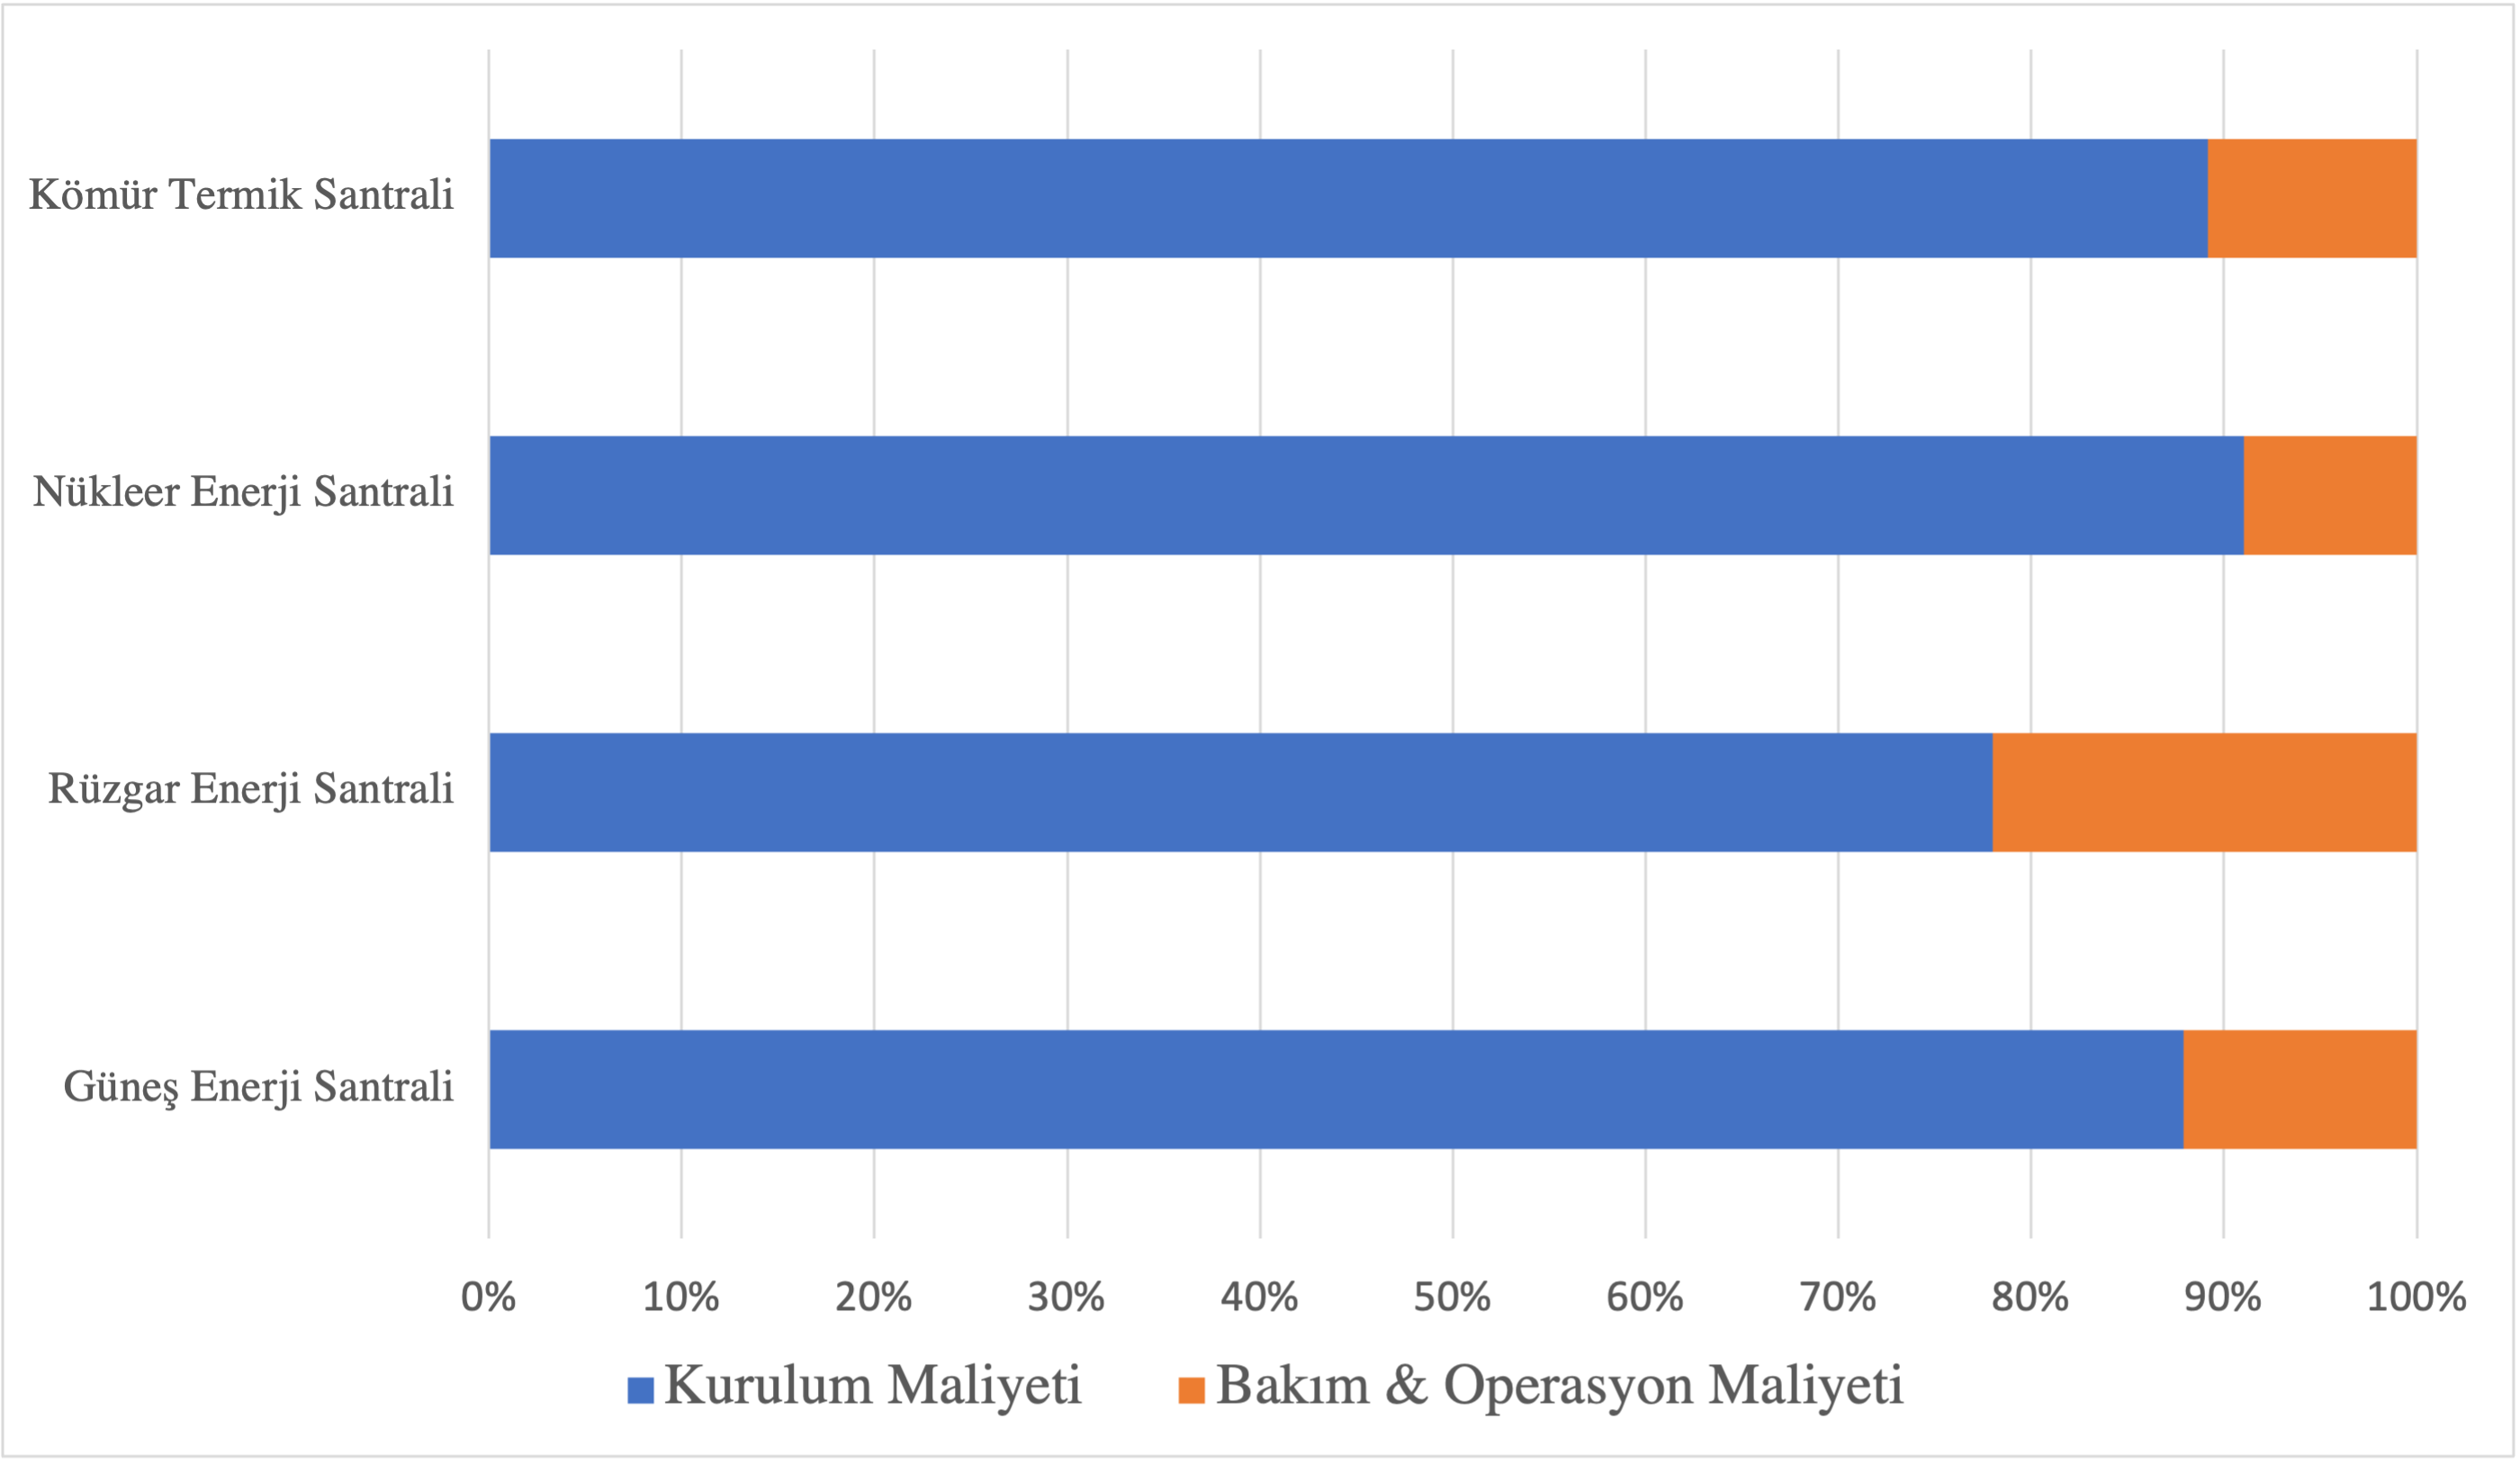
\includegraphics[width=\columnwidth]{Resim/chartbar.png}}
\caption{Enerji santrallerinin maliyet oranları (\protect\citeA{lazardsRapport}) }
\label{fig:Lazards}
\end{figure}

% Preamble: 





Çok etmenli yaklaşım yöntemi kullanılarak yenilenebilir enerji sistemlerinde operasyon ve bakım maliyetlerinin düşürülmesi hakkında yapılan çalışmada ancak ve ancak haberleşme sisteminin etkin bir şekilde kullanılması durumunda ilgili modelin uyaralanabilir olduğu anlaşılmıştır \cite{7804974}. 
Haberleşme sisteminin yenilenebilir enerji kaynaklarında etkin ve verimli bir şekilde kullanılması durumunda enerji üretim maliyetinin alt bileşeni olan bakım onarım ve operasyon giderlerinin maliyetlerine düşüş olacağı kaçınılmazdır.
Enerji üretim maliyetlerine doğrudan etki eden bir diğer unsur ise üretim santrallerinde yaşanan kazalardır. İlgili çalışmada güneş enerji santrallerinde haberleşme sistemine ait düzgün bir altyapının olmadığı durumlarda yaşanan kaza oranlarının daha fazla olduğu gözlemlenmiştir \cite{https://doi.org/10.1002/dac.4517}. Bu kaza durumlarının enerji üretim maliyetlerine doğru orantılı bir şekilde yansıması beklenen bir durumdur.
Mart 2022'de Uydu haberleşme hizmeti veren Euroskypark firmasına düzenlenen siber saldırı sonucu, toplamda yaklaşık 5800 adet rüzgar enerji türbininin haberleşmesi 1 saatliğine kesilmiştir \cite{sibersaldiri}. İlgili türbin topluluğunun üretim potansiyelinin 11 GW değerlerinde olduğu unutulmamalıdır. Haberin detayı incelendiğinde türbinlerin haberleşmesi kapalı durumdayken normal bir şekilde çalışmaya devam ettikleri belirtil-miştir. 11 GW'lık üretim kapasitesindeki bu türbin grubunun faaliyetlerinin 1 saatlik durması veya tamamen çalışmasına aykırı bir şekilde programlandığı durumu düşünül-düğünde yaşanabilecek sorunlar bir hayli maliyet oluşturacaktır.




\section{MOTİVASYON} \label{motivasyon}



Başlık \ref{onem}'de verilen örneklerin sonucu olarak enerji üretim santrallerinin sistemli ve düzgün bir biçimde çalışması için haberleşme altyapısının doğru belirlenmesi şarttır. Bununla birlikte, yaşanacak kazaların ve problemlerin oluşturacağı maliyeti düşür-mek için kullanılan haberleşme sisteminin uygun maliyette ve uygun performans değer-lerinde olması enerji sistemleri yatırımcıları için tercih niteliği taşıyacaktır.

Bu yüksek lisans tezinde, dağıtık enerji üretim santrallerinin gerçek zamanlı olarak takibinin yapılmasına imkan sağlayacak haberleşme çözümlerinin simülasyonları tasarlanmıştır. İlgili simülasyonların performansları ve maliyetleri karşılaştırılarak, ihtiyaca göre en faydalı olacak haberleşme çözümünün belirlenmesi amaçlanmıştır.


\begin{table}[htbp]
\centering
\caption{Literatürde araştırılmış yenilenebilir enerji santrallerinin haberleşme özet tablosu}
\label{tab:literatr}

\begin{tabular}{cp{0.15\textwidth}>{\centering}p{0.12\textwidth}>{\centering}p{0.12\textwidth}>{\arraybackslash}p{0.4\textwidth}}
\hline
\\

No&\multicolumn{1}{c}{Konum}&\multicolumn{2}{c}{Haberleşme Sınıfı}&\multicolumn{1}{c}{Açıklama}\\\cline{3-4}
&&Kablolu&Kablosuz&\\

\\
\hline


1& \cite{BCIT} & Ethernet PLC &Zigbee \gls{wimax} & Üniversite kampüsüne ait 3 adet \gls{res} ve 1 adet \gls{ges} bulunmaktadır.\\
\hline

2& \cite{microgrid_siliOrnek} & Ethernet PLC & GSM & Şili'nin Atacama Çölün'de bulunan Huatacondo köyüne ait 2 adet \gls{ges} , 1 adet \gls{res} ve 1 adet dizel jeneratör sistemi bulunmaktadır.\\
\hline

3& \cite{yunanOrnek} & PLC & \gls{wifi} \gls{gsm} &Termiye Adasınaki köy evlerinin enerji ihtiyacının karşılanması için 2 MW'lık \gls{res}, 100kW'lık \gls{ges} dağıtık yapıda kurulmuştur. \\

\hline


\end{tabular}

\end{table}



Tablo \ref{tab:literatr}'de yenilenebilir enerji santrallerinde kullanılan haberleşme sistemleri hakkında yapılan çalışmaların özeti gösterilmiştir. 1. sırada \gls{bcit} içerisinde faal olarak çalışan yenilenebilir enerji santrallerinin akıllı şebekelere entegrasyonunda kullanılan veri haberleşme altyapısının iyileştirme projesidir \cite{BCIT}. Enstitü içerisinde 3 adet \gls{res}, 1 adet \gls{ges} bulunmaktadır. Enstitü haberleşme ağını 3 kısıma ayırmıştır. \gls{pan} kısmında Zigbee, \gls{lan} kısmında \gls{plc} son olarak \gls{wan} kısmında \gls{wimax} teknolojilerini kullanımıştır. İlgili çalışmada \gls{iec} 61850 standardı dikkate alınarak enerji santrallerinin veri modellenmesi yapılmıştır. Kullanılan veri boyutları maksimum 64 Byte civarı olarak belirlendiğinde, \gls{wimax} \%96 oranında veri iletim performansı göstermiştir. Veri boyutlarının arttırılması sonucunda paket kaybının olmadığı çalışmada gösterilmiştir. Tablo \ref{tab:literatr}'de 2. sırada belirtilen Huatacondo köyünde günlük enerji ihtiyacının \%40'lık kısmını dizel jeneratörlü enerji santralinden karşılamaktadır. Santral bünyesindeki haberleşme altyapısının performans değeri ile dizel jeneratöre olan ihtiyaç yüzdesinin ters orantılı olduğu belirtilmiştir \cite{microgrid_siliOrnek}. Ege Bölgesi'nde bulunan Termiye Adasının enerji ihtiyacı da Huatacondo köyündeki gibi hibrit enerji sistemleri üzerinden karşılanmaktadır. Adada bulunan hane sayısı ve iklim durumları göz önüne alınarak haberleşme sistemlerinin sürdürülebilir yapıda olmasına dikkat edilmiştir. Böylece Termiye Adasında dizel jeneratörlerin kullanım oranlarının düştüğü belirtilmiştir\cite{yunanOrnek}.



Teknolojinin gelişmesiyle birlikte, daha verimli ve daha düşük bakım maliyetlerine sahip rüzgar türbinlerinin üretimi yapılmaktadır. Rüzgar türbinlerinin yönetildiği komuta kontrol merkezleri, elektrik talebine göre açılıp kapatılan rüzgar türbinlerini yönetmek ve kontrol etmekten sorumludur. İlgili makalede rüzgar türbinlerinin güç tüketimini kullanılabilirliğini ve türbin verimliliğini en üst düzeyde kontrolü için tasarlanan iletişim ağ mimarisinden bahsedilmiştir \cite{ahmed2014communication}.

2014 yılında yapılan başka bir çalışmada \cite{hussain2014multilayer} rüzgar enerjisi santralleri gerçek zamanlı izlenmesi ve kontrolü, yüksek güvenilirliğe sahip bir iletişim altyapısı gerektirdiği ile ilgili Ethernet teknolojisini SONET yazılımı aracılığıyla simülasyonu yapılmıştır.

Güneş enerji santrallerini, mevsimsel süreleri, hava durumu ve dağıtık yapıda olması gibi faktörlerden kolayca etkilenebilen bir yenilenebilir enerji sistemidir. Şebeke entegrasyonunun verimini arttırıcı faaliyetler olarak düşük gecikmeli, güvenilir ve iki yönlü iletişim esastır. Şebeke entegrasyonu için \gls{iec} 61850 standardına dayalı büyük ölçekli güneş enerji santrallerinin uzaktan izlenmesi için iletişim ağı mimarisinin tasarlanması ile ilgili çalışmalar yapılmıştır \cite{mackiewicz2006overview}.

Güneşten enerji üretimi ve sistemin kontrolü için \gls{iot} yönteminde Arduino Uno mikrodenetleyicisi ve Rasberry Pi modülleri kullanılarak enerji üretim sisteminin kontrolü ve performansının artırılması yönünde çalışma yapılmıştır. Şekil ~\ref{fig:figure3}'de gösterilmiştir \cite{deshmukh2018smart}.

\begin{figure}[htbp]
%\centerline{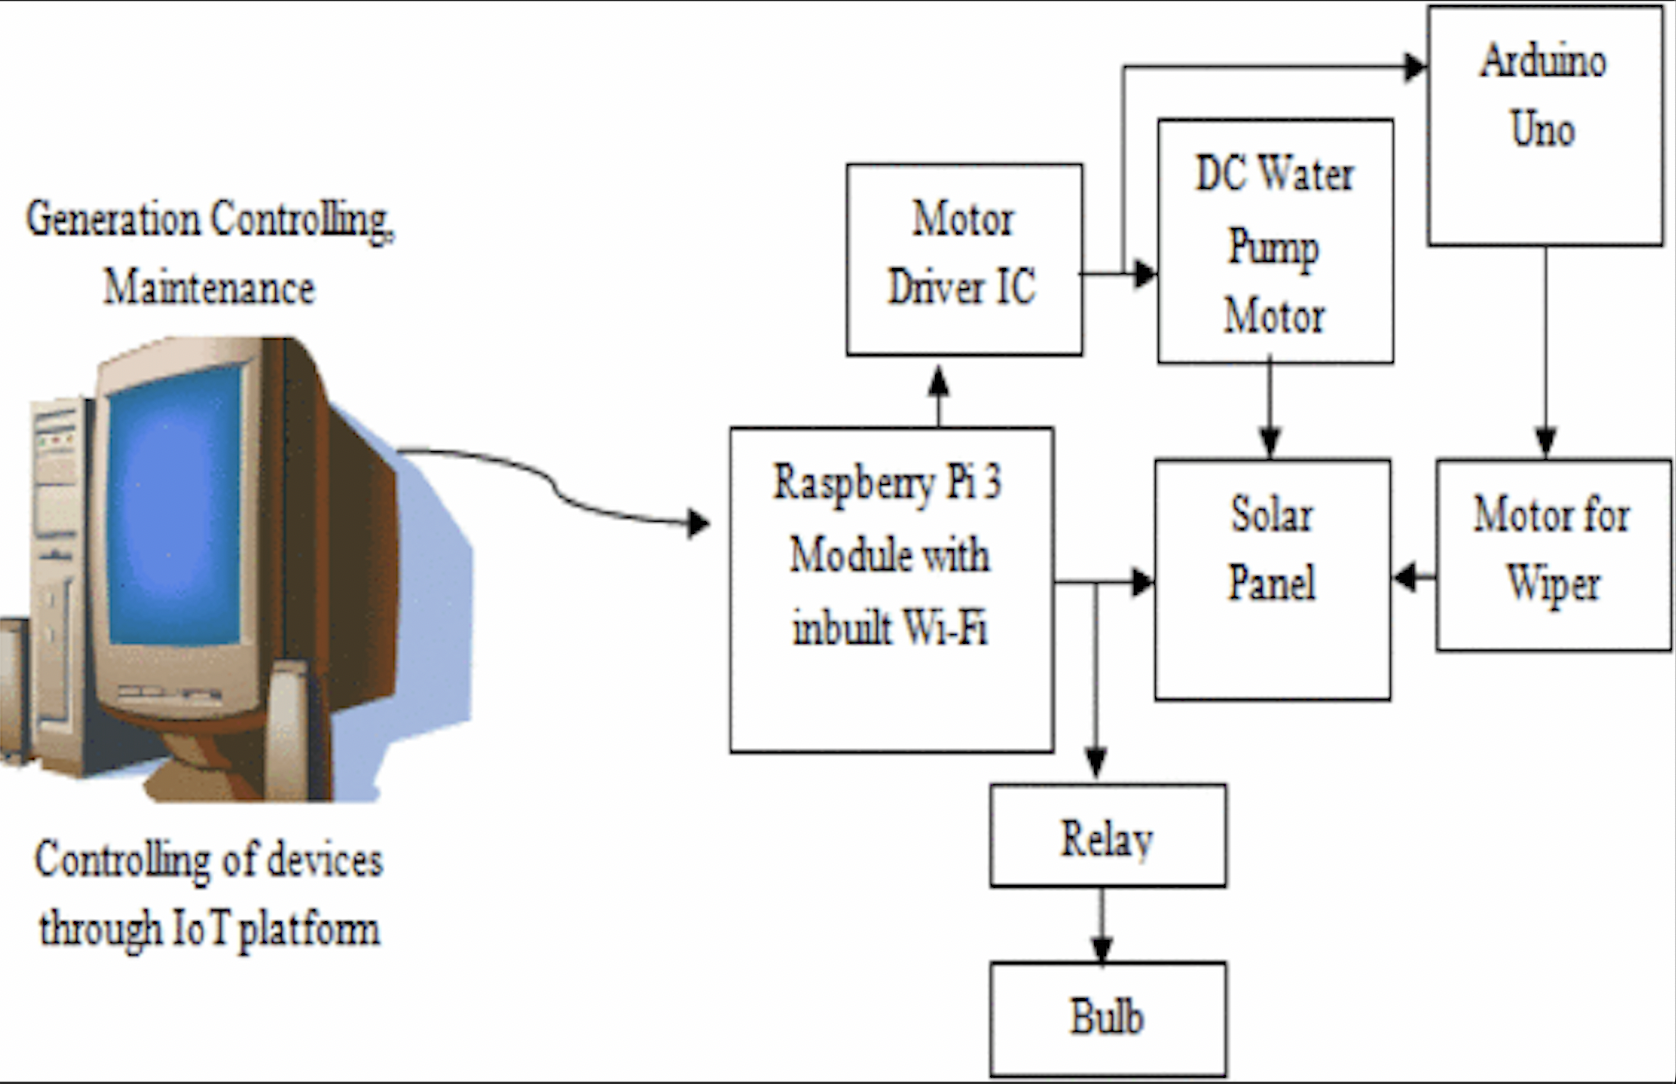
\includegraphics[width=7cm]{Resim/Screenshot 2022-06-12 at 20.44.42.png}}



% Gradient Info
  
\tikzset {_09use7u1u/.code = {\pgfsetadditionalshadetransform{ \pgftransformshift{\pgfpoint{-4 bp } { 0 bp }  }  \pgftransformrotate{0 }  \pgftransformscale{2 }  }}}
\pgfdeclarehorizontalshading{_s630ca86d}{150bp}{rgb(0bp)=(1,1,1);
rgb(37.5bp)=(1,1,1);
rgb(62.5bp)=(0,0,0);
rgb(100bp)=(0,0,0)}
\tikzset{_3228yxobz/.code = {\pgfsetadditionalshadetransform{\pgftransformshift{\pgfpoint{-4 bp } { 0 bp }  }  \pgftransformrotate{0 }  \pgftransformscale{2 } }}}
\pgfdeclarehorizontalshading{_7q59z2lw0} {150bp} {color(0bp)=(transparent!0);
color(37.5bp)=(transparent!0);
color(62.5bp)=(transparent!10);
color(100bp)=(transparent!10) } 
\pgfdeclarefading{_bmhgg1lnn}{\tikz \fill[shading=_7q59z2lw0,_3228yxobz] (0,0) rectangle (50bp,50bp); } 
\tikzset{every picture/.style={line width=0.75pt}} %set default line width to 0.75pt        

\begin{tikzpicture}[x=0.75pt,y=0.75pt,yscale=-1,xscale=1]
%uncomment if require: \path (0,426); %set diagram left start at 0, and has height of 426

%Shape: Rectangle [id:dp7780682150770082] 
\draw  [fill={rgb, 255:red, 155; green, 155; blue, 155 }  ,fill opacity=1 ][line width=0.75]  (159.1,189.62) -- (167.82,189.62) -- (167.82,206.71) -- (159.1,206.71) -- cycle ;
%Shape: Rectangle [id:dp6851387466730021] 
\draw  [fill={rgb, 255:red, 155; green, 155; blue, 155 }  ,fill opacity=1 ][line width=0.75]  (115.1,138.19) -- (212.39,138.19) -- (212.39,193.78) -- (115.1,193.78) -- cycle ;
%Shape: Cube [id:dp0343614423870906] 
\draw   (38.53,153.57) -- (56.53,135.57) -- (98.53,135.57) -- (98.53,225.07) -- (80.53,243.07) -- (38.53,243.07) -- cycle ; \draw   (98.53,135.57) -- (80.53,153.57) -- (38.53,153.57) ; \draw   (80.53,153.57) -- (80.53,243.07) ;
%Shape: Rectangle [id:dp20291484809291327] 
\draw   (44.53,164.78) -- (72.96,164.78) -- (72.96,174.5) -- (44.53,174.5) -- cycle ;
%Shape: Rectangle [id:dp031094078679610115] 
\draw   (47.96,182.35) -- (69.28,182.35) -- (69.28,189.64) -- (47.96,189.64) -- cycle ;
%Shape: Rectangle [id:dp48549901526120576] 
\draw  [fill={rgb, 255:red, 0; green, 0; blue, 0 }  ,fill opacity=1 ] (41.77,229.91) -- (75.63,229.91) -- (75.63,232.48) -- (41.77,232.48) -- cycle ;
%Shape: Rectangle [id:dp25873522519932246] 
\draw  [fill={rgb, 255:red, 0; green, 0; blue, 0 }  ,fill opacity=1 ] (41.77,235.91) -- (75.63,235.91) -- (75.63,238.48) -- (41.77,238.48) -- cycle ;
%Shape: Rectangle [id:dp8233848195769262] 
\path  [shading=_s630ca86d,_09use7u1u,path fading= _bmhgg1lnn ,fading transform={xshift=2}] (121.1,144.07) -- (206.39,144.07) -- (206.39,187.9) -- (121.1,187.9) -- cycle ; % for fading 
 \draw   (121.1,144.07) -- (206.39,144.07) -- (206.39,187.9) -- (121.1,187.9) -- cycle ; % for border 

%Shape: Rectangle [id:dp4973519926476253] 
\draw  [fill={rgb, 255:red, 155; green, 155; blue, 155 }  ,fill opacity=1 ][line width=0.75]  (115.1,206.33) -- (212.39,206.33) -- (212.39,237.21) -- (115.1,237.21) -- cycle ;
%Shape: Trapezoid [id:dp04075975469803139] 
\draw  [fill={rgb, 255:red, 217; green, 214; blue, 213 }  ,fill opacity=1 ] (121.1,209.63) -- (128.39,233.91) -- (199.1,233.91) -- (206.39,209.63) -- cycle ;
%Right Arrow [id:dp5512762508365834] 
\draw   (221.53,165.66) -- (249.84,165.66) -- (249.84,158.87) -- (260.73,167.27) -- (249.84,175.67) -- (249.84,168.87) -- (221.53,168.87) -- cycle ;
%Right Arrow [id:dp6218773129658524] 
\draw   (364.73,165.66) -- (393.04,165.66) -- (393.04,158.87) -- (403.93,167.27) -- (393.04,175.67) -- (393.04,168.87) -- (364.73,168.87) -- cycle ;
%Right Arrow [id:dp25291994634635007] 
\draw   (381.54,168.87) -- (381.54,216.52) -- (388.33,216.52) -- (379.93,234.87) -- (371.53,216.52) -- (378.33,216.52) -- (378.33,168.87) -- cycle ;
%Right Arrow [id:dp7951452337285876] 
\draw   (381.34,270.07) -- (381.34,288.32) -- (388.13,288.32) -- (379.73,300.87) -- (371.33,288.32) -- (378.13,288.32) -- (378.13,270.07) -- cycle ;
%Right Arrow [id:dp2588197140672288] 
\draw   (336.2,140.25) -- (336.2,116.72) -- (329.4,116.72) -- (337.8,107.67) -- (346.2,116.72) -- (339.4,116.72) -- (339.4,140.25) -- cycle ;
%Bend Arrow [id:dp384581087261866] 
\draw   (402.5,77.25) -- (402.5,26.51) .. controls (402.5,26.51) and (402.5,26.51) .. (402.5,26.51) -- (501.5,26.51) -- (501.5,20) -- (519,29.38) -- (501.5,38.75) -- (501.5,32.24) -- (408.23,32.24) .. controls (408.23,32.24) and (408.23,32.24) .. (408.23,32.24) -- (408.23,77.25) -- cycle ;
%Right Arrow [id:dp3009728022088294] 
\draw   (387.73,77.66) -- (417.89,77.66) -- (417.89,70.87) -- (429.5,79.27) -- (417.89,87.67) -- (417.89,80.87) -- (387.73,80.87) -- cycle ;
%Right Arrow [id:dp4821741578803411] 
\draw   (546.04,61.87) -- (546.04,109.52) -- (552.83,109.52) -- (544.43,127.87) -- (536.03,109.52) -- (542.83,109.52) -- (542.83,61.87) -- cycle ;
%Right Arrow [id:dp9449968586875006] 
\draw   (518.5,162.87) -- (474.98,162.87) -- (474.98,169.67) -- (458.23,161.27) -- (474.98,152.87) -- (474.98,159.66) -- (518.5,159.66) -- cycle ;

% Text Node
\draw (137.93,96.67) node   [align=left] {\begin{minipage}[lt]{98.6pt}\setlength\topsep{0pt}
\begin{center}
{\footnotesize {\fontfamily{ptm}\selectfont IoT Üzerinden}}\\{\footnotesize {\fontfamily{ptm}\selectfont Kontrol \& Bakım}}
\end{center}

\end{minipage}};
% Text Node
\draw    (260.53,139.47) -- (364.53,139.47) -- (364.53,193.47) -- (260.53,193.47) -- cycle  ;
\draw (312.53,166.47) node   [align=left] {\begin{minipage}[lt]{68pt}\setlength\topsep{0pt}
\begin{center}
{\footnotesize {\fontfamily{ptm}\selectfont Rapsberry Pi 3}}
\end{center}

\end{minipage}};
% Text Node
\draw    (404.43,139.87) -- (457.43,139.87) -- (457.43,193.87) -- (404.43,193.87) -- cycle  ;
\draw (430.93,166.87) node   [align=left] {\begin{minipage}[lt]{33.59pt}\setlength\topsep{0pt}
\begin{center}
{\footnotesize {\fontfamily{ptm}\selectfont Güneş}}\\{\footnotesize {\fontfamily{ptm}\selectfont Paneli}}
\end{center}

\end{minipage}};
% Text Node
\draw    (361.43,236.07) -- (398.43,236.07) -- (398.43,270.07) -- (361.43,270.07) -- cycle  ;
\draw (379.93,253.07) node   [align=left] {\begin{minipage}[lt]{22.3pt}\setlength\topsep{0pt}
\begin{center}
{\footnotesize {\fontfamily{ptm}\selectfont Röle}}
\end{center}

\end{minipage}};
% Text Node
\draw    (352.23,301.07) -- (407.23,301.07) -- (407.23,335.07) -- (352.23,335.07) -- cycle  ;
\draw (379.73,318.07) node   [align=left] {\begin{minipage}[lt]{34.82pt}\setlength\topsep{0pt}
\begin{center}
{\footnotesize {\fontfamily{ptm}\selectfont İndikatör}}
\end{center}

\end{minipage}};
% Text Node
\draw    (272.77,53.87) -- (386.77,53.87) -- (386.77,107.87) -- (272.77,107.87) -- cycle  ;
\draw (329.77,80.87) node   [align=left] {\begin{minipage}[lt]{74.66pt}\setlength\topsep{0pt}
\begin{center}
{\footnotesize {\fontfamily{ptm}\selectfont Motor}}\\{\footnotesize {\fontfamily{ptm}\selectfont Sürücü}}
\end{center}

\end{minipage}};
% Text Node
\draw    (428.87,54.37) -- (511.87,54.37) -- (511.87,108.37) -- (428.87,108.37) -- cycle  ;
\draw (470.37,81.37) node   [align=left] {\begin{minipage}[lt]{53.9pt}\setlength\topsep{0pt}
\begin{center}
{\footnotesize {\fontfamily{ptm}\selectfont Su}}\\{\footnotesize {\fontfamily{ptm}\selectfont Motoru (DC)}}
\end{center}

\end{minipage}};
% Text Node
\draw    (519.93,7.87) -- (572.93,7.87) -- (572.93,61.87) -- (519.93,61.87) -- cycle  ;
\draw (546.43,34.87) node   [align=left] {\begin{minipage}[lt]{33.59pt}\setlength\topsep{0pt}
\begin{center}
{\footnotesize {\fontfamily{ptm}\selectfont Arduino}}\\{\footnotesize {\fontfamily{ptm}\selectfont Uno}}
\end{center}

\end{minipage}};
% Text Node
\draw    (518.43,127.87) -- (571.43,127.87) -- (571.43,181.87) -- (518.43,181.87) -- cycle  ;
\draw (544.93,154.87) node   [align=left] {\begin{minipage}[lt]{33.59pt}\setlength\topsep{0pt}
\begin{center}
{\footnotesize {\fontfamily{ptm}\selectfont Silecek}}\\{\footnotesize {\fontfamily{ptm}\selectfont Motoru}}
\end{center}

\end{minipage}};


\end{tikzpicture}



\caption{Bir \gls{res}'in \gls{iot} üzerinden izlenmesi ve kontrolü}
\label{fig:figure3}
\end{figure}


Dağıtım şebekelerinde \gls{wimax} ve \gls{wifi} teknolojilerinin, şebeke maliyetinde ve performansındaki durumlarını olumlu yönde etkilediği ile ilgili bir makale çalışılması yapılmış olup, Şekil ~\ref{fig:figure4}'de kurulan topoloji gösterilmiştir \cite{wlanwimaxprem}.


\cite{eltamaly2021iot} enerji sistemlerinde haberleşme alanında yaptığı çalışmalarda, akıllı şebekelerde kullanılan haberleşme sistemlerini inceleyip 4 katmanda toplamıştır. İlgili katmanların paket gecikme performanslarını incelemiştir.

\begin{figure}[htbp]
\centerline{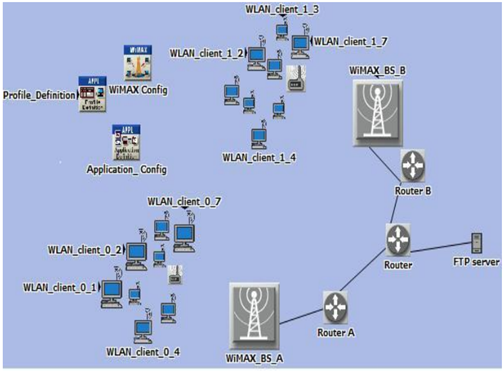
\includegraphics[width=12cm]{Resim/Sekil2-3.png}}
\caption{\gls{res} haberleşme topolojisi (\protect\citeA{wlanwimaxprem}) }
\label{fig:figure4}
\end{figure}

Akıllı şebekelerin haberleşme altyapılarındaki performans değerleri simülasyon ortamında kurulup incelenmiştir. İlgili çalışmada fiber optik, \gls{wifi} ve \gls{lora} teknolojileri tek bir senaryoda sırasıyla konfigüre edilmiştir ve performans analizleri paylaşılmıştır \cite{yuan2020modeling}. 



Teknolojinin gelişmesi ile birlikte enerji üretim santrallerinin de donanımsal açıdan yeni tasarımları yapılmaktadır. Rüzgar türbinlerinin fiziksel özellikleri de bu değişimden olumlu yönde etkilenmektedir. Günümüzde rüzgar türbinleri okyanuslarda, dağlık arazilerde daha verimli bir şekilde enerji üretmektedirler. \cite{liu2010status} \gls{res}'lerde \gls{wimax} tekniği kullanılması durumunda oluşacak performans değerlerini gözlemlemiştir.




Türbin sayısının artmasından kaynaklı yerleşke olarak uzak noktaların tercih edildiği rüzgar tarlalarının çalışma, üretim ve arıza durumlarının minimum gecikmeyle izlenmesi için hiyerarşik ağ yapısı yöntemiyle birden fazla komuta kontrol merkezinin haberleşme trafiğinin yönetimi ile ilgili çalışma yapılmıştır \cite{hussain2014multilayer}. Oluş-turulan mimarinin gösterimi Şekil ~\ref{fig:figure6}'de paylaşılmıştır .






\begin{figure}[htbp]
\centerline{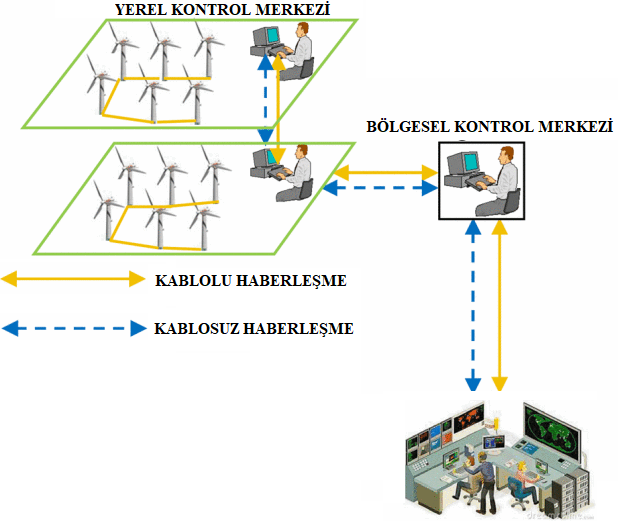
\includegraphics[width= 8 cm]{Resim/Screenshot 2022-06-12 at 21.27.08.png}}
\caption{Yenilenebilir enerji sistemlerinde hiyerarşik durum kontrol sistemi (\protect\citeA{hussain2014multilayer}) }
\label{fig:figure6}
\end{figure}

\part{GELİŞTİRİLEN YÖNTEM}
\thispagestyle{empty}
\newpage
\section{YENİLENEBİLİR ENERJİ SİSTEMLERİ İÇİN\\DAĞITIK ALGILAYICI AĞ MİMARİLERİ: DPÜ MODELİ}

 Başlık \ref{motivasyon} bize haberleşme sistemlerinin enerji sistemlerinde nasıl kullanıldığı hakkında geçmişte yapılmış olan araştırmaları özetlemiştir. \gls{dpu}'de tüm enerji ihtiyacını yenilenebilir kaynaklardan karşılaması için bir çalışma yapılması durumu düşünüldüğünde, bu tezin \ref{motivasyon} ve \ref{onem} kısımlarında bahsi geçen konular dikkate alınması gerekmektedir. Çünkü enerji sisteminde karşılaşılan problemlerin sonuçları, ilgili sistemlerin sahibine maddi açıdan yüklü maliyetler oluşturabilir. İlgili sorunların önüne geçilmesi için \gls{dpu}’ye ait tüm eğitim lokasyonlarının aktif ve sürekli bir şekilde merkezi bir yapıdan enerji üretiminin izlenmesi, kontrolünün sağlanması ve olası problemleri önceden tahmin edebilmesi için üretim sistemlerine ait tüm cihazların durum ve faaliyetleri hakkındaki veri trafiğini incelemesi gerekir. \gls{dpu}’ye ait lokasyonlarda güneş veya rüzgar enerji santrallerinin kurulduğu varsayılmıştır. Tezin giriş kısmında belirtilen rüzgar ve güneş enerji sistemlerinin dışındaki diğer yenilenebilir enerji sistemleri bu yüksek lisans tezinde incelenmemiştir.

Güneş enerjisi ve rüzgar enerji santrallerinin kapasite faktörünün düşük olma-sının temel nedeni genellikle enerji kaynağının her zaman kullanılabilir olmaması durumundan kaynaklıdır. Tesis elektrik üretebiliyor olabilir, ancak "yakıtı" (rüzgar, güneş ışığı) mevcut olmayabilir. Bununla birlikte, güneş, rüzgar santralleri yüksek kullanılabi-lirlik faktörlerine sahiptir, bu nedenle mevcut yakıtları olduğunda neredeyse her zaman elektrik üretebilirler. Genelleme yapıldığında Rüzgar tarlalarında kapasite faktörü \%20--40 arasında olurken, güneş panellerinde \%15--30 arasında olmaktadır \cite{hussain2014multilayer}. Türkiye Cumhuriyeti Enerji ve Tabii Kaynaklar Bakanlığı’nın yayınlamış olduğu enerji haritalarından Kütahya’ya ait rüzgar ve güneş enerji kapasitelerini Şekil \ref{fig:figure7}--\ref{fig:figure8} üzerinde gösterilmiştir \cite{gepa}\cite{repa}. İlgili resimlerle gösterilmiş olan kapasite faktörleri değerlendirilmiştir. Buna göre üniversite yerleşkelerine kurulması muhtemel enerji sistemleri Tablo \ref{tab:tabb1}'de gösterilmiştir.

\begin{figure}[htbp]
\centerline{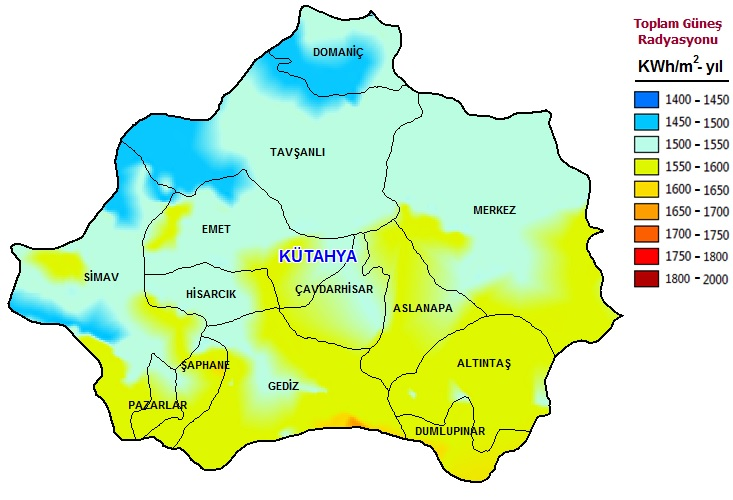
\includegraphics[width=\columnwidth]{Resim/Sekil3-1.jpg}}
\caption{Kütahya bölgesi güneş enerjisi atlası  (\protect\citeA{gepa}) }
\label{fig:figure7}
\end{figure}

%\section{Enerji Üretilecek Yöntemin Seçimi}


\section{HABERLEŞME AĞI TASARIM KONSEPTİ}

İletişim, bir organizasyonun başarısındaki en önemli faktörlerden biridir. Bir kurum, ancak haberleşme ağ altyapısı güçlüyse, iş akış ve takip süreçleri kolaylaşır sürdürü-lebilir bir yapıda olur. Bu nedenle organizasyonlar ve kurumlar arasında kapsamlı bir şekilde haberleşme yapıları kurulmuştur. Ağ hizmetleri, ağın uygulanmasını, yönetimini, bakımını ve izlenmesini gibi görevleri üstlene bir yapıdır. Buna göre ağ hizmetlerinin sorunsuz bir şekilde sağlanması için hizmette kullanılan bileşenler aşağıdaki başlıklarda incelenmiştir.



\begin{figure}[htbp]
\centerline{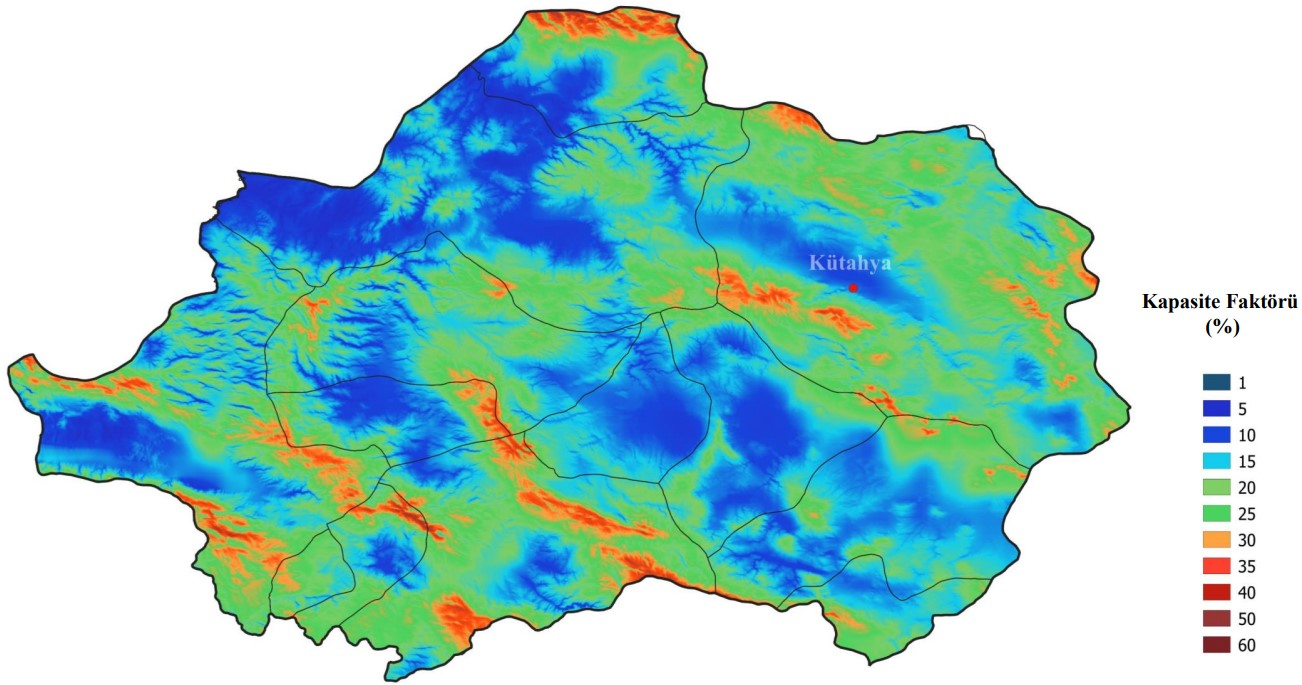
\includegraphics[width=\columnwidth]{Resim/Sekil3-2.jpg}}
\caption{Kütahya bölgesi rüzgar enerjisi atlası  (\protect\citeA{repa}) }
\label{fig:figure8}
\end{figure}

\begin{table}[htbp]
\centering
\caption{\gls{dpu}'nün yerleşkelerinde kurulacak olan enerji sistemlerinin tablosu}
\label{tab:tabb1}
\begin{tabular}{clccc}
\hline
No & \multicolumn{1}{c}{Yerleşke İsmi} & \multicolumn{1}{c}{Enerji Sistemi} & Enlem & Boylam \\ \hline
1  & ALTINTAŞ \gls{myo}    & \gls{ges}  & 39.07502 & 30.13237 \\
\hline
2  & ÇAVDARHİSAR \gls{myo} & \gls{ges}  & 39.18129 & 29.60534 \\
\hline
3  & DOMANİÇ \gls{myo}     & \gls{res} & 39.80160 & 29.60133 \\
\hline
4  & EMET \gls{myo}        & \gls{res} & 39.33699 & 29.26823 \\
\hline
5  & GEDİZ \gls{myo}       & \gls{ges}  & 39.00807 & 29.40444 \\
\hline
6  & GERMİYAN \gls{myo}    & \gls{res} & 39.39076 & 30.03973 \\
\hline
7  & HİSARCIK \gls{myo}    & \gls{res} & 39.25412 & 29.22920 \\
\hline
8  & PAZARLAR \gls{myo}    & \gls{ges}  & 28.99846 & 29.12381 \\
\hline
9  & ŞAPHANE \gls{myo}     & \gls{ges}  & 39.02577 & 29.22203 \\
\hline
10 & SİMAV \gls{myo}       & \gls{res} & 39.11189 & 29.01717 \\
\hline
11 & TAVŞANLI \gls{myo}    & \gls{res} & 39.56802 & 29.45904\\
\hline

\end{tabular}
\end{table}
\subsection{Ağ Bileşenleri}

Tezin giriş kısmında bahsedildiği üzere iletişim olanakları arasında telefon hatları, koaksiyel kablolar, mikrodalga bağlantıları, uydu kanalları ve optik fiberler bulunmaktadır. Bu fiziksel ortamların her biri, iletişimi sağlama yeteneği açısından farklı özelliklere sahiptir. Ağ tasarımının kriterleri genelde maliyet, kapasite ve güvenilirlik olarak 3 kısımdan oluştuğunu düşünebiliriz. Aylık kiralama maliyeti, kurulum maliyeti, birim trafik başına maliyet ve bakım onarım maliyeti olarak olarak dört kısımda toplanır. Ağ tasarımındaki metodolojiye göre bu maliyetler hesaplanır. Kapasite tarifi genelde veri haberleşmesi olduğundan bit/s olarak saniyede taşınan veri miktarı olarak tanımlanır. Haberleşme uygulamalarında toplam kapasitenin tamamında haberleşme mesajları bulunmamaktadır. Sayısal haberleşmede kullanılan bir takım haberleşme protokolleri verinin önüne ve sonuna protokol mimarisini anlatan veri paketleri üretmektedir. Bu yüzden kullanılabilir kapasite ile toplam kapasite arasında veri boyutu farkı oluşmaktadır. Güven Oranı hesabı bir kanalın faal ve gayri faal olduğu zamanın oranı olarak tanımlanabilir. Bu tanıma göre gayri faal olma aralığı (GFOA) ile gayri faal süresi (GFS) bileşenleriyle Denklem \eqref{eq1}'de hesaplanır. 

\begin{equation}
\text{Güven Oranı} = 1 - (\text{ GFS / GFOA } ) \label{eq1}
\end{equation}


Haberleşme ağlarının oluşumunda kullanılan cihazlara genelde düğüm olarak isim verilmektedir. Ağ düğümlerini aşağıdaki gibi sınıflara ayırabiliriz \cite{parziale_2006}.




\subsubsection{Hub(Cihaz Aktarıcı)}

Hub'lar, birden çok ağ aygıtını birbirine bağlar. Hub aynı zamanda bağlantı kabloları üzerinden uzun mesafeler kat ettikten sonra bozulan sinyalleri güçlendirdiği için bir tekrarlayıcı görevi görür. Hub, yerel ağ bileşenlerini aynı protokollerle bağladığı için ağ bağlantı cihazları ailesinde en basit olanıdır.

Verilerin biçimlendirilmesine hazırlanmak üzere yapılandırılması koşuluyla hem sayısal hem de analog verilerle kullanılabilir. Örneğin, gelen veri sayısal formatta ise, hub bunu paketler halinde iletmesi gerekir; ancak gelen veri analog ise, hub bunu sinyal biçiminde iletir.

Hub'lar, paket filtreleme veya adresleme işlevleri gerçekleştirmez; sadece bağlı tüm cihazlara veri paketleri gönderirler \cite{parziale_2006}.




\subsubsection{Switch (Ağ Anahtarı)}

Genellikle Hub’dan daha akıllı cihazlar olarak sınıflandırılır. Anahtar, ağdaki düğümler hakkında sınırlı yönlendirme bilgilerini korur ve hub’lar veya yönlendiriciler gibi sistemlere bağlantı izni verir. Yerel ağ tasarımında genelde anahtar kullanılır.

Anahtarların sahip olduğu sanal ağ yapılandırma tekniği sayesinde hublara göre çok tercih edilir. Anahtarların ağ güvenliği sanal ağ yapılandırma tekniğinden dolayı daha güvenlidir \cite{parziale_2006}.



\subsubsection{Yönlendirici (Router)}

Farklı ağ topolojilerinin kullanılmış olduğu yapılar arasında çizilen patikadaki veri trafiğini sağlayan cihazlara yönlendirici tanımı yapılmaktadır. Yönlendiriciler akıllı cihazlardır ve bağlı oldukları ağlar hakkında bilgi depolarlar. Yönlendiriciler, geniş alan ağlarında kapsayacak şekilde bir tasarıma geçmektedir. birden çok yerel ağı birbiriyle haberleştirmeyi sağlar. Haberleştirme sırasında tanımlanan veri trafiklerine göre rotalar oluşturur. Bu tür yönlendiricilere sınır yönlendirici ismi de verilmektedir  \cite{parziale_2006}.

\subsubsection{Köprü (Bridge)}


Köprüler, yalnızca fiziksel veri bağlantı katmanlarında çalışmaktadır. Köprüler, iki fiziksel ağın arasında kurulur ve ikisi arasındaki veri akışını yönetir. Hub donanımına benzer bir yapısı vardır. Fakat veri paketlerini iletmeden önce hedef adresler için filtreleme özelliğini yapar. Köprüler işlevsellik açısından anahtarlardan daha az özelliğe sahiptirler. Maliyet açısından anahtarları kullanmak daha çok tercih edilmektedir \cite{parziale_2006}.


\subsubsection{Algılayıcı Düğümleri (Sensor Node)}\label{algilayicidugum}

Algılayıcı düğümleri, bu tezde kullanılan temel donanımdır. Çünkü enerji sistemlerinde üretilen bütün veriler bu algılayıcı düğümlerinde oluşturulacaktır. Çevresel durumları ölçerek haberleşme altyapısına uyacak veri şekillendirmesini yapar ve veri aktarım standartlarına göre veriyi hazırlayıp çalıştığı yerel ağına bağlı olan sunucuya ölçmüş olduğu algılayıcı verilerini gönderirler. Algılayıcıların göndermiş olduğu veri detayları 4. bölümde verilecektir \cite{parziale_2006}.

\begin{figure}[htbp]
\centerline{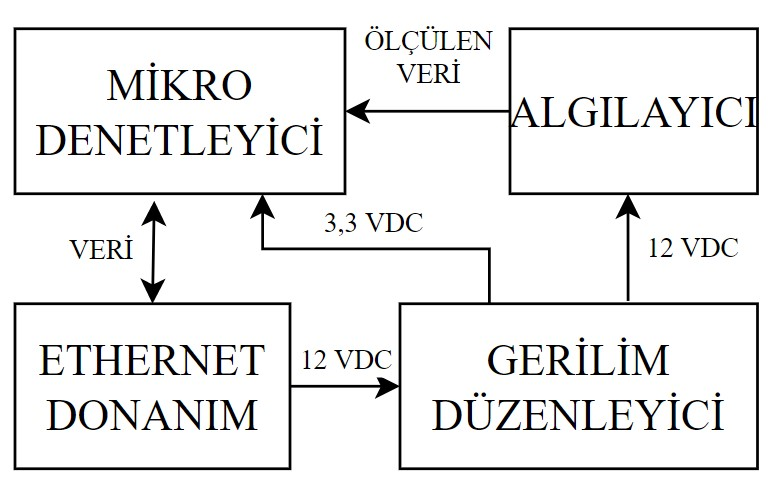
\includegraphics[width=7cm]{Resim/sekil3-3.jpg}}
\caption{Ethernet tipi algılayıcı düğümü gösterimi}
\label{fig:figure9}
\end{figure}

Şekil ~\ref{fig:figure9}'teki resme bakıldığında ethernet tabanlı algılayıcı düğümünün blok diyagramı gösterilmiştir. Haberleşme trafiği ve cihazın ihtiyaç DC gerilim ethernet kablosuyla aktarılmaktadır.


\begin{figure}[htbp]
\centerline{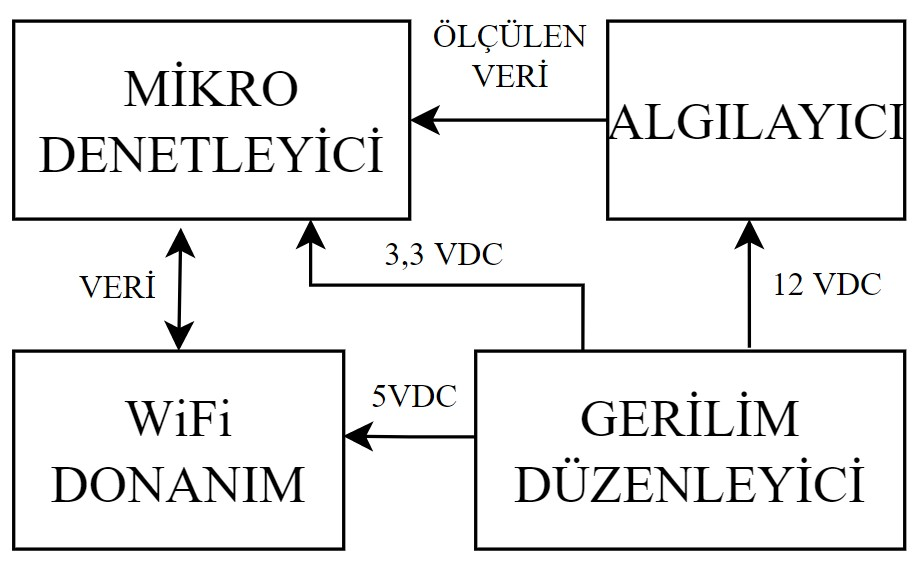
\includegraphics[width=7cm]{Resim/sekil3-4.jpg}}
\caption{Kablosuz tipi algılayıcı düğümü gösterimi}
\label{fig:figure10}
\end{figure}

Şekil ~\ref{fig:figure10}'teki resme aynı algılayıcı düğümünün kablosuz haberleşme modelinin blok diyagramı paylaşılmıştır.

\subsection{Haberleşme Ağ Sınıfları}


\subsubsection{Kişisel Alan Ağı (PAN)}
Cihazlar arası çok düşük mesafede haberleşme imkanı sağlayan ağlara kişisel alan ağı denir \cite{tanenbaum2002computer}.

\begin{figure}[htbp]
\centerline{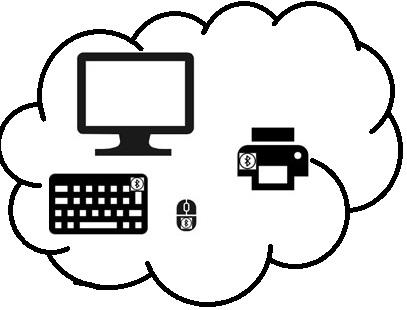
\includegraphics[width=8cm]{Resim/Sekil3-5.jpg}}
\caption{Bilgisayara bağlı olan bluetooth bağlantılı cihazların oluşturduğu \gls{pan} ağı gösterilmiştir.}
\label{fig:figure11}
\end{figure}

\subsubsection{\gls{lan}}
\gls{lan}'lar, kişisel bilgisayarın veya elektronik cihazların bilgi alışverişinde bulunmalarına izin vermek için oluşturulan ağa denir. Günümüzde özellikle kablosuz yerel ağlar kolayca gözlemlenebilir. Kafeteryadaki kablosuz ağlara kişisel bilgisayarları, telefonları veya tablet bilgisayarlarıyla bağlanan kişiler, aslında internet hizmetinden faydalanabilmek için yerel ağa bağlanmış olurlar. Kablosuz ağa dahil olabilmek için gereken anten modülüne sahip ağ adaptörünün olmasıdır. Genelde bilgisayarlar ve elektronik cihazlar kablosuz bir şekilde haberleşme yapabilmek için Erişim Noktası (Access Point), kablosuz yönlendirici veya baz istasyonlarına bağlanırlar \cite{tanenbaum2002computer}.

\begin{figure}[htbp]
\centerline{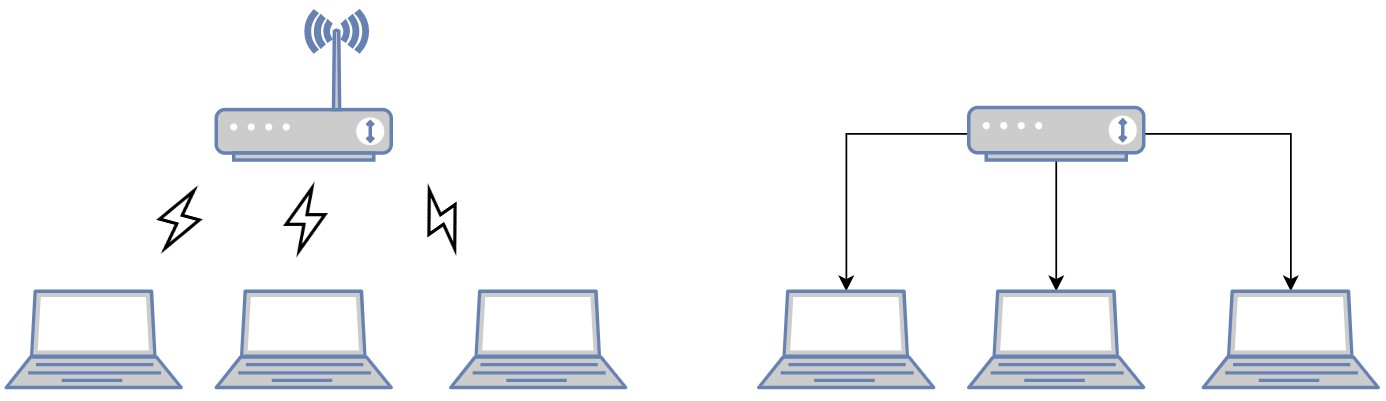
\includegraphics[width=\columnwidth]{Resim/Sekil3-6.jpg}}
\caption{\gls{lan} gösterimi.}
\label{fig:figure12}
\end{figure}

\subsubsection{MEtropolitan Alan Ağı (\gls{man})}

\gls{man}'ın en bilinen örnekleri kablolu televizyonlardır. İletişim firmaları tüm şehirleri kablolamak için yerel yönetimlerle sözleşme üzerinden televizyon yayını için altyapı çalışmalarında bulunmuştur. Televizyonun yayın trafiği için tasarlanan kabloları, internetin geniş bir kitleyi kendine çekmeye başladığı zaman, kablolu TV şebekesi operatörleri, sistemde yapılacak bazı değişikliklerle, yayın spektrumunun kullanılmayan kısımlarında iki yönlü internet hizmeti sağlayabileceklerini buldular. Bu noktada, kablolu TV sistemi, televizyonu bir \gls{man} dağıtmanın basit bir yolundan dönüşmeye başladı. İlk yaklaşıma göre, bir \gls{man} Şekil \ref{fig:figure13}'de gösterilen topoloji gibidir. Bu şekilde, hem televizyon sinyalleri hem de internet daha sonra insanların evlerine dağıtılmak üzere merkezi kablolu modem sonlandırma sistemine evrilmiştir. \cite{tanenbaum2002computer}.


\begin{figure}[htbp]
\centerline{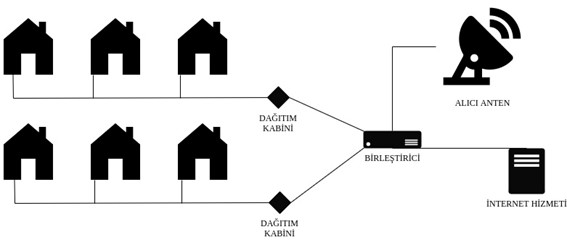
\includegraphics[width=10cm]{Resim/Sekil3-7.jpg}}
\caption{\gls{man} örnek gösterimi.}
\label{fig:figure13}
\end{figure}

\subsubsection{\gls{wan}}

\gls{wan}, geniş bir coğrafi alanı, genellikle bir ülkeyi, bir kıtayı ve hatta birden çok kıtayı kapsar. Geniş bir ağ, bir kurumsal geniş alan ağı durumunda olduğu gibi özel bir kuruluşa hizmet edebilir veya bir transit ağ durumunda olduğu gibi ticari bir hizmet sunumu olabilir.
İzmir, Ankara, Sinop şehirlerinde şubeleri olan bir şirket örneğine ait bir \gls{wan} sistemi aşağıdaki şekilde gösterilmiştir. Bu şubelerin her biri, kullanıcı programlarını çalıştırmaya yönelik bilgisayarlar içerir. Şekilde gösterilen her şubeye ait makineler ana bilgisayar (host) olarak adlandırılır. Bu ana bilgisayarları birbirine bağlayan ağın geri kalanına iletişim alt ağı(subnet) denir. Telefon sisteminin sözcükleri konuşmacıdan dinleyiciye taşıması gibi, alt ağ da mesajları ana bilgisayardan ana bilgisayara taşır.
Çoğu geniş alan ağında, alt ağ iki farklı bileşenden oluşur: iletim hatları ve anahtarlama elemanları. İletim hatları sayesinde veriler makineler arasında taşınır. Bakır tel, koaksiyel kablo, optik fiber veya radyo teknolojileri iletim hatlarına örnek olarak gösterilir. Aşağıdaki resimde geniş alan ağı gösterilmiştir \cite{tanenbaum2002computer}.

\begin{figure}[htbp]
\centerline{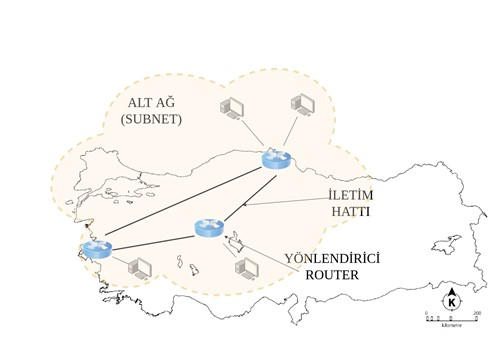
\includegraphics[width=8cm]{Resim/Sekil3-8.jpg}}
\caption{\gls{wan} örnek gösterimi.}
\label{fig:figure14}
\end{figure}


\subsection{Ağ Tasarım Yazılımı}

Ağ tasarım programlarının dünyada önemli bir rolü vardır. Çünkü haberleşme ağlarının sahada kurulumundan önce maliyet analizi ve performansının hesaplanması için çok bileşen bulunmaktadır. Piyasadaki ağ tasarım programları sayesinde, saha uygulaması yapılmadan maliyet hesabını ve uygulanabilirliğinin analizi mümkündür. \gls{opnet} yazılımı piyasada kullanılan en popüler ağ tasarım yazılımlarından birisidir. \gls{opnet} açık kaynaklı bir ürün değildir. Erişim ve kullanım için lisansa ihtiyaç bulunmaktadır. Özellikle ticari amaçlarla kullanılmasından kaynaklı olarak, kendi sitesinde ve haberleşme ağları tasarım dünyasında \gls{opnet} hakkında yazılmış çok sayıda kitap ve makale bulunmaktadır. \gls{opnet} yazılımın özellikleri;

•	Kolay bir grafik arayüzüne sahiptir.

•	Kullanıcılara zengin bir ağ modeli ve ağ tasarım kütüphanesi sunmaktadır.

•	Kullanıcı kolayca senaryo analizini yapabilmektedir.

•	Kurulumu diğer ağ tasarım programlarına göre daha kolaydır.

•	Grafik arayüzleri ile gerçek zamanlı bir simülasyon ortamı sağlar.

•	Ticari bir program olmasından kaynaklı güvenilir ve verimlidir.


\gls{opnet} çalışma prensibi olarak 4 bölümden oluşmaktadır. 

•	Model tasarımı

•	İstatistiklerin seçimi

•	Simülasyonun çalıştırılması

•	Elde edilen sonuçların görüntülenmesi ve analizi


Haberleşme ağlarında optimizasyon konulu bu yüksek lisans tezinde \gls{opnet} Akademik lisanslı yazılım kullanılarak simülasyon yapılmıştır. \cite{FITPUB8317}
\part{SİMÜLASYON MODELİ}
\thispagestyle{empty}
\newpage
\section{YENİLENEBİLİR ENERJİ SİSTEMLERİNDE KULLANILAN ALGILAYICILARIN VERİ YAPILARI}

Yenilenebilir enerji sistemlerinde veri transfer standartlarını oluşturabilmek için \gls{iec} 61850 iletişim standardı kullanılır. İlgili standart kullanılarak enerji santrallerinde oluşturulan veriler kontrol, gözlem ve enerji sistemlerinde oluşabilecek arızaların gerçek zamanlı şekilde kontrolünün sağlanması amaçlanmıştır \cite{1385190}. Rüzgar enerji türbinleri ve güneş enerji panellerinde oluşturulacak sistemsel çalışma verilerinin aktif bir şekilde kontrolü amaçlanmıştır. Bu kontrolün sağlanması için \gls{iec} 61850 ve benzer standartlardan olan \gls{iec} 61400-25 standartları dikkate alınmıştır \cite{Olsen_prototypeof} \cite{francisco2016protection}.


\subsection{Rüzgar Enerji Sistemlerinde Veri Yapıları}
Eskiden, rüzgar enerji türbinleri ile kontrol odası arasındaki iletişim sistemi, enerji üretimi işini yüklenen firmalar tarafından belirli bir standarda bağlı olmadan çözül-mekteydi. Bu durum yüklenici firmaların hepsinde kendisine özel bir çözüm oluşturmaya sebebiyet vermiştir. Danimarkalı büyük bir türbin firması ilgili haberleşme çözümü için \gls{iec}'ye başvuruda bulunmuştur. Bu başvuru sayesinde \gls{res}'lerin haberleşme standarlarından \gls{iec} 61400 standardı geliştirilmiştir \cite{Olsen_prototypeof}.

\gls{iec} 61400-25 standardı, rüzgar enerjisi santrallerinin izlenmesi ve kontrolü için birleşik bir iletişim sisteminin tanımlanması ve standartlaştırılması için özel bir versiyondur. \gls{iec} 61400-25 serisi, genel olarak trafo merkezlerindeki iletişim ağlarını ve sistemleri tanımla-yan \gls{iec} 61850 serisi standartların bir uzantısıdır. 


\gls{iec} 61400-25 standardı sayesinde, enerji üretim sistemindeki algılayıcılardan oluşan veriler sayısal haberleşme standartlarında tekrardan yapılandırılıp komuta kontrol merkezlerine iletilir. IEC 61400 5 kategoriye ayrılır.

•	Genel tanımlar ilkeler ve modeller (\gls{iec} 61400-25-1).

•	Rüzgar türbinlerinin enformasyon model standardı (\gls{iec} 61400-25-2).

•	Enformasyon değişim model standardı (\gls{iec} 61400-25-3).

•	İletişim profilinde uyumluluk standardı (\gls{iec} 61400-25-4).

•	Rüzgar enerji santrallerinde izleme ve kontrol altyapısının uygunluk testleri (\gls{iec} 61400-25-5).

%\gls{res}'teki kontrol ve durum raporu için çalışan mantıksal düğümlerin veri sınıflandırılması \cite{Olsen_prototypeof}.

\subsection{\gls{iec} 61400-25-2 Standardı}

Enformasyon modeli standardı sayesinde rüzgar enerji santrallerinin faaliyeti sırasında yapılan ölçüm ve durum değerleri veri iletişimine hazır hale getirilir. Buna göre enerji santralinde kullanılan tüm donanımlara ait bir veri yapısı oluşturulur. \gls{iec} 61850 standardına göre belirtilen veri haberleşme standardıyla birlikte 61400-25 standardı birlikte incelendiğinde, bir rüzgar enerji türbininde üretilen veriler dokuz adet farklı modülde toplanmaktadır. İlgili modüllerin kısaltması Şekil \ref{fig:figure15}’de gösterilmiştir. Tablo \ref{tab:tabb2}’de türbin içi modüllerin açıklaması ve algılayıcı sayıları gösterilmiştir \cite{francisco2016protection}\cite{trinnass}\cite{san2007use}.



\begin{figure}[htbp]
\centerline{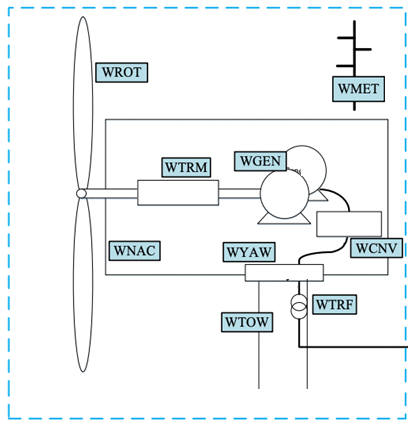
\includegraphics[width=7cm]{Resim/Sekil4-1.png}}
\caption{IEC 61400 standardına göre Türbin içerisindeki  algılayıcı düğümlerin gösterimi (\protect\citeA{jannasch2009daten}).}
\label{fig:figure15}
\end{figure}

\gls{iec} 61850 ve \gls{iec} 61400 standartları dikkate alındığında bir rüzgar türbininin sağlıklı bir şekilde çalışması için üzerinde faal durumda olması gereken 79 analog, 32 adet durum algılayıcısı bulunmalıdır. Tablo \ref{tab:tabb2}’de bir rüzgar türbininde bulunan algılayıcıların sayıları ve bağlı oldukları modüller gösterilmiştir. Tablo \ref{tab:WNACdetay}’de türbin içi modüllerden \gls{wnac}, rüzgar türbinlerinin pal kısmını kapsayan motor mekanizmasına ait modüldür. Bu modüle ait 4 durum ve 11 adet analog algılayıcı bulunmaktadır. WNAC modülüne ait algılayıcıların yerleşim detayı Şekil \ref{fig:4-2}'de, algılayıcıların tanımı ise Tablo \ref{tab:WNACdetay}’de gösterilmiştir. 
\cite{francisco2016protection}\cite{trinnass}\cite{san2007use}.


\begin{table}[htbp]
\centering
\caption{Türbin içi mantıksal düğüm özellikleri}
\label{tab:tabb2}
\begin{tabular}{ccccc}
\begin{tabular}[c]{@{}c@{}}Modül\\ İsmi\end{tabular} &
  \begin{tabular}[c]{@{}c@{}}Modül\\ Tanımı\end{tabular} &
  \begin{tabular}[c]{@{}c@{}}Zorunlu/\\ Opsiyonel\end{tabular} &
  \begin{tabular}[c]{@{}c@{}}Durum\\ Algılayıcı\\ Sayısı\end{tabular} &
  \begin{tabular}[c]{@{}c@{}}Analog\\ Algılayıcı\\ Sayısı\end{tabular} \\ \hline
WROT & Türbin rotor modülü       & Zorunlu   & 5 & 12 \\
WTRM & Türbin şanzıman modülü    & Opsiyonel & 8 & 12 \\
WGEN & Türbin jeneratör modülü   & Zorunlu   & 2 & 14 \\
WCNV & Türbin dönüştürücü modülü & Opsiyonel & 2 & 15 \\
WTRF & Türbin trafo modülü       & Opsiyonel & 3 & 8  \\
\gls{wnac} & Türbin motor modülü       & Zorunlu   & 4 & 11 \\
WYAW & Türbin yön ve açı modülü  & Zorunlu   & 2 & 6  \\
WTOW & Türbin kule modülü        & Opsiyonel & 3 & 2  \\
WMET & Türbin meteoroloji modülü & Zorunlu   & 0 & 8 
\end{tabular}
\end{table}


\begin{table}[htbp]
\centering
\caption{\gls{wnac} modülüne ait algılayıcıların tanımı \gls{iec} 61400-25 std.}
\label{tab:WNACdetay}
\begin{tabular}{ll}
\multicolumn{2}{l}{Durum algılayıcıları}        \\ \hline
BecBulbSt & İndikatör                           \\
WdHtSt    & Rüzgar algılayıcı ısıtıcı durumu    \\
IceSt     & Buz algılayıcı durumu               \\
AveSt     & Birinci ve ikinci anemometre durumu \\
\multicolumn{2}{l}{Analog algılayıcıları}           \\ \hline
Dir       & Türbin pal yönü                     \\
WdSpd     & Motor dışı rüzgar hızı              \\
WdDir     & Motor dışı rüzgar yönü              \\
ExTmp     & Modor dış sıcaklığı                 \\
IntlTmp   & Motor iç sıcaklığı                  \\
IntlHum   & Motor iç nemi                       \\
BecLumLev & Uyarı ışığı lüks değeri             \\
Vis       & Motor dışı görüş netlik değeri      \\
Ice       & Buz kalınlığı                       \\
DispXdis  & Kule yön değişikliği yatay açı      \\
DispYdir  & Kule yön değişikliği dikey açı      \\ \hline
\end{tabular}
\end{table}


\subsection{Güneş Enerji Sistemlerinde Veri Yapıları}
Güneş enerji sistemlerinde üretilen enerjinin takibi ve kontrolü için \gls{iec} 61724 standardı oluşturulmuştur. İlgili standardın amacı;

•	Fotovoltaik sistemdeki performans trendlerinin belirlenmesi.

•	Fotovoltaik sistemdeki olası arızaların lokalizasyonu.

•	Fotovoltaik sistem performansının tasarım beklentileri ve garantileriyle karşı-laştırılması.

•	Farklı konfigürasyonlardaki fotovoltaik sistemlerin karşılaştırılması.

•	Farklı lokasyonlardaki fotovoltaik sistemlerin karşılaştırılması 
olarak tanımla-nabilir. \cite{klise2017application} \cite{iec_2019} 

Bahsedilen amaçlar doğrultusunda tasarlanan güneş enerji sistemlerinde, performans analizlerinin yapılması hataların kolayca tespit edilmesi ve benzeri bir çok görevin başarıyla tamamlanmasına imkan vermektedir. \gls{iec} 61724 standardına göre izleme sistemi, güneş enerjisi sisteminin boyutuna ve kullanıcı gereksinimlerine göre uyarlanması gerektiğini belirtir \cite{trinnass}.

Genel olarak, daha büyük ve daha pahalı \gls{ges}, daha küçük ve daha düşük mali-yetli güneş enerjisi sistemlerinden daha fazla izleme noktasına ve daha yüksek doğrulukta algılayıcılara sahip olmalıdır. Bu gereksinime göre güneş enerji sistemleri A sınıfı, B sınıfı ve C sınıfı olarak üç sınıfta incelenir. Güneş enerji sistemlerinde çalışan algılayı-cıların genel olarak örnekleme ve veri gönderme periyotlarının maksimum değerleri Tablo \ref{tab:tablo4-3}’de gösterilmiştir.


\begin{table}[htbp]
\centering
\caption{Güneş tarlasında kullanılan algılayıcıların özellikleri}
\label{tab:tablo4-3}
\begin{tabular}{lccc}
Algılayıcı sınıfları &
  \multicolumn{1}{l}{\begin{tabular}[c]{@{}l@{}}A sınıfı (Yüksek\\ tutarlılık periyodu)\end{tabular}} &
  \multicolumn{1}{l}{\begin{tabular}[c]{@{}l@{}}B sınıfı (Orta\\ tutarlılık periyodu)\end{tabular}} &
  \multicolumn{1}{l}{\begin{tabular}[c]{@{}l@{}}C sınıfı (Düşük\\ tutarlılık periyodu)\end{tabular}} \\ \hline
Radyant ışıma        & 3s  & 60s & 60s \\
Meteorolojik         & 3s  & 60s & 60s \\
Rüzgar değerleri     & 3s  & 60s & 60s \\
Elektriksel değerler & 3s  & 60s & 60s \\
Kirlenme değerleri   & 60s & 60s & 60s
\end{tabular}
\end{table}


Tablo \ref{tab:tablo4-3}’de gösterilen algılayıcı sınıflarından yola çıkılarak 2015 senesinde yazılan bir makalede küçük çaplı güneş enerji sistemlerinde kullanılan algılayıcıların haber-leşme analizi yapılmıştır. \cite{ahmed2015communication}

\section{OPNET Yazılımı}

Günümüzde \gls{iot} ve veri haberleşmesinin boyutlarının her geçen gün artması nedeniyle şirketlerin haberleşme sistemlerine yapmış olduğu yatırımların büyüklüğü artmakta olduğu bilinmektedir. Haberleşme çözümleri için kullanılan donanımların sayısı arttıkça kurulum maliyeti ve sistemsel bir aksamanın oluşturacağı maliyet orantılı bir şekilde artacaktır. Buna göre araştırmacılar bir haberleşme sisteminin sahada kurulum aşamasından önce simülasyon ortamında tasarlanarak ilgili maliyetlerin fizibilitesini yapabilecekleri yazılımlar tasarlamışlardır. \gls{opnet} şimdiye kadar tasarlanmış en popüler ağ simülatör yazılımıdır. \gls{opnet} ticari bir yazılımdır ve ticari amaçlarla kullanılmasından kaynaklı olarak, OPNET hakkında yazılmış çok fazla makale ve kitap bulunmaktadır \cite{lu2012unlocking}\cite{sethi2012practical}. 

\begin{comment}
\subsection{OPNET Yazılımının Özellikleri}

•	Kolay bir grafik arayüzüne sahiptir.

•	Kullanıcılara zengin bir ağ modeli ve ağ tasarım kütüphanesi sunmaktadır.

•	Kullanıcı kolayca senaryo analizi yapabilmektedir.

•	Kurulumu diğer ağ tasarım programlarına göre daha kolaydır.

•	Grafik arayüzleri sayesinde sanal gerçek zamanlı ortam sağlar.

•	Ticari bir program olmasından kaynaklı, güvenilir ve verimlidir.

\end{comment}




\subsection{OPNET Yazılımında Algılayıcı Düğümlerin Modellenmesi}

Rüzgar türbinlerinde ve güneş enerjisi tarlalarında gözlem ve durum analizinin kolayca uygulanması için bir takım algılayıcı modüller \gls{iec} 61400, \gls{iec} 61724 ve \gls{iec} 61850 standartlarına göre oluşturulmuştur\cite{ahmed2011simulation}. \gls{iec} 61400 standardı dikkate alınarak bir rüzgar enerji türbininin OPNET yazılımında simülasyonu yapılmıştır. Bu çalışmada tasarlanan algılayıcı düğümlerinin Ethernet standartlarına göre haberleşme altyapısı oluşturulmuş 10BaseT, 100BaseT ve 1000BaseX standartlarındaki haberleşme hızlarına göre performansı incelenmiştir.
Kütahya Dumlupınar Üniversitesi'ndeki uzak yerleşkelere kurulacak güneş ve rüzgar enerji sistemlerindeki algılayıcıların tasarımında ilgili makalede bahsedilen teknikler kullanılmıştır. Şekil \ref{fig:4-2} ve Şekil \ref{fig:4-3} OPNET ortamında türbin içi ve MYO vaziyet planlarını göstermektedir. Tüm algılayıcı düğümler ilgili \gls{iec} standartları gereği bağlı oldukları sistemin çatısı altındaki kontrol sunucularına çalışma, durum ve ölçüm verilerini gönderirler. Algılayıcı düğümlerinin OPNET ortamında tasarımı dört değişken üzerinden yapılmıştır\cite{ahmed2011simulation}. Bunlar;

•	Örnekleme Frekansı

•	Başlama Zamanı

•	Bitiş Zamanı

•	Paket Boyutu

\begin{figure}[htbp]
\centerline{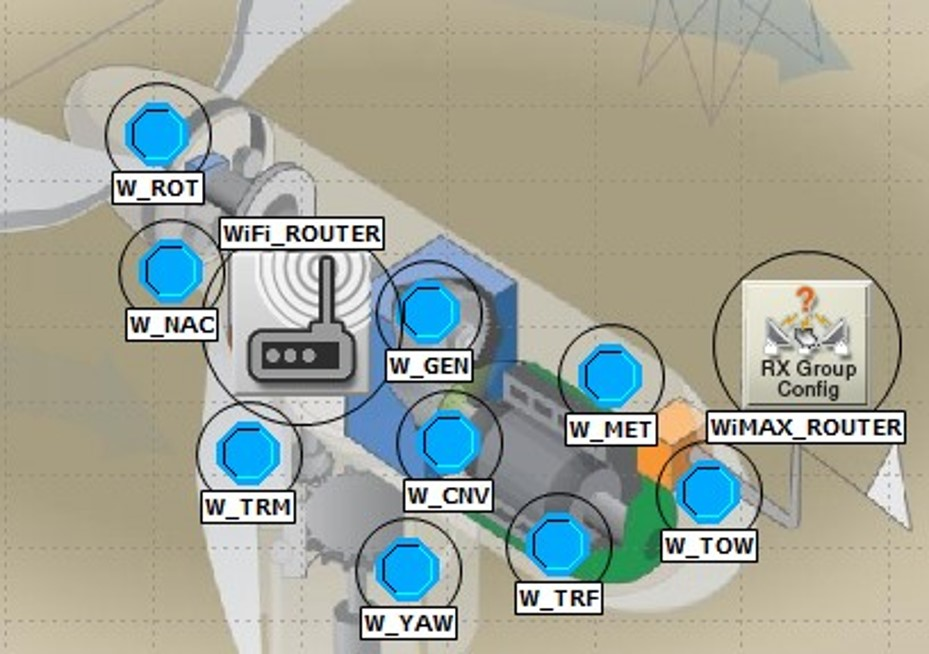
\includegraphics[width=8cm]{Resim/Wind_inside.jpg}}
\caption{Türbin içi \gls{wnac} modülünün temsili gösterimi.}
\label{fig:4-2}
\end{figure}


\begin{figure}[htbp]
\centerline{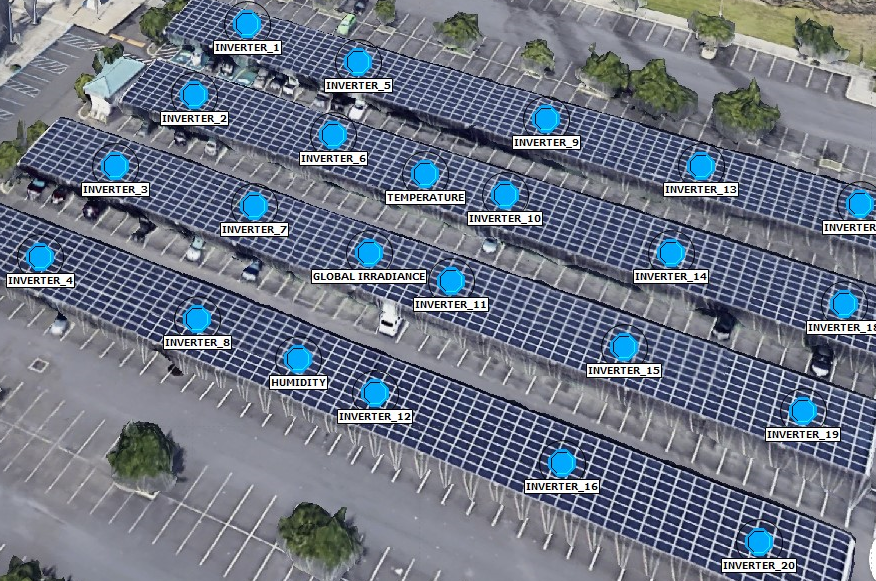
\includegraphics[width= 14cm]{Resim/mak2solar.png}}
\caption{OPNET yazılımında güneş enerji sisteminde çalışan algılayıcı modüllerin gösterimi}
\label{fig:4-3}
\end{figure}


\subsection{Algılayıcı Düğümlerin Veri Boyutu Hesaplanması}\label{verboyut}

Bu bölüm, rüzgar türbini ve güneş enerji tarlalarında durum izleme ve arıza tahmini görevlerini gerçekleştirmek için çalışan algılayıcı düğümlerinin oluşturduğu veri boyutlarını açıklamaktadır. İlgili algılayıcıların temel prensipleri 4.1.1 ve 4.1.2 başlıkla-rında açıklanmıştır.


Yenilenebilir enerji sistemlerinde çalışan algılayıcı düğümlerinin oluşturdukları veri boyutu Denklem \eqref{eq4-1} ile bulunabilir \cite{ahmed2011simulation}.


\begin{equation}
\text{Veri hızı} = 2.\text{f\textsubscript{s}} \label{eq4-1}
\end{equation}

Mantıksal düğümler 2 Byte’lık veri üretecek şekilde tasarlanmıştır. Örnekleme frekansı (\text{f\textsubscript{s}}) ile çarpılarak bir saniyede oluşturduğu veri boyutu hesaplanmış olur. Çalışan sisteme ait üretilen veri boyutlarının OPNET ortamına uyarlanma imkanı sağlanmaktadır. Denklem \eqref{eq4-1}'den faydalanılarak \gls{res} ve \gls{ges} içerisinde çalışan algılayıcıların 1 saniyede oluşturduğu veri boyutları değişimi Tablo \ref{tab:tablo4-4} ve Tablo \ref{tab:tablo4-5}’te gösterilmiştir \cite{klise2017application}.


\begin{table}[htbp]
\centering
\caption{Rüzgar türbinindeki algılayıcı gruplarının ürettiği veri boyutları}
\label{tab:tablo4-4}
\begin{tabular}{cccc}
\multicolumn{1}{c}{\begin{tabular}[c]{@{}c@{}}Algılayıcı modül\\ isimleri\end{tabular}} &
  \begin{tabular}[c]{@{}c@{}}Durum algılayıcı\\ veri boyutu (f\textsubscript{s} = 1)\end{tabular} &
  \begin{tabular}[c]{@{}c@{}}Analog algılayıcı\\ veri boyutu (f\textsubscript{s} = 500)\end{tabular} &
  \begin{tabular}[c]{@{}c@{}}Toplam aktarılan\\ veri\end{tabular} \\ \hline
WROT & 5*2*f\textsubscript{s} = 10 Byte/s & 12*2*f\textsubscript{s} = 12000 Byte/s     & 12010 Byte/s \\
WTRM & 8*2*f\textsubscript{s} = 16 Byte/s & 12*2*f\textsubscript{s} = 12000 Byte/s  & 12016 Byte/s \\
WGEN & 2*2*f\textsubscript{s} = 4 Byte/s  & 14*2*f\textsubscript{s} = 14000 Byte/s & 14004 Byte/s \\
WCNV & 2*2*f\textsubscript{s} = 4 Byte/s  & 15*2*f\textsubscript{s} = 15000 Byte/s & 15004 Byte/s \\
WTRF & 3*2*f\textsubscript{s} = 6 Byte/s  & 8*2*f\textsubscript{s} = 8000 Byte/s   & 8006 Byte/s  \\
\gls{wnac} & 4*2*f\textsubscript{s} = 8 Byte/s  & 11*2*f\textsubscript{s} = 11000 Byte/s & 11008 Byte/s \\
WYAW & 2*2*f\textsubscript{s} = 4 Byte/s  & 6*2*f\textsubscript{s} = 6000 Byte/s   & 6004 Byte/s  \\
WTOW & 3*2*f\textsubscript{s} = 6 Byte/s  & 2*2*f\textsubscript{s} = 2000 Byte/s   & 2006 Byte/s  \\
WMET & 0                  & 8*2*f\textsubscript{s}= 8000 Byte/s    & 8000 Byte/s 
\end{tabular}
\end{table}

Tablo \ref{tab:tablo4-4}'e göre rüzgar türbinindeki algılayıcı düğümlerinin yapısı için OPNET yazılımında “Application config” modülü eklenerek \gls{iec} 61400-25 ve \gls{iec} 61724 standartlarına göre ANALOG ve STATUS verileri Şekil \ref{fig:4-4}'teki gibi oluşturulur.“Application config” modülünde tasarlanan uygulama verilerinin, ağ senaryolarında kullanılması için “Profil Definition” modülüne entegre edilmesi gerekir. 

\begin{table}[htbp]
\centering
\caption{Güneş enerji tarlasındaki algılayıcı gruplarının ürettiği veri boyutları}
\label{tab:tablo4-5}
\begin{tabular}{lc}
\multicolumn{1}{c}{\begin{tabular}[c]{@{}c@{}}Algılayıcı modül isimleri\end{tabular}} & A sınıfı (yüksek tutarlılık periyodu) \\ \hline
Radyant ışıma              & 1*2*100 = 200 Byte/s    \\
Meteoroloji modülü               & 5*2*1 = 10 Byte/s       \\
Rüzgar hızı                & 1*2*3 = 6 Byte/s        \\
İnverter (Gerilim ve Akım) & 2*2*1440 = 28800 Byte/s
\end{tabular}
\end{table}

\begin{figure}[htbp]
\centerline{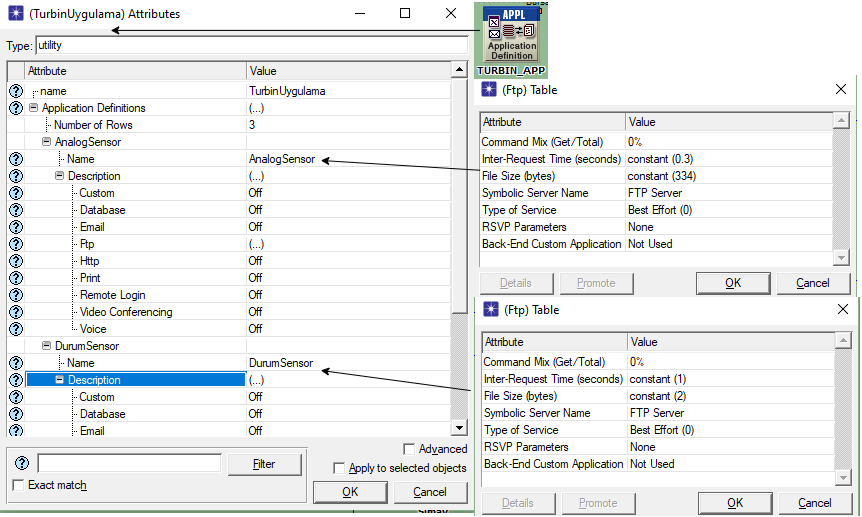
\includegraphics[width=13.5cm]{Resim/sekil4-4.png}}
\caption{OPNET Yazılımında “Application Config” bölümü}
\label{fig:4-4}
\end{figure}

Örneğin, invertör profiline ait güneş panelinde voltaj ve akım algılayıcısı olarak iki adet algılayıcı modeli bulunmaktadır. Bu kritere göre OPNET yazılımının “Application Config” modülünde gerilim ve akım algılayıcılarının veri boyutları oluşturulur. İkinci aşamada ise oluşturulan bu veri boyutları “Profil Definition” modülü kullanılarak invertör profili çatısında toplanır. Böylelikle tasarlanan invertör, OPNET’in ağ senaryolarında kullanımı sağlanmış olur. Şekil \ref{fig:4-5}’te \gls{wnac} profilinin \gls{opnet} yazılım yapısı gösterilmiştir. Tablo \ref{tab:tablo4-4}’e göre \gls{wnac}'a ait olan algılayıcılar \gls{opnet} yazılımında kurulmuştur. Rüzgar türbininde enerji üretimi gerçekleşirken eş zamanlı çalışan \gls{wnac} gibi toplamda 9 adet algılayıcı düğüm modül grubu, güneş enerji sisteminde kullanılan 4 adet algılayıcı düğüm modül grubu, “Application config” ve “Profile config” bileşenleri kullanılarak simülasyon ortamında çalışan algılayıcı gruplarına dönüştürülmüştür.
\begin{figure}[htbp]
\centerline{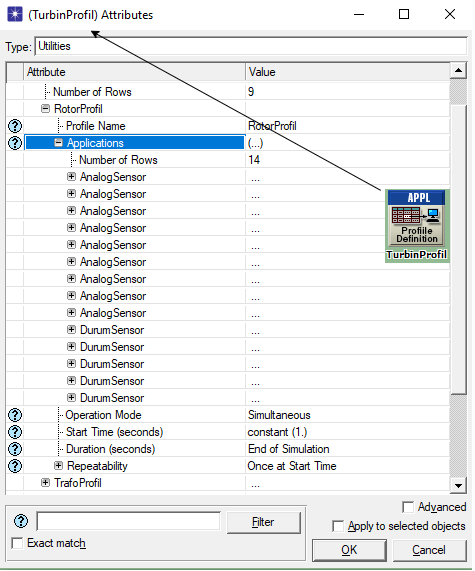
\includegraphics[width=8cm]{Resim/sekil4-5.png}}
\caption{OPNET Yazılımında “Profile Definition" bölümü}
\label{fig:4-5}
\end{figure}

\part{DAĞITIK ALGILAYICI AĞI TASARIM VE SİMÜLASYON SONUÇLARI}


%\part{OPNET İLE YENİLENEBİLİR ENERJİ SİSTEMİ İÇİN DAĞITIK SENSÖR AĞI TASARIM VE SİMÜLASYON SONUÇLARI}
\thispagestyle{empty}
\newpage
\section{LAN TASARIM VE SİMÜLASYON SONUÇLARI}
\subsection{OPNET Yerel Ağ Tasarımı} \label{opnetges}

\begin{figure}[htbp]
\centerline{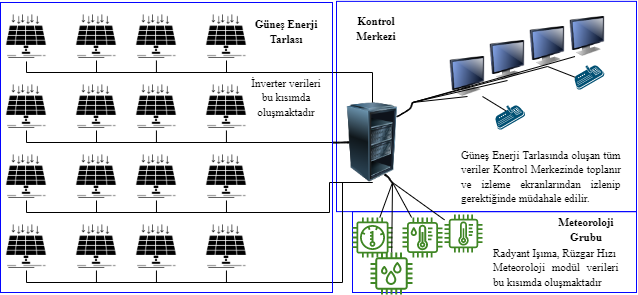
\includegraphics[width=\columnwidth]{Resim/PV-2.png}}
\caption{Güneş enerji sistemi haberleşme topolojisi}
\label{fig:4-6}
\end{figure}

Şekil \ref{fig:4-6}’da sahada kurulu olarak çalışan güneş enerji panelleri ve hava durumu algılayıcılarının sistem odasında bulunan sunucuyla bağlantısı ve sunucu ile komuta kontrol merkezinde bulunan görüntüleme bilgisayarları arasındaki bağlantının topolojisi gösterilmiştir. İlgili topoloji sadece yerel ağı gösteren bir topoloji olduğu unutulmamalıdır. \gls{wan} tasarımı hakkında yapılan çalışmalar, ayrı bir başlıkta incelenmiştir.

\subsubsection{Ethernet Teknolojisi \gls{lan} Tasarımı}\label{yerelEthernet}


\paragraph{Güneş Enerji Sistemi \gls{lan} Tasarımı }

\begin{figure}[htbp]
\centerline{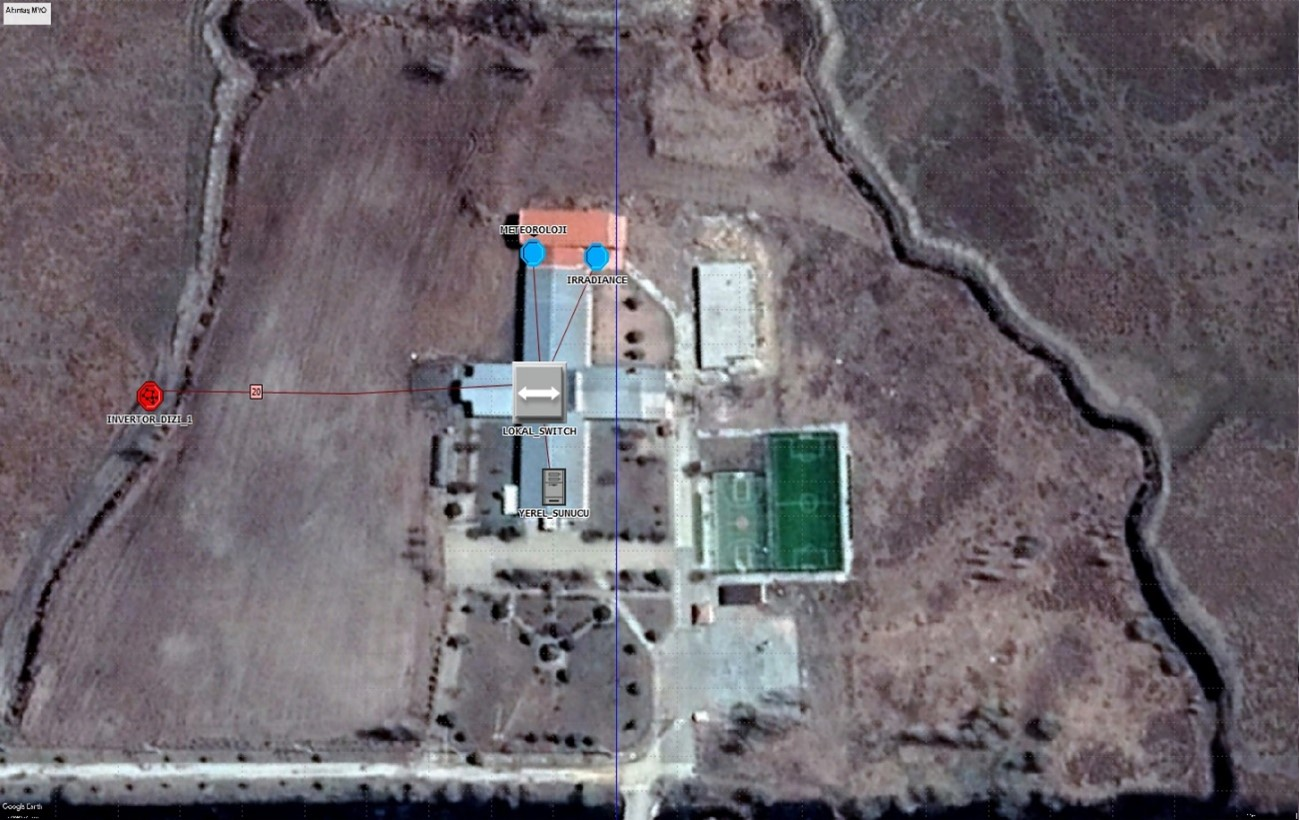
\includegraphics[width=\columnwidth]{Resim/Sekil4-7.jpg}}
\caption{Altıntaş \gls{myo}'nun OPNET yazılımda tasarım topolojisi.}
\label{fig:4-7}
\end{figure}

Bölüm \ref{opnetges}'deki ilgili tabloda güneş enerji sisteminde kullanılan algılayıcılara göre OPNET yazılımında oluşturulan ağın görseli Şekil \ref{fig:figure9}'dedir. İlgili ağ yapısının tasarımı için OPNET yazılımında seçilmiş Ethernet algılayıcı düğümünün detayı şekil \ref{fig:4-9}’da gösterilmiştir. Bölüm \ref{algilayicidugum}'de tanımlanan Ethernet düğüm modülü ile OPNET yazılımında düğüm modülü uyumluluk göstermektedir.

Yerel enerji üretim durumunu kontrol edebilmek için komuta kontrol merkezi ile enerji üretim sisteminin haberleşme gecikmesinin 1 saniyenin altında olması ve paket trafiğinin minimum gecikmeyle komuta merkezine aktarılması gerektiği \gls{iec} 61724 standardının temel kriteridir. Bu kritere göre tasarlanan topolojide gözlemlenen performans değerleri Şekil \ref{fig:4-10}--\ref{fig:4-12}’lerde paylaşılmıştır.


\begin{figure}[htbp]
\centerline{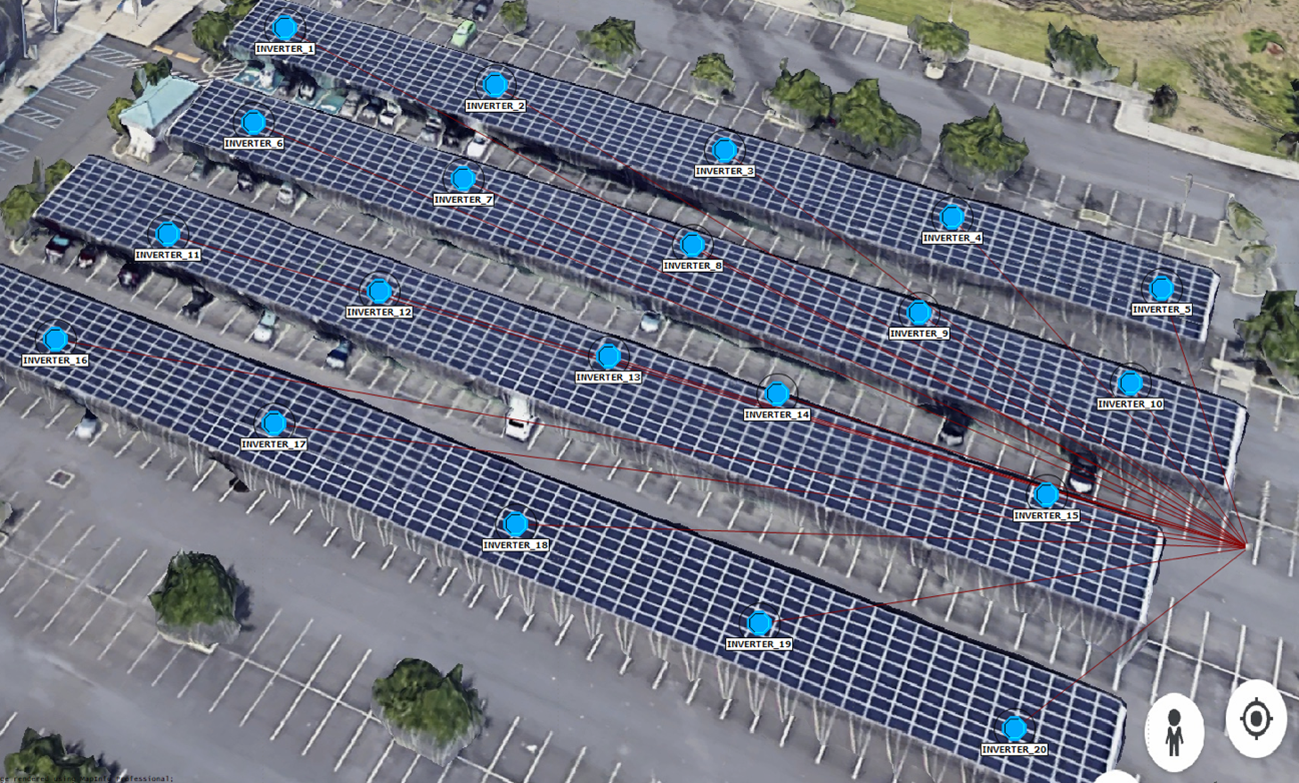
\includegraphics[width=10cm]{Resim/Sekil 4-8.png}}
\caption{Kampüs ortamında kurulan örnek güneş enerji santralinin invertör dizi grubunun OPNET yazılımında tasarlanması.}
\label{fig:4-8}
\end{figure}

\begin{figure}[htbp]


\centerline{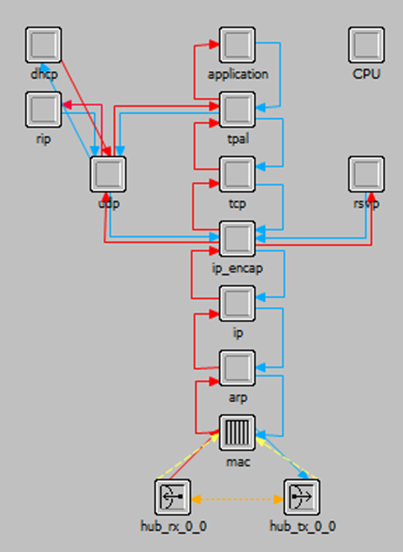
\includegraphics[width=7cm]{Resim/Sekil4-9.png}}
\caption{OPNET yazılımında tasarlanan ethernet tipi algılayıcıların görüntüsü. Algılayıcı düğümlerde oluşturulan ölçüm ve durum verileri IP haberleşme standardına geçebilmesi için gereken işleç grupları görülmektedir. İlgili ölçüm ve durum veri paketlerinin önüne veya sonuna eklenen paketler sayesinde haberleşme sisteminde rotalama işlemleri yapılmaktadır.}
\label{fig:4-9}
\end{figure}
\begin{comment}
%ESKİ ŞEKİL SİLEBİLİRSİN
\begin{figure}[htbp]
\centerline{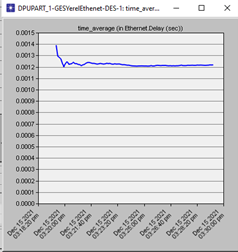
\includegraphics[width=5cm]{Resim/sekil4-10.png}}
\caption{\gls{lan}'da ethernet haberleşmesinde gözlemlenen gecikme değişimi.}
\label{fig:4-10}
\end{figure}
\end{comment}



\begin{figure}[htbp]
\centering
%ethernet haberleşmesinde LAN gecikme grafiğidir
\pgfplotsset{every axis/.append style={
font=\footnotesize,
thin,
tick style={ultra thin}},
scaled y ticks=false,
yticklabel style = {
/pgf/number format/fixed,
/pgf/number format/precision=5
},
}

    \begin{tikzpicture}
    \begin{axis}[
    xlabel={Simülasyon Süresi (Saniye)},
    ylabel={Uçtan Uca Gecikme (Saniye)},
    grid,
    legend style = {font=\tiny,at={(1,0.8)}, anchor=east}
    ]

\addplot [color=cyan, mark=star, mark repeat =14, mark size = 3]  table [x = timesec, y = GESYerelEthenetEthernetDelaysec, col sep = comma] {yedek.csv};
%\addlegendentry{Ethernet bağlantı gecikme değeri}



\end{axis}
\end{tikzpicture}
\caption{\gls{lan}'da ethernet haberleşmesinde gözlemlenen gecikme değişimi.}
\label{fig:4-10}
\end{figure}




\begin{comment}

\begin{figure}[htbp]
\centerline{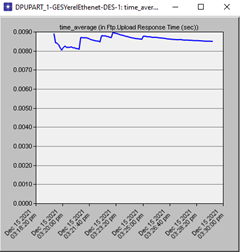
\includegraphics[width=5cm]{Resim/sekil4-11.png}}
\caption{\gls{lan}'da algılayıcılardan gönderilen verilerin yerel sunucuya yüklenme süresi}
\label{fig:4-11}
\end{figure}
\end{comment}

\begin{figure}[htbp]


\centering
%ethernet haberleşmesinde LAN gecikme grafiğidir
\pgfplotsset{every axis/.append style={
font=\footnotesize,
thin,
tick style={ultra thin}},
scaled y ticks=false,
yticklabel style = {
/pgf/number format/fixed,
/pgf/number format/precision=5
},
}

    \begin{tikzpicture}
    \begin{axis}[
    ylabel={Veri Yükleme Süresi (Saniye)},
    xlabel={Simülasyon Süresi (Saniye)},
    grid,
    legend style = {font=\tiny,at={(1,0.8)}, anchor=east}
    ]

\addplot [color=red, mark=star, mark repeat =14, mark size = 3]  table [x = timesec, y = GESYerelEthenetFtpUploadResponseTimesec, col sep = comma] {yedek.csv};
%\addlegendentry{Ethernet bağlantı gecikme değeri}



\end{axis}
\end{tikzpicture}


\caption{\gls{lan}'da algılayıcılardan gönderilen verilerin yerel sunucuya yüklenme süresi değişimi.}
\label{fig:4-11}
\end{figure}



\begin{figure}[htbp]
%\centerline{\includegraphics[width=5cm]{Resim/şekil4-12.png}}
\centering
\pgfplotsset{every axis/.append style={
font=\footnotesize,
thin,
tick style={ultra thin}},
}
    \begin{tikzpicture}
\begin{semilogyaxis}[ymax = 20000.0000000,
xlabel={Simülasyon Süresi (Saniye)},
ylabel={Yüklenen Veri Boyutu (Byte/s)},
xmode=normal, ymode=log, 
grid = major,
log ticks with fixed point,
ytick={6,10,200,14400},
transpose legend,
legend columns = 2,
legend style = {font=\tiny,at={(1,0.8)}, anchor=east}
]


\addplot [color=blue, mark=oplus*, mark repeat =14, mark size = 3]  table [x = Simulation Duration, y = Received Current Data, col sep = comma] {fig4deneme (1).csv};


%--
\addplot [color=yellow, mark=pentagon*, mark repeat =14, mark size = 3, mark phase = 8]  table [y = Received Voltage Data, col sep = comma] {fig4deneme (1).csv};

%--

\addplot [color = green, dotted, mark=diamond*, mark repeat =14, mark size = 3, ]table [y = METEOR, col sep = comma] {fig4deneme (1).csv};

%--
\addplot [color=orange, mark=square*, mark repeat =14, mark size = 3]table [y = Received Wind Speed Data, col sep = comma] {fig4deneme (1).csv};

%---
\addplot [color=violet, mark=triangle*, mark repeat =14, mark size = 3] table [y = Received Global Irradiance Data, col sep = comma] {fig4deneme (1).csv};


\legend{İnverter Gerilim,İnverter Akım,Rüzgar Hızı,Meteoroloji,Radyant Işıma}


\end{semilogyaxis}
\end{tikzpicture}
\caption{\gls{lan}'da 1 adet \gls{myo}'ya ait yerel sunucuya yüklenen veri grubunun değişimi.}
\label{fig:4-12}
\end{figure}




\newpage


\paragraph{Rüzgar Enerji Sistemi LAN Tasarımı}

Ethernet haberleşmesinde \gls{utp} kablolamanın en büyük sıkıntısı mesafedir. 
Veri aktarımında 100 metrede 24,6dB güç kaybı olmasından dolayı mutlaka cihaz aralarına güçlendirici kullanılması gerekir \cite{yilmazanalysis}. Tezde model olarak kullanılan rüzgar türbinlerinin yüksekliği 80 metredir \cite{bauer_2010}.
Algılayıcı düğüm modüllerinden gelen Ethernet kabloları türbinin zemininde bulunan bir toplayıcı anahtara gelmektedir. Toplayıcı anahtar ile lokal sunucunun olduğu komuta merkezindeki yönetim anahtarına \gls{utp} kablo bağlantısı vardır. Farklı kablo altyapıları kullanılarak haberleşme sağlanabilir örnek olarak fiber optik kablosu seçildiğinde optik kablo için Ethernet anahtarı arasına konulacak bir fiber dönüştürücü modül ve fiber kablolarının füzyon eki ile sonlandırma kutusu ve yan ekipmanlarına ihtiyaç duyulacaktır. Bu tasarımın getireceği ekstra malzemeler bir maliyet unsuru oluşturacağından sadece \gls{utp} kablolama ile çözüme gidilme tercihi kabul edilmiştir.

\begin{figure}[htbp]
%\centerline{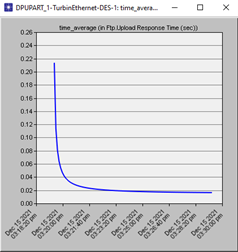
\includegraphics[width=6cm]{Resim/sekil4-13.png}}
\centering
%ethernet haberleşmesinde LAN gecikme grafiğidir
\pgfplotsset{every axis/.append style={
font=\footnotesize,
thin,
tick style={ultra thin}},
scaled y ticks=false,
yticklabel style = {
/pgf/number format/fixed,
/pgf/number format/precision=5
},
}

    \begin{tikzpicture}
    \begin{axis}[
    xlabel={Simülasyon süresi (Saniye)},
    ylabel={Veri Yükleme Süresi (Saniye)},
    grid,
    legend style = {font=\tiny,at={(1,0.8)}, anchor=east}
    ]

\addplot [color=red, mark=star, mark repeat =14, mark size = 3]  table [x = Simulation Duration, y = TurbinUploadResponseTime, col sep = comma] {fig4deneme (1).csv};
%\addlegendentry{Ethernet bağlantı gecikme değeri}



\end{axis}
\end{tikzpicture}


\caption{Algılayıcılardan gönderilen verilerin \gls{lan} sunucuya yüklenme süre değişimi.}
\label{fig:4-13}
\end{figure}


\begin{figure}[htbp]
%\centerline{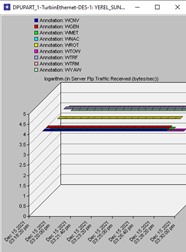
\includegraphics[width=5cm]{Resim/sekil4-14.png}}

\centering
\pgfplotsset{every axis/.append style={
font=\footnotesize,
thin,
tick style={ultra thin}},
}
    \begin{tikzpicture}
\begin{semilogyaxis}[ymax = 20000.0000000,
xlabel={Simülasyon Süresi (Saniye)},
ylabel={Yüklenen Veri Boyutu (Byte/s)},
xmode=normal, ymode=log, 
grid = major,
log ticks with fixed point,
ytick={15004,14004,8000,11008,12010,2006,8006,12016,6004},
transpose legend,
legend columns = 3,
legend style = {font=\tiny,at={(1,0.3)}, anchor=east}
]


\addplot [color=blue, mark=oplus*, mark repeat =14, mark size = 3]  table [x = Simulation Duration, y = WCNV, col sep = comma] {fig4deneme (1).csv};


%--
\addplot [color=yellow, mark=pentagon*, mark repeat =14, mark size = 3, mark phase = 8]  table [y = WGEN, col sep = comma] {fig4deneme (1).csv};

%--

\addplot [color = green, dotted, mark=diamond*, mark repeat =14, mark size = 3, ]table [y = WMET, col sep = comma] {fig4deneme (1).csv};

%--
\addplot [color=orange, mark=square*, mark repeat =14, mark size = 3]table [y = WNAC, col sep = comma] {fig4deneme (1).csv};

%---
\addplot [color=violet, mark=triangle*, mark repeat =14, mark size = 3] table [y = WROT, col sep = comma] {fig4deneme (1).csv};

%--
\addplot [color=yellow, mark=pentagon*, mark repeat =14, mark size = 3, mark phase = 8]  table [y = WTOW, col sep = comma] {fig4deneme (1).csv};


%--
\addplot [color=black, mark=pentagon*, mark repeat =14, mark size = 1, mark phase = 8]  table [y = WTRF, col sep = comma] {fig4deneme (1).csv};

%--
\addplot [color=orange, mark=pentagon*, mark repeat =14, mark size = 1, mark phase = 8]  table [y = WTRM, col sep = comma] {fig4deneme (1).csv};


%--
\addplot [color=cyan, mark=pentagon*, mark repeat =14, mark size = 1, mark phase = 8]  table [y = WYAW, col sep = comma] {fig4deneme (1).csv};
\legend{WCNV , WGEN , WMET , WNAC , WROT , WTOW , WTRF , WTRM , WYAW}
\end{semilogyaxis}



\end{tikzpicture}



\caption{\gls{lan} sunucusuna yüklenen veri grubunun logaritmik eksende zamana bağlı değişim grafiği.}
\label{fig:4-14}
\end{figure}

\begin{figure}[htbp]
%\centerline{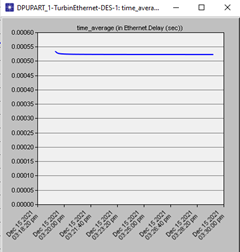
\includegraphics[width=5cm]{Resim/sekil4-15.png}}

\centering
%ethernet haberleşmesinde LAN gecikme grafiğidir
\pgfplotsset{every axis/.append style={
font=\footnotesize,
thin,
tick style={ultra thin}},
scaled y ticks=false,
yticklabel style = {
/pgf/number format/fixed,
/pgf/number format/precision=5
},
}

    \begin{tikzpicture}
    \begin{axis}[
    xlabel={Simülasyon Süresi (Saniye)},
    ylabel={Uçtan Uca Gecikme (Saniye)},
    grid,
    legend style = {font=\tiny,at={(1,0.8)}, anchor=east}
    ]

\addplot [color=red, mark=star, mark repeat =14, mark size = 3]  table [x = Simulation Duration, y = turbinEthernetDelay, col sep = comma] {fig4deneme (1).csv};
%\addlegendentry{Ethernet bağlantı gecikme değeri}



\end{axis}
\end{tikzpicture}
\caption{\gls{lan} senaryosunda ethernet sistemindeki yaşanan gecikmenin zamana bağlı değişim grafiği.}
\label{fig:4-15}
\end{figure}

Yerel enerji üretim durumunu kontrol edebilmek için komuta kontrol merkezi ile enerji üretim sisteminin haberleşme gecikmesinin 1 saniyenin altında olması ve paket trafiğinin minimum gecikmeyle komuta merkezine aktarılması gerektiği \gls{iec} 61400-25 standardının temel kriteridir. Bu kritere göre tasarlanan topolojinin performans değerleri Şekil \ref{fig:4-13}--\ref{fig:4-15}’de paylaşılmıştır.
\newpage  %BUNUN AMACI SAYFAYI DÜZGÜN ÇIKARTMAK İÇİN ÇÜNKÜ BAŞKA BİR SECTİON'UN ALTINDA ÖNCEKİ SECTİONA AİT RESİMLERİ ÇIKARTIYORDU
\subsubsection{\gls{wifi} Teknolojisi \gls{lan} Tasarımı}\label{yerelWifi}

\paragraph{Güneş Enerji Sistemi \gls{lan} Tasarımı}

\gls{wifi} altyapısında \gls{ges}'in maliyet ve performans değerleri ile Altıntaş \gls{myo}’nun OPNET ortamında simülasyon raporları bu bölümde paylaşılmıştır.


\begin{figure}[htbp]
\centerline{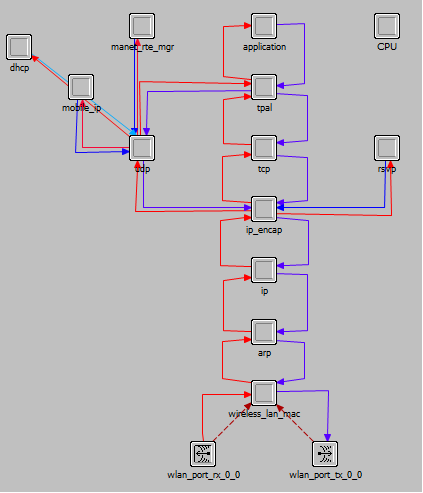
\includegraphics[width=7cm]{Resim/PV-Sayfa -5.drawio.png}}
\caption{OPNET yazılımındaki \gls{wifi} algılayıcı düğümünün gösterimi. Algılayıcı düğümlerde oluşturulan ölçüm ve durum verileri IP haberleşme standardına geçebilmesi için gereken işleç grupları görülmektedir. İlgili ölçüm ve durum veri paketlerinin önüne veya sonuna eklenen paketler sayesinde haberleşme sisteminde rotalama işlemleri yapılmaktadır.}
\label{fig:4-16}
\end{figure}


Yerel enerji üretim durumunu kontrol edebilmek için komuta kontrol merkezi ile enerji üretim sisteminin haberleşme gecikmesinin 1 saniyenin altında olması ve paket trafiğinin minimum gecikmeyle komuta merkezine aktarılması gerektiği \gls{iec} 61724 standardının temel kriteridir. Bu kritere göre tasarlanan topolojinin performans değerleri Şekil \ref{fig:4-17}--\ref{fig:4-19}’da paylaşılmıştır

\begin{figure}[htbp]
%\centerline{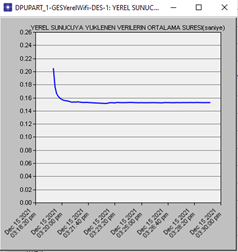
\includegraphics[width=5cm]{Resim/sekil4-16.png}}

\centering
%ethernet haberleşmesinde LAN gecikme grafiğidir
\pgfplotsset{every axis/.append style={
font=\footnotesize,
thin,
tick style={ultra thin}},
scaled y ticks=false,
yticklabel style = {
/pgf/number format/fixed,
/pgf/number format/precision=5
},
}

    \begin{tikzpicture}
    \begin{axis}[
    xlabel={Simülasyon süresi (Saniye)},
    ylabel={Veri Yükleme Süresi (Saniye)},
    grid,
    legend style = {font=\tiny,at={(1,0.8)}, anchor=east}
    ]

\addplot [color=red, mark=star, mark repeat =14, mark size = 3]  table [x = Simulation Duration, y = WifiYerelUploadTime, col sep = comma] {fig4deneme (1).csv};
%\addlegendentry{Ethernet bağlantı gecikme değeri}



\end{axis}
\end{tikzpicture}



\caption{\gls{lan}'da algılayıcılardan gönderilen verilerin yerel sunucuya yüklenme süresinin zaman bağlı değişim grafiği.}
\label{fig:4-17}
\end{figure}


\begin{figure}[htbp]
%\centerline{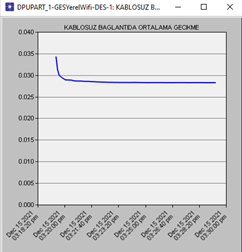
\includegraphics[width=5cm]{Resim/sekil4-17.png}}

\centering
%ethernet haberleşmesinde LAN gecikme grafiğidir
\pgfplotsset{every axis/.append style={
font=\footnotesize,
thin,
tick style={ultra thin}},
scaled y ticks=false,
yticklabel style = {
/pgf/number format/fixed,
/pgf/number format/precision=5
},
}

    \begin{tikzpicture}
    \begin{axis}[
    xlabel={Simülasyon Süresi (Saniye)},
    ylabel={Uçtan Uca Gecikme (Saniye)},
    grid,
    legend style = {font=\tiny,at={(1,0.8)}, anchor=east}
    ]

\addplot [color=cyan, mark=star, mark repeat =14, mark size = 3]  table [x = Simulation Duration, y = wirelessGESDelay, col sep = comma] {fig4deneme (1).csv};
%\addlegendentry{Ethernet bağlantı gecikme değeri}



\end{axis}
\end{tikzpicture}
\caption{\gls{lan} senaryosunda WiFi sistemindeki yaşanan gecikmenin zamana bağlı değişim grafiği.}
\label{fig:4-18}
\end{figure}

İlgili simülasyon sonuçlarına göre güneş enerji santralinin haberleşme standartlarında bir ihlal durumu olmadan sağlıklı bir şekilde yerel sunucuya verilerin aktarıldığı gözlemlenmiştir.

\begin{figure}[htbp]
%\centerline{\includegraphics[width=5cm]{Resim/Sekil4-18.png}}
\centering
\pgfplotsset{every axis/.append style={
font=\footnotesize,
thin,
tick style={ultra thin}},
}
    \begin{tikzpicture}
\begin{semilogyaxis}[ymax = 20000.0000000,
xlabel={Simülasyon Süresi (Saniye)},
ylabel={Yüklenen Veri Boyutu (Byte/s)},
xmode=normal, ymode=log, 
grid = major,
log ticks with fixed point,
ytick={6,10,200,14400},
transpose legend,
legend columns = 2,
legend style = {font=\tiny,at={(1,0.8)}, anchor=east}
]


\addplot [color=blue, mark=oplus*, mark repeat =14, mark size = 3]  table [x = Simulation Duration, y = INVERTERAKIMwifiges, col sep = comma] {fig4deneme (1).csv};


%--
\addplot [color=yellow, mark=pentagon*, mark repeat =14, mark size = 3, mark phase = 8]  table [y =INVERTERVOLTAJwifiges, col sep = comma] {fig4deneme (1).csv};

%--

\addplot [color = green, dotted, mark=diamond*, mark repeat =14, mark size = 3, ]table [y = METEORwifiges, col sep = comma] {fig4deneme (1).csv};

%--
\addplot [color=orange, mark=square*, mark repeat =14, mark size = 3]table [y = RUZGARHIZIwifiges, col sep = comma] {fig4deneme (1).csv};

%---
\addplot [color=violet, mark=triangle*, mark repeat =14, mark size = 3] table [y = RADYANTISIMAwifiges, col sep = comma] {fig4deneme (1).csv};


\legend{İnverter Gerilim,İnverter Akım,Rüzgar Hızı,Meteoroloji,Radyant Işıma}


\end{semilogyaxis}
\end{tikzpicture}


\caption{LAN’da 1 adet MYO’ya ait yerel sunucuya yüklenen veri grubunun logaritmik eksende zamana bağlı değişim grafiği.}
\label{fig:4-19}
\end{figure}
\newpage
\paragraph{Rüzgar Enerji Sistemi \gls{lan} Tasarımı}
Yerel enerji üretim durumunu kontrol edebilmek için komuta kontrol merkezi ile enerji üretim sisteminin haberleşme gecikmesinin 1 saniyenin altında olması ve paket trafiğinin minimum gecikmeyle komuta merkezine aktarılması gerektiği \gls{iec} 61400-24 standardının temel kriteridir. Domaniç \gls{myo}'nun rüzgar enerji sistemindeki haberleşme altyapısı \gls{wifi} olarak OPNET ortamında kurulduktan sonra edinilen simülasyon sonuçları Şekil \ref{fig:4-20}-\ref{fig:4-22}’de paylaşılmıştır.

\begin{figure}[htbp]
%\centerline{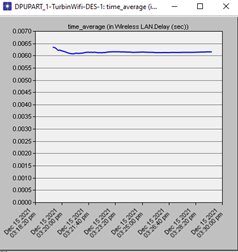
\includegraphics[width=5cm]{Resim/Sekil4-19.png}}


\centering
%ethernet haberleşmesinde LAN gecikme grafiğidir
\pgfplotsset{every axis/.append style={
font=\footnotesize,
thin,
tick style={ultra thin}},
scaled y ticks=false,
yticklabel style = {
/pgf/number format/fixed,
/pgf/number format/precision=5
},
}

    \begin{tikzpicture}
    \begin{axis}[
    xlabel={Simülasyon Süresi (Saniye)},
    ylabel={Uçtan Uca Gecikme (Saniye)},
    grid,
    legend style = {font=\tiny,at={(1,0.8)}, anchor=east}
    ]

\addplot [color=red, mark=star, mark repeat =14, mark size = 3]  table [x = Simulation Duration, y = WirelessLANDelaysecwifiLoc, col sep = comma] {fig4deneme (1).csv};
%\addlegendentry{Ethernet bağlantı gecikme değeri}



\end{axis}
\end{tikzpicture}


\caption{\gls{res}'in \gls{lan} senaryosunda WiFi sistemindeki yaşanan gecikmenin zamana bağlı değişim grafiği.}
\label{fig:4-20}
\end{figure}

\begin{figure}[htbp]
%\centerline{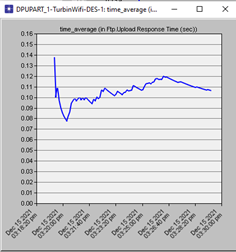
\includegraphics[width=5cm]{Resim/Sekil4-20.png}}

\centering
%ethernet haberleşmesinde LAN gecikme grafiğidir
\pgfplotsset{every axis/.append style={
font=\footnotesize,
thin,
tick style={ultra thin}},
scaled y ticks=false,
yticklabel style = {
/pgf/number format/fixed,
/pgf/number format/precision=5
},
}

    \begin{tikzpicture}
    \begin{axis}[
    xlabel={Simülasyon süresi (Saniye)},
    ylabel={Veri Yükleme Süresi (Saniye)},
    grid,
    legend style = {font=\tiny,at={(1,0.8)}, anchor=east}
    ]

\addplot [color=blue, mark=circle, mark repeat =14, mark size = 3]  table [x = Simulation Duration, y = FtpUploadResponseTimesecwifiLoc, col sep = comma] {fig4deneme (1).csv};
%\addlegendentry{Ethernet bağlantı gecikme değeri}



\end{axis}
\end{tikzpicture}


\caption{\gls{res}'in yerel sunucusuna yüklenen algılayıcı verilerinin zamana bağlı değişim grafiği.}
\label{fig:4-21}
\end{figure}


\begin{figure}[htbp]
%\centerline{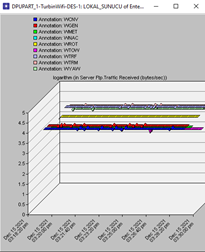
\includegraphics[width=5cm]{Resim/Sekil4-21.png}}

\centering
\pgfplotsset{every axis/.append style={
font=\footnotesize,
thin,
tick style={ultra thin}},
}
    \begin{tikzpicture}
\begin{semilogyaxis}[ymax = 20000.0000000,
xlabel={Simülasyon Süresi (Saniye)},
ylabel={Yüklenen Veri Boyutu (Byte/s)},
xmode=normal, ymode=log, 
grid = major,
log ticks with fixed point,
ytick={15004,14004,8000,11008,12010,2006,8006,12016,6004},
transpose legend,
legend columns = 3,
legend style = {font=\tiny,at={(1,0.3)}, anchor=east}
]


\addplot [color=blue, mark=oplus*, mark repeat =14, mark size = 3]  table [x = Simulation Duration, y = WCNV, col sep = comma] {fig4deneme (1).csv};


%--
\addplot [color=yellow, mark=pentagon*, mark repeat =14, mark size = 3, mark phase = 8]  table [y = WGEN, col sep = comma] {fig4deneme (1).csv};

%--

\addplot [color = green, dotted, mark=diamond*, mark repeat =14, mark size = 3, ]table [y = WMET, col sep = comma] {fig4deneme (1).csv};

%--
\addplot [color=gray, mark=square*, mark repeat =14, mark size = 3]table [y = WNAC, col sep = comma] {fig4deneme (1).csv};

%---
\addplot [color=brown, mark=triangle*, mark repeat =14, mark size = 3] table [y = WROT, col sep = comma] {fig4deneme (1).csv};

%--
\addplot [color=red, mark=triangle, mark repeat =14, mark size = 3, mark phase = 8]  table [y = WTOW, col sep = comma] {fig4deneme (1).csv};


%--
\addplot [color=black, mark=pentagon*, mark repeat =14, mark size = 1, mark phase = 8]  table [y = WTRF, col sep = comma] {fig4deneme (1).csv};

%--
\addplot [color=blue, mark=square, mark repeat =14, mark size = 1, mark phase = 8]  table [y = WTRM, col sep = comma] {fig4deneme (1).csv};


%--
\addplot [color=blue, mark=circle, mark repeat =14, mark size = 1, mark phase = 8]  table [y = WYAW, col sep = comma] {fig4deneme (1).csv};
\legend{WCNV , WGEN , WMET , WNAC , WROT , WTOW , WTRF , WTRM , WYAW}
\end{semilogyaxis}



\end{tikzpicture}




\caption{LAN’da 1 adet MYO’ya ait yerel sunucuya yüklenen veri grubunun logaritmik eksende zamana bağlı değişim grafiği.}
\label{fig:4-22}
\end{figure}

\newpage
\subsubsection{Zigbee Teknolojisi ile \gls{lan} Tasarımı}\label{zigbee}


Zigbee haberleşme altyapısı \gls{wifi} ve ethernet haberleşme teknolojilerine göre çok daha ucuzdur fakat, \gls{iec}'nin belirlemiş olduğu gerçek zamanlı izleme standartlarına uymadığı gözlemlenmiştir. Önceki kısımlardaki gibi aynı noktalarda kurulan enerji sistemlerinin algılayıcı verilerinin oluşturmuş olduğu veri trafiğinin performans değerleri aşağıdaki başlıklarda gösterilmiştir.


\paragraph{Güneş Enerji Sistemi}\label{zigbeeges112}

\gls{lan}'da Zigbee, enerji kullanım açısından verimli bir haberleşme teknolojisidir \cite{alliance2010zigbee}.
Fakat \gls{ieee} 1646 ve \gls{iec} 61850 standartlarınin belirlemiş olduğu gerçek zamanlı veri iletişim şartını sağlamamaktadır.
Resim \ref{fig:4-23}'de Zigbee ağının trafiğindeki gecikme değerleri görülmektedir. \gls{lan}'daki kabul edilebilir değerler 1 saniyenin altında olması gerekirken, Resim \ref{fig:4-23}'deki senaryo sonucunda dakika derecesinde bir gecikme yaşandığı görülmektedir. \gls{wifi} ve Ethernet haberleşmesinde verinin rotalama metodu kullanılmasına karşın, Zigbee teknolojisinde bu özellik bulunmamaktadır. Resim \ref{fig:4-23}'deki gecikme sonucu olarak Resim \ref{fig:4-24}'da yerel sunucuya yüklenen veri boyutlarının 30.000 Byte/s -- 18.000 Byte/s aralığında değiştiği görülmektedir. Örneğin \gls{ges}'de Ethernet yada \gls{wifi} teknolojisi kullanıldığında Şekil \ref{fig:4-12}'deki gibi düzenli bir veri trafiği olması ve 29.016 Byte/s'lik algılayıcı verisinin yerel sunucuya yüklenmesi beklenmektedir. Fakat Resim \ref{fig:4-24}'daki 30.000 Byte/s değerlerinde veri yükleme boyutundan anlaşılacağı üzere sisteme ait algılayıcıların gönderdiği veriler gerçek zamanlı bir şekilde kontrol merkezinden gözlem yapma imkanı sağlamamaktadır.


\begin{figure}[htbp]
%\centerline{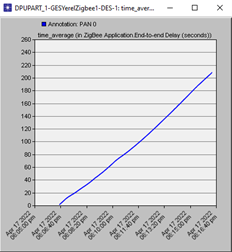
\includegraphics[width=5cm]{Resim/Sekil4-22.png}}


\centering
%ethernet haberleşmesinde LAN gecikme grafiğidir
\pgfplotsset{every axis/.append style={
font=\footnotesize,
thin,
tick style={ultra thin}},
scaled y ticks=false,
yticklabel style = {
/pgf/number format/fixed,
/pgf/number format/precision=5
},
}

    \begin{tikzpicture}
    \begin{axis}[
    xlabel={Simülasyon Süresi (Saniye)},
    ylabel={Uçtan Uca Gecikme (Saniye)},
    grid,
    legend style = {font=\tiny,at={(1,0.8)}, anchor=east}
    ]

\addplot [color=cyan, mark=star, mark repeat =14, mark size = 3]  table [x = Simulation Duration, y = GESYerelZigbee1EndtoendDelayseconds, col sep = comma] {fig4deneme (1).csv};
%\addlegendentry{Ethernet bağlantı gecikme değeri}



\end{axis}
\end{tikzpicture}

\caption{\gls{lan} senaryosunda zigbee sistemindeki yaşanan gecikmenin zamana bağlı değişim grafiği.}
\label{fig:4-23}
\end{figure}

\begin{figure}[htbp]
%\centerline{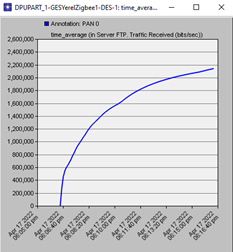
\includegraphics[width=5cm]{Resim/Sekil4-23.png}}

\centering
%ethernet haberleşmesinde LAN gecikme grafiğidir
\pgfplotsset{every axis/.append style={
font=\footnotesize,
thin,
tick style={ultra thin}},
scaled y ticks=false,
yticklabel style = {
/pgf/number format/fixed,
/pgf/number format/precision=5
},
}

    \begin{tikzpicture}
    \begin{axis}[
    xlabel={Simülasyon Süresi (Saniye)},
    ylabel={Yüklenen Veri Boyutu (Byte/s)},
    grid,
    legend style = {font=\tiny,at={(1,0.8)}, anchor=east}
    ]

\addplot [color=blue, mark=circle, mark repeat =14, mark size = 3]  table [x = Simulation Duration, y = GESYerelZigBeeApplicationTrafficReceivedbitssec, col sep = comma] {fig4deneme (1).csv};
%\addlegendentry{Ethernet bağlantı gecikme değeri}



\end{axis}
\end{tikzpicture}


\caption{Yerel ağdaki sunucuya yüklenen veri boyutunun zamana bağlı değişim grafiği.}
\label{fig:4-24}
\end{figure}

\newpage
\paragraph{Rüzgar Enerji Sistemi}
Başlık \ref{zigbeeges112}'daki senaryonun \gls{res} versiyonu \gls{opnet} ortamında simülasyonu tamamlanmıştır. \gls{res}'dekine  ürettiği veri boyutu \gls{ges}'deki algılayı-cılardan fazladır. Bu sebeple Şekil \ref{fig:4-26}'deki veri boyutu Şekil \ref{fig:4-24}'daki yerel sunucuya yüklenen veri boyutundan fazladır. \gls{res}'deki ağ yapısında yaşanan gecikme değerleri Şekil \ref{fig:4-25}'de gösterilmiştir. İlgili gecikme değerleri \gls{iec} 61400 ve \gls{ieee} 1646 standartlarının belirlemiş olduğu gecikme değerlerine göre yüksektir. Bu durumda \gls{res}'deki enerji üretiminin gerçek zamanlı takibi yapılamamaktadır. 

\begin{figure}[htbp]
%\centerline{\includegraphics[width=5cm]{Resim/sekil4-24.png}}
\centering
%ethernet haberleşmesinde LAN gecikme grafiğidir
\pgfplotsset{every axis/.append style={
font=\footnotesize,
thin,
tick style={ultra thin}},
scaled y ticks=false,
yticklabel style = {
/pgf/number format/fixed,
/pgf/number format/precision=5
},
}

    \begin{tikzpicture}
    \begin{axis}[
    xlabel={Simülasyon Süresi (Saniye)},
    ylabel={Uçtan Uca Gecikme (Saniye)},
    grid,
    legend style = {font=\tiny,at={(1,0.8)}, anchor=east}
    ]

\addplot [color=cyan, mark=star, mark repeat =14, mark size = 3]  table [x = Simulation Duration, y = TurbinZigBeeApplicationEndtoendDelayseconds, col sep = comma] {fig4deneme (1).csv};
%\addlegendentry{Ethernet bağlantı gecikme değeri}



\end{axis}
\end{tikzpicture}


\caption{\gls{lan} senaryosunda zigbee sistemindeki yaşanan gecikmenin zamana bağlı değişim grafiği.}\label{fig:4-25}
\end{figure}

\begin{figure}[htbp]
%\centerline{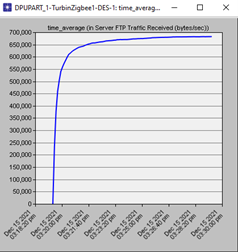
\includegraphics[width=5cm]{Resim/sekil4-25.png}}


\centering
%ethernet haberleşmesinde LAN gecikme grafiğidir
\pgfplotsset{every axis/.append style={
font=\footnotesize,
thin,
tick style={ultra thin}},
scaled y ticks=false,
yticklabel style = {
/pgf/number format/fixed,
/pgf/number format/precision=5
},
}

    \begin{tikzpicture}
    \begin{axis}[
    xlabel={Simülasyon Süresi (Saniye)},
    ylabel={Yüklenen Veri Boyutu (Byte/s)},
    grid,
    legend style = {font=\tiny,at={(1,0.8)}, anchor=east}
    ]

\addplot [color=blue, mark=circle, mark repeat =14, mark size = 3]  table [x = Simulation Duration, y = TurbinZigBeeApplicationTrafficReceived, col sep = comma] {fig4deneme (1).csv};
%\addlegendentry{Ethernet bağlantı gecikme değeri}



\end{axis}
\end{tikzpicture}

\caption{Yerel ağdaki sunucuya yüklenen veri boyutunun zamana bağlı değişim grafiği.}
\label{fig:4-26}
\end{figure}


\newpage
\subsubsection{\gls{lan} tasarımı OPNET Simülasyon Sonuçları}


Zigbee, \gls{wifi} ve Ethernet altyapısında modellenen simülasyonların 2 \gls{myo}'daki sonuçları \ref{yerelEthernet}--\ref{zigbee} başlıklarında paylaşılmıştır. \gls{lan} simülasyon sonuçları incelendiğinde Zigbee altyapısı ile kurulan haberleşme trafiğinde gecikme değerleri ilgili standartların belirlemiş olduğu üst değer olan 1 saniyenin çok üzerindedir. Bu sebeple Geniş Alan Ağı tasarımının olduğu bölümde Zigbee altyapısı dahil edilmemiştir.

\section{OPNET GENİŞ ALAN AĞI TASARIM VE SİMÜLASYON SONUÇLARI}

Önceki bölümde \gls{lan} modeli incelenmiştir. Şekil \ref{fig:4-27}’de Google Earth yazılı-mında Kütahya’nın meslek yüksekokulları ve merkez kampüsü gösterilmiştir. Okullardaki enerji üretim sisteminin merkezi bir noktadan kontrolü gözlemi ve aksiyonu için \gls{iec}, veri haberleşmesinin en fazla 1 saniye gecikmesine izin vermiştir. Tasarım olarak enerji üretiminin izleme merkezi \gls{dpu} Merkez Kampüsü olarak belirlenmiştir. Geniş alan ağı tasarım senaryoları kablosuz ve kablolu olarak iki kısımda incelenmiştir.


\begin{figure}[htbp]
\centerline{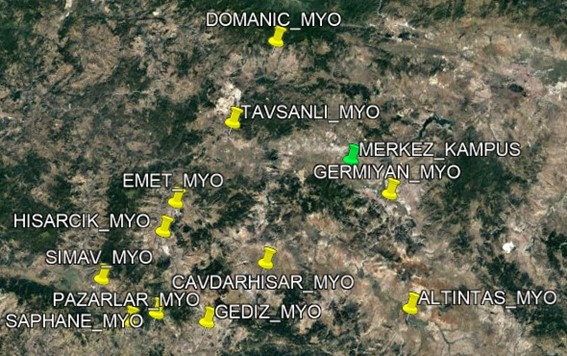
\includegraphics[width=10cm]{Resim/sekil4-26.jpg}}
\caption{\gls{dpu}’nün Meslek Yüksek Okulları ve Merkez Kampüsü}
\label{fig:4-27}
\end{figure}


\subsection{Kablosuz Geniş Ağ Tasarımı}

\ref{mikrohaberlesme} kısmında belirtilen kablosuz haberleşme tekniğinden \gls{wimax} teknolojisi kullanılarak meslek yüksekokulları arasında bir haberleşme linki kurulmuştur. Yüksek hızlarda haberleşme çözümü imkanı sağlayan \gls{wimax} teknolojisi 11-66 GHz arasında bir haberleşme taşıyıcı frekansına sahiptir. Bu frekans aralığındaki elektromanyetik dalganın boyu çok küçüktür. Elektromanyetik dalga için atmosfer soğurumu frekansın karesiyle ters orantılı olduğu için, yüksek frekans bölgesinde düşük kayıplı iletişim için doğrudan görüş hattında iletişim yapılması gereklidir.

İlgi \gls{myo}'ların \gls{dpu} merkez kampüsü ile sağlıklı bir haberleşme sağlaması için öncelikle sistemsel olarak Google Earth yazılımında Kütahya ilinin fiziki yükselti haritası incelenmiştir. Bu incelemelerin sonucunda 2 adet toplama noktası belirlenmiştir. Bu toplama noktaları ile üniversiteye ait kampüslerin birbirlerini doğrudan ve engelsiz bir şekilde görebildiği Google Earth yazılımından doğrulanmıştır.

Toplama noktalarıyla doğrudan haberleşen meslek yüksekokulları Tablo \ref{tab:tablo4-6}'da gösterilmiştir.



\begin{figure}[htbp]
\centerline{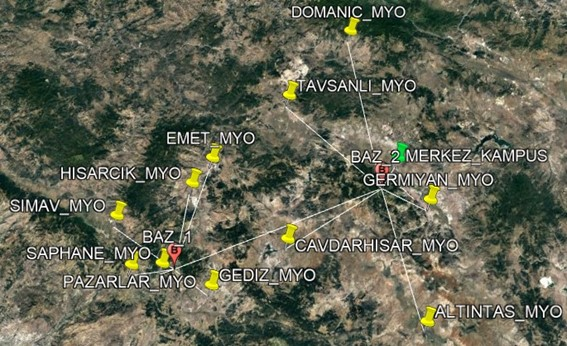
\includegraphics[width=10cm]{Resim/sekil4-27.jpg}}
\caption{Baz istasyonu vaziyet planı}
\label{fig:4-28}
\end{figure}




\begin{table}[htbp]
\centering
\caption{Yerleşkelerde kullanılan enerji sistemi ve bağlı olduğu baz istasyonları.}
\label{tab:tablo4-6}
\begin{tabular}{|l|c|l|c|}
\hline
Yerleşke İsmi        & \multicolumn{1}{l|}{Baz No} & Yerleşke İsmi         & \multicolumn{1}{l|}{Baz No} \\ \hline
Pazarlar \gls{myo} (Güneş) & \multirow{6}{*}{1}          & Tavşanlı \gls{myo} (Rüzgar) & \multirow{6}{*}{2}          \\ \cline{1-1} \cline{3-3}
Hisarcık \gls{myo} (Rüzgar) &  & Domanic \gls{myo} (Rüzgar)    &  \\ \cline{1-1} \cline{3-3}
Şaphane \gls{myo} (Güneş)   &  & Germiyan \gls{myo} (Rüzgar)   &  \\ \cline{1-1} \cline{3-3}
Gediz \gls{myo} (Güneş)     &  & Altıntaş \gls{myo} (Güneş)    &  \\ \cline{1-1} \cline{3-3}
Simav \gls{myo} (Rüzgar)    &  & Çavdarhisar \gls{myo} (Güneş) &  \\ \cline{1-1} \cline{3-3}
Emet \gls{myo} (Rüzgar)     &  & Merkez Kampüs (İzleme)  &  \\ \hline
\end{tabular}
\end{table}


\begin{figure}[htbp]
\centerline{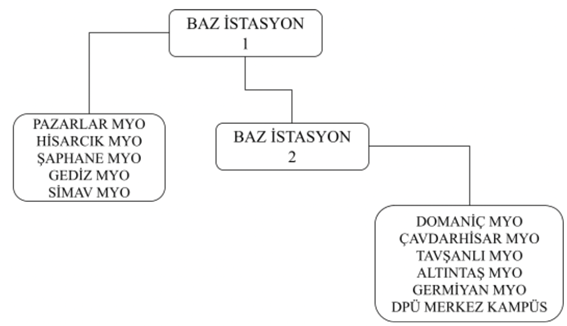
\includegraphics[width=10cm]{Resim/sekil4-28.png}}
\caption{Baz istasyonları bağlantı topolojisi}
\label{fig:4-29}
\end{figure}

\gls{wimax} haberleşmesinde minimum veri kullanımı önemli bir faktördür. Gereksiz veri trafiği en istenmeyen durumdur. Bölüm \ref{motivasyon}'de belirtildiği üzere amaçlanan kriter minimum haberleşme maliyeti ile maksimum performansta bir haberleşme çözümü sunmaktır. Bu nedenle lokal bölgelerde oluşturulan verilerin \gls{dpu} Merkez kampüsüne ileti-lirken diğer lokal bölgelere iletilmesinin önüne geçilmelidir. 

Günümüzde IP haberleşmesinde farklı ağları birbirleriyle haberleştirme tekniği olarak yönlendirme protokolleri kullanılmaktadır. 
Kullanıcı kendi yerel alan ağı dışındaki bir noktaya veri gönderebilmek için yerel ağındaki yönlendiriciye verisini iletir; yönlendi-rici de nihai hedefe doğru verileri iletir. Nihai hedefin yerel alan ağından sorumlu yönlen-diriciye kadar belirli cihazlar arasında atlama yapmaktadır. Uçtan uca yol boyunca her yönlendirici, hedefe ulaşmak için kullanılan bir sonraki atlama cihazını seçer. Sonraki atlama, hedefe ulaşmak için yol boyunca bir sonraki cihazı temsil eder. Böylelikle rotalama tekniği uygulanmış olur. 

IP yönlendirme metodu statik ve dinamik olarak iki kısımda incelenir. Bu tezde veri trafiklerini geniş alan ağlarında yönetmek için statik yönlendirme kullanılmıştır.

Statik yönlendirme, ağ yöneticisi tarafından tasarlanır ve ağa uygulanır. Ağ yöneticisinin sorumluluğunda bütün trafik şekillenmektedir. Statik yönlendirmenin tercih edilme sebepleri aşağıda paylaşılmıştır. \cite{parziale_2006}

•	Yönlendirme algoritmasına göre daha spesifik bir rota içermediğinde trafiği iletmek için tercih edilir.

•	Karmaşık yönlendirme ilkeleri gerektiğinde kullanılır. Örnek olarak, belirli bir ana bilgisayara yönlendirilen trafiğin belirlenmiş bir ağ yolundan geçmesini garanti etmek gibi bir senaryo gerektiğinde statik yönlendirme tekniği kullanılır.

•	Ağ yöneticisi, kurulu sistemde tanımlanan tüm ağların sınıfı veya özelliğine göre birbirleriyle spesifik verilerin haberleşmesini sağlamak için statik yönlendirme kullanmaktadır. 

•	Statik yönlendirme yöntemi, komşu cihazlar arasında rota bilgilerini tanıtmayı gerektirmez. Bu durum sayesinde haberleşmede kullanılan bant genişliğinden tasarruf edilir. Ayrıca, ağ yollarını hesaplamak için daha az işlemci önbelleği ve döngüsü kullanılır.

\gls{wimax} teknolojisinde veri trafiğinde kullanılan bant genişliği çok önemli bir konudur. Bilindiği üzere \gls{wimax} lisanslı bir bant üzerinden haberleşmesini yapmaktadır, yani limitli bir bant genişliği kullanımı söz konusudur. Bu nedenle yerel noktalarda oluşturulan verilerin en az bant genişliği kullanılarak gönderilmesi amaçlanmıştır. Statik yönlendirme tekniği de bu sebepten kullanılmaktadır. Bu teknik sayesinde aynı baz istasyonlarına bağlı farklı meslek yüksekokulları, birbirlerinin haberleşme bant genişliğini işgal etmemektedir. Merkez noktadaki toplama noktasına gönderilen veriler böylelikle korunmuş olur ayrıca başka noktalarda gereksiz veri boyutu kullanımının önüne geçilmiş olur.

\begin{figure}[htbp]
\centerline{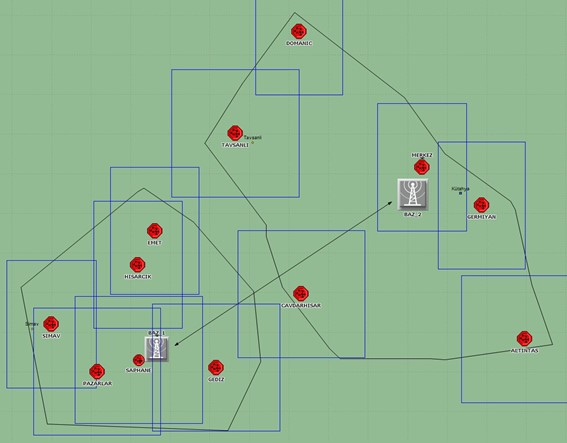
\includegraphics[width=\columnwidth]{Resim/sekil4-29.jpg}}
\caption{OPNET ortamında tasarlanan WAN yerleşim planında iki adet baz istasyonu bulunmaktadır. Baz istasyonlarının kapsama alanları gösterilmiştir. \gls{myo}'larda üretilen tüm veriler baz istasyonları aracılığıyla merkez'e iletilmektedir.}
\label{fig:4-30}
\end{figure}



\subsubsection{Senaryo:1}\label{senaryo1}

\gls{wimax} teknolojisi ile haberleşilen geniş alan ağının ilk senaryosunda \gls{wimax} altyapısı kullanılmıştır. Meslek Yüksekokullarında üretilen algılayıcı verileri \gls{wifi} altya-pısında haberleşmektedir. Yapılan senaryo tasarımı sonrasında tüm \gls{myo}'larda bulunan algılayıcı düğümlerinde gözlemlenen ortalama gecikme (delay) değeri 0.06 saniyedir. Gecikme değeri, aynı haberleşme protokolünde çalışan iki düğüm arasında paket gönde-rim süresi olarak tanımlanmıştır. Şekil \ref{fig:4-31}’de gözlemlenen gecikme değişimi \gls{iec} 61400 ve \gls{iec} 61724 standartlarını karşılamaktadır. 12 adet kampüs içi yerel alan ağının \gls{wifi} üzerinden haberleşme yapılması durumuyla birleştirilmiş \gls{wimax} geniş alan ağı teknolojisinde yaşanan gecikmenin grafiği Şekil \ref{fig:4-31}’de paylaşılmıştır.



\begin{figure}[htbp]
%\centerline{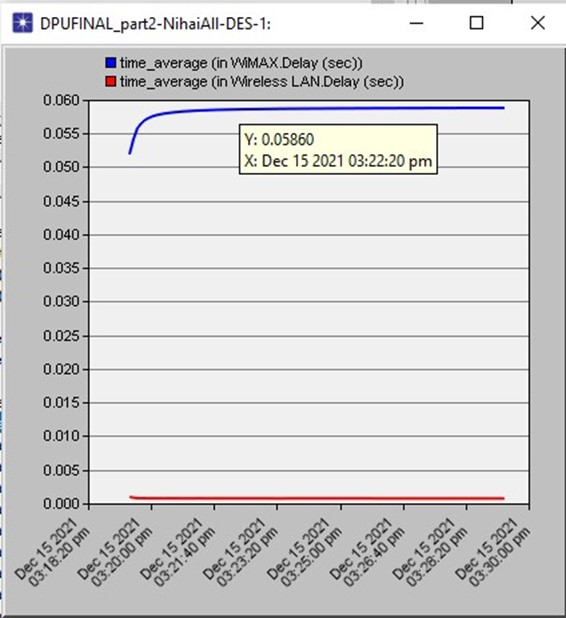
\includegraphics[width=10cm]{Resim/Sekil4-30.jpg}}

\centering
\pgfplotsset{every axis/.append style={
font=\footnotesize,
thin,
tick style={ultra thin}},
}
    \begin{tikzpicture}
\begin{semilogyaxis}[ymax = 0.070000,
xlabel={Simülasyon Süresi (Saniye)},
ylabel={Gecikme Süresi (Saniye)},
xmode=normal, ymode=log, 
grid = major,
log ticks with fixed point,
ytick={0.05,0.0005, 0.01,0.001,0.0001,0.005},
legend style = {font=\tiny,at={(1,0.3)}, anchor=east}
]


\addplot [color=blue, mark=oplus*, mark repeat =14, mark size = 3]  table [x = Simulation Duration, y = Senaryo1WimaxDelay, col sep = comma] {fig4deneme (1).csv};


%--
\addplot [color=red, mark=pentagon*, mark repeat =14, mark size = 3, mark phase = 8]  table [y = Senaryo1WifiDelay, col sep = comma] {fig4deneme (1).csv};

%--

\legend{Wimax Gecikme, WiFi Gecikme }
\end{semilogyaxis}



\end{tikzpicture}


\caption{\gls{wimax} ve \gls{wifi} teknolojisinde gözlemlenen gecikmenin zamana bağlı değişim grafiği.}
\label{fig:4-31}
\end{figure}

\gls{dpu} merkez kampüsünde kurulan ana sunucuya gönderilen toplam veri boyutunun anlık grafiği Şekil \ref{fig:4-32}’de gösterilmiştir. Kurulu olan güneş ve rüzgar enerji sistemlerinde üretilen verilerin toplam boyutu, ana sunucuya gelen veri boyutuyla aynıdır. Şekil \ref{fig:4-32}'e bakarak 11 adet \gls{myo}'da bir veri kaybının olmadığı görülmektedir.

\begin{figure}[htbp]
%\centerline{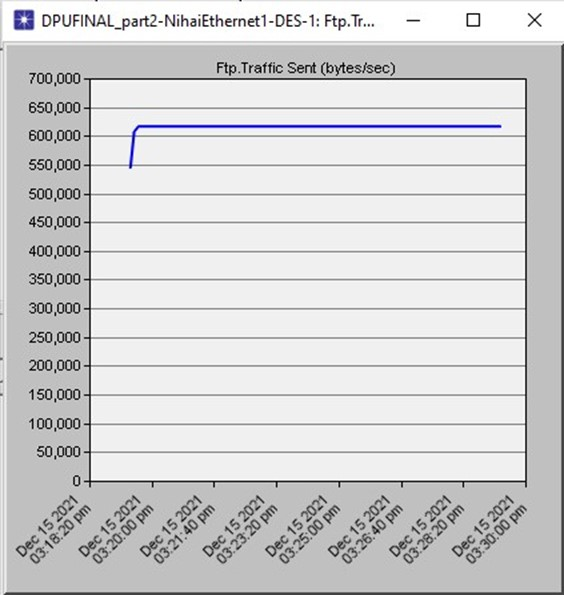
\includegraphics[width=10cm]{Resim/Sekil4-31.jpg}}
\centering
%ethernet haberleşmesinde LAN gecikme grafiğidir
\pgfplotsset{every axis/.append style={
font=\footnotesize,
thin,
tick style={ultra thin}},
scaled y ticks=false,
yticklabel style = {
/pgf/number format/fixed,
/pgf/number format/precision=5
},
}

    \begin{tikzpicture}
    \begin{axis}[ymax = 700000.0000000,
    xlabel={Simülasyon süresi (Saniye)},
    ylabel={Yüklenen Veri Boyutu (Byte/s)},
    grid,
    legend style = {font=\tiny,at={(1,0.8)}, anchor=east}
    ]

\addplot [color=blue, mark=circle, mark repeat =14, mark size = 3]  table [x = Simulation Duration, y = TOTALReceivedAllScenario, col sep = comma] {fig4deneme (1).csv};
%\addlegendentry{Ethernet bağlantı gecikme değeri}



\end{axis}
\end{tikzpicture}


\caption{DPÜ merkez kampüsünde bulunan komuta kontrol merkezine ait ana sucuya yüklenen veri boyutlarının zamana bağlı değişim grafiği.}
\label{fig:4-32}
\end{figure}


Simülasyon sonucunda ana sunucuya gelen algılayıcıların anlık veri boyutları Resim \ref{fig:4-33}’te gösterilmiştir. Örneğin, Tablo \ref{tab:tablo4-5}’teki rüzgar algılayıcılarının ürettikleri veri değeri 6 Byte/s değerindedir, bu durum ile birlikte Tablo \ref{tab:tablo4-4}’teki WROT algılayıcısı 12010 Byte/s değerinde veri üretmektedir. İlgili \gls{wan} senaryosunda 5 adet \gls{ges}, 5 adet \gls{res} bulunmaktadır. Simülasyon sonucunda "Rüzgar Hızı" algılayıcıları toplamda 30 Byte/s'lik, "WROT" algılayıcıları toplamda 72.060 Byte/s'lik hızlarda ana sunucuya veri göndermişlerdir. Farklı algılayıcının üretmiş olduğu veri miktarlarının aynı grafikte birlikte gösterilebilmesi için logaritmik eksen tercih edilmiştir. 
%bunu tablo olarak göster


\begin{comment}

\begin{table}[htbp]
\centering
\caption{Ana sunucada toplanan algılayıcılarıcıların anlık değişimi}
\label{fig:4-33}
\begin{tabular}{cc}
\hline
\begin{tabular}[c]{@{}c@{}}Algılayıcı\\ Tanımı\end{tabular} & \begin{tabular}[c]{@{}c@{}}Merkez Sunucuya\\ İletilen Veri \end{tabular} \\ \hline
Meteoroloji         & 50 B/s         \\
İnverter Akım       & 72.000 B/s         \\
İnverter Gerilim    & 72.000 B/s         \\
Rüzgar Hızı         & 30 B/s    \\
Radyant Işıma       & 1.000 B/s    \\
WCNV                & 75.020 B/s         \\
WGEN                & 70.020 B/s         \\
WMET                & 40.000 B/s    \\
WNAC                & 66.048 B/s    \\
WROT                & 60.050 B/s       \\
WTOW                & 12.036 B/s       \\
WTRF                & 48.036 B/s       \\
WTRM                & 72.096 B/s       \\
WYAW                & 36.024 B/s       \\
WROT                & 60.050 B/s       \\ \hline
TOTAL & 684.460 B/s       \\ \hline
\end{tabular}
\end{table}
\end{comment}




\begin{figure}[htbp]
%\centerline{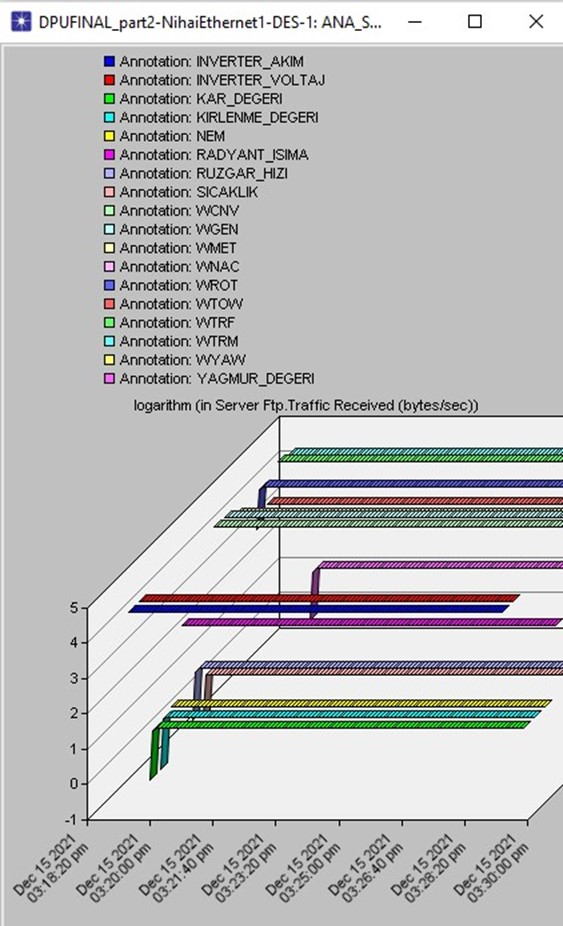
\includegraphics[width=10cm]{Resim/Sekil4-32.jpg}}

\centering
\pgfplotsset{every axis/.append style={
font=\footnotesize,
thin,
tick style={ultra thin}},
scaled y ticks=false,
yticklabel style = {
/pgf/number format/fixed,
/pgf/number format/precision=5
},
}
    \begin{tikzpicture}
\begin{semilogyaxis}[
zmode = log,
zmin = 1,
xlabel={Simülasyon Süresi (Saniye)},
zlabel={Yüklenen Veri Boyutu (Byte/s)},
ytick = \empty,
grid = major,
log ticks with fixed point,
legend style = {font=\tiny,at={(1,0.8)}, anchor=east},
area plot1/.style={%ilk alan için oluşturulan saydanlık vs.
fill opacity=0.33,
draw = orange!80!black,thick,
fill = orange,
mark=none,
},
area plot2/.style={
fill opacity=0.33,
draw = blue!80!black,thick,
fill = blue,
mark=none,
},
area plot3/.style={
fill opacity=0.33,
draw = cyan!80!black,thick,
fill = cyan,
mark=none,
},
area plot4/.style={
fill opacity=0.33,
draw = red!80!black,thick,
fill = red,
mark=none,
},
area plot5/.style={
fill opacity=0.33,
draw = yellow!80!black,thick,
fill = yellow,
mark=none,
},
area plot6/.style={
fill opacity=0.23,
draw = gray!80!black,thick,
fill = gray,
mark=none,
},
area plot7/.style={
fill opacity=0.23,
draw = purple!80!black,thick,
fill = purple,
mark=none,
},
area plot8/.style={
fill opacity=0.23,
draw = green!80!black,thick,
fill = green,
mark=none,
},
legend pos = outer north east,]
%bu kısımda turbinlerin hepsini plot3'e ekliyoruz
\addplot3+ [area plot1]  table [x = Simulation Duration, y = eksen1, z = TrafficReceivedbytessecINVERTERAKIM, col sep = comma] {fig4deneme (1).csv} \closedcycle;
\addlegendentry{İnverter Akım}
%---------

\addplot3+ [area plot1]  table [y = eksen2, z = TrafficReceivedbytessecINVERTERVOLTAJ, col sep = comma] {fig4deneme (1).csv} \closedcycle;
\addlegendentry{İnverter Gerilim}
%---------

\addplot3+ [area plot2]  table [y = eksen3, z = TrafficReceivedbytessecMETEOR, col sep = comma] {fig4deneme (1).csv} \closedcycle;
\addlegendentry{Meteoroloji}
%---------


\addplot3+ [area plot3]  table [y = eksen4, z = TrafficReceivedbytessecRADYANTISIMA, col sep = comma] {fig4deneme (1).csv} \closedcycle;
\addlegendentry{Radyant Işıma}
%---------


\addplot3+ [area plot4]  table [y = eksen5, z = TrafficReceivedbytessecRUZGARHIZI, col sep = comma] {fig4deneme (1).csv} \closedcycle;
\addlegendentry{Rüzgar Hızı}
%---------


\addplot3+ [area plot5]  table [y = eksen6, z = TrafficReceivedbytessecWCNV, col sep = comma] {fig4deneme (1).csv} \closedcycle;
\addlegendentry{WCNV}
%---------

\addplot3+ [area plot6]  table [y = eksen7, z = TrafficReceivedbytessecWGEN, col sep = comma] {fig4deneme (1).csv} \closedcycle;
\addlegendentry{WCNV}
%---------

\addplot3+ [area plot7]  table [y = eksen8, z = TrafficReceivedbytessecWMET, col sep = comma] {fig4deneme (1).csv} \closedcycle;
\addlegendentry{WMET}
%---------


\addplot3+ [area plot2]  table [y = eksen9, z = TrafficReceivedbytessecWNAC, col sep = comma] {fig4deneme (1).csv} \closedcycle;
\addlegendentry{WNAC}
%---------

\addplot3+ [area plot1]  table [y = eksen10, z = TrafficReceivedbytessecWROT, col sep = comma] {fig4deneme (1).csv} \closedcycle;
\addlegendentry{WROT}
%---------


\addplot3+ [area plot3]  table [y = eksen11, z = TrafficReceivedbytessecWTOW, col sep = comma] {fig4deneme (1).csv} \closedcycle;
\addlegendentry{WTOW}
%---------

\addplot3+ [area plot4]  table [y = eksen12, z = TrafficReceivedbytessecWTRF, col sep = comma] {fig4deneme (1).csv} \closedcycle;
\addlegendentry{WTRF}
%---------


\addplot3+ [area plot2]  table [y = eksen13, z = TrafficReceivedbytessecWTRM, col sep = comma] {fig4deneme (1).csv} \closedcycle;
\addlegendentry{WTRM}
%---------

\addplot3+ [area plot2]  table [y = eksen14, z = TrafficReceivedbytessecWYAW, col sep = comma] {fig4deneme (1).csv} \closedcycle;
\addlegendentry{WYAW}
%---------


\end{semilogyaxis}
\end{tikzpicture}


\caption{DPÜ merkez kampüsünde bulunan komuta kontrol merkezine ait ana sunucuya gönderilen algılayıcı verilerinin logaritmik eksendeki zamana bağlı değişim grafiği.}
\label{fig:4-33}
\end{figure}


Tablo \ref{tab:tablo4-6}’ya göre \gls{myo}'larda üretilen algılayıcı verilerinin \gls{dpu} merkez sunu-cusuna gönderilme zamanı Şekil \ref{fig:4-34}’de gösterilmiştir. Şekil \ref{fig:4-34}’de üretilen veriler yaklaşık 0.46 saniyelik gecikme ile ana sunucuda toplandığı gözlemlenmiştir. Geniş alan ağında, \gls{iec} standartlarına göre, verilerin 1 saniyenin altında bir süre ile hedef noktasına iletilmesi gerektiği belirtilmektedir \cite{mackiewicz2006overview}. Buna göre tasarlanan \gls{wifi} ve \gls{wimax} hibrit teknolojili haberleşme ağı ilgili standartları tamamen karşılamaktadır

\begin{figure}[htbp]
%\centerline{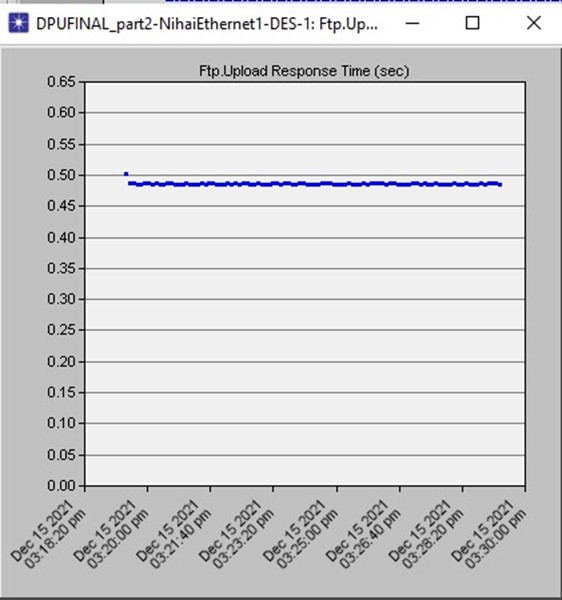
\includegraphics[width=10cm]{Resim/Sekil4-33.jpg}}
\centering
\pgfplotsset{every axis/.append style={
font=\footnotesize,
thin,
tick style={ultra thin}},
scaled y ticks=false,
yticklabel style = {
/pgf/number format/fixed,
/pgf/number format/precision=5
},
}

    \begin{tikzpicture}
    \begin{axis}[
    xlabel={Simülasyon süresi (Saniye)},
    ylabel={Veri Yükleme Süresi (Saniye)},
    grid,
    legend style = {font=\tiny,at={(1,0.8)}, anchor=east}
    ]

\addplot [color=blue, mark=circle, mark repeat =14, mark size = 3]  table [x = Simulation Duration, y = Senaryo1uploadResponseTime, col sep = comma] {fig4deneme (1).csv};
%\addlegendentry{Ethernet bağlantı gecikme değeri}



\end{axis}
\end{tikzpicture}


\caption{11 adet MYO'da çalışan algılayıcı düğümlerinde üretilen veri paketlerinin ana sunucuya yüklenme süresine ait zamana bağlı değişim grafiği.}
\label{fig:4-34}
\end{figure}
\newpage
\subsubsection{Senaryo:2}\label{senaryo2}

11 adet \gls{myo}'da kurulmuş olan UTP altyapılı haberleşme sisteminde gözlemlenen ortalama gecikme değeri Şekil \ref{fig:4-35}’te görüldüğü üzere yaklaşık 0.00015 saniyedir. İlgili MYO'ların \gls{wimax} altyapısındaki ortalama gecikme değeri 0.05 saniyedir. 
Bu değerler, yerel alan ağında \gls{wifi} teknolojisi kullanıldığı duruma göre daha iyidir. 

\begin{figure}[htbp]
%\centerline{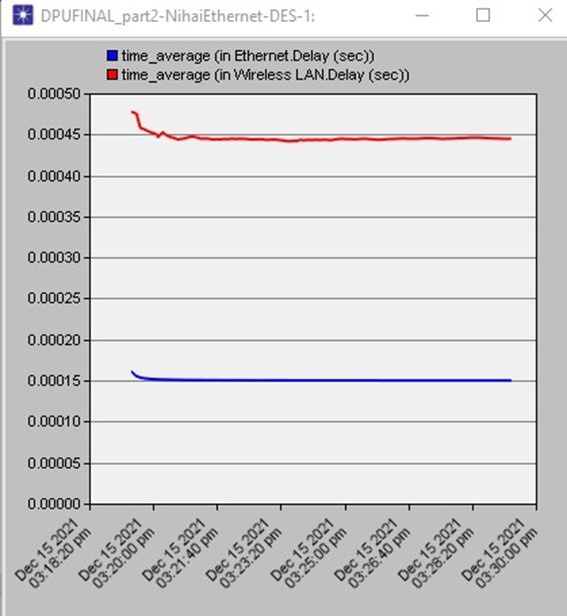
\includegraphics[width=10cm]{Resim/Sekil4-34.jpg}}

\centering
\pgfplotsset{every axis/.append style={
font=\footnotesize,
thin,
tick style={ultra thin}},
}
    \begin{tikzpicture}
\begin{semilogyaxis}[ymax = 0.070000,
xlabel={Simülasyon Süresi (Saniye)},
ylabel={Gecikme Süresi (Saniye)},
xmode=normal, ymode=log, 
grid = major,
log ticks with fixed point,
ytick={0.05,0.0005, 0.01,0.001,0.0001,0.005},
legend style = {font=\tiny,at={(1,0.3)}, anchor=east}
]


\addplot [color=blue, mark=oplus*, mark repeat =14, mark size = 3]  table [x = Simulation Duration, y = Senaryo2WimaxDelay, col sep = comma] {fig4deneme (1).csv};


%--
\addplot [color=red, mark=pentagon*, mark repeat =14, mark size = 3, mark phase = 8]  table [y = Senaryo2UTPEthernet Delay, col sep = comma] {fig4deneme (1).csv};

%--

\legend{Wimax Gecikme, WiFi Gecikme }
\end{semilogyaxis}



\end{tikzpicture}



\caption{\gls{wimax} ve Ethernet teknolojisinde gözlemlenen gecikmenin zamana bağlı değişim grafiği.}
\label{fig:4-35}
\end{figure}

Şekil \ref{fig:4-36}’de \gls{dpu}’nün merkez kampüsünde kurulan ana sunucuya gönderilen toplam verinin değişim grafiğine bakıldığında, bölüm \ref{senaryo1} Şekil \ref{fig:4-32}'deki performans değerleriyle neredeyse aynı olduğu görülmüştür. 


\begin{figure}[htbp]
%\centerline{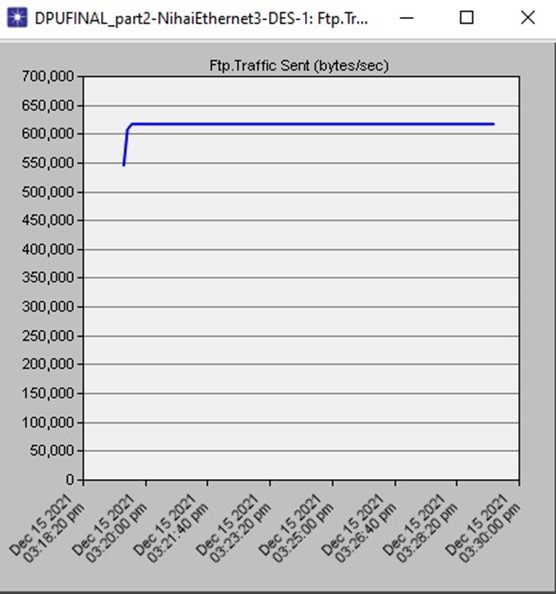
\includegraphics[width=10cm]{Resim/Sekil4-35.jpg}}


\centering
%ethernet haberleşmesinde LAN gecikme grafiğidir
\pgfplotsset{every axis/.append style={
font=\footnotesize,
thin,
tick style={ultra thin}},
scaled y ticks=false,
yticklabel style = {
/pgf/number format/fixed,
/pgf/number format/precision=5
},
}

    \begin{tikzpicture}
    \begin{axis}[ymax = 700000,
    xlabel={Simülasyon süresi (Saniye)},
    ylabel={Yüklenen Veri Boyutu (Byte/s)},
    grid,
    legend style = {font=\tiny,at={(1,0.8)}, anchor=east}
    ]

\addplot [color=red, mark=circle, mark repeat =14, mark size = 3]  table [x = Simulation Duration, y = TOTALReceivedAllScenario, col sep = comma] {fig4deneme (1).csv};
%\addlegendentry{Ethernet bağlantı gecikme değeri}



\end{axis}
\end{tikzpicture}


\caption{DPÜ merkez kampüsünde bulunan komuta kontrol merkezine ait ana sucuya yüklenen veri boyutlarının zamana bağlı değişim grafiği.}
\label{fig:4-36}
\end{figure}


Ana sunucuda toplanan algılayıcıların gerçek zamanlı veri boyutları Şekil \ref{fig:4-37} üzerinde gösterilmiştir. Yerel ağda \gls{wifi} teknolojisi kullanıldığında da aynı değerler elde edilmiştir. Buna göre haberleşme trafiğinde yerel ağ teknolojisinin Ethernet veya \gls{wifi} olma durumu, performans açısından bir fark oluşturmamaktadır.

\begin{figure}[htbp]
%\centerline{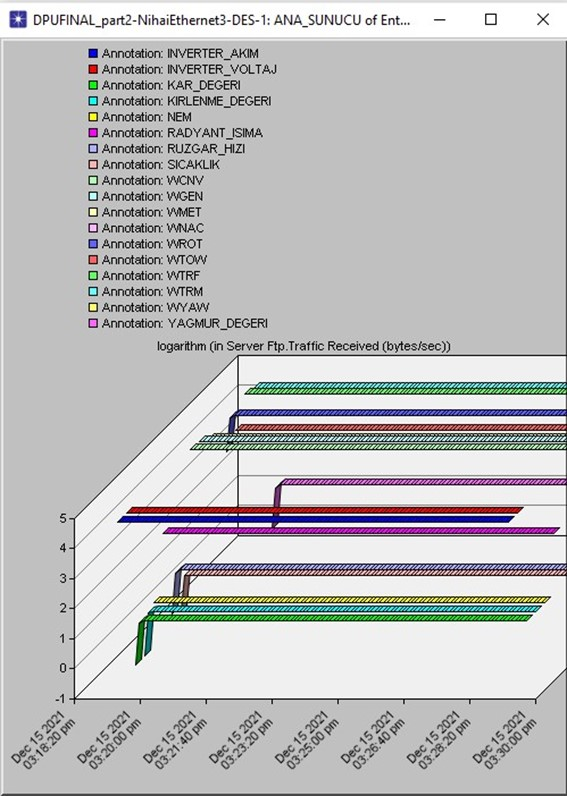
\includegraphics[width=10cm]{Resim/sekil4-36.jpg}}



\centering
\pgfplotsset{every axis/.append style={
font=\footnotesize,
thin,
tick style={ultra thin}},
scaled y ticks=false,
yticklabel style = {
/pgf/number format/fixed,
/pgf/number format/precision=5
},
}
    \begin{tikzpicture}
\begin{semilogyaxis}[
zmode = log,
zmin = 1,
xlabel={Simülasyon Süresi (Saniye)},
zlabel={Yüklenen Veri Boyutu (Byte/s)},
ytick = \empty,
grid = major,
log ticks with fixed point,
legend style = {font=\tiny,at={(1,0.8)}, anchor=east},
area plot1/.style={%ilk alan için oluşturulan saydanlık vs.
fill opacity=0.33,
draw = orange!80!black,thick,
fill = orange,
mark=none,
},
area plot2/.style={
fill opacity=0.33,
draw = blue!80!black,thick,
fill = blue,
mark=none,
},
area plot3/.style={
fill opacity=0.33,
draw = cyan!80!black,thick,
fill = cyan,
mark=none,
},
area plot4/.style={
fill opacity=0.33,
draw = red!80!black,thick,
fill = red,
mark=none,
},
area plot5/.style={
fill opacity=0.33,
draw = yellow!80!black,thick,
fill = yellow,
mark=none,
},
area plot6/.style={
fill opacity=0.23,
draw = gray!80!black,thick,
fill = gray,
mark=none,
},
area plot7/.style={
fill opacity=0.23,
draw = purple!80!black,thick,
fill = purple,
mark=none,
},
area plot8/.style={
fill opacity=0.23,
draw = green!80!black,thick,
fill = green,
mark=none,
},
legend pos = outer north east,]
%bu kısımda turbinlerin hepsini plot3'e ekliyoruz
\addplot3+ [area plot1]  table [x = Simulation Duration, y = eksen1, z = TrafficReceivedbytessecINVERTERAKIM, col sep = comma] {fig4deneme (1).csv} \closedcycle;
\addlegendentry{İnverter Akım}
%---------

\addplot3+ [area plot1]  table [y = eksen2, z = TrafficReceivedbytessecINVERTERVOLTAJ, col sep = comma] {fig4deneme (1).csv} \closedcycle;
\addlegendentry{İnverter Gerilim}
%---------

\addplot3+ [area plot2]  table [y = eksen3, z = TrafficReceivedbytessecMETEOR, col sep = comma] {fig4deneme (1).csv} \closedcycle;
\addlegendentry{Meteoroloji}
%---------


\addplot3+ [area plot1]  table [y = eksen4, z = TrafficReceivedbytessecRADYANTISIMA, col sep = comma] {fig4deneme (1).csv} \closedcycle;
\addlegendentry{Radyant Işıma}
%---------


\addplot3+ [area plot2]  table [y = eksen5, z = TrafficReceivedbytessecRUZGARHIZI, col sep = comma] {fig4deneme (1).csv} \closedcycle;
\addlegendentry{Rüzgar Hızı}
%---------


\addplot3+ [area plot5]  table [y = eksen6, z = TrafficReceivedbytessecWCNV, col sep = comma] {fig4deneme (1).csv} \closedcycle;
\addlegendentry{WCNV}
%---------

\addplot3+ [area plot6]  table [y = eksen7, z = TrafficReceivedbytessecWGEN, col sep = comma] {fig4deneme (1).csv} \closedcycle;
\addlegendentry{WCNV}
%---------

\addplot3+ [area plot7]  table [y = eksen8, z = TrafficReceivedbytessecWMET, col sep = comma] {fig4deneme (1).csv} \closedcycle;
\addlegendentry{WMET}
%---------


\addplot3+ [area plot2]  table [y = eksen9, z = TrafficReceivedbytessecWNAC, col sep = comma] {fig4deneme (1).csv} \closedcycle;
\addlegendentry{WNAC}
%---------

\addplot3+ [area plot1]  table [y = eksen10, z = TrafficReceivedbytessecWROT, col sep = comma] {fig4deneme (1).csv} \closedcycle;
\addlegendentry{WROT}
%---------


\addplot3+ [area plot3]  table [y = eksen11, z = TrafficReceivedbytessecWTOW, col sep = comma] {fig4deneme (1).csv} \closedcycle;
\addlegendentry{WTOW}
%---------

\addplot3+ [area plot4]  table [y = eksen12, z = TrafficReceivedbytessecWTRF, col sep = comma] {fig4deneme (1).csv} \closedcycle;
\addlegendentry{WTRF}
%---------


\addplot3+ [area plot2]  table [y = eksen13, z = TrafficReceivedbytessecWTRM, col sep = comma] {fig4deneme (1).csv} \closedcycle;
\addlegendentry{WTRM}
%---------

\addplot3+ [area plot7]  table [y = eksen14, z = TrafficReceivedbytessecWYAW, col sep = comma] {fig4deneme (1).csv} \closedcycle;
\addlegendentry{WYAW}
%---------


\end{semilogyaxis}
\end{tikzpicture}

\caption{DPÜ merkez kampüsünde bulunan komuta kontrol merkezine ait ana sunucuya gönderilen algılayıcı verilerinin logaritmik eksendeki zamana bağlı değişim grafiği.}
\label{fig:4-37}
\end{figure}

Tablo \ref{tab:tablo4-6}’ya göre meslek yüksek okullarında üretilen algılayıcı verilerinin \gls{dpu} \\komuta merkezi sunucusuna gönderilme zamanı Şekil \ref{fig:4-38}’de gösterilmiştir. Bu grafiğe göre üretilen veriler yaklaşık 0.41 saniyelik gecikme ile ana sunucuda toplandığı gözlemlenir. Geniş ağ teknolojisindeki \gls{iec} standartlarında verilerin 1 saniyenin altında bir süre ile hedef noktasına iletilmesi gerektiği belirtilmektedir \cite{mackiewicz2006overview}. Buna göre tasarlanan Ethernet ve \gls{wimax} hibrit teknolojili haberleşme sistemi ilgili standartları tamamen karşılamaktadır.


\begin{figure}[htbp]
%\centerline{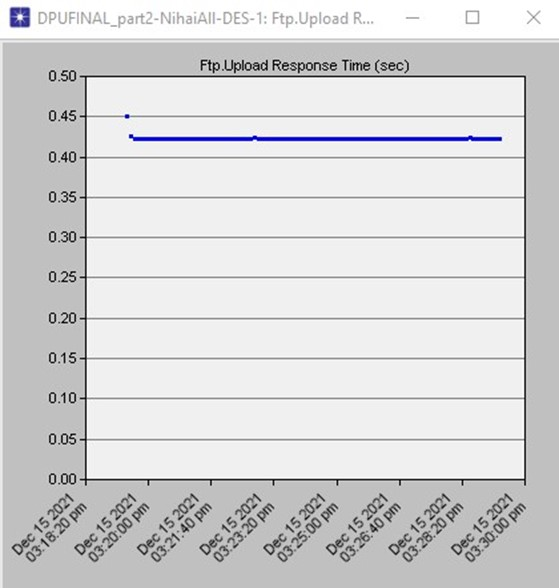
\includegraphics[width=10cm]{Resim/sekil4-37.jpg}}
\centering
%ethernet haberleşmesinde LAN gecikme grafiğidir
\pgfplotsset{every axis/.append style={
font=\footnotesize,
thin,
tick style={ultra thin}},
scaled y ticks=false,
yticklabel style = {
/pgf/number format/fixed,
/pgf/number format/precision=5
},
}

    \begin{tikzpicture}
    \begin{axis}[
    xlabel={Simülasyon süresi (Saniye)},
    ylabel={Veri Yükleme Süresi (Saniye)},
    grid,
    legend style = {font=\tiny,at={(1,0.8)}, anchor=east}
    ]

\addplot [color=blue, mark=circle, mark repeat =14, mark size = 3]  table [x = Simulation Duration, y = Senaryo2uploadResponseTime, col sep = comma] {fig4deneme (1).csv};
%\addlegendentry{Ethernet bağlantı gecikme değeri}



\end{axis}
\end{tikzpicture}


\caption{11 adet MYO'da çalışan algılayıcı düğümlerinde üretilen veri paketlerinin ana sunucuya yüklenme süresine ait zamana bağlı değişim grafiği.}
\label{fig:4-38}
\end{figure}

\newpage
\subsection{Fiber Altyapılı Geniş Ağ Tasarımı}\label{fibeeraciklama}


Yerel internet sağlayıcıları üzerinden tarife anlaşması sağlanarak kurulmaktadır. Fakat telekom hattı sadece \gls{dpu} hizmet vermemekle birlikte hizmet sağladığı noktalardaki başka aboneleriyle birlikte ortak bir haberleşme havuzundan haberleşme hizmeti vermektedir. Bu hizmetin finansal açıdan ilk başta avantajının olması kaçınılmazdır. Fakat üniversiteye bağlı \gls{myo}'ların haberleşme güvenliğinin sağlanması son kullanıcının sorumluluğunda olacaktır. Buna göre ilgili meslek yüksekokullarına kurulacak harici bir güvenlik duvarı ve yönlendirici donanımlarıyla yerel ağlarda toplanan algılayıcı verileri fiziki bir güvenlik duvarından geçerek yönlendiriciler üzerinden \gls{dpu} Merkez kampüsüne ulaşır.


\begin{figure}[htbp]
\centerline{\includegraphics[width=10cm]{Resim/sekil4-39.jpg}}
\caption{Telekom altyapısına ait fiber optik ağın, önerilen dağıtık algılayıcı haberleşme ağına uyarlanması}
\label{fig:4-39}
\end{figure}

Şekil \ref{fig:4-40}’da görüldüğü üzere ana sunucuya iletilen verilerin süresi paylaşılır. Verilerin fiber optik altyapıyla iletilmesi, veri hızı açısından en etkili yöntemdir.

\begin{figure}[htbp]
%\centerline{\includegraphics[width=10cm]{Resim/sekil4-38.jpg}}
\centering
%ethernet haberleşmesinde LAN gecikme grafiğidir
\pgfplotsset{every axis/.append style={
font=\footnotesize,
thin,
tick style={ultra thin}},
scaled y ticks=false,
yticklabel style = {
/pgf/number format/fixed,
/pgf/number format/precision=5
},
}

    \begin{tikzpicture}
    \begin{axis}[
    xlabel={Simülasyon süresi (Saniye)},
    ylabel={Veri Yükleme Süresi (Saniye)},
    grid,
    legend style = {font=\tiny,at={(1,0.8)}, anchor=east}
    ]

\addplot [color=blue, mark=circle, mark repeat =14, mark size = 3]  table [x = Simulation Duration, y = Senaryo2uploadResponseTime, col sep = comma] {fig4deneme (1).csv};
%\addlegendentry{Ethernet bağlantı gecikme değeri}



\end{axis}
\end{tikzpicture}



\caption{Enerji sistemlerindeki algılayıcı verilerin ana sunucuya ortalama ulaşma süresi.Revize}
\label{fig:4-40}
\end{figure}

\section{SİSTEM BİLEŞENLERİNİN MALİYET HESABI}

2022 yılı inşaat ve tesisat birim fiyat kitabına, \gls{dmo} satın alım sayfalarına, Türkiye’de Aselsan AŞ’nin yetkili \gls{wimax} bayisine ve Türk Telekom A.Ş.’nin fiyatlarına bağlı kalınarak, haberleşme sistemlerinde kurulacak malzeme ve işçi-liklerin maliyet tabloları oluşturulmuştur \cite{birimfiyat}.




\subsection{Kablolu Yerel Ağ Haberleşme Altyapısı (Güneş Enerji Sistemi)}


Kablolu haberleşme ağı altyapısında kullanılan malzemelerin maliyeti Tablo \ref{tab:tablo4-7}’de gösterilmiştir.

İlgili tabloya bakıldığında kablolu haberleşmedeki en yüksek maliyet haberleşme sisteminin dış ortam şartlarından korunması için gereken koruyucu ekipmanlarıdır. Çünkü\\ sistemin iletiminde dış ortamdan korunması için endüstriyel ortamlarda kullanılan koruge borusu, bir arıza durumunda müdahale kolaylığı sağlanması için kullanılan menhol malzemeleri, sistemin sürdürülebilirliğini sağlaması için kritik malzemelerdir.


\begin{table}[htbp]
\centering
\caption{\gls{myo} kablolu haberleşme altyapısı maliyet tablosu}

\label{tab:tablo4-7}
\begin{tabular}{ccccr}
\hline
Malzeme tanımı &
  \begin{tabular}[c]{@{}c@{}}Bakanlık Poz\\ Numarası\end{tabular} &
  Maliyet (\Lira) &
  Miktar &
  \multicolumn{1}{c}{Toplam} \\ \hline
FTP Cat6 Kablo                                                       & 35.505.2040          & 10,00\Lira               & 1330 mt & 13.300,00\Lira           \\ \hline
PE Esaslı Menhol                                                     & 10.450.10.57         & 300,00\Lira              & 22 ad   & 6.600,00\Lira            \\ \hline
\begin{tabular}[c]{@{}c@{}}300 mm Anma\\ Çaplı HDPE\\ Koruge Boru\\ Ek Aparatları Dahil\end{tabular} &
  10.450.10.57 &
  70,00\Lira &
  700 mt &
  49.000,00\Lira \\ \hline
\begin{tabular}[c]{@{}c@{}}\gls{utp} Cat6 Patch\\ Panel\end{tabular}       & 35.505.7302          & 1.355,00\Lira            & 1 ad    & 1.355,00\Lira            \\ \hline
\begin{tabular}[c]{@{}c@{}}Dikili Tip Kabinet\\ Tüm Elemanları Dahil\end{tabular} &
  35.550.2000 &
  9.000,00\Lira &
  1 ad &
  9.000,00\Lira \\ \hline
\begin{tabular}[c]{@{}c@{}}Yönetilebilir Ağ\\ Anahtarı\end{tabular} &
  \begin{tabular}[c]{@{}c@{}}7677-K3193\\ (\gls{dmo}\\ ürün kodu)\end{tabular} &
  8.426,66\Lira &
  1 ad &
  8.426,66\Lira \\ \hline
Patch Cord                                                           & 35.545.2105          & 52,00\Lira               & 37 ad   & 1.924,00\Lira            \\ \hline
\begin{tabular}[c]{@{}c@{}}Ethernet Algılayıcı\\ Düğümü\end{tabular} & 35.130.2801          & 1.085,00\Lira            & 27      & 29.295,00\Lira           \\ \hline
\multicolumn{4}{r}{TOPLAM MALİYET} & 118.900,66\Lira
\end{tabular}
\end{table}




\subsection{Kablosuz Yerel Ağ Haberleşme Altyapısı(Güneş Enerji Sistemi)}

\begin{table}[htbp]
\centering
\caption{\gls{myo} Kablosuz haberleşme sistemi maliyet tablosu}

\label{tab:tablo4-8}
\begin{tabular}{ccccr}
\hline
Malzeme tanımı &
  \begin{tabular}[c]{@{}c@{}}Bakanlık Poz\\ Numarası\end{tabular} &
  Maliyet (\Lira) &
  Miktar &
  \multicolumn{1}{c}{Toplam} \\ \hline
Lokal Toplayıcı Anten                                                       & 35.405.2300          & 4.000,00\Lira               & 1 ad & 4.000,00\Lira           \\ \hline
\gls{utp} Cat6 Patch Panel                                                     & 35.505.7301         & 736,00\Lira              & 1 ad   & 736,00\Lira            \\ \hline
\begin{tabular}[c]{@{}c@{}}Dikili Tip Kabinet \\ Tüm Elemanları\\ Dahil\\ \end{tabular} &
  35.550.2000 &
  6.000,00\Lira &
  1 ad &
  6.000,00\Lira \\ \hline
\gls{wifi} Router & \begin{tabular}[c]{@{}c@{}}75464-K3347\\ (\gls{dmo} ürün kodu)\end{tabular}& 8.426,66\Lira            & 1 ad    & 8.426,66\Lira            \\ \hline
Patch Cord                                                           & 35.545.2105          & 52,00\Lira               & 37 ad   & 1.924,00\Lira            \\ \hline
\begin{tabular}[c]{@{}c@{}}\gls{wifi} Algılayıcı\\ Düğümü\end{tabular}  & 35.130.2801          & 1.200,00\Lira               & 27 ad   & 32.400,00\Lira            \\ \hline

\multicolumn{4}{r}{TOPLAM MALİYET} & 53.486,66\Lira
\end{tabular}
\end{table}


Tablo \ref{tab:tablo4-8}’e bakıldığında kablosuz haberleşmedeki en yüksek maliyet kullanılan algılayıcı düğümlerinin \gls{wifi} modüllü olması ve haberleşmenin sorunsuz yapılması için kullanılan toplayıcı antenin maliyetidir. 


\subsection{Kablolu Yerel Ağ Haberleşme Altyapısı (Rüzgar Enerji Sistemi)}


Kablolu haberleşme ağı altyapısında kullanılan malzemelerin maliyeti Tablo \ref{tab:tablo4-10}’de gösterilmiştir.

İlgili tabloya bakıldığında kablolu haberleşmedeki en yüksek maliyet haberleşme sisteminin dış ortam şartlarından korunması için gereken koruyucu ekipmanlarıdır. Çünkü\\ sistemin iletiminde dış ortamdan korunması için endüstriyel ortamlarda kullanılan koruge borusu, bir arıza durumunda müdahale kolaylığı sağlanması için kullanılan menhol malzemeleri, sistemin sürdürülebilirliğini sağlaması için kritik malzemelerdir.


\begin{table}[htbp]
\centering
\caption{\gls{myo} kablolu haberleşme altyapısı maliyet tablosu}

\label{tab:tablo4-10}
\begin{tabular}{ccccr}
\hline
Malzeme tanımı &
  \begin{tabular}[c]{@{}c@{}}Bakanlık Poz\\ Numarası\end{tabular} &
  Maliyet (\Lira) &
  Miktar &
  \multicolumn{1}{c}{Toplam} \\ \hline
FTP Cat6 Kablo                                                       & 35.505.2040          & 10,00\Lira               & 850 mt & 8.200,00\Lira           \\ \hline
PE Esaslı Menhol                                                     & 10.450.10.57         & 300,00\Lira              & 2 ad   & 600,00\Lira            \\ \hline
\begin{tabular}[c]{@{}c@{}}300 mm Anma\\ Çaplı HDPE\\ Koruge Boru\\ Ek Aparatları Dahil\end{tabular} &
  10.450.10.57 &
  70,00\Lira &
  120 mt &
  8.400,00\Lira \\ \hline
\begin{tabular}[c]{@{}c@{}}\gls{utp} Cat6 Patch\\ Panel\end{tabular}       & 35.505.7302          & 736,00\Lira            & 1 ad    & 736,00\Lira            \\ \hline
\begin{tabular}[c]{@{}c@{}}Dikili Tip Kabinet\\ Tüm Elemanları Dahil\end{tabular} &
  35.550.2000 &
  6.000,00\Lira &
  1 ad &
  6.000,00\Lira \\ \hline
\begin{tabular}[c]{@{}c@{}}Yönetilebilir Ağ\\ Anahtarı\end{tabular} &
  \begin{tabular}[c]{@{}c@{}}7677-K3193\\ (\gls{dmo} ürün kodu)\end{tabular} &
  8.426,66\Lira &
  1 ad &
  8.426,66\Lira \\ \hline
Patch Cord                                                           & 35.545.2105          & 52,00\Lira               & 20 ad   & 1.040,00\Lira            \\ \hline
\begin{tabular}[c]{@{}c@{}}Ethernet Algılayıcı\\ Düğümü\end{tabular} & 35.130.2801          & 1.085,00\Lira            & 9      & 9.765,00\Lira           \\ \hline
\multicolumn{4}{r}{TOPLAM MALİYET} & 43.167,66\Lira
\end{tabular}
\end{table}

\subsection{Kablosuz Yerel Ağ Haberleşme Altyapısı (Rüzgar Enerji Sistemi)}

Kablolu haberleşme ağı altyapısında kullanılan malzemelerin işçilikli maliyeti Tablo \ref{tab:tablo4-9}’de gösterilmiştir.


\begin{table}[htbp]
\centering
\caption{Rüzgar enerji sisteminin kurulduğu \gls{myo}'ya ait kablosuz haberleşme altyapısı maliyet tablosu}

\label{tab:tablo4-9}
\begin{tabular}{ccccr}
\hline
Malzeme tanımı &
  \begin{tabular}[c]{@{}c@{}}Bakanlık Poz\\ Numarası\end{tabular} &
  Maliyet (\Lira) &
  Miktar &
  \multicolumn{1}{c}{Toplam} \\ \hline
Lokal Toplayıcı Anten                                                       & 35.405.2300          & 4.000,00\Lira               & 1 ad & 4.000,00\Lira           \\ \hline
\gls{utp} Cat6 Patch Panel                                                     & 35.505.7301         & 736,00\Lira              & 1 ad   & 736,00\Lira            \\ \hline
\begin{tabular}[c]{@{}c@{}}Dikili Tip Kabinet \\ Tüm Elemanları\\ Dahil\\ \end{tabular} &
  35.550.2000 &
  6.000,00\Lira &
  1 ad &
  6.000,00\Lira \\ \hline
\gls{wifi} Router & \begin{tabular}[c]{@{}c@{}}75464-K3347\\ (\gls{dmo} ürün kodu)\end{tabular}& 8.426,66\Lira            & 1 ad    & 8.426,66\Lira            \\ \hline
Patch Cord                                                           & 35.545.2105          & 52,00\Lira               & 18 ad   & 936,00\Lira            \\ \hline
\begin{tabular}[c]{@{}c@{}}\gls{wifi} Algılayıcı\\ Düğümü\end{tabular}  & 35.130.2801          & 1.200,00\Lira               & 9 ad   & 10.800,00\Lira            \\ \hline

\multicolumn{4}{r}{TOPLAM MALİYET} & 30.898,66\Lira
\end{tabular}
\end{table}




\subsection{Kablosuz Geniş Ağ Haberleşme Altyapısı}



Geniş ağ haberleşmesinde \gls{wimax} standartlarını uyarlayabilmek için 2 adet baz istasyonu kurulmuştur. Bu baz istasyonlarına, meslek yüksekokullarındaki abone erişim noktaları bağlanmıştır. Bu erişim noktaları sayesinde \gls{wimax} bandında bir haberleşme sistemi kurulmuştur. Kurulacak baz istasyonların olduğu bölgede Orman Genel Müdürlüğü\\  ile anlaşması yapılan \gls{gsm} kulelerinin yapıldığı varsayılmıştır. Hali hazırda kurulu olan \gls{gsm} kulelerinin enerji ve kule altyapısına \gls{wimax} antenleri ve baz istasyonları kolayca entegre edildiği düşünülmüştür.
Bu varsayıma göre Tablo \ref{tab:tablo4-11}'de gösterilen kule kurulum maliyetinden muaf sayılmıştır.







WAN haberleşme projesinde kurulacak olan \gls{wimax} bileşenlerinin maliyetleri Tablo \ref{tab:tablo4-12}'de gösterilmiştir.


\begin{table}[htbp]
\centering
\caption{Geniş alan ağı \gls{wimax} haberleşme sistemi maliyeti}

\label{tab:tablo4-12}
\begin{tabular}{ccccr}
\hline
Malzeme tanımı &
  \begin{tabular}[c]{@{}c@{}}Maliyet\\ Referansı\end{tabular} &
  Maliyet (\Lira) &
  Miktar &
  \multicolumn{1}{c}{Toplam} \\ \hline
\begin{tabular}[c]{@{}c@{}}\gls{wimax} anten\\ Meslek yüksekokullarında\\ kullanılan  \end{tabular} & Global Forte          & 40.000,00\Lira               & 12 ad & 480.000,00\Lira           \\ \hline
\begin{tabular}[c]{@{}c@{}}\gls{wimax} Baz \\ İstasyonu\\ \end{tabular} &
  Global Forte &
  150.000,00\Lira &
  2 ad &
  300.000,00\Lira \\ \hline

\multicolumn{4}{r}{TOPLAM MALİYET} & 780.000,00\Lira
\end{tabular}
\end{table}
Tablo \ref{tab:tablo4-11}'de oluşturulan maliyet, Orman Genel Müdürlüğü \gls{gsm} baz istasyonu kule boyune göre asgari keşif özetleri yazısında bahsedilen kalem fiyatlarına göre oluşturulmuştur \cite{ogm_2009}.


\begin{table}[htbp]
\centering
\caption{30 metrelik \gls{wimax} baz istasyonunu kulesinin yapım maliyeti}

\label{tab:tablo4-11}
\begin{tabular}{ccccr}
\hline
Malzeme tanımı &
  \begin{tabular}[c]{@{}c@{}}Bakanlık Poz\\ Numarası\end{tabular} &
  Maliyet (\Lira) &
  Miktar &
  \multicolumn{1}{c}{Toplam} \\ \hline
\begin{tabular}[c]{@{}c@{}}El ile geniş \\kazı yapılması \end{tabular}                      & 14.013/1          & 22,30\Lira               & 49,27 m & 1.098,72\Lira           \\ \hline
Dolgu sıkıştırılması                                                     & 14.018         & 4,61\Lira              & 22,487 m   & 103,67\Lira            \\ \hline
\begin{tabular}[c]{@{}c@{}}Gronülomatik kum ve \\kırmataş ile yapılan\\demirli (BS.16) betonu \end{tabular} &
  16.036/2 &
  119,85\Lira &
  8,530 m\textsuperscript{3} &
  1.022,32\Lira \\ \hline
\begin{tabular}[c]{@{}c@{}}Düz yüzeyli \\beton ve betonarme \end{tabular}                    & 21.011  & 16,08\Lira               & 27,096 m\textsuperscript{3}   & 435,7\Lira            \\ \hline
\begin{tabular}[c]{@{}c@{}}200 dozlu \\demirsiz beton \end{tabular}                    & 16.002  & 101,34\Lira               & 1,136 m\textsuperscript{3}   & 115,12\Lira            \\ \hline
\begin{tabular}[c]{@{}c@{}} Q8 -- Q12mm lik \\beton çelik çubuğun\\bükülüp yerine konması \end{tabular}                    & 23.014  & 1.478,75\Lira               & 0,379 m\textsuperscript{3}   & 560,45\Lira            \\ \hline
\begin{tabular}[c]{@{}c@{}} Q14 -- Q28mm lik \\beton çelik çubuğun\\bükülüp yerine konması \end{tabular}                    & 23.015  & 1.384,06\Lira               & 5,383 m\textsuperscript{3}   & 7.450,39\Lira            \\ \hline
\begin{tabular}[c]{@{}c@{}} Çeşitli demir\\işlerin yapılması\\yerine konulması \end{tabular}                    & 23.176  & 4,74\Lira               & 6.800 ad   & 32.368,00\Lira            \\ \hline
\begin{tabular}[c]{@{}c@{}} Paratoner \end{tabular}                    & 980-100  & 25,00\Lira               & 1 ad   & 25,00\Lira            \\ \hline

\begin{tabular}[c]{@{}c@{}} 25mm elektrolitik\\ bakır tel \end{tabular}                    & 981-102  & 8,90\Lira               & 40 m   & 356,00\Lira            \\ \hline

\begin{tabular}[c]{@{}c@{}} Bina ihata\\ iletkeni tesisatı \end{tabular}                    & 982-101  & 19,70\Lira               & 10 ad   & 197,00\Lira            \\ \hline
\begin{tabular}[c]{@{}c@{}} Toprak elektrotu \end{tabular}                    & 983-101  & 196,40\Lira               & 1 ad   & 196,40\Lira            \\ \hline
\begin{tabular}[c]{@{}c@{}} Kafes tel\\ çift ihata \end{tabular}                    & \cite{ogm_2009}  & 42,66\Lira               & 40 ad   & 1.706,40\Lira            \\ \hline

\begin{tabular}[c]{@{}c@{}} Konteynır malzeme\\ ve montaj \end{tabular}                    & \cite{ogm_2009}  & 5.600,00\Lira               & 1 ad   & 5.600,00\Lira            \\ \hline

\begin{tabular}[c]{@{}c@{}} Kollektör borusu\\ galvanizli \end{tabular}                    & 109-103  & 44,00\Lira               & 18 ad   & 792,00\Lira            \\ \hline



\multicolumn{4}{r}{TOPLAM MALİYET} & 52.027,17\Lira
\end{tabular}
\end{table}







\subsection{Telekom Altyapılı \gls{wan} Haberleşme Altyapısı}
Geniş ağ haberleşmesinde Telekom altyapısının kiralanması yoluyla veri akışı sağlanması gerektiği \ref{fibeeraciklama} numaralı başlık altında açıklanmıştır. Üniversite ile Telekom firması arasında yapılacak kurumsal internet sözleşmesiyle aylık abonelik anlaşması ile birlikte üniversitenin meslek yüksekokullarında ve ana kampüsünde yönlendirici, güvenlik duvarı, omurga anahtar kullanılması gerekmektedir. İlgili bileşenlerin maliyeti Tablo \ref{tab:tablo4-13}’te gösterilmiştir.

\begin{table}[htbp]
\centering
\caption{Geniş alan ağı fiber optik haberleşme altyapı maliyeti}

\label{tab:tablo4-13}
\begin{tabular}{ccccr}
\hline
Malzeme tanımı &
  \begin{tabular}[c]{@{}c@{}}Bakanlık Poz\\ Numarası\end{tabular} &
  Maliyet (\Lira) &
  Miktar &
  \multicolumn{1}{c}{Toplam} \\ \hline
\begin{tabular}[c]{@{}c@{}}Router  \end{tabular} & \begin{tabular}[c]{@{}c@{}}85978-K1415\\(\gls{dmo} ürün kodu)  \end{tabular}          & 16.853,31\Lira               & 12 ad & 202.239,72\Lira           \\ \hline
\begin{tabular}[c]{@{}c@{}}Güvenlik Duvarı  \end{tabular} &\begin{tabular}[c]{@{}c@{}}94555-K2929\\(\gls{dmo} ürün kodu)  \end{tabular}
   &
  48.687,35\Lira &
  2 ad &
  584.248,20\Lira \\ \hline
  \begin{tabular}[c]{@{}c@{}}Ana omurga\\ anahtar\end{tabular} &\begin{tabular}[c]{@{}c@{}}8654-K3115\\(\gls{dmo} ürün kodu)  \end{tabular}
   &
  58.050,31\Lira &
  1 ad &
  58.050,31\Lira \\ \hline
\begin{tabular}[c]{@{}c@{}}Telekom\\ fiber internet\\ paketi\end{tabular} &\begin{tabular}[c]{@{}c@{}}100 Mbps\\  \end{tabular}
   &
  10.000,00\Lira &
  24 ay &
  240.000,00\Lira \\ \hline

\multicolumn{4}{r}{TOPLAM MALİYET} & 1.084.538,23\Lira
\end{tabular}
\end{table}



























Yenilenebilir enerji kaynaklarının gerçek zamanlı durum ve üretimin gözlemlenmesi ile ilgili Kütahya Dumlupınar Üniversitesi (DPÜ) merkez kampüs ve bağlı uzak 11 kampüsün bağlı olduğu bir haberleşme ağında veri iletim süreleri açısında performansı ortaya koyan ve IEC standartlarını karşılayıp karşılamadığını test eden modelleme ve simülasyon çalışmaları yapılmıştır. Yerel alan ağları incelendiğinde, Zigbee standardının kullanılması durumunda veri paket kaybının oluşmadığı görülmesine rağmen yerel ağda kurulacak bir gözlem merkezine iletilen verinin gecikme süresi ve yerel sunucuya yüklenen ölçüm verilerinin süresi 1 saniyenin üzerindedir. Bu durum, \gls{iec}'nin belirlemiş olduğu standartları karşılamamaktadır. Bu nedenle yerel noktalarda Zigbee haberleşme tekniğinin kullanılması uygun değildir. Yerel noktalarda Ethernet ve \gls{wifi} standartlarında kullanılacak donanımların ayrı ayrı simülasyonları yapılıp sonuç grafikleri incelendiğinde ilgili standartların tamamen karşılandığı görülmüştür. 

\gls{lan} haberleşme maliyet tabloları incelendiğinde, \gls{wifi} tekniğinin kullanıldığı Güneş Enerji Sisteminin kablolu haberleşme tekniğine göre \%55 oranında daha az maliyetli olduğu hesaplanmıştır. Bu oran Rüzgar Enerji Sistemi için \%28’dir. Rüzgar Enerji Sistemi, daha merkezi bir topolojiye sahip olduğundan, haberleşme maliyeti güneş enerji sistemine göre daha düşüktür.

\gls{wan} tasarımında durum değerlendirildiğine fiber optik haberleşme sisteminin gecikme \gls{wimax} teknolojisine göre çok düşük olduğu gözlemlenmiştir. 

Telekom altyapısıyla bir haberleşme trafiği sağlandığında, haberleşme sisteminin dışarıya karşı korumasız kalmaması için uygulanan güvenlik prosedürlerinin maliyeti fazladır. \gls{wimax} altyapısı kullanıldığında tamamen izole bir ağ kurulmuş olacaktır, ordu standartlarında bir güvenlik şifrelemesi ile paket trafiğinin güvenliği sağlanmış olur.

Geniş ağ tasarımında fizibilite analizinin son kriteri ise sürdürülebilir yapıda olmasıdır. \gls{wimax} altyapısı kullanılırken, baz istasyonlarının olduğu kuleler şehirden uzak dağlık alanlara yerleştirilmiştir. Kulelerde bir problem yaşanması durumunda, arıza müdahale ekibinin ulaşması maliyetli bir süreçtir. Fakat Telekom altyapısında bir problem yaşanması durumunda tüm sorumluluk Telekom firmasına ait olacaktır. 

İlgili kriterler dikkate alınarak hesaplanan maliyetler  Tablo \ref{tab:tablo5-1}’de gösterilmiştir.

\begin{table}[htbp]
\centering
\caption{Karar tablosu}
\label{tab:tablo5-1}
\begin{tabular}{|c|c|c|}
\hline
Çözüm cinsi                               & \gls{lan} & \gls{wan}        \\ \hline
En düşük maliyetli çözüm                     & \gls{wifi}           & \gls{wimax}                 \\ \hline
Sürdürülebilir çözüm                      & \gls{wifi}           & Kiralık fiber ağ \\ \hline
Güvenli iletişim ve en düşük maliyetli çözüm & \gls{wifi}           & \gls{wimax}                 \\ \hline
\end{tabular}

\end{table}


Kütahya Dumlupınar Üniversitesi'ne bağlı 11 kampüste Yenilenebilir Enerji Santralleri kurulması durumunda haberleşme sisteminin maliyetleri ve \gls{opnet} yazılımı sayesinde haberleşme sistemlerinin performansları incelenmiştir. Yenilenebilir Enerji Santralleri'nin gerçek zamanlı performans takibi ilk önceliktir. Tablo \ref{tab:tablo5-1}'deki sunulan çözümler Yenilenebilir Enerji Sistemleri için IEC 61850, IEC 61400 ve IEEE 1646 standartlarında belirtilmiş olan kriterler tamamen karşılanmaktadır.


Üniversitenin bünyesinde üreteceği enerji sistemlerinin sağlık durumlarının ve verimlerinin takibini personel maliyetlerini minimize ederek çözmesi üniversitenin mali bütçesi açısından en mantıklı çözüm olacaktır. Bu temel nedene göre Tablo \ref{tab:tablo5-1}'deki sürdürülebilir çözümün tercih edilmesi mantıklı olacaktır.



%gecenlerde tekrar geziyordum bakım ne goreyim\gls{dpu}

\bibliography{ref.bib}
\printglossary[type=\acronymtype]






\end{document}
